\documentclass[11pt,%                        % primary font size
              a4paper,%                     % A4
              twoside,openright,%          % double sided
              titlepage,%                   % new page after the title
              headinclude,footinclude,%    % header at foot of the page
              %BCOR5mm,%                     % 5 mm bookbinding
              numbers=noenddot,%            % no point after section number
              cleardoublepage=empty,%       % empty pages without header at 
]{scrreprt} % KOMA class

\usepackage{textcomp}                       % fix warning with missing font 
\usepackage{scrhack} % fix warnings when using KOMA with listings package
\usepackage{mparhack,fixltx2e,relsize} % typographical niceties

\usepackage[eulerchapternumbers,   % chapter numbers font: Euler
            beramono,%             % fixed-width font: Bera Mono
            eulermath,%            % math font: AMS Euler
            pdfspacing,%           % better line filling
            listings,%             % listings
            dottedtoc,%            % align TOC page numbers to right
            floatperchapter,       % float objects numbered by chapter
            pdfspacing,
            linedheaders,
            ]{classicthesis}       % classicthesis style
\usepackage{arsclassica} % improve classicthesis
\usepackage[left=4cm,right=3cm,top=3cm,bottom=3cm]{geometry}
\usepackage[english]{babel}
\usepackage[utf8x]{inputenc}
\usepackage[T1]{fontenc}
\usepackage{amsmath,amsfonts,amssymb,amsthm}
\usepackage{lettrine}
\usepackage{graphicx}
\usepackage{float} % to create the new float named Algorithm
\usepackage{clrscode}
\usepackage[colorinlistoftodos,prependcaption,textsize=tiny]{todonotes}
\usepackage{tikz}
\usetikzlibrary{fit}
\usepackage{tikzscale}
\usepackage{appendix}
\usepackage{longtable}
\usepackage{tkz-graph}
\usepackage{tabularx}
\usepackage{caption}
\usepackage{subcaption}
\usepackage{rotating}
\usepackage{hyphenat}
\usepackage{afterpage}

\usepackage[section]{placeins} % to avoid floats going too far
\newfloat{Algorithm}{tbp}{lop}
\definecolor{halfgray}{gray}{0.55}
\PassOptionsToPackage{hyphens}{url}
% To make interline 1.5
%\usepackage{setspace}
%\setstretch{1.5}
%\usepackage{frontespizio}
% \titleformat{\chapter}[block]%
%         {\normalfont\Large\sffamily}%
%         {{\color{halfgray}\chapterNumber\thechapter%
%         \hspace{10pt}\vline}  }{10pt}%
%         {\spacedallcaps}[\chapterdecoration]
% % To enable decoration
% \newcommand\chapterdecoration{\begin{tikzpicture}[remember picture,overlay,shorten >= -10pt]

\coordinate (aux1) at ([yshift=-15pt]current page.north east);
\coordinate (aux2) at ([yshift=-410pt]current page.north east);
\coordinate (aux3) at ([xshift=-4.5cm]current page.north east);
\coordinate (aux4) at ([yshift=-150pt]current page.north east);

\begin{scope}[halfgray!40,line width=12pt,rounded corners=12pt]
\draw
  (aux1) -- coordinate (a)
  ++(225:5) --
  ++(-45:5.1) coordinate (b);
\draw[shorten <= -10pt]
  (aux3) --
  (a) --
  (aux1);
\draw[opacity=0.6,halfgray,shorten <= -10pt]
  (b) --
  ++(225:2.2) --
  ++(-45:2.2);
\end{scope}
\draw[halfgray,line width=8pt,rounded corners=8pt,shorten <= -10pt]
  (aux4) --
  ++(225:0.8) --
  ++(-45:0.8);
\begin{scope}[halfgray!70,line width=6pt,rounded corners=8pt]
\draw[shorten <= -10pt]
  (aux2) --
  ++(225:3) coordinate[pos=0.45] (c) --
  ++(-45:3.1);
\draw
  (aux2) --
  (c) --
  ++(135:2.5) --
  ++(45:2.5) --
  ++(-45:2.5) coordinate[pos=0.3] (d);   
\draw 
  (d) -- +(45:1);
\end{scope}
\end{tikzpicture}}
% \setlength{\headheight}{1.1\baselineskip}

\pgfdeclarelayer{background}
\pgfsetlayers{background,main}

%\usepackage[running]{lineno}
%\linenumbers
\let\marginpar\oldmarginpar

\hypersetup{colorlinks = false, hidelinks }


\newcommand\blankpage{%
    \null
    \thispagestyle{empty}%
    \addtocounter{page}{-1}%
    \newpage}
%\documentclass[a4paper,twoside]{book}
\usepackage[english]{babel}
\usepackage[utf8x]{inputenc}
\usepackage{amsmath,amsfonts,amssymb,amsthm}
%\usepackage[sc]{mathpazo} % Use the Palatino font
%\usepackage{microtype} % Slightly tweak font spacing for aesthetics
\usepackage{graphicx}
\usepackage{hyperref}
\usepackage{float} % to create the new float named Algorithm
%\usepackage{clrscode}
\usepackage[colorinlistoftodos,prependcaption,textsize=tiny]{todonotes}
\usepackage{tikz}
\usetikzlibrary{fit}
\usepackage{tikzscale}
\usepackage{appendix}
\usepackage{longtable}
\usepackage{tkz-graph}
\usepackage{tabularx}
\usepackage{caption}
\usepackage{subcaption}
\usepackage{microtype}

\newfloat{Algorithm}{tbp}{lop}
\linespread{1.12} % Line spacing - Palatino needs more space between lines

\definecolor{halfgray}{gray}{0.55}



% To compile the figures separately, use 
%\usetikzlibrary{external}
%\tikzexternalize[prefix=figures/]

\pdfsuppresswarningpagegroup=1
\title{Community detection in the modular structure of brain functional connectivity networks}
\author{Carlo Nicolini}

%\date{\today}

\newtheorem{obs}{Observation}
\newtheorem{props}{Proposition}
\newenvironment{bottompar}{\par\vspace*{\fill}}{\clearpage}

\begin{document}
%% \begin{frontespizio}
% \Universita{Verona}
% \Logo{images/univr.png}
% \Facolta{Pennutologia}
% \Corso{Nanoscienze e tecnologie avanzate}
% \Dipartimento{ciccio}
% \Annoaccademico{2013-2016}
% \Titolo{Graph analysis of brain functional connectivity}
% \Sottotitolo{Breaking the resolution limit with Surprise}
% \Candidato[123456]{Carlo Nicolini}
% \Relatore{Angelo Bifone}
% \Relatore{Pasquina Marzola}
% %\Correlatore{Ugo Frogio}
% %\Correlatore{Ubaldo Kutuzu}
% \end{frontespizio}

\begin{titlepage}
	% if you want the titlepage to be centered, uncomment and
	% fine-tune the line below (KOMA classes environment)
	% \begin{addmargin}[-1cm]{-3cm}
    \begin{figure}[!h]
    \flushleft
	
\includegraphics[width=0.25\columnwidth]{images/univr.png}
	\end{figure}

    \begin{center}
    	\large
        \textsc{\large{Università degli studi di Verona}}
        \hfill
        \vfill
		\textsc{\large{Dipartimento di diagnostica e sanità pubblica}}
		\vfill
        \textsc{Dottorato di ricerca in nanoscienze e tecnologie avanzate}\\
        Curriculum in Nanomedicina Morfologica Clinica\\
		XIX Ciclo
		\vfill
        \begingroup
       		\huge\textbf{
            The modular structure of brain functional connectivity networks:\\a graph theoretical approach
            }
            \bigskip
        \endgroup
        \vfill
        S.S.D. FIS/07
		\flushleft 
		\normalsize{\textbf{Coordinatore}:}\\
		\medskip {Franco Tagliaro}
		\flushleft
		\normalsize{\textbf{Tutor}:}\\
		\medskip{Angelo Bifone}\\
		\medskip{Pasquina Marzola}\\
        \flushright
        \normalsize{\textbf{Dottorando:}}\\
        \medskip {Carlo Nicolini}\\	
		
        \vfill
        \centering{\textbf{Keywords}:\\Brain networks, modularity, community detection, functional connectivity, Surprise.}

        \vfill
		\centering {A.A. 2014-2017}

    \end{center}  
  %\end{addmargin}       
\end{titlepage}

%%%%%%%%%%%%%%%%% SECOND PAGE %%%%%%%%%%%%%%%%%
% \vspace*{\fill}
% \begin{footnotesize}
% \begin{centering}
% \noindent \copyright 2017 Carlo Nicolini \\
% \url{nicolini.carlo@gmail.com}\\
% Quest’opera è stata rilasciata con licenza Creative Commons Attribuzione – non commerciale non opere derivate 3.0 Italia. Per leggere una copia della licenza visita il sito web:

% \url{http://creativecommons.org/licenses/by-nc-nd/3.0/it/}.

% \begin{flushleft}
% \textbf{Attribuzione:} Devi riconoscere una menzione di paternità adeguata, fornire un link alla licenza ed indicare se sono state effettuate delle modifiche. Puoi fare ciò in qualsiasi maniera ragionevole possibile, ma non con modalità da suggerire che il licenziante avalli e o il tuo utilizzo del materiale.\\
% \textbf{Non commerciale:}  Non puoi usare il materiale per scopi commerciali.\\\textbf{Non opere derivate} Se remixi, trasformi il materiale o ti basi su di esso, non puoi distribuire il materiale così modificato.
% \end{flushleft}

% Graph analysis of brain functional connectivity – Carlo Nicolini \\
% Tesi di Dottorato\\
% Verona, 10 Febbraio 2017 \\
% ISBN XXX \\
% \end{centering}
% \end{footnotesize}
%%%%%%%%%%%%%%%%% SECOND PAGE %%%%%%%%%%%%%%%%%
\thispagestyle{empty}
\hyphenation{Bar-the-le-my}
\hyphenation{For-tu-na-to}
\hyphenation{Lan-ci-chi-net-ti}
\hyphenation{Ra-dic-chi}
% \hyphenation{ana-ly-sis}
% \hyphenation{ori-gi-nal}
% \hyphenation{si-mi-lar}
% \hyphenation{mo-dels}
\maketitle
\pagenumbering{roman}

\tableofcontents
\listoftodos

\chapter*{Acknowledgment}
I am using this opportunity to express my gratitude to everyone who supported me throughout the course of this PhD.
I am thankful for their aspiring guidance, invaluably constructive criticism and patience of my supervisor Prof. Angelo Bifone.



\chapter*{Symbols and Notations}
%\begin{table}[htb!]
%\noindent\begin{tabular}{@{}*{4}{p{\textwidth}@{}}}
\begin{longtable}{@{}*{3}{p{\textwidth}@{}}}
$V$ \quad {\color{gray!50}\hrulefill} \quad  A set of $n$ vertices (or nodes) \\
$E$ \quad {\color{gray!50}\hrulefill} \quad  A set of $m$ edges (or links) \\
$G=(V,E)$ \quad {\color{gray!50}\hrulefill} \quad  A graph with its vertices and edges \\
$n$ \quad {\color{gray!50}\hrulefill} \quad  The number of nodes in $G$ \\
$m$ \quad {\color{gray!50}\hrulefill} \quad  The number of edges in $G$ \\
%$p$ \quad {\color{gray!50}\hrulefill} \quad  number of vertex pairs $p=\binom{n}{2}$\\
$\mathbf{A}$ \quad {\color{gray!50}\hrulefill} \quad  Adjacency matrix of a graph \\
$\mathbf{W}$ \quad {\color{gray!50}\hrulefill} \quad  Weighted adjacency matrix of a graph \\
$C_n$ \quad {\color{gray!50}\hrulefill} \quad  Cycle graph with $n$ vertices \\
$K_n$ \quad {\color{gray!50}\hrulefill} \quad  Clique or complete graph with $n$ vertices \\
$\mathbf{H}(\sigma)$ \quad {\color{gray!50}\hrulefill} \quad  Hamiltonian (energy) of a partition \\
$\mathbf{I}$ \quad {\color{gray!50}\hrulefill} \quad  Identity matrix \\
$\mathbf{L}$ \quad {\color{gray!50}\hrulefill} \quad  Laplacian matrix of a graph \\
$\Pr(\cdot)$ \quad {\color{gray!50}\hrulefill} \quad  Probability distribution \\
$\mathcal{Q}^N$ \quad {\color{gray!50}\hrulefill} \quad  Modularity function \\
$S$ \quad {\color{gray!50}\hrulefill} \quad  Surprise function \\
$\mathcal{S}_a$ \quad {\color{gray!50}\hrulefill} \quad  Asymptotical Surprise function \\
$\delta(i,j)$ \quad {\color{gray!50}\hrulefill} \quad  Kronecker delta \\
$\left<\cdot \right>$ \quad {\color{gray!50}\hrulefill} \quad  Expected (average value) \\
$P_{ij}$ \quad {\color{gray!50}\hrulefill} \quad  Null model \\
$\| \cdot \|_F$ \quad {\color{gray!50}\hrulefill} \quad  Frobenius norm \\
$\sigma$ \quad {\color{gray!50}\hrulefill} \quad  Partition (membership)\\
$\sigma_i$ \quad {\color{gray!50}\hrulefill} \quad  Community index of vertex $i$ \\
$\mathbf{1}$ \quad {\color{gray!50}\hrulefill} \quad  Vector of all $1$ \\
$k,k^{\textrm{out}},k^{\textrm{in}}$ \quad {\color{gray!50}\hrulefill} \quad  undirected, outgoing and incoming degree \\
$k^{\textrm{int}},k^{\textrm{ext}}$ \quad {\color{gray!50}\hrulefill} \quad  internal and external degree \\
$s,s^{\textrm{out}},s^{\textrm{in}}$ \quad {\color{gray!50}\hrulefill} \quad  undirected, outgoing and incoming strength \\
$s^{\textrm{int}},s^{\textrm{ext}}$ \quad {\color{gray!50}\hrulefill} \quad  internal and external strength \\
$\Gamma(u)$ \quad {\color{gray!50}\hrulefill} \quad  Neighboring vertices of vertex $u$
\end{longtable}
%\end{tabular}
%\end{table}

\section*{Acronyms}
In this paragraph we introduce the acronyms used in the rest of this thesis.

\begin{longtable}{@{}*{4}{p{\textwidth}@{}}}
BOLD \quad {\color{gray!50}\hrulefill} \quad  Blood Oxygen Level Dependent \\
CNM \quad {\color{gray!50}\hrulefill} \quad  Clauset-Newman-Moore \\
CPM \quad {\color{gray!50}\hrulefill} \quad  Constant Potts Model \\
ER \quad {\color{gray!50}\hrulefill} \quad  Erdos-Renyi \\
FC \quad {\color{gray!50}\hrulefill} \quad  Functional Connectivity \\
LFR \quad {\color{gray!50}\hrulefill} \quad  Lancichinetti-Fortunato-Radicchi model \\
LM \quad {\color{gray!50}\hrulefill} \quad  Louvain method \\
MOD \quad {\color{gray!50}\hrulefill} \quad  Modularity \\
fMRI \quad {\color{gray!50}\hrulefill} \quad  Functional Magnetic Resonance Imaging \\
RB \quad {\color{gray!50}\hrulefill} \quad  Reichardt-Bornholdt \\
TMS \quad {\color{gray!50}\hrulefill} \quad  Transcranial magnetic stimulation \\
EEG \quad {\color{gray!50}\hrulefill} \quad  Electroencefalography \\
WCC \quad {\color{gray!50}\hrulefill} \quad  Weakly connected component \\
PACO \quad {\color{gray!50}\hrulefill} \quad  PArtitioning Cost Optimization \\
FAGSO \quad {\color{gray!50}\hrulefill} \quad  Fast Agglomerative Surprise Optimization \\
SA \quad {\color{gray!50}\hrulefill} \quad  Simulated Annealing 
\end{longtable}

\section*{Information theory}
%\begin{table}
%\noindent\begin{tabular}{@{}*{4}{p{\textwidth}@{}}}
\begin{longtable}{@{}*{4}{p{\textwidth}@{}}}
$H(X)$ \quad {\color{gray!50}\hrulefill} \quad  Shannon Entropy of $X$ \\
$H(X,Y)$ \quad {\color{gray!50}\hrulefill} \quad  Joint Entropy \\
$H(X|Y)$ \quad {\color{gray!50}\hrulefill} \quad  Conditional Entropy \\
$I(x)$ \quad {\color{gray!50}\hrulefill} \quad  Information of event $x$ \\
$I(X,Y)$ \quad {\color{gray!50}\hrulefill} \quad  Mutual information \\
$NMI(X,Y)$ \quad {\color{gray!50}\hrulefill} \quad  Normalized Mutual Information \\
$rNMI(X,Y)$ \quad {\color{gray!50}\hrulefill} \quad  Relative Normalized Mutual Information \\
$\Pr(x)$ \quad {\color{gray!50}\hrulefill} \quad  Probability to observe $x$ \\
$\Pr(x,y)$ \quad {\color{gray!50}\hrulefill} \quad  Joint probability \\
$\Pr(x|y)$ \quad {\color{gray!50}\hrulefill} \quad  Conditional probability
%\end{tabular}
%\end{table}
\end{longtable}

\chapter*{Synopsis}\label{chap:synopsis}
\lettrine{S}{t}arting from 19th century’s neuron doctrine, we know that the brain is an incredibly complex system of intercommunicating elements, the neurons, intertwined with other cells that support neuronal activity. 
The dynamical processes running on the biological substrate of neurons are the basis of information processing that gives rise to cognitive and psychological processes, from the perception of the external environment to the representation of mental states and emotions.
Neuroscience tackles the investigation of the brain, the most complex organ in nature, at different scales. The molecular and cellular neuroscience is interested at the finest level of working of the nervous system cells. At this scale, molecular biology and genetics are the tools of investigation, as the interest is mainly addressed to very small populations of neurons. 
Larger number of neurons, though needs a more comprehensive view to identify diseases and pathological states. This view must shift from the microscopic level to the so-called system neuroscience, that deals with highly connected networks of neuron, dubbed neuronal circuits.

The interest of systems neuroscience is how these large-scale circuits form and take shape during the life of the organism, how they produce basic processes like reflexes, motor coordination, circadian rhythms and, ultimately, how they give rise to overt behavioral and different internal neural states like motivation, emotions, and cognition.
The extension of systems neuroscience from the study of small groups of neurons to the whole brain will require radically different computational and experimental tools.

Very small scale neuronal circuits that can be studied by mathematically accurate models are formed by several hundreds neurons. The typical size of the smallest identified functional units, the cortical columns, is around hundred thousand neurons and, at that level, many approximation are needed to approximately reproduce the electrical and chemical activity of neurons, at the point that a comprehensive differential equations model of cortical columns is still lacking. 

Finally, a large scale understanding of the incredibly complicated network of all the neurons in the human brain, the human connectome, remains an idealistic (and hotly debated) target to be reached in the future. This scientific, technological and cultural challenge is named after the term ``connectomics'', and aims to map all the connections in the brain at different scales of resolution. Whether will help answer some of the deepest questions about the human brain, it is not entirely known and still a topic of hot debate.

This effort takes advantage of well-consolidated technologies for looking at the brain at work. These non-invasive methods of analysis of brain functions include neuroimaging techniques like magnetic resonance imaging (MRI), electroencephalography (EEG) and transcranial magnetic stimulation (TMS). Among these modalities, MRI, has emerged as a dominant non-invasive imaging method because it enables the investigation of both brain structure and function with a good compromise in terms of spatial and temporal resolution.

At the morphological level, MRI provides a comprehensive view of the brain, as it can identify the white matter fiber pathways connecting gray matter regions otherwise impossible to obtain in-vivo. The pattern of white matter fibers is often called structural connectivity as it relates to the morphological features of the brain connections. With a metaphor, structural connectivity is the analog to the electrical wirings of the different parts of a microprocessor.

Since its inception, the evolution of technologies in MRI, lead to fMRI, a way to spatially map temporal changes of oxygenated blood concentration in the whole brain. This tool helped scientists to unveil another pattern of connectivity that exists in the brain; less substantial than structural connectivity, but nonetheless important as it reveals the dynamics of the brain at work. The term functional connectivity names the pattern of temporal fluctuations of neuronal activities from different brain regions that give rise to changes in blood oxygenation dynamics.

Considered over the large scale, functional connectivity is descriptive of the temporal metabolic demands of large groups of cortical and subcortical structures, a quantity strictly related to the electrical activity of neurons, and yields precious information about the brain not only on its surface but also in other deeper regions, otherwise difficult to reach.
Throughout the years, fMRI helped neuroscientists and neurologists to enrich the knowledge of the fundamental aspects of the normal brain functional organization. Activations maps have been estimated for almost every kind of cognitive task and together with the lesion studies accumulated over two centuries, they greatly increased the awareness of many aspects of brain organization.

Although conceptually simpler than activations studies, even more interesting is the discovery that when a person is cognitively at rest, the brain engages in a characteristic pattern of dynamic neural activity and most brain regions show spontaneous oscillations in the BOLD signal. These fluctuations show correlations that define a network of spatially remote but similar patterns of signal. These networks consisting in highly correlated subsets of brain regions are altered in neuropsychiatric diseases such as autism and schizophrenia.

One of the most important ideas upon which this work is based is that, is possible to quantify the extent of alteration of the aforementioned resting state networks in the diseased brain using the theoretical framework of complex networks science. Complex network science offers the best tools to assess the topology and organization of brain connectivity networks, as well as powerful means to establish, in a completely data-driven manner, diagnoses of common neurological diseases and additionally design lines of intervention and prevention. Under this light, the brain is seen as a network whose elements are the brain regions at different scales, interconnected by a number of links, describing the strength of interregional coordination.

Strong experimental evidence shows that the nervous system in animals and humans, from the neuronal level up to macroscopic levels, displays an organization that favors the exchange of information over a communication backbone supported by well-connected areas, the hubs of the network, responsible in turn for sending information to local processors. The functional brain network in humans and other animals, consist of connected subnetworks (or modules) associated with cognitive functions, of vital importance for the daily life and the interaction in the environment.

While only the biology of the nervous system can detail the etiology of neurological diseases, their observable symptoms often result in a partial or total reorganization of the functional and structural architecture of the brain. In this respect, the definition and validation of actual data-driven biomarkers based on the effects of the disease on the brain is, ultimately, a highly desirable target to reach within the next years.

Among the network level changes observed in the diseased brain, the alteration of the hierarchical and modular structure of both structural and functional brain connectivity is the most recognizable. Using the tools of graph theory, a branch of combinatorial mathematics describing the properties of structures defined by interconnected entities, the evaluation of functional alterations in the modular structure of FC networks is cast to the problem of community detection in graphs, i.e. the problem of identifying independent groups of brain regions that exhibit strong interconnection between each other but that are weakly connected to other modules. Once the graph is partitioned into smaller groups (or communities) of functionally connected modules, it’s, therefore, simpler to quantify the effect of the disease on the partitioning, as well as the areas involved in such reorganization and the role of the single nodes inside their modules.

A methodological problem that passed largely unnoticed in the neuroscience literature of the last years comes from a fundamental issue in community detection and is known as the resolution limit. This barrier has its roots in the theoretical foundations of community detection and practically implies that the detection of brain modules smaller than a scale determined by the size of the total network in exam is very difficult, or in the worst case, even impossible. This limit hampers the ability to detect small scale structures of functionally correlated brain areas and, last, to notice alterations in connectivity between groups of patients and healthy control. Such limit is therefore of impediment to an implementation of a clinical-level biomarker of brain disease.

This work analyzes the implications of the resolution limit in real-world functional connectivity networks and presents a solution to this issue.
The algorithms and analysis methods developed and detailed in the following chapters give an alternative view on the modular structure of the brain and show that, the human brain functional networks present a rich variety of large and small subnetworks, and that the emergence of a heterogeneous distribution of size of functional modules, takes part in shaping the adaptive behavior of the dynamic brain.

The first problem that is addressed in this thesis is therefore how to get rid at least partially of the resolution limit. 
After the demonstration and validation on synthetic benchmarks of a method that mitigates the resolution limit, the second part is devoted to the application to real-world networks. Particular emphasis will be given to a study of the functional differences between resting state fMRI functional networks between two populations of healthy controls and schizophrenic patients. 

In the first chapter, after a brief introduction to the basic terminology of graph theory, I will describe the current approaches to community detection and show how the resolution limit is an intrinsic problem of many of them. After expanding the concepts of the resolution limit, I will then present Surprise optimization as a potential solution, accompanying with examples and validations on some benchmark networks. An extension of Surprise to weighted networks, the most common format of networks encountered in studying functional connectivity, will be the last part of chapter.

The second chapter gives an overview of the modular structure of the brain at different levels, from anatomical to functional. I will continue to show how the resolution limit affected many studies of brain modularity in the literature and to what extent the results obtained by standard methods are different than those obtained with Surprise optimization, illustrating point by point the advantages but also the pitfalls.

The third chapter collects the results obtained on real-world brain networks using the methods introduced in this thesis. The most important result is the application of Asymptotical Surprise optimization to the delineation of functional differences in schizophrenic patients. As the main finding, I will show a functional segregation of some of the major networks of the brain and a general reorganization of the modular structure of the functional connectivity.

All the mathematical details regarding the implementation and the theoretical properties of the methods are collected in an appendix, together with a series of possible tuning that may be in order in future studies.

\section*{Selected publications}
Most of the work presented in this thesis has been submitted or published in journals and conferences. My original contribution~\cite{nicolini2016} is the first demonstration that Surprise is a suitable quality function for community detection on brain functional connectivity.
The paper also shows numerically that Surprise is resolution-limit free in the range of network size of interest in brain functional connectivity.
The second published contribution~\cite{nicolini2017} is the application of an extension of community detection based on Surprise, to weighted networks, together with an analysis that indicates that the resolution limit played an important role as it was hiding from view many important functional structures.

\pagenumbering{arabic}

\chapter*{Abstract}
Complex networks theory offers a framework for the analysis of brain functional connectivity as measured by magnetic resonance imaging.
Within this approach the brain is represented as a graph comprising nodes connected by links, with nodes corresponding to brain regions and the links to measures of inter-regional interaction.
A number of graph theoretical methods have been proposed to analyze the modular structure of these networks.
The most widely used metric is Newman's Modularity, which identifies modules within which links are more abundant than expected on the basis of a random network. However, Modularity is limited in its ability to detect relatively small communities, a problem known as ``resolution limit''.
As a consequence, unambiguously identifiable modules, like complete sub-graphs, may be unduly merged into larger communities when they are too small compared to the size of the network.
This limit, first demonstrated for Newman's Modularity, is quite general and affects, to a different extent, all methods that seek to identify the community structure of a network through the optimization of a global quality function.
Hence, the resolution limit may represent a critical shortcoming for the study of brain networks, and is likely to have affected many of the studies reported in the literature.
This work pioneers the use of Surprise and Asymptotical Surprise, two quality functions rooted in probability theory that aim at overcoming the resolution limit for both binary and weighted networks.
Hereby, heuristics for their optimization are developed and tested, showing that the resulting optimal partitioning can highlight anatomically and functionally plausible modules from brain connectivity datasets, on binary and weighted networks.
This novel approach is applied to the partitionining of two different human brain networks that have been extensively characterized in the literature, to address the resolution-limit issue in the study of the brain modular structure.
Surprise maximization in human resting state networks revealed the presence of a rich structure of modules with heterogeneous size distribution undetectable by current methods.
Moreover, Surprise led to different, more accurate classification of the network's connector hubs, the elements that integrate the brain modules into a cohesive structure.
In synthetic networks, Asymptotical Surprise showed high sensitivity and specificity in the detection of ground-truth structures, particularly in the presence of noise and variability such as those observed in experimental functional MRI data.
Finally, the methodological advances hereby introduced are shown to be an helpful tool to better discern differences between the modular organization of functional connectivity of healthy subjects and schizophrenic patients.
Importantly, these differences may point to new clinical hypotheses on the aetiology of schizophrenia, and they would have gone unnoticed with resolution-limited methods.
This may call for a revisitation of some of the current models of the modular organization of the healthy and diseased brain.
In short, Surprise and Asymptotical represent a promising alternative to current methods, and demonstrate the presence of functional modules of very different sizes in resting state networks.

\chapter{Introduction}\label{chap:introduction}
%This introductory chapter presents the framework of complex network science as applied to brain functional connectivity and analyzes the implications of the resolution limit in real-world networks.
% The brain is an extremely complex organ, whose dynamics is driven by the internal activity of its constituents, the neurons, responding adaptively to an ever-changing outside environment.
% The neurons interact over the organic substrate that they themselves define, and shape an extremely intricate pattern of electrical and metabolic activities, giving rise to the outstanding set of abilities and possibilities typical of most evolved organisms.
% Nonetheless, the notion that brain function can be reduced to the single operations of its constituents is as flawed as its complementary idea that cognition can be understood without making reference to its biological substrate.
% Instead, what science is increasingly recognizing is that, for the description of most systems in nature, it is necessary to remain within a certain level of complexity and to contemplate the multiple interactions of simple subsystems taken as a whole.
% It is known, indeed that many systems, despite radically different at their microscopic level, share many remarkable organizational properties, when analyzed in their entirety.
% A window over the formidable and irreducible complexity of the brain can thus be opened by specific theoretical tools able to account for the brain multi-scale organization, its hierarchical structure, and its modular composition.
% The study of brain connectivity has already made possible many advances in neuroscience, from the identification and structural characterization of the cytoarchitecture to the macro-scale connectivity at the level of nerve fibers.
% Specifically, the analysis of the architecture of the nervous system is based on the idea that the brain can be thought as a complex system at different spatial and time scales.
% In this respect, the tools of network theory are the method of election in the analysis of complex systems.

\section{The rise of network neuroscience}
Starting from 19th century’s neuron doctrine, the brain is described as an incredibly complex system of intercommunicating elements, the neurons, intertwined with other cells that support neuronal activity.

The dynamical processes running on the biological substrate of neurons are the basis of information processing that gives rise to cognitive and psychological processes, from the perception of the external environment to the representation of mental states and emotions.
Neuroscience tackles the investigation of the brain, the most complex organ in nature, at different scales.
Molecular and cellular neuroscience focus on the finest level of workings of the nervous system cells.
At this scale, molecular biology and genetics are used to address the study of very small populations of neurons.

At larger scales, hundreds or thousands of neurons are involved and a more comprehensive approach is needed.
The view must shift from the microscopic level to the so-called systems neuroscience, which deals with widespread networks of neurons, dubbed neuronal circuits.

System neuroscience studies how these large-scale circuits form and evolve during  development, how they produce basic processes like reflexes, motor coordination, circadian rhythms and, ultimately, how they give rise to behavioural and different internal states like motivation, emotions, and cognition.
Hence, an extension of system neuroscience from the study of small groups of neurons to the whole brain requires radically different tools, both computational and experimental.
Very small scale neuronal circuits can be studied by mathematically accurate models.
The typical size of the smallest identified functional unit, the cortical column, is around hundred thousand neurons and, already at that level, many hypotheses are required to approximately reproduce the electrical and chemical activity of neurons, at the point that a comprehensive differential equations model of cortical columns is still lacking.

Yet, a large-scale understanding of the incredibly complicated network of all the neurons in the human brain, the \emph{human connectome}, remains a challenging target to be reached in the future~\cite{amunts2016}.
This scientific, technological and cultural challenge is named after the term \emph{connectomics}, a word coined at the beginning of this decade by Giulio Tononi and Olaf Sporns~\cite{sporns2005}.
Its most ambitious aim is to map all the connections in the brain at different scales of resolution, deep down to the synaptic level.
Whether this will help answer some of the deepest questions about the human brain, it is not entirely known and still a topic of hot debate in the scientific community.

The science of brain connectivity takes advantage of well-consolidated technologies for looking at the brain at work.
These non-invasive methods of analysis of brain functions include neuroimaging techniques like magnetic resonance imaging (MRI), electroencephalography (EEG) and transcranial magnetic stimulation (TMS).
Among these modalities, MRI has emerged as a dominant non-invasive imaging method because it enables the investigation of both brain structure and function with a good compromise in terms of spatial and temporal resolution.

At the morphological level, MRI provides a comprehensive view of the brain, as it can identify the white matter fiber pathways connecting gray matter regions otherwise impossible to obtain in-vivo.
The pattern of white matter fibers is often named after the term \emph{structural connectivity} as it relates to the morphological features of the brain connections.
Structural networks correspond to a pattern of anatomical connections, summarizing bundles of axons connecting different brain regions.
Borrowing ideas from the electronics, structural connectivity may be interpreted as the electrical wiring of the different parts of a processor.
Although useful, the wiring diagram of the brain is only a starting point for making hypotheses about the brain at work; indeed it cannot reveal how neurons behave in real-time, nor does it account for the yet unknown regulatory mechanisms that neurons exert on each other.
Unfortunately, these dynamics are and remain partially unpredictable, despite many notable and useful attempts~\cite{deco2008}, as also the synaptic weights are changing dynamically due to synaptic plasticity.

The discovery of the BOLD effect in the 90's by Ogawa~\cite{ogawa1990}, led to functional MRI, a method to spatially map activity in the whole brain.
Considered over the large scale, the BOLD response is descriptive of the temporal metabolic demands of large groups of cortical and subcortical structures, a quantity strictly related to the electrical activity of neurons~\cite{logothetis2001}.
Indeed an active exchange of information between neural populations is thought to be at the hearth of the BOLD fMRI signal~\cite{logothetis2001}.
The local increase of metabolic demand for oxygenated blood to fuel the neuronal activity increments the vascular flow and favors the consumption of oxygen from neurons.
This metabolic cascade results in the change of the magnetic properties of hemoglobin that transitions from oxygenated to deoxygenated state, yielding local magnetic susceptibility variations measured by MRI.
Possible confounds of the fMRI signal, such as the influence of the cardiac and respiratory rhythms on the BOLD oscillations have been ruled out by a number of studies~\cite{cordes2000,cordes2001,logothetis2001,shmuel2002}.

The tools offered by fMRI helped scientists to unveil another pattern of connectivity that exists in the brain.
\emph{Functional connectivity} examines functional associations between temporal fluctuations of neuronal activities from different brain regions~\cite{biswal1995}.
Activation maps have been estimated for almost every kind of cognitive task and collected in publicly available datasets, like the BrainMap database~\cite{fox2002}, the Neurovault repository~\cite{gorgolewski2015} and the UCLA multimodal connectivity database~\cite{brown2012}.
%Specifically fMRI functional connectivity focuses on the underlying physiological dynamics giving rise to changes in blood oxygenation.
%Since its inception, the evolution of technologies in MRI, lead to functional MRI (fMRI), a way to spatially map temporal changes of oxygenated blood concentration in the whole brain, the so-called BOLD signal.
%Throughout the years, fMRI helped neuroscientists and neurologists to enrich the knowledge of the fundamental aspects of the normal brain functional organization, but as every technique also has its limitations~\cite{logothetis2008}.
% and yields precious information about the brain not only on its surface but also in other deeper regions, otherwise difficult to reach.
In contrast to structural connectivity, functional connectivity results from estimates of statistical dependencies between neuronal or regional time courses.
Functional networks may vary over time, unlike structural networks which are stable over long time scales.
For instance, electrical patterns of cortical activity may rearrange over time-scales of milliseconds, in contrast to structural ones, involved in processes like nervous system development, learning and aging.
Furthermore, the temporal evolution of functional networks is variable as it exhibits spontaneous changes during rest and characteristic modulations for different task conditions~\cite{honey2007,hutchison2013}.
%Importantly, functional connectivity does not express any causal effects between brain regions, as it's only informative of their statistical dependence.
%Together with the lesion studies accumulated over two centuries, they greatly increased the awareness of many aspects of brain organization.

When cognitively at rest, the brain engages in a characteristic pattern of dynamic neural activity and most brain regions show spontaneous oscillations in the BOLD signal~\cite{biswal1995,raichle2001,gusnard2001}. In the resting state, a subject is quietly awake and alert but does not engage in or attend to any specific cognitive or behavioral task.
Interestingly, this background activity dubbed \emph{resting-state connectivity}, is not extinguished but only attenuated during tasks~\cite{fransson2006}, making evident its importance in response to changes in the external demands.
During a typical resting state fMRI (rs-fMRI) session, volunteers are left in the MRI scanner, instructed to relax and not to think anything in particular.
On the other end, animals like mice or rats, are lightly sedated and the BOLD signal is measured for longer time intervals, yielding more stable estimates~\cite{jonckers2015}.
In humans, the fluctuations of resting-state connectivity typically exhibit the highest correlation at low temporal frequencies (<0.1 Hz) and can be observed during alertness~\cite{fox2006}, sleep~\cite{horovitz2009}, light sedation~\cite{greicius2008} and general anesthesia~\cite{martuzzi2010}.
The structure of temporal correlations of the BOLD signals defines a network over spatially remote brain regions.
Interestingly, these networks are altered in neuropsychiatric diseases like autism~\cite{rudie2013} and schizophrenia~\cite{vandenheuvel2014}.
The extent of these alterations may be an marker for possible diagnoses of brain disease~\cite{stam2014,fornito2015}.

Complex network science provides a framework to study the structure of functional connectivity networks and to assess alterations induced by pathological conditions~\cite{bullmore2009,stam2014,crossley2014,fornito2015}.
The methods of network theory date back to the problem of K{\"o}nigsberg bridges, in 1735, when the famous mathematician Leonhard Euler was faced with the problem of finding a path through the city that would cross all the seven bridges just once.
The knowledge accumulated since then forms the basis of modern graph theory.
In totally general settings, simple graphs are usually defined as a set of nodes,  connected by a set of links, denoting the strength of the relation between pairs of nodes.
Graphs can be used to represent any type of relation between interacting elements and the idea that graph-theory can be applied to brain networks has been pioneered starting from the middle nineties defining a new specialization of systems biology, dubbed \emph{network neuroscience}.

The network neuroscience relies upon the treatment of the brain as a graph, whose nodes are indicative of particular brain regions connected by links representing  the strength of their mutual interactions.
The classical general pipeline for the definition of a brain graph is given in Figure~\ref{fig:bullmore2009pipeline}.
In this framework, the modelling of the brain in terms of graphs starts from the definition of its nodes~\cite{stanley2013}.
These can be defined as anatomically or functionally defined regions~\cite{vandenheuvel2010}.
A clear delineation of network nodes is one of the first steps in the whole pipeline of the graph-theoretical analyses and is highly important for the subsequent analyses~\cite{stanley2013}.
The second step in the definition of a brain network is an estimate of the continuous association between nodes: the links of the graph indeed measure the interregional coordination or similarity between nodes~\cite{pereda2005a}.
To be more specific, in the case of fMRI studies of resting state functional connectivity, link weights are defined as interregional temporal correlations in the fluctuations of the BOLD signals, and the resulting graph can be represented by a square matrix (adjacency matrix) where the strongest correlations indicate the presence of a link between any two specific areas.
In other applications, like Diffusion Tensor Imaging, a technique that is able to show the effective directions of nervous fibers traits in the brain, one can define links whose strength is directly proportional to the number of white matter tracts connecting any two regions.
In addition, brain networks have also been defined on the basis of inter-subject anatomical covariance~\cite{evans2013,he2007}, co-activation of different brain regions across individuals subjected to experimental tasks~\cite{crossley2013a}, pharmacological challenges~\cite{schwarz2007,schwarz2008} or spectral coherence of EEG electrical time-courses~\cite{pereda2005a}.
All of these networks are ``weighted'' by definition, i.e. their links are associated with real numbers representing a measure of the strength of pairwise interactions between nodes.

%% FIGURA BULLMORE
\begin{figure}[htb!]
\centering
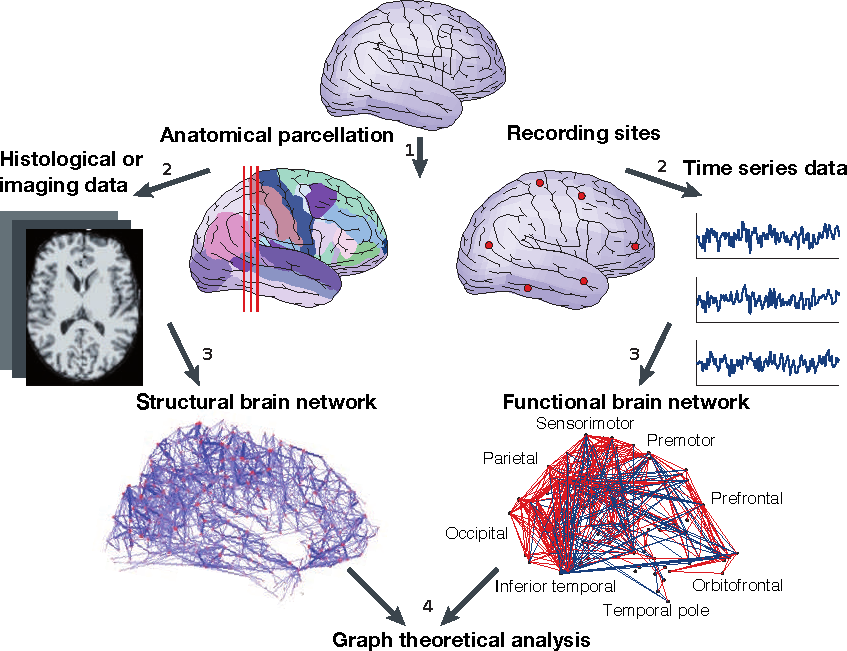
\includegraphics[width=1.0\textwidth]{images/bullmore_2009_pipeline.pdf}
\caption{Structural and functional brain networks can be explored using graph theory through four steps.
Adapted from~\cite{bullmore2009}.}
\label{fig:bullmore2009pipeline}
\end{figure}

The rise of network neuroscience in the last decade has been driven by the evidence that almost independently from how the networks links are defined, brain networks share some common features at several spatial and temporal scales.

For example, they exhibit the \emph{small-world} property~\cite{watts1998,sporns2002,sporns2004a}, whereby most nodes in a graph can be reached from any other node in just a few hops.
Small-worldness in brain networks~\cite{vandenheuvel2008} has been found to positively correlate with higher IQ in humans~\cite{vandenheuvel2009}, suggesting that human intellectual performance may be related to how efficiently our brain integrates information between multiple brain regions.

Other measures have been correlated with phenotypical and structural characteristics.
\emph{Rich-clubs} are subsets of highly connected nodes who are also highly connected to each other, forming a communication backbone.
It has been hypothesized, that rich clubs might be valuable in supporting high-level and more cognitively advanced forms of information processing~\cite{collin2014}.
Moreover, it's thought that the presence of a rich club increases the diversity of the functional repertoire over and above the effects produced by scale-freeness alone~\cite{senden2014}, a property of a network of being self-similar at different scales.
Forms of rich-club organization have been observed in cats, macaque and humans~\cite{vandenheuvel2011,harriger2012,dereus2013a,collin2014}, comprising portions of prefrontal, parietal, temporal and insular cortex.
Rich club nodes and edges participate in a large number of short paths across the network, contributing disproportionately to global communication.

From the functional point of view, central hubs of rich clubs are concentrated in heteromodal association cortices, areas that receive input from multiple unimodal sensory association areas and/or other heteromodal cortices~\cite{sporns2007,power2013,kandel2013}.
Conversely, primary sensory cortices have low topological centrality and degree~\cite{vandenheuvel2011,zamora-lopez2010,harriger2012}.
Damage to primary sensory areas only affects them locally, while perturbation to the rich-club backbone has diffuse and severe effects on the whole network architecture~\cite{honey2008,ball2014}.
Abnormal rich-club connectivity is hypothesized to be related to familial vulnerability for schizophrenia~\cite{collin2014impaired} and other diseases as well.

More generally, network neuroscience has matured the ability to map alterations at the level of structural or functional connectome and may be useful for predicting and generating hypotheses about underlying pathophysiological mechanisms of disease.
%Clinically useful predictions are now being made on the basis of network indicators, viewed as biomarkers of brain alterations~\cite{fornito2015}.
%Hence, if only a systematic biological study of the nervous system can detail the etiology of neurological diseases, their observable symptoms often result in a partial or total reorganization of the functional and structural architecture of the brain.
To this end, the definition and validation of data-driven biomarkers based on graph-theoretical observations of the effects of brain diseases is a highly desirable objective.

\section{Brain networks at the mesoscale}
Many natural and artificial networks display a modular organization, i.e. nodes group together in some kind of \emph{clusters}, resulting in a particular mesoscopic structure.
At this level of mesoscale organization, the topological properties of nodes are more dependent on their neighbourhood than on the rest of the graph.
When the structure tends to group nodes with similar properties, the mesoscale structure is called \emph{assortative}.
Graphs with an assortative structure consist of tightly connected groups of nodes that are themselves loosely connected with other groups.
These groups are therefore dubbed as \emph{communities}.

The organization into communities is one of the most studied properties of networks and a large amount of literature has grown on the topic, as reviewed in~\cite{fortunato2010}.
The problem of detecting the communities, \emph{community detection} or \emph{graph-partitioning} in the computer-science jargon, is of high theoretical and practical importance.
From the theoretic point of view, communities are representative of the generative probabilistic model underlying the formation of links~\cite{karrer2011} and tell much about the statistical properties of networks.
On the other side, practical applications of community detection are fundamental not only in neuroscience but also in sociology, computer science, biology and many other fields.
Modules derive from a decomposition of the network into subcomponents that are internally strongly coupled but externally only weakly coupled.
The property of a system of being modular or \emph{nearly-decomposable}, as already noted by Nobel prize laureate Herbert Simon~\cite{simon1991,simon1995}, helps any system to resist external perturbations by separating different functions into topologically distinct part of the system.
Near decomposability is in many respects a hallmark of complexity in natural systems~\cite{simon1991}.

Strong experimental evidence shows that the nervous system in animals and humans, from the neuronal level up to macroscopic scale, displays an organization that favours the exchange of information over a communication backbone supported by well-connected areas, the connector hubs of the network~\cite{dereus2013a}, responsible in turn for sending information to local processors, identified as the communities or modules~\cite{vandenheuvel2013a}.
Functional brain networks of humans and other animals, consist of connected subnetworks (or modules) associated with cognitive functions, of vital importance for the daily life and the interaction in the environment.
The modular organization is exhibited hierarchically at different scales, with modules inside modules.
Within this architecture that confers robustness and adaptability to the network~\cite{meunier2010}, information flows from lower level sensory cortices to higher multimodal and associative cortices~\cite{mumford1992}, thus being refined and filtered in its content at multiple stages of elaboration.
The specialized stages of neural information processing are the regions of \emph{functional segregation}, a common feature at multiple scales in the brain, from the neuronal networks to macroscopic anatomically defined regions.
From the functional point of view, segregation is meant as the statistical dependence of processing elements within the same region~\cite{tononi1994}.
\emph{Functional integration} instead is defined as significant deviation from independence of large subsystems, and is typically realized through synchronization processes that increase the statistical dependence between functional modules, a mechanism required to access widely distributed resources, needed for a coherent behaviour~\cite{tononi1998}.
A delicate balance between functional integration and segregation is realized at the edge of metastability as cortical areas are neither fully synchronized nor full desynchronized~\cite{friston1997}.


When the subtle balance between functional integration and segregation is altered, like in pathological states or for external insults, the brain responds in an adaptive manner, in order to maintain homoeostasis, where possible. The mechanisms of homoeostasis adopted are compensation, degeneracy and redundancy~\cite{fornito2015}.
Through compensation, extra neural resources are recruited to maintain normal function and thanks to neural degeneracy and redundancy~\cite{tononi1999}, it is possible for distinct regions to carry out the same function, to some extent.
When these compensatory mechanisms set in after homoeostatic perturbations, the result is a reorganization of the brain structure, involving changes in its network properties.
Among the network level changes observed after specific alterations, those relative to the brain modular structure can be investigated within the framework of complex networks science~\cite{alexander-bloch2010,alexander-bloch2012,meunier2009}.

\begin{figure}[htb!]
\centering
\hfill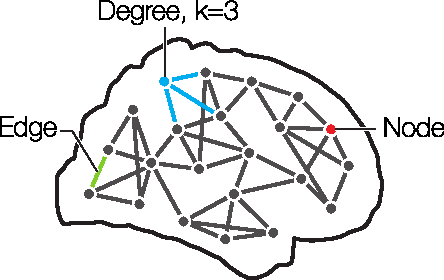
\includegraphics[height=0.25\textwidth]{images/brain_network_basics.pdf}\hfill
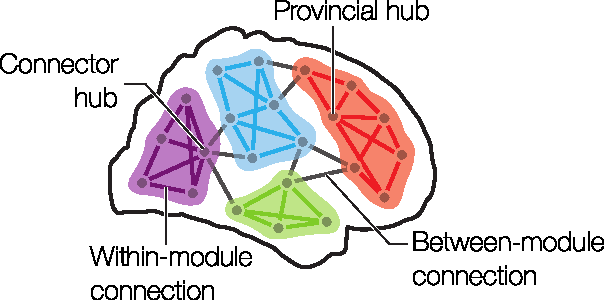
\includegraphics[height=0.25\textwidth]{images/brain_network_communities.pdf}\hfill
\caption{Meaning of communities, hubs and connectors of a brain network, depicted in an artistic view. Adapted from~\cite{sporns2016}.}
\label{fig:brain_network_communities}
\end{figure}

%This kind of structure implies that modules of heterogeneous size are present at the same time in the brain networks and that an efficient method to detect the presence of large and small modules at the same time together is in order.

Using the tools of complex network science, the evaluation of the modular structure of FC networks is cast to the problem of community detection in graphs, i.e. the problem of identifying independent groups of brain regions that exhibit strong interconnection between each other but that are weakly connected to other modules.

%% COMMENTATO DA ANGELO
% With the graph partitioned into smaller groups (or communities) of functionally connected modules, it is simpler to quantify the effect of the disease on the partitioning, as well as the areas involved in such reorganization and the role of the single nodes inside their modules.
% Indeed, an important factor when considering the effects of external perturbations on brain functioning is the degeneracy (or redundancy) of network nodes across their modules.
% Areas that are buried inside a dense module have high degeneracy, as removal of a vertex is unlikely to affect the communications between the others.
% COMMENTATO Generally speaking, poorer prognoses are registered when the interested area of the insult has low degeneracy, i.e. only that area is deputed to a particular region such that no other area may compensate.
%Severe impairments of neurocognitive functions are associated with damages to highly central nodes, as depicted qualitatively in Figure~\ref{fig:prognosis_centrality}.
% \begin{figure}[htb!]
% \centering
% 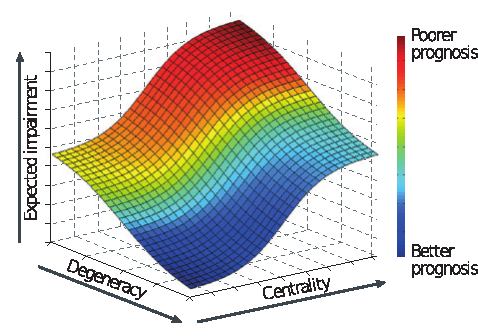
\includegraphics[width=0.75\textwidth]{images/prognosis.pdf}
% \caption{Hypothetical relation between centrality of node subjected to an pathological insult, its degeneracy and the expected functional impairment. Adapted from~\cite{fornito2015}.}
% \label{fig:prognosis_centrality}
% \end{figure}



%%%%%%%%%%%% PARTE COMMUNITY DETECTION %%%%%%%%%%%%%%%%%%%%
Several methods have been proposed to resolve the community structure of complex networks~\cite{fortunato2010,lancichinetti2009,fortunato2016}.
Many of these methods involve the definition of a fitness function that assigns positive or negative scores to edges connecting nodes within or outside the same community, and heuristics to find the optimal partition of the network that maximizes this fitness function.
Among all the methods, the most popular approach is Newman's ``Modularity maximization'' and variations thereof~\cite{newman2006}.
Following the first demonstration by~\cite{schwarz2008}, partitioning of brain networks using Newman's Modularity has been widely applied to assess the brain modular structure.
Despite its wide usage and merits, Newman's Modularity is characterized by some important limitations as it may fail to detect modules smaller than a certain scale determined by the network size, resulting in a few, relatively uniform modules of almost the same dimension.
This general behaviour, not unique to Newman's approach, is pervasive in community detection and is dubbed as \emph{resolution-limit}~\cite{fortunato2007}.

% COMMENTATO DA ANGELO The problems and drawbacks resulting from the resolution limit passed largely unnoticed in the neuroscience literature of the last years as most scientists used Newman's Modularity.
% COMMENTATO DA ANGELO This barrier has its roots in the theoretical foundations of community detection and practically implies that the detection of brain modules smaller than a scale determined by the size of the total network is very difficult, or in the worst case, even impossible.
As a consequence, even unambiguously defined modules, like almost complete sub-graphs or even cliques\footnote{Graphs where all nodes to connect to all nodes}, may be unduly merged into larger communities when they are too small compared to the size of the network.
This limit hampers the ability to detect small-scale structures of functionally correlated brain areas and to notice alterations in connectivity between subjects or groups of subjects. Hence, it mayy have prevented detection of alterations in the modular structure of brain connectivity in patients affected by various neuropsychiatric disorders
% Such limit is therefore of impediment to an implementation of a clinical-level biomarker of brain disease.
Hence, the resolution limit represents a critical shortcoming for the study of brain networks and is likely to have affected many of the studies reported in the literature.
% TROPPO SPECIFICO A QUESTO LIVELLO
%Moreover, it has been shown that an adjustable resolution parameter may reduce the tendency to merge small clusters, but only at the cost of unduly splitting large clusters~\cite{lancichinetti2011}. Adjustment of the resolution parameter is an attempt to balance these two biases, but multi-resolution methods fail to recover community structures comprising heterogeneous distributions of cluster sizes~\cite{lancichinetti2011}.

In the present work I have developed an approach that is valuable in detecting communities in brain networks beyond the resolution limit.
The following sections of this introductory chapter guide the reader into the complex networks science, by giving an overview of the mathematical terminology and methodological concepts.
In the second chapter, the experimental evidence of the modular structure of brain connectivity is reviewed, together with the methods to disentangle the mesoscopic structure of complex systems. In particular, sections~\ref{sec:resolutionlimit} and~\ref{sec:degeneracy} consider the problem of the resolution limit and degeneracy of Newman Modularity.
A new approach, dubbed Surprise, that overcomes the limitations imposed by the resolution limit and degeneracy, is described in the chapter~\ref{chap:beyondresolutionlimitbinarynetworks}.
Throughout chapters, the problems imposed by the resolution limit and degeneracy are analysed for Surprise and its weighted counterpart, Asymptotical Surprise. The characteristics of the two methods are discussed, together with an efficient algorithm aimed at their optimization.
The application of Surprise and Asymptotical Surprise to functional connectivity networks constitutes the hearth of chapters~\ref{chap:beyondresolutionlimitbinarynetworks} and \ref{chap:beyondresolutionlimitweightednetworks}, whereby the implications of a resolution limit free analysis of the functional modules are explored.
Firstly, application of Surprise reveals the presence of a rich structure of heterogeneously distributed modules, and differences in networks' partitions that are undetectable by resolution-limited methods.
An approach for the creation of realistic benchmark resting state networks is then examined.
On the ground structure provided by those networks, Asymptotical Surprise is validated and shown to outperform current resolution-limited methods.
The finer modular subdivision of resting state functional connectivity networks obtained by Asymptotical Surprise is shown to lead to substantial differences in the identification of connector hubs compared to other community detection methods.


%%%%%%%%%%%%%%%%%%%%%%%%%%%%%%%%%%%%%%%%%%%%%%%%%%%%%%%%%%%%%%%%%%%%%
%%%%%%%%%%%%%%%%%%%%%%% ELEMENTS OF GRAPH THEORY %%%%%%%%%%%%%%%%%%%%
%%%%%%%%%%%%%%%%%%%%%%%%%%%%%%%%%%%%%%%%%%%%%%%%%%%%%%%%%%%%%%%%%%%%%
\section{Elements of graph theory}\label{sec:elementsofgraphtheory}
A short and self-contained tutorial to the jargon of graph theory is in order before delving into the details of community detection and the illustration of how the resolution limit negatively affected many neuroscientific studies: this section is devoted to the introduction to the mathematical concepts of graph theory.
We adopt the typical notation used in other works of network science~\cite{newman2010book,estrada2011}.

\noindent\textbullet \,A \emph{graph} $G=(V,E)$ is a representation of a set $V$ of $n$ nodes, also called \emph{vertices}, connected by $m$ links, also called \emph{edges}, in a set $E$ (Figure~\ref{fig:simple_unweighted_graph}).

\noindent\textbullet \,A graph with no multiple links and no self-loops is dubbed \emph{simple graph}.
If multiple links exist between two nodes, the graph is called \emph{multigraph}.
Additionally, if a node links itself, the graph is called \emph{loopy graph}.
Figure~\ref{fig:loopy_multigraph} shows the combination of a multigraph and a loopy graph: a loopy multigraph.
If the direction of the links is important, the graph is called \emph{directed}, as shown in Figure~\ref{fig:directedgraph}, otherwise the graph is called \emph{undirected}.

\begin{figure}[htb!]
\centering
    \begin{subfigure}[hb]{0.4\textwidth}\centering
        \includegraphics[width=0.75\textwidth]{standalonetikz/tikz_simple_graph.tikz}
        \caption{}
        \label{fig:simple_unweighted_graph}
    \end{subfigure}
    \begin{subfigure}[hb]{0.4\textwidth}\centering
    \includegraphics[width=0.75\textwidth]{standalonetikz/tikz_weighted_graph.tikz}
    \caption{}
    \label{fig:simple_weighted_graph}
    \end{subfigure}
    \begin{subfigure}[hb]{0.4\textwidth}\centering
    \includegraphics[width=0.75\textwidth]{standalonetikz/tikz_loopy_multigraph.tikz}
    \caption{}
    \label{fig:loopy_multigraph}
    \end{subfigure}
    \begin{subfigure}[hb]{0.4\textwidth}\centering
    \includegraphics[width=0.75\textwidth]{standalonetikz/tikz_directed_graph.tikz}
    \caption{}
    \label{fig:directedgraph}
    \end{subfigure}
    \caption{Classes of graphs.
{\textbf (a)} is a simple unweighted undirected graph.
{\textbf (b)} is a simple weighted undirected graph, {\textbf (c)} is an unweighted loopy multigraph, {\textbf (d)} is a simple directed graph.}
\end{figure}

\noindent\textbullet \,The adjacency matrix $\mathbf{A}=\{A_{ij}\} \in \{0,1\}^{n \times n}$ of a binary undirected graph is a square $n\times n$ symmetric matrix with elements $A_{ij}=1$ if an edge exists between vertex $i$ and $j$ and $0$ otherwise.

\noindent\textbullet \,An \emph{edge-weighted graph} (also called weighted graph) $G=(V,E,\omega)$ is a graph that has a set of weights $\omega$ on the links (Figure~\ref{fig:simple_weighted_graph}).
Although not true in general, we consider only weighted undirected graphs with symmetrical real adjacency matrix, meaning that if an edge exists between node $i$ and $j$ the weight from $i$ to $j$ is the same as the weight from $j$ to $i$: $\omega_{ij}=\omega_{ji}$.
The weighted adjacency matrix,  indicated as $\mathbf{W}=\{ \omega_{ij} \} \in \mathbb{R}^{n\times n}$ is a real, square $n \times n$ symmetric matrix.

\noindent\textbullet \,The \emph{density} of a simple graph $\rho$ is defined as the ratio of the actual number of edges over all possible edges:
\begin{equation}
\rho = \frac{m}{\binom{n}{2}} = \frac{2m}{n(n-1)}.
\end{equation}
\noindent\textbullet \,A \emph{dense} graph is a graph where almost every possible pair of nodes is connected with an edge.
Conversely, a graph is termed \emph{sparse} if the density is low, meaning that also the adjacency matrix is sparse and the number of edges is in the order of magnitude of the number of nodes $m ~\approx \mathcal{O}(n)$.

\noindent\textbullet \,The number of edges incident to a node in a simple graph is called \emph{degree}, denoted as $k_i$.
Every half edge incident to a node is called \emph{stub}. A vertex of degree $k_i$ has therefore $k_i$ incident stubs.

\noindent\textbullet \,On simple weighted graphs, the sum of weights of the edges incident to a vertex $i$ is called \emph{strength} and is denoted as $s_i$.
Degree and strength are the sums over rows of the adjacency matrix $d_i=s_i=\sum_{j=1}^n A_{ij}$, they are equal for binary graphs, but different for weighted graphs.

\noindent\textbullet \,The \emph{degree sequence} $\{k_i\}$ $\forall i=1,\ldots,n$ is the sequence  of the degrees of the nodes, with these numbers put in ascending order, and repetitions if needed.
By the \emph{handshaking lemma}~\cite{leiserson2001}, the sum of all node degrees is equal to twice the number of links:
\begin{equation}
\label{eq:handshaking_lemma}
\sum_{i=1}^n k_i=2 |E|,
\end{equation}
consequently the \emph{average node degree} is given by
\begin{equation}
\langle  k \rangle = \frac{2m}{n}.
\end{equation}

\noindent\textbullet \,The \emph{neighborhood} of node $i$ is the set $\Gamma_i=\{j \in V | (i,j) \in E \}$.
In other words, the neighbor nodes of $i$ are the nodes which share and endpoint edge to $i$.


\noindent\textbullet \,A \emph{path} in a graph is a sequence of edges such that the destination of each edge in the sequence is always the source of the following edge.
A \emph{cycle} is a closed path, i.e.
a path where the origin and destination nodes are the same.

\noindent\textbullet \,A graph that has all the possible links, indicated by $K=(V,V\times V)$ is called \emph{complete graph} or \emph{clique} (Figure~\ref{fig:completegraph}).
Complete graphs on $n$ nodes, indicated as $K_n$ have a total of $m=\binom{n}{2}$ edges and density equal to $1$.

\noindent\textbullet \,The complementary graph $\bar{G}$ is the graph that has edges where $G$ has no edges and vice-versa, formally $\bar{G}=(V,V\times V - E)$.
The \emph{empty graph} is therefore defined as the complementary graph of the clique $\bar{K}$, as it has $n$ nodes and no edges (Figure~\ref{fig:emptygraph}).
The \emph{cycle graph} $C_n$ is a graph containing a single cycle through all nodes and is the smallest connected cyclic graph (Figure~\ref{fig:cyclegraph}).
A \emph{tree graph} is a graph with no cycles and exactly $n-1$ edges.

\noindent\begin{figure}[htb]
\centering
    \begin{subfigure}[t]{0.3\textwidth}\centering
        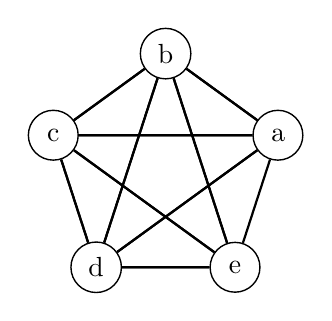
\begin{tikzpicture}
            \tikzset{LabelStyle/.style= {draw,font = \small}}
            \GraphInit[vstyle=Normal]
            \SetGraphUnit{1.5}
            \begin{scope}[rotate=18]
            \Vertices{circle}{a,b,c,d,e}
            \end{scope}
            \Edges(a,b,a,c,a,d,a,e,b,c,b,d,b,e,c,d,c,e,d,e)
        \end{tikzpicture}
    \caption{{\footnotesize Complete graph $K_5$}}\label{fig:completegraph}
    \end{subfigure}
    \begin{subfigure}[t]{0.3\textwidth}\centering
        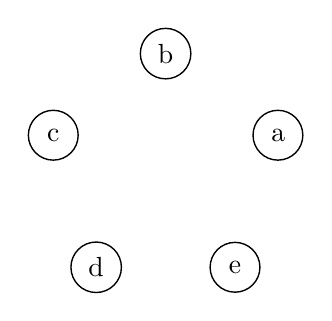
\begin{tikzpicture}
        \tikzset{LabelStyle/.style= {draw,font = \small}}
        \GraphInit[vstyle=Normal]
        \SetGraphUnit{1.5}
        \begin{scope}[rotate=18]
        \Vertices{circle}{a,b,c,d,e}
        \end{scope}
        \end{tikzpicture}
    \caption{{\footnotesize Empty graph $\bar{K}_5$}}\label{fig:emptygraph}
    \end{subfigure}
    \begin{subfigure}[t]{0.3\textwidth}\centering
        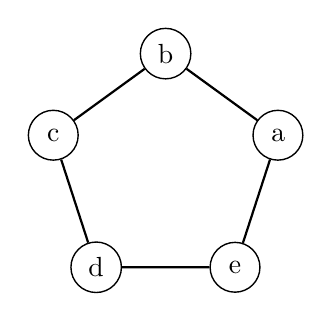
\begin{tikzpicture}
        \tikzset{LabelStyle/.style= {draw, font = \small}}
        \GraphInit[vstyle=Normal]
        \SetGraphUnit{1.5}
        \begin{scope}[rotate=18]
        \Vertices{circle}{a,b,c,d,e}
        \end{scope}
        \Edges(a,b,b,c,c,d,d,e,e,a)
    \end{tikzpicture}
    \caption{{\footnotesize Cycle graph $C_5$}}\label{fig:cyclegraph}
    \end{subfigure}
\end{figure}

\noindent\textbullet \,A subgraph $\mathcal{G}$ of a graph $G$ is said to be \emph{induced} if, for any pair of vertices $i$ and $j$ of $\mathcal{G}$, the pair $(i,j)$ is an edge of $\mathcal{G}$ if and only if $(i,j)$ is also an edge of $G$.
In other words, $\mathcal{G}$ is an induced subgraph of $G$ if it has the most edges that appear in $G$ over the same vertex set.
If $\mathcal{G}$ is chosen based on a vertex subset $S$ of $V(G)$, then $\mathcal{G}$ can be written as $G[S]$ and is said to be induced by $S$.

\noindent\textbullet \,A simple graph is said \emph{connected} if there exists a path between any pair of nodes.
If the graph itself is not connected, then it is formed by a set of connected subgraphs, also called \emph{weakly connected components}.


%%%%%%%%%%%%%%%%%%%%%%%%%%%%%%%%%%%%%%%%
\subsection{Clustering}\label{sec:clustering}
Grouping nodes according to some criterion of similarity between them is the basis of the identification of clusters in networks.

\noindent\textbullet \,A set of mutually disjoint, induced subgraphs that covers all the nodes is called a \emph{clustering}.
A clustering $\zeta = \{\zeta_c\}$ of $G$ is a partitioning of the set $V$ into $C$ disjoint sets of nodes, $\zeta_c \subseteq V$, which we call \emph{modules} or \emph{communities}, interchangeably.
Each module is a node-induced subgraph $\mathcal{G}:=(V[\zeta_c],E[\zeta_c])$, also indicated as $G[\zeta_c]$.

\noindent\textbullet \,We denote the number of nodes of the module $G[\zeta_c]$ with $n_c$, the number of edges with $m_c$ and the total number of pairs of nodes with $p_c=\binom{n_c}{2}$.
From the notational point of view, a clustering can alternatively be defined with a \emph{node assignment vector} $\sigma \in \mathbb{N}^n$ in which every node is assigned to an integer label representing the community index.


\noindent\textbullet \,The \emph{Kronecker delta} on the assignment vector $\delta(\sigma_i,\sigma_j)=1$ indicates when two nodes lie in the same module and $\delta(\sigma_i,\sigma_j)=0$ when they belongs to different modules.

\noindent\textbullet \,The \emph{internal degree} $k_{\textrm{int}}(i)$ of vertex $i$ in the module $\mathcal{G}$ is the number of edges connecting $i$ to other vertices in $\mathcal{G}$.
If $k_{\textrm{ext}}(i)=0$, the vertex has neighbors only within $\mathcal{G}$, on the other hand if $k_{\textrm{int}}(i)=0$, the vertex is disjoint from $\mathcal{G}$ and should not be part of the same community.

\noindent\textbullet \,The \emph{external} degree $k_{\textrm{ext}}(i)$ of vertex $i$ in the module $\mathcal{G}$ is the number of edges connecting $i$ to vertices not in $\mathcal{G}$.

\noindent\textbullet \,The \emph{subgraph internal degree} $K_{\textrm{int}}(\mathcal{G})$ is the sum of the internal degrees of its vertices.
Likewise, the \emph{subgraph external degree} $K_{\textrm{ext}}(\mathcal{G})$ is the sum of the external degrees of its vertices.

\noindent\textbullet \,The \emph{subgraph total degree} $k(\mathcal{G})$ is the sum of the degrees of the vertices of $\mathcal{G}$.
By definition, $K(\mathcal{G}) = K_{\textrm{ext}}(\mathcal{G}) + K_{\textrm{int}}(\mathcal{G})$.
For convenience of notation we will denote without loss of generality $K_{\textrm{int}}(\mathcal{G}[ \zeta_c ])$ as $K_c$, specifying the full notation where is needed.

\begin{figure}[htb]\centering
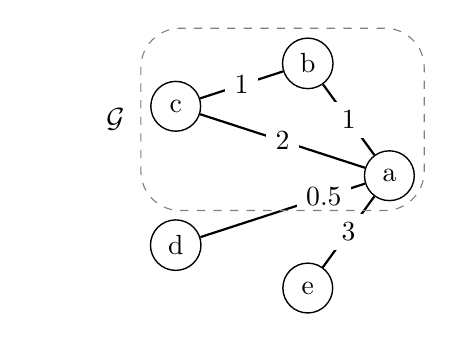
\begin{tikzpicture}
    \GraphInit[vstyle=Normal]
    \SetGraphUnit{1.5}
    \Vertices{circle}{a,b,c,d,e}
    \Edge[label=1](a)(b)
    \Edge[label=2](a)(c)
    \Edge[label=0.5,style={pos=0.25}](a)(d)
    \Edge[label=3](a)(e)
    \Edge[label=1](c)(b)
    \node[draw=black!50,dashed,rounded corners=5mm,fit=(b.north) (a.south) (c.west) (a.east)](BORD) {};
    \node[left of=BORD,anchor=east, inner sep=1cm]{$\mathcal{G}$};
\end{tikzpicture}
\caption{Internal degree $k_{\textrm{int}}(a)=2$, internal strength $s_{\textrm{\textrm{int}}}(a)=3$, external degree $k_{\textrm{ext}}(a)=2$, external strength $s_{\textrm{ext}}(a)=3.5$.}
\label{fig:internaldegree}
\end{figure}

\noindent\textbullet \,The \emph{intracluster density} of the subgraph $\mathcal{G}$ is defined as the ratio of the intracommunity edges over the number of pairs of nodes
\begin{equation}
\rho_{\textrm{int}}(G)=\frac{m_c}{p_c} = \frac{2 m_c}{n_c(n_c-1)}.
\end{equation}

\noindent\textbullet \,The \emph{inter-cluster density} is instead defined as the ratio of edges with one endpoint in $\mathcal{G}$ and the other in $G-\mathcal{G}$, over the total possible number of edges connecting $\mathcal{G}$ with the rest of the graph: 

\begin{equation}
\rho_{\textrm{ext}}=\frac{m-m_c}{n_c(n-n_c)}.
\end{equation}

\noindent\textbullet \, The total intracluster edges and total intracluster node pairs numbers are the sum over all modules $c$ of intracommunity edges and node pairs:
\begin{align}
&m_\zeta= \sum \limits_{c=1}^C |E \left[ \mathcal{G}_c \right]| = \sum \limits_{c=1}^C m_c \\
&p_\zeta= \sum \limits_{c=1}^C \binom{|V \left[ \mathcal{G}_c \right]|}{2} = \sum \limits_{c=1}^C p_c.
\end{align}

\subsection{Communities}\label{sec:communities}
The word \emph{community} applied to complex networks originated in sociology as people tend naturally to form groups: family, friends, acquaintances.
Social communities then can be thought as subgroups of people connected to each other more strongly than with other external people.

The problem of quantitatively defining a community, although intuitive at first sight, is multifaceted and ambiguous.
No universally accepted definition of network community exists and some degree of arbitrariness or common sense is required, a feature that is difficult to describe quantitatively.
Importantly, the identification of communities is possible only for relatively sparse graphs. On dense graphs indeed, the community detection problem requires different tools, closer to those of data clustering, with different concepts and definitions.

In the attempt of making the concept of community quantitative, two classes of definitions can be provided: local and global.
The \emph{local definitions} involve that a community is viewed as a separate entry or an autonomous module: the community is studied as isolated from the graph as a whole.
These definitions implies that the corresponding communities are mostly maximal subgraphs, subsets of nodes that cannot be enlarged with the addition of new nodes or edges without altering the property upon which they are defined.
The most important local criterion for communities definition are the \emph{complete-mutuality}, the \emph{reachability}, the comparison of vertex degree and \emph{internal-external cohesion}~\cite{wasserman1994,alba1973}.
Complete mutuality means that the identified community is a clique where every node is mutually connected with all the others, while reachability implies that there exist a path between every pair of nodes in the community.
The internal- external cohesion principle is equivalently represented by the Radicchi's definitions of \emph{strong communities}~\cite{radicchi2004}: for a community $\mathcal{G}$ to be defined in \emph{strong} sense, every node in the community must exhibit a larger internal degree than external degree. This concept is quantified by the following definition:
\begin{equation}\label{eq:strongcommunities}
\forall i \in V[ \mathcal{G} ] \qquad k_{\textrm{int}}(i) > k_{\textrm{ext}}(i).
\end{equation}
The strong community criterion is extremely stringent and most real-world networks, even the simplest, do not exhibit such property.
It is possible though to weaken this constraint, asking that \emph{on average} the internal degree is greater than the external degree.
Upon this idea the concept of \emph{weak communities} is built (Eq.~\ref{eq:communityweak}):
\begin{equation}\label{eq:communityweak}
\sum \limits_{i \in V[\mathcal{G}]} k_{\textrm{int}}(i) > \sum \limits_{i \in V[\mathcal{G}]} k_{\textrm{ext}}(i)
\end{equation}
Finding strong communities is more difficult than finding weak communities and most algorithms fail in this job. Most methods indeed encode their own concept of community.
Nonetheless these two last definitions are almost universally accepted and give a precise idea of the meaning of community.
Additionally, the weak criterion of community is the basis of the planted-partition model~\cite{condon2000} and its later modifications~\cite{lancichinetti2008} that we'll encounter in the next sections.

Most of the global definitions of communities encompass properties of the graph that are used by an algorithm to deliver a modular decomposition.
In this sense the global definitions are always indirect, often based on \emph{null models} or stationary properties of dynamical processes such as random walkers~\cite{pons2006,rosvall2008}.

Multiple different sub-networks in brain FC networks have been observed consistently with a variety of analysis techniques~\cite{fox2005,deluca2006,salvador2005,schwarz2007} such as ICA or other multivariate methods.
This empirical evidence, shown not only in humans but also in higher vertebrates as the cat~\cite{scannell1995} and macaque~\cite{felleman1991}, suggests that to some extent the high-level functional organization is based on the balance of two competing principles of segregation and integration.
The nervous system is obviously shaped by this balance as the need of fast information processing is satisfied by small-scale neuronal circuits, typically at the first stages of sensory input processing.
Typical examples are the very localized functional area of visual processing V1 or the primary motor cortices. At larger scale the cortex works in concert, connecting all the segregated areas in a larger, widely distributed complex network.
It is indeed more and more recognized that complex behaviours arise thanks to the dynamical interplay of the integrated and segregated actions of different regions of the brain~\cite{tononi1994,tononi1998,deco2015}.

Presence of communities within FC networks and hubs supports the concepts of integration and segregation.
Recently, experiments in which computational dynamical processes are simulated over the topology of whole-brain networks have shed light on the role of communities in shaping the cortical activity~\cite{deco2015}.
Importantly, it was found that the network communities consist in the areas that are devoted to the segregated information processing, while the hubs and rich clubs are deputed to convey that information over the whole brain.

Assessing the role of nodes within a community is an important task that depends on the community assignment. To this end one can  cartographic classification of nodal roles that describes if a node connects two communities or is buried inside its own community in of help.

\subsection{Cartographic classification of nodes}
Every node in a network is characterized by its role in relation to other nodes.
Once a clustering $\zeta$ is imposed on a graph, some nodes may act as bridges between two or more communities, having neighbours in one or the other module, others instead may share the majority of neighbours inside their same community, being more central to their module.

To investigate differences in nodal roles as determined by different community detection methods, Guimera and Amaral~\cite{guimera2005} introduced a cartographic characterization of nodes based on two parameters.
The first, dubbed \emph{participation coefficient}, indicated by $P_i$ and comprised in the range $[0,1]$ reflects the extent to which a node is connected to nodes in other modules, and is defined in Eq~\ref{eq:participationcoeff} as:
\begin{equation}\label{eq:participationcoeff}
P_i = 1 - \sum_c \left( \frac{k_{ic}}{k_i} \right)^2,
\end{equation}
where $k_{ic}$ is the number of links of node $i$ to nodes in module $c$ and $k_i$ is the total degree of node $i$.
Converselely, the second parameter dubbed \emph{within-module degree score}, indicated by $z_i$,  reflects the degree of connectivity of a node to the nodes in its same community, and is defined as: 
\begin{equation}\label{eq:withinmoduledegree}
z_i = \frac{k_i - \langle  k_{c_i} \rangle }{\sigma_{k_{c_i}}},
\end{equation}
where $\langle  k_{c_i} \rangle $ is the average degree of nodes in the same module $c$ of node $i$ and $\sigma_{k_{c_i}}$ is the standard deviation of degrees of nodes in module $c$.

Hubs classification is critical for the interpretation of the roles played by the highly connected nodes within the network structure.
The Guimera and Amaral~\cite{guimera2005} classification scheme places participation coefficient and within-module degree z-score of every node on a two dimensional plane.
Different regions of the two dimensional plane are divided empirically into seven regions as shown in Figure~\ref{fig:gagraph}.
Depending on the specific cut-off values of participation coefficient and intra-modular connectivity, the nodes are defined as ultra-peripheral (region R1), peripheral (region R2), connector non-hubs (region R3), kinless non-hubs (region R4), provincial hubs (region R5), connector hubs (region R6) and kinless hubs (region R7).
Naturally, connector hubs are of great importance for communication between modules (Figure~\ref{fig:brain_network_communities}).
Indeed, connector hubs are those with high values of participation coefficient and high values of within-module degree z-score.

In the context of brain networks, these hubs are responsible for the integration of the different modules into a cohesive structure and are thought to be particularly vulnerable in the presence of brain insult or disease, as damage to these nodes is likely to disrupt network connectedness~\cite{stam2014,fornito2015,alexander-bloch2010}.
In contrast, provincial hubs are more importantly involved in functional specialization and local processing; therefore damage to these areas may yield specific clinical deficits, whereas damage to connector hubs results in complex and pervasive neurological dysfunctions~\cite{stam2014,fornito2015}.

\begin{figure}[htb!]
\centering
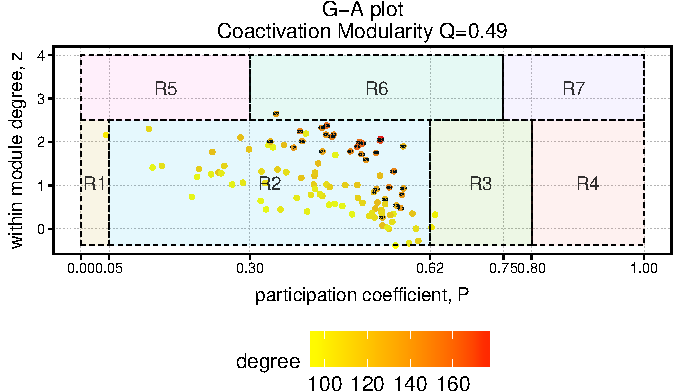
\includegraphics[width=0.75\textwidth]{images/guimera_amaral_coact_q.pdf}
\caption{Guimera and Amaral classification scheme for the modular structure induced by Modularity maximization of a co-activation network as obtained from~\cite{crossley2013a}.
Each node is indicated by specific coordinates $(P_i,z_i)$ and occupies one of the seven different regions. Nodal degrees are color-coded from yellow to red, as shown in the legend.}
\label{fig:gagraph}
\end{figure}

\begin{figure}[htb!]
\centering
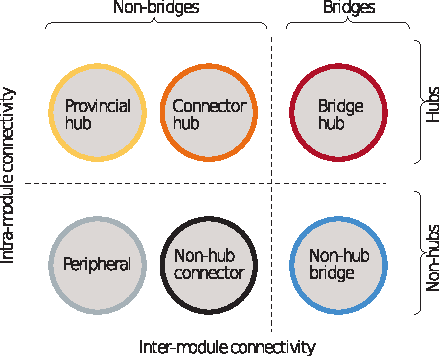
\includegraphics[width=0.5\textwidth]{images/hubs_nonhubs.pdf}
\caption{Schematic assessment of nodal roles.
Interestingly under this convention, bridges represent the most extreme case of nodes, with a relatively equal distribution of connectivity between different modules.
Hence, bridges are best detected when overlapping communities are allowed.
They bridges hubs and non-hubs occupy the R7 region of the original GA scheme.
Adapted from~\cite{fornito2015}.}
\label{fig:hubs_bridges}
\end{figure}

%%%%%%%%%%%%%%%%%%%%%%%%%%%%%%%%%%%%%%%%%%%%%%%%%%%%%%%%%%%%%%%%%%%%%
%%%%%%%%%%%%%%%%%%%%%% Models of random graphs %%%%%%%%%%%%%%%%%%%%%%
%%%%%%%%%%%%%%%%%%%%%%%%%%%%%%%%%%%%%%%%%%%%%%%%%%%%%%%%%%%%%%%%%%%%%

\subsection{Models of random graphs}\label{sec:models_random_graph}
A large effort of network science is devoted to the description of the generative processes that lead to the networks observed in real-world settings.
The ability to understand such generative models is of primary importance in many fields, as it enables researchers to make predictions about the behaviour of the system under exam and to compare systems, gaining knowledge.
In general, a random graph is a model network in which some specific set of parameters take fixed values, but the network is random in other respects.
The theory of random graphs studies the intersection between graph theory and probability theory.
%In the first part of the twentieth century, mathematicians developed advanced theories of random graphs as they needed to compare the properties of real-world networks against random null hypotheses.
%A random graph is a probability space $(\Omega,\mathcal{F},\mathcal{P})$, where the sample space $\Omega$ is a nonempty set of graphs, the set of events $\mathcal{F}$ is a collection of subsets of the sample space (usually the power set of $\Omega$), and $\mathcal{P}$ is a function that assigns a probability to each event.
It is usual to describe a random graph by a sequence of steps to construct it. This sequence is called a \emph{random graph model}.

%Given the unavailability of computer simulations at that time, the simplest model dates back to 1959 and is due to Erd\H{o}s and Rényi~\cite{erdos1959}.
In the Erd\H{o}s-Rényi model (also called $G_{n,m}$ model, the sample space $\Omega$ is the set of all graphs having $n$ nodes and $m$ edges.
One of the simplest models is the random network generated by selecting exactly $m$ edges from the set of all possible edges and placing them at random over the nodes pairs.
This model, with the fixed constraint of edge number, is mathematically known as $G(n,m)$ or \emph{Gilbert} random graph.
In probabilistic terms, the $G(n,m)$ graph is equivalent to say that the network is sampled choosing uniformly from the set $\Omega$ of all $\binom{\binom{n}{2}}{m}$ possible graphs.
Intuitively then it is possible to assign a probability score to each instance of a random graph model.
In the $G(n,m)$, each instance is equiprobable.

Strictly speaking, a random graph model is better defined as an ensemble of networks, therefore as a probability distribution $\mathcal{P}(\Omega)$ over the space of all graphs $G$.
TThe Gilbert random graph model is associated with a probability distribution sharply peaked in $\mathcal{P}(G)=1/\Omega$ for graphs with $n$ nodes and exactly $m$ edges, and zero otherwise.
Although some properties of the $G(n,m)$ models are easy to compute, like the mean number of edges (trivial), others are more complicated because of the hard constraint imposed on edge number.

A way more useful random graph model is instead due to Erd\H{o}s and Rényi~\cite{erdos1959}.
To solve the analytical computation problems on the $G(n,m)$ model, the Erd\H{o}s-Rényi model introduces a parameter $p_{\textrm{er}}$ that specifies the probability for an edge to exist given two nodes, rather than picking exactly $m$ edges.
Technically the $G(n,p)$ random graph model or \emph{Erd\H{o}s and Rényi} (ER) model, is the ensemble of simple graphs with $n$ nodes in which each simple graph $G$ of $m$ edges appears with probability
\begin{equation}
P(G)={p}_{\textrm{er}}^{m}(1-p_{\textrm{er}})^{\binom{n}{2}-m}
\end{equation}
Differently from the $G(n,m)$ model, because of the Bernoulli distribution of edges, this graph model is also called \emph{Bernoulli random graph} or \emph{Poissonian random graph} and generally intended as \emph{the} random graph.

As every graph obtained from the Erd\H{o}s-Rényi model is a sample from a probability space, a description in terms of ensemble averages is more appropriate.
In the ER model, the expected number of edges in such a graph is the average over $\binom{n}{2}$ independent coin tosses with probability $p_{\textrm{er}}$, namely $\langle  m  \rangle = \binom{n}{2}p_{\textrm{er}}$ and the expected degree $\langle  k \rangle = p_{\textrm{er}}(n-1)$ is the same for every node.
The probability that a node $i$, chosen at random, has degree $k$ is called the \emph{degree distribution}.
In general terms, such probability is expressed as:
\begin{equation}
\Pr(k) = \frac{\langle  |\{ i \| k_i=k \}| \rangle }{n}.
\end{equation}
In the ER model, a given node is connected with probability $p_{\textrm{er}}$ to each of the other $n-1$ nodes.
Hence, the probability of being connected to a particular $k$ other nodes and not to any of the others is $p^k(1-p)^{n-1-k}$, but since there are $\binom{n-1}{k}$ ways to choose those $k$ other nodes, hence the total probability of being connected to exactly $k$ others is:
\begin{equation}
\Pr(k) = \binom{n-1}{k}p_{\textrm{er}}^k(1-p_{\textrm{er}})^{n-1-k}
\end{equation}
a binomial distribution that can be approximated to a Poisson distribution for large $n$:
\begin{equation}
\Pr(k) \approx \frac{(n \, p_{\textrm{er}})^k e^{-n \, p_{\textrm{er}}} }{k!}.
\end{equation}
\bigbreak
In generalizing the concepts of random networks models, one can define every simple graph on $n$ nodes as the output of a random process where each edge $(i,j) $ is sampled with a probability $\Pr(i,j)_{ \boldsymbol \theta}$ with $\boldsymbol \theta$ a vector of hyperparameters.
In the simplest case of the ER graph, this generative model is an uniform probability distribution with $\boldsymbol \theta=p_{\textrm{er}}$ as every pair of nodes is linked by an edge with constant probability.

Importantly, both the ER and Gilbert models should not exhibit any modular structure as every substructure that appears is an effect of random fluctuations due to finite sampling effects. Nonetheless, some algorithms may find communities in ER graphs, due to overfitting~\cite{guimera2004}.
Additionally, the ER model does not realistically represent empirical networks, even if it is very useful to simplify analytical calculation of network properties.
Its Poissonian degree distribution (Figure~\ref{fig:deg_dist_poisson_er}) is far from the degree distributions seen in most of the real-world networks.
In fact, the empirical behaviour of the degree distribution of real networks is one of the main reasons why they attracted so much interest from the scientific community.

The world-wide-web, as well as the connectome of the worm \emph{C.
Elegans}\footnote{\emph{Caenorbiditis elegans}, a small nematode worm, famous as the first living organism whose connectome has been completely mapped.} and many other examples, shows that the degree distribution of complex networks is not centered around a mean value, as predicted by ER model, instead highly connected nodes exist within a bulk of low connected nodes and the degree distribution is not decaying exponentially, thus producing the observed phenomenon of \emph{heavy tails}.
\begin{figure}
\centering
\begin{minipage}[b]{0.5\textwidth}\centering
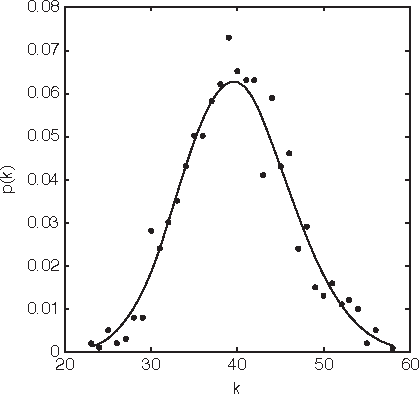
\includegraphics[height=4cm]{images/deg_dist_poisson_er.pdf}
\end{minipage}\noindent
\begin{minipage}[b]{0.5\textwidth}\centering
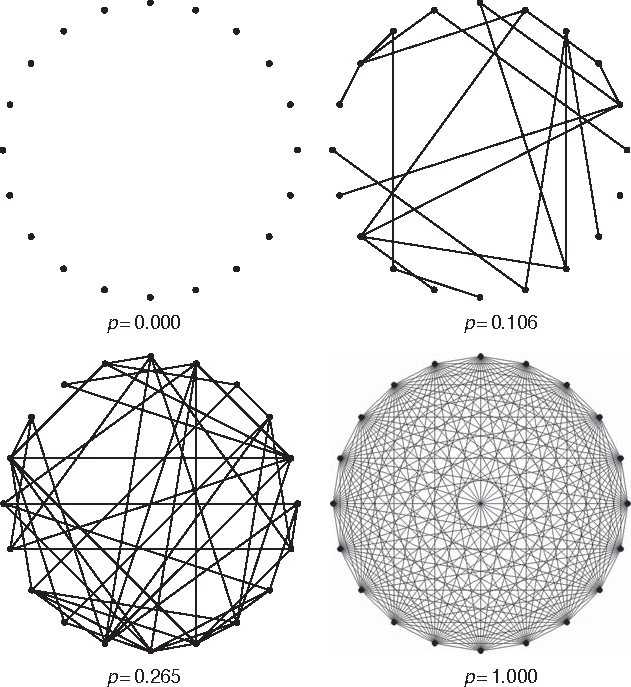
\includegraphics[height=4cm]{images/er_graphs.pdf}
\end{minipage}
\caption{Examples of ER graphs.
On the left the Poisson degree distribution of an ER network, $n=1000$,$p=0.04$.
On the right ER model instances at different values of $p$.
Adapted from~\cite{estrada2011}.}
\label{fig:deg_dist_poisson_er}
\end{figure}
Many networks display a degree distribution that follows a \emph{power-law} form:
\begin{equation}
\Pr(k) \propto k^{-\gamma}
\end{equation}
where $\gamma$ is usually included in the $[2,3]$ interval.
Power-law distributions, also dubbed \emph{scale-free}, lack a specific scale.
Indeed, $P(\alpha k)=f(\alpha)P(k)$ for some multiplicative constant $\alpha$  and $f$ a function of $\alpha$.
Therefore, the functional form of the power-law remain unchanged.

Hence, in understanding the limitation of the Erd\H{o}s-Rényi model, researchers developed a multitude of generative models of graphs that tried to better model properties like the heavy-tails saw in power-laws or also the \emph{small-worldness} phenomenon, i.e.
the observation that most nodes in a network are reachable from every other in a small number of hops.
To keep into account the features of empirical networks, other models of networks have been developed like the models of Watts-Strogatz~\cite{watts1998} model and Barabasi-Albert~\cite{barabasi1999}.

For example, in the Watts-Strogatz model a graph with groups of densely connected nodes is generated as follows:
\begin{enumerate}
\item Construct a ring with $n$ nodes and connect each node to the $l$ nearest nodes ($l/2$ nodes on each side of the ring).
\item Choose a node $i$ and the edge $e$ that connects $i$ to its nearest neighbour in a clockwise manner.
\item With probability $p_r$ replace the edge $e$ by the edge that connects $i$ to a node taken at random according to a uniform distribution over the entire ring.
\item Repeat the steps 2 and 3 for each node in clockwise manner.
\item Choose a node $i$ and the edge $e$ that connects $i$ to its second neighbour in a clockwise sense and repeat the steps 2-4.
\item Repeat the process considering the third nearest neighbour and so on until each edge of the original lattice has been considered.
\end{enumerate}

The resulting graph shows the property of having short average path length, although the degree distribution is not power-law.
To prevent this issue, the Barabasi-Albert graph model aims to construct graphs with a dynamic attachment process.
In the BA model, one considers a small number $n_0$ of initial nodes.
Then at each step, one adds a new node and connect it to a fixed number $(\leq n_0)$ of nodes that already exist in the network.
The probability that the new node will be connected to a node $i$ is then proportional to $k_i^{p_s}$,  where $p_s$ is a parameter called the \emph{scaling exponent}.
That algorithm generates graphs in which the frequency of nodes with degree $k$ is asymptotically proportional to ${k}^{-3}$.
This power relationship between frequencies and degrees indicates that this model accounts for the power-law distribution of degrees seen in many real networks.
Although very well studied, both models are still lacking a strong community structure and more complex models have been studied to explicitly embed modules.

\subsection{Stochastic block models}\label{sec:sbm}
None of the previously reported generative models explicitly accounts for the modular structure.
The modules often observed in the ER model are due to statistical fluctuations.
The BA model, too, does not take into account a block structure, when generating a power-law network and clusters in the BA model are due to local structures around nodes with high degree.
To overcome these limitations, a variable encoding the block structure must be taken into account explicitly.

The most commonly used generative model for random modular networks is called the stochastic block model (SBM)~\cite{holland1983}, which generalizes the Erd\H{o}s-Rényi random graph by giving each pair of nodes a connection probability depending only on their module affiliation $\boldsymbol \sigma$.
The SBM model tends to produce graphs containing communities, subsets characterized by being connected with one another with specific edge densities.

A stochastic block model for undirected graphs is defined by three variables: the number of nodes $n$, the set of communities (represented by a membership vector $\boldsymbol \sigma$) and a symmetric square matrix  $\mathbf{B} \in \mathbb{R}^{|C| \times |C|}$ of edge probabilities between modules.
In the case the matrix $\mathbf{B}$ is constant, the SBM recovers exactly the ER model.
If the matrix $\mathbf{B}$ takes only two different values, a model known as the \emph{planted partition model}, each pair of nodes in the same block are connected with probability $\mathbf{B}_{ij}=p_{in}$ and pairs of nodes in different modules are linked with probability $\mathbf{B}_{ij}=p_{out}$, as shown in Figure~\ref{fig:planted_peixoto}.
Specific edge probability in the planted partition model is simply described as $\Pr_{ij} = p_{in}\delta(\sigma_i,\sigma_j) + p_{out}(1-\delta(\sigma_i,\sigma_j))$.
In building the planted partition model, though one has to set in advance the number of modules $|C|$ (or blocks) and to define an equal number of nodes in every module.

\begin{figure}[htb!]
\centering
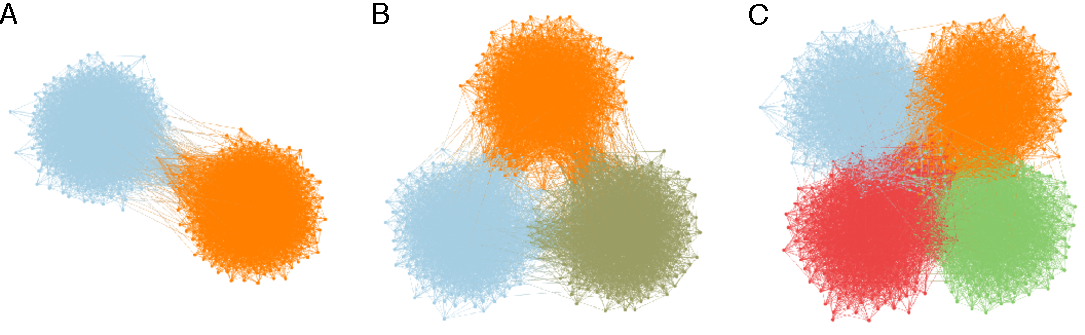
\includegraphics[width=1.0\textwidth]{images/peixoto_block_models.pdf}
\caption{Realizations of the planted partition model with different intra- and extracluster linking probabilities and number of modules.
A., $|C|=2, p_{in}=0.99, p_{out}=0.025$, B.
$|C|=3, p_{in}=0.98, p_{out}=0.06$, C.
$|C|=4 p_{in}=0.97, p_{out}=0.12$.
Adapted from~\cite{peixoto2015}.}
\label{fig:planted_peixoto}
\end{figure}

Although largely used, the planted-partition model has several drawbacks.
Indeed, as a generalization of the ER model, each node has the same expected degree and all communities have the same size.
While, these properties are of great help when performing analytical calculations, they also make it badly suited for practical applications, as degree homogeneity is seldom realized in real networks.

To overcome the unrealistic settings of the planted partition model, the Lancichinetti\hyp{}Fortunato\hyp{}Radicchi (LFR) model, first described in~\cite{lancichinetti2008}, modified the planted partition model to exhibit power-law distribution of both node degrees and community size, with tunable exponents $\tau_d$ and $\tau_c$ respectively, to respect what is observed in real networks.
As each realization is accompanied by the membership affiliation vector $\boldsymbol \sigma$, the LFR model has been used primarily as a benchmark for evaluating the effectiveness of different community detection methods~\cite{fortunato2010,lancichinetti2009} at different levels of difficulty.
Furthermore, the LFR model was extended to weighted networks with possibly overlapping modules in~\cite{lancichinetti2009a}.
The major advantage of the LFR model is the tunable level of community mixing.
Indeed, each node share a fraction $1-\mu_t$ of edges with nodes in its same community and a fraction $\mu_t$ with nodes in other communities: $0 \leq \mu_t \leq 1$ is dubbed the \emph{topological mixing parameter}.
Additionally on weighted networks, a parameter $\beta$ is used to assign strength to each node: $s_i=k_i^\beta$.
This power-law form of node strengths is chosen to match observations on real graphs, as indicated by~\cite{barrat2004}.
A weights-mixing coefficient $\mu_w$ is used to divide the node strength into two components, intra- and inter community, such that:
$$s_i = (1-\mu_w)s_i^{(intra)} + (\mu_w)s_i^{(inter)}.$$

The actual weights of the edges are then chosen to minimize the variance between the expected and the observed strengths by means of an iterative optimization step.
Hence is possible to obtain a theoretical estimate of the average edge weights that reads:
\begin{align}
\langle  w^{int} \rangle &= \frac{(1-\mu_w)\langle  s\rangle }{(1-\mu_t)}\langle  k\rangle = \frac{(1-\mu_w)}{(1-\mu_t)}\langle  k \rangle ^{\beta-1}, \\
\langle  w^{ext} \rangle &= \frac{(\mu_w)\langle  s\rangle }{(\mu_t)}\langle  k\rangle = \frac{(\mu_w)}{(\mu_t)}\langle  k \rangle ^{\beta-1}.
\end{align}
For the planted partition model, communities were defined as long as $p_{in}>p_{out}$. For the weighted LFR model instead the condition to have well defined communities is:
\begin{equation}\label{eq:wintwextflr}
\langle  w^{int} \rangle \geq \langle  w^{ext} \rangle 
\end{equation}
resulting in the equivalent formulation $\mu_w  \geq \mu_t$.
If condition~\ref{eq:wintwextflr} is not met, then each node has on average a strength relatively higher than its degree, an unrealistic circumstance in real-networks, as highest degree nodes are typically nodes with high strength~\cite{barrat2004}.

The modularity of the LFR network is controlled primarily by the topological mixing coefficient.
In the case $\mu_t$ is exactly zero, the network consists of isolated components and the stochastic block matrix is completely assortative or block-diagonal.
Conversely, for $\mu_t=1$, the block matrix is null on the diagonal and completely disassortative, exhibiting no links inside communities and only links between them.
The LFR model has a number of other parameters that control all the network parameters with great precision~\cite{lancichinetti2008,lancichinetti2009a} as described in Figure~\ref{tab:lfrparams}.
The LFR model is of great importance as it served as a benchmark test for community detection algorithms and as a model of heterogeneity of modules size when studying the performance of community detection methods. The original c++ code to generate LFR weighted networks is available at the Santo Fortunato's homepage~\url{https://sites.google.com/site/santofortunato/package3.tar.gz}.
Bindings for \texttt{Matlab,Octave} and \texttt{Python} the Fortunato's code are freely available at~\url{https://github.com/carlonicolini/lfrwmx}.

\begin{figure}[htb!]\centering
	\begin{footnotesize}
		\begin{minipage}[b!]{0.5\textwidth}
			\begin{tabular}{l p{0.98\textwidth}}
			$\tau_d \geq 1$ & Power-law exponent of nodes degrees.\\
			$\tau_c \geq 1$ & Power-law exponent of community size.\\
			$\beta \geq 1$  &Exponential parameter for strengths distribution.\\
			$C \in [0,1]$ & Desidered average clustering coefficient.\\
			$\min_c$ & Minimum number of nodes in each community.\\
			$\max_c$  & Maximum number of nodes in each community.\\
			$\mu_t \in [0,1]$ & Topological mixing coefficient.\\
			$\mu_w \in [0,1]$ & Weights mixing coefficient.\\
			$\langle k\rangle $ &Desidered average degree.\\
			\end{tabular}
		\end{minipage}\hfill
		\begin{minipage}[b!]{0.35\textwidth}\flushright
			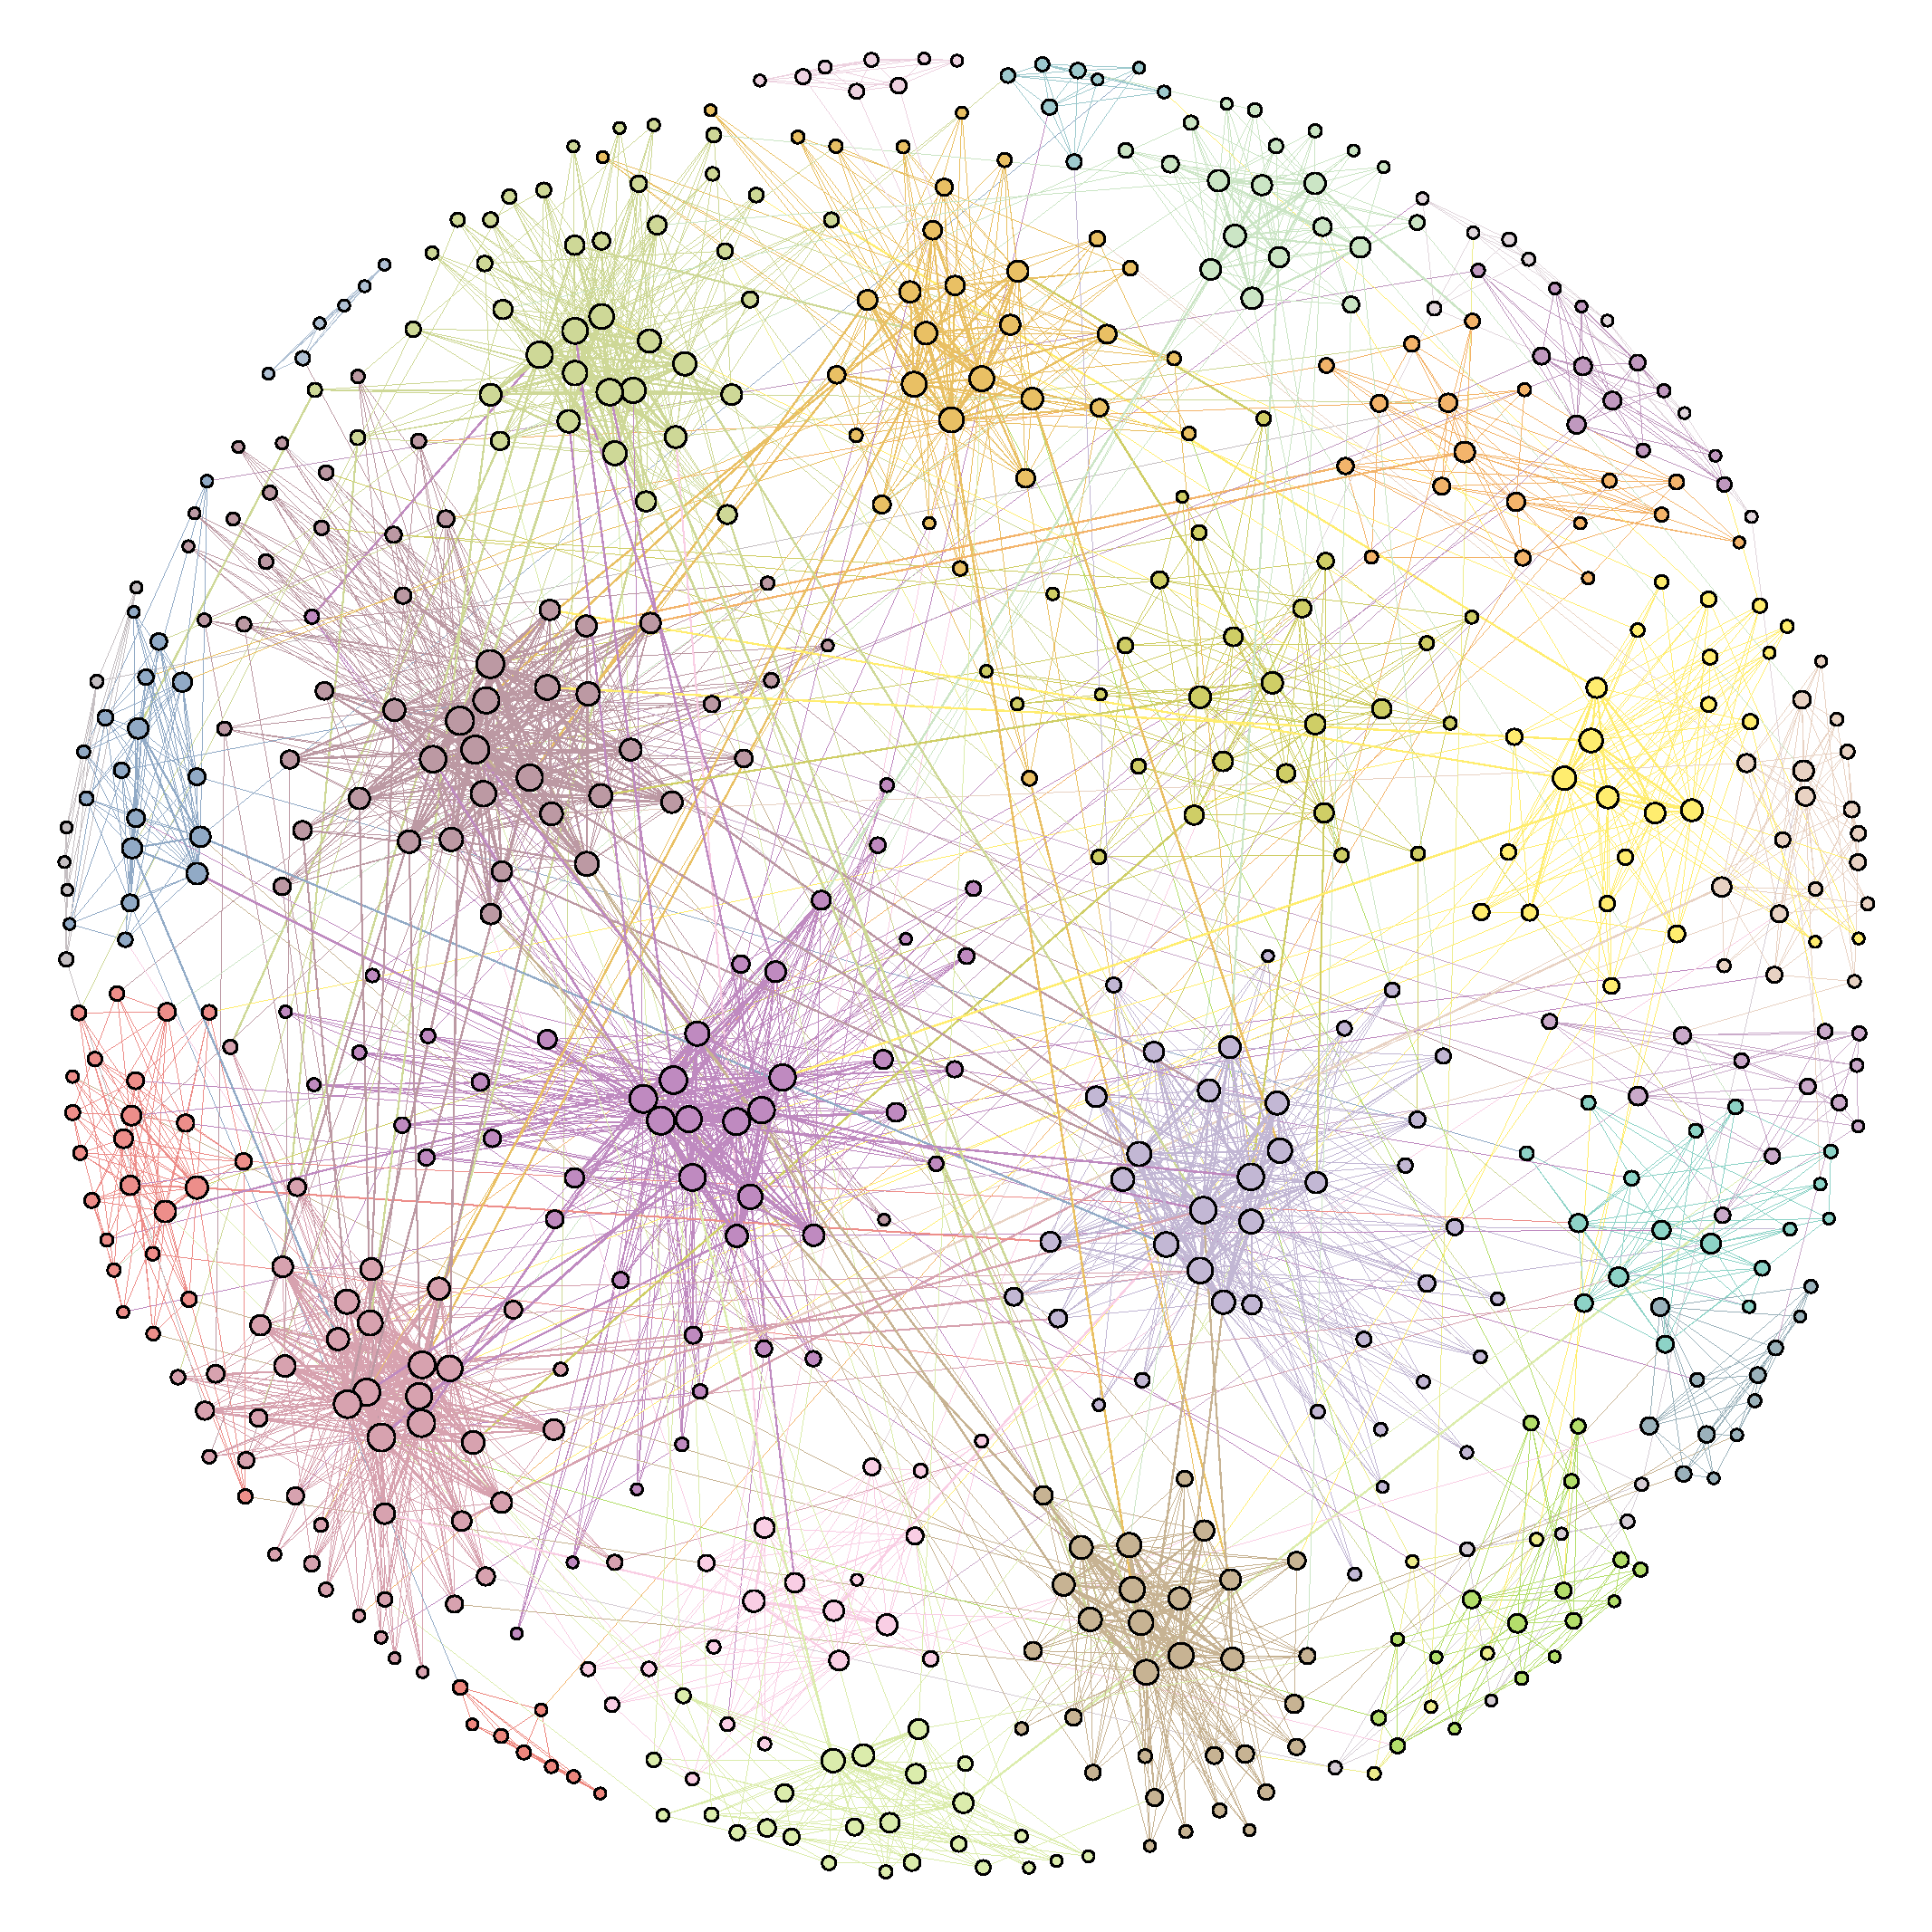
\includegraphics[width=1\textwidth]{images/LFRexample.pdf}
		\end{minipage}
	\end{footnotesize}
	\caption{LFR parameters and a single instance with $n=600$, $\langle k \rangle =12$, $\tau_d=2$, $\tau_c=1$, $\mu_t=0.1$, $\mu_w=0.1$, $\min_c=5$, $\max_c=50$.}
	\label{tab:lfrparams}
\end{figure}


% \subsection{Power law ring of cliques}
% The modified ring of clique network as indicated in the main text is composed by a ring structure of cliques whose sizes are randomly sampled from a power-law distribution with exponent $\tau_c=1$.

% The power-law distribution of sizes of cliques in this benchmark is consistent with the heterogeneous size of modules observed in brain connectivity using the binary version of Surprise.
% An example realization of the benchmark network is shown in Figure \ref{fig:ring_of_clique_powerlaw}.
% \begin{figure}[htb]
\centering
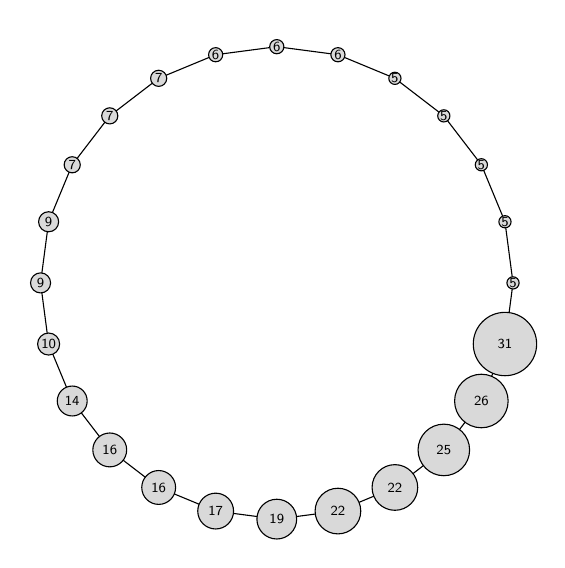
\begin{tikzpicture}
\def\cradius{3.0};
%\draw[help lines,step=1] (0,-5) grid (10,5);
\edef\counter{0};
%\def\sizes{{ 4, 4, 4, 9, 15, 17, 45, 52}};
\def\sizes{{5, 5, 5, 5, 5, 6, 6, 6, 7, 7, 7, 9, 9, 10, 14, 16, 16, 17, 19, 22, 22, 25, 26, 31}};

\draw (0:\cradius)
\foreach \x in {0,15,...,345}{ -- (\x:\cradius) }-- cycle (90:\cradius) node[above] {};

\foreach \angle in {0,15,...,345}{
      \def\cliquer{ {\angle * 0.002} };
      
      \pgfmathsetmacro{\pg}{\sizes[\counter]}; % set the macro pg with the current value of counter
      \counter
      \fill[draw, fill=gray!30] (\angle:\cradius) circle (\pg * 0.0125+0.015);
      %\draw[fill=gray!30] (\angle:\cradius) circle [radius=0.1];
      \node[black] at (\angle:3) {{\tiny $\mathsf{{\pg}}$}};
      \pgfmathparse{\counter + 1}; \xdef\counter{\pgfmathresult}; % increment counter and store the result again in counter
      }
\end{tikzpicture}
\caption{Power-law ring of cliques. Every circle is a complete graph (clique). Every clique is connected to its neighbors with one single link. The sizes of the cliques are randomly sampled from a power-law distribution with minimum clique size $\min_c=5$, maximum clique size $\max_c=75$, $n=150$, $\tau_c=1$.}
\label{fig:ring_of_clique_powerlaw}
\end{figure}

%%%%%%%%%%%%%%%%%%%%%%%%%%%%%%%%%%%%%%%%%%%%%%%%%%%%%%%%%%%%%%%%%%
%%%%%%%%%%%%%%%%%%%%%%%%%%%%%%%%%%%%%%%%%%%%%%%%%%%%%%%%%%%%%%%%%%

\section{A synthetic model of a resting state network}
Among the synthetic generative models for complex networks, no model tries to embed the typical circumstances that take place when measuring human brain resting state activity with fMRI.
To this end, here I introduce a theoretically sound method for the generation of synthetic FC networks that mimic properties of resting state fMRI networks, including noise and intersubject variability, while presenting a pre-determined ground-truth modular structure against which the performance of community detection algorithms can be tested~\cite{nicolini2017}.

The general idea is that, starting from an adjacency matrix with a given modular structure, we can generate time-courses for each of the nodes whose pairwise correlations reproduce the edge structure of the original matrix. Noise can be added to the time-courses, and the resulting correlation matrix will provide a noisy representation of the original one. This procedure can be repeated multiple times to produce different datasets that represent different subjects in the study.

In practical terms, given an undirected weighted graph  $\mathbf{C} \in \mathbb{R}^{n\times n}$ whose community structure is known a-priori, its nearest positive definite matrix~\cite{Higham1988} is obtained with its Cholesky decomposition, i.e. an upper triangular matrix $\mathbf{L}\in \mathbb{R}^{n\times n}$ such that $\mathbf{L}\mathbf{L}^T=\mathbf{C}$.
Starting from uncorrelated variables $\mathbf{X} \in \mathbb{R}^{n \times l}$, one can then generate correlated random variables $\mathbf{Y}=\mathbf{L} \mathbf{X}$ such that $\mathbb{E}(\mathbf{Y}\mathbf{Y}^T)=\mathbf{C}$ \footnote{Since the covariance matrix of a zero-mean, unit-variance random variable $X$ is given by $\mathbb{E}(XX^T)$, it's easy to verify that $\mathbb{E}(YY^T)=\mathbb{E}(LX)(LX)^T=\mathbb{E}(LX)X^T L^T=L\mathbb{E}(XX^T)L^T=L^T\mathbf{I}L=C$}.
Different levels of noise can then be injected into $\mathbf{Y}$ prior to the computation of the correlation matrix.
Schematic of this procedure is shown in Figure~\ref{fig:flowchart}.
As described in~\cite{nicolini2017} I tested this idea on two different models of planted partition: a variant of the ring of cliques~\cite{fortunato2007} and the Lancichinetti-Fortunato-Radicchi (LFR) network~\cite{lancichinetti2008}, whose degree distribution and modular structure can be tuned to replicate topological features of real-world networks, including scale freeness~\cite{hagmann2008} and the presence of densely interconnected cores~\cite{vandenheuvel2011}.

\begin{figure}[htb!]
\centering
%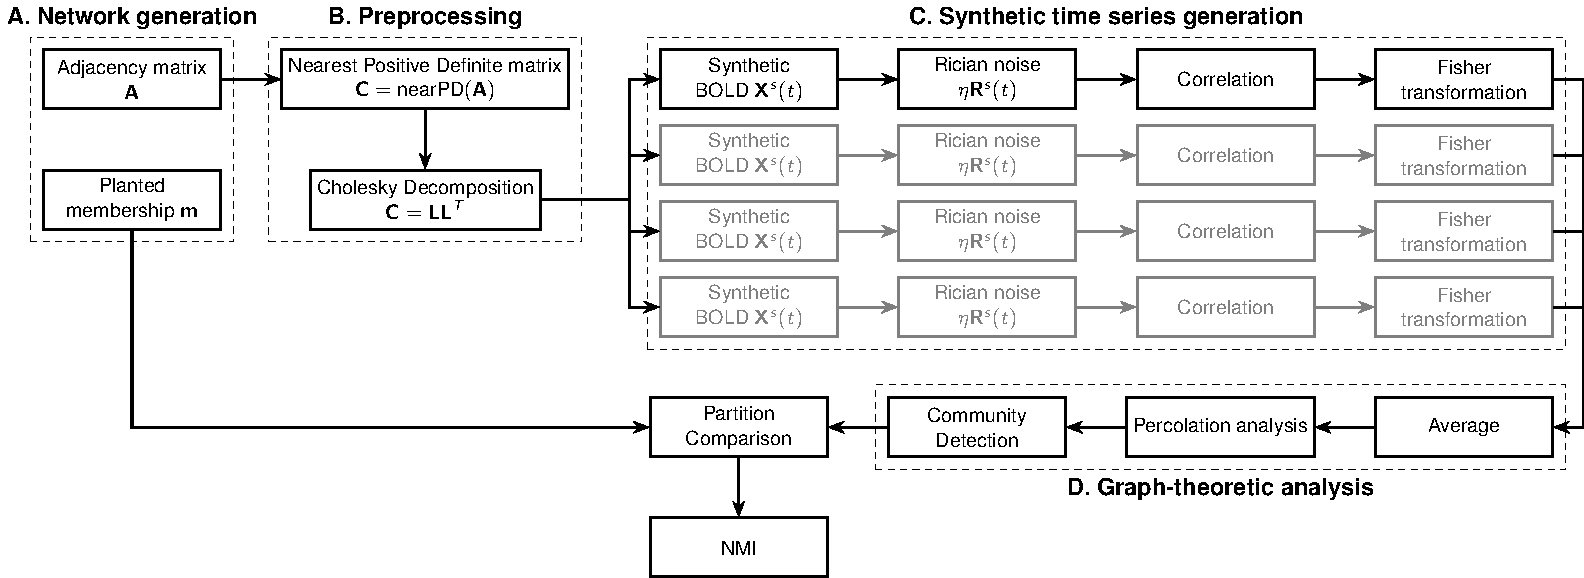
\includegraphics[height=0.25\textheight]{images/flowchart.pdf}
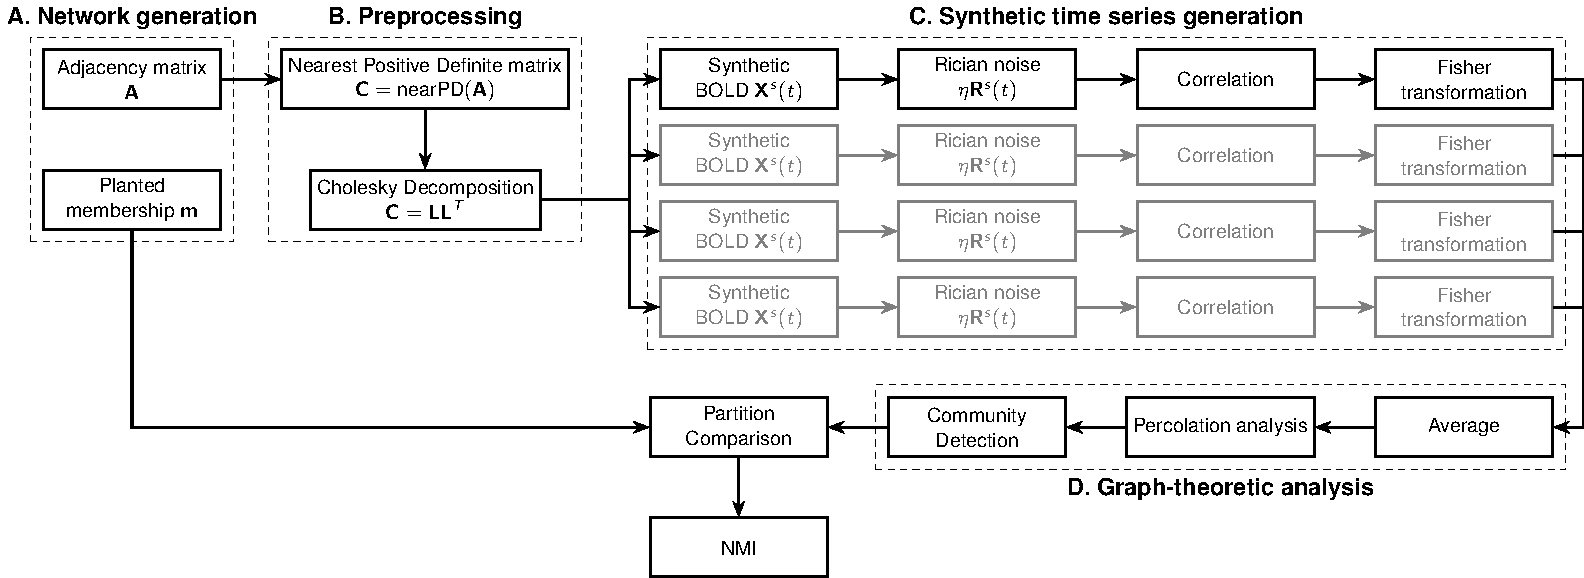
\includegraphics[width=\textwidth]{images/flowchart.pdf}
\caption{Flowchart of the generation and analysis of the synthetic datasets. In A the network with a pre-defined community structure is generated. The adjacency matrix is then processed in block B to obtain the nearest positive definite matrix for the Cholesky decomposition. This enables the generation of node-wise time-courses into which different levels of noise can be injected. The procedure is repeated multiple times to generate different instances (mimicking different subjects in the sample). Finally, correlation matrices are calculated for each instance (block C), and Fisher transformed to calculate the average adjacency matrix for analysis by community detection algorithms (block D). Lastly, resulting partitions are compared with the original, planted one in terms of NMI.}
\label{fig:flowchart}
\end{figure}

%%%%%%%%%%%%% COMPARING COMMUNITY STRUCTURE IN NETWORKS %%%%%%%%%%
\section{Comparing community structure in networks}
As the number of community detection methods has increased over the years, a quantitative way to assess their performance is desirable.
In generative models of networks like the stochastic block model and its variants, the planted partition model and the LFR benchmark, the community structure is determined a-priori.
Conversely, community structures of real-world networks are often annotated by experts in the field, like for instance the karate club network of Zachary~\cite{zachary1977} and the political blog network~\cite{adamic2005}, as no a-priori structure was imposed to those graphs.

A large number of functions for comparing similarities and differences between partitions of a network have been proposed in the past~\cite{danon2005,vinh2010}.
They are used to provide quantitatively a number that tells the extent of similarity between two partitions.
Typically the result is normalized in the $[0,1]$ range, being close to $1$ for very similar clusterings and close to $0$ when mostly dissimilar.
%These metrics are adopted especially in the benchmarking of community detection methods when the specific outcome of some algorithm is compared with a ground truth partition, usually, a-priori determined.

The most well-grounded and performing metrics for the comparison of two community structures are rooted in information theory~\cite{danon2005,vinh2010,cover2006}.
\emph{Normalized Mutual Information}~\cite{danon2005} and \emph{Variation of Information}~\cite{meila2007} are the most widely used, despite it was recently found that both of them suffer from systematic errors due to the finite size of the network~\cite{zhang2015a}.
In the rest of the discussions, we ignore the limitation of finite size effects, by only working with relatively large networks.

Normalized Mutual Information (NMI) assumes that the clustering comparison is a problem of message decoding.
Implicit in this interpretation is the idea that if two partitions are similar, inferring one partition from the other needs very little information.
Let us denote two generic partitions of the same graph by their clusterings $\zeta^x,\zeta^y$ with $c_x$ and $c_y$ communities respectively: $\zeta^x=\{\zeta^x_1,\ldots,\zeta^x_{c_x}\}$ and $\zeta^y=\{\zeta^y_1,\ldots,\zeta^y_{c_y}\}$.
The number of nodes in the $i$-th community of $\zeta^x$ is $n_i :=|\zeta^x_i|$ and the number of nodes in the $j$-th community of $\zeta^y$ is $n_j:=|\zeta^y_j|$.
The two communities share a number of nodes $n_{ij}=| \zeta^x_i \cap \zeta^y_j|$.
Let us also consider the community assignments $\boldsymbol\sigma^x_i$ and $\boldsymbol\sigma^y_i$ for partitions $\zeta^x$ and $\zeta^y$ respectively; we treat the labels as values of two random variables $X$ and $Y$ with joint distribution $P(x,y)=P(X=x, Y=y) = n_{xy}/n$, which implies that $P(x)=P(X=x)=n_x^X/n$ and $P(y)=P(Y=y)=n_y^Y/n$.

The \emph{mutual information} between the two clusterings $\zeta^x,\zeta^y$ is then defined as $I(X,Y)=H(X) - H(X|Y)$ where $H(X)=-\sum_x p(x) \log p(x)$ is the Shannon entropy of $X$~\cite{cover2006}.
The mutual information itself is not very useful, because hierarchically splitting the clusters in $\zeta^x$ would produce no change in the prior $H(X|Y)$ and partitions with different hierarchies of the same clusters, would go unnoticed.
This observation led Danon~\cite{danon2005} to introduce normalized mutual information for clustering comparison as: 
\begin{equation}\label{eq:nmi}
\textrm{NMI}(X,Y) = \frac{2I(X,Y)}{H(X)+H(Y)} = \dfrac{2\sum \limits_{i=1}^{c_x} \sum \limits_{j=1}^{c_y} \frac{n_{ij}}{n} \log\left( \frac{n_{ij}n}{n_i n_j} \right)} {\left(-\sum \limits_{k=1}^{c_x} \frac{n_k}{n}\log\left(\frac{n_k}{n}\right) \right) + \left(-\sum \limits_{k=1}^{c_y} \frac{n_k}{n}\log\left(\frac{n_k}{n}\right) \right)}.
\end{equation}
Another measure based on entropy is Variation of Information (VI), proposed by Meila~\cite{meila2007}:
\begin{align}\label{eq:vi}
\textrm{VI}(X,Y) &= H(X) + H(Y) - 2I(X;Y)\nonumber \\ &= \left( H(X)-I(X;Y) \right) + \left( H(Y) - I(X;Y)\right)
\end{align}
Informally, VI weighs the contribution of two terms.
The first term in brackets measures the amount of information about $X$ that one looses, while the second measures the amount of information about $Y$ that one gains when going from clustering $X$ to clustering $Y$. The situation is captured in Figure~\ref{fig:venn_diagram}.
VI has the desirable property that, being a proper distance, it defines a metric on the space of the partitions.
Variation of information is also a local measure, i.e. the similarity of partitions differing only in a small portion of a graph depends on the differences of the clusters in that region, and not on the partition of the rest of the graph.
As noted by Karrer~\cite{karrer2008} VI is upper-bounded by a $\log(n)$ factor, so a simple normalization brings it in the $[0,1]$ range.
Importantly, VI is zero for maximally equal partitions and $1$ for mostly dissimilar, inversely to NMI.

\begin{figure}[htb!]
\centering
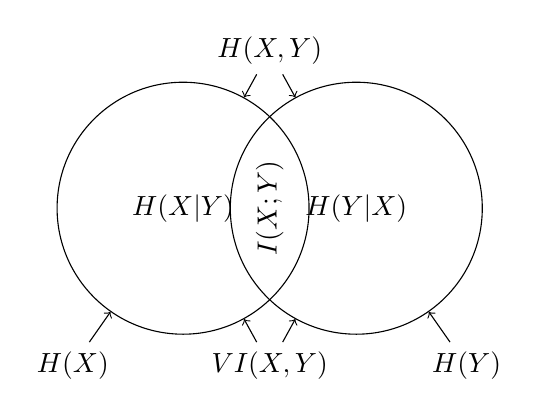
\begin{tikzpicture}
    \node[draw,circle,minimum size=3.2cm, inner sep=0cm] at (-1.1cm,0cm) (CL) {$H(X|Y)$};
    \node[draw,circle,minimum size=3.2cm, inner sep=0cm] at (1.1cm,0cm) (CR) {$H(Y|X)$};    
    \node[rotate=90] at (0cm,0cm) (IXY) {$I(X;Y)$};
    \node[] at (0cm,2cm) (HXY) {$H(X,Y)$};
    \node[] at (-2.5cm,-2cm) (HX) {$H(X)$};
    \node[] at (2.5cm,-2cm) (HY) {$H(Y)$};
    \node[] at (0cm,-2cm) (VI) {$VI(X,Y)$};
    \draw[->] (HX) -- (CL);
    \draw[->] (HY) -- (CR);
    \draw[->] (HXY) -- (CL);
    \draw[->] (HXY) -- (CR);
    \draw[->] (VI) -- (CL);
    \draw[->] (VI) -- (CR);
\end{tikzpicture}
\caption{Venn diagram representation of the important quantities used to treat the clustering comparison problem in terms of information theory.
The two circles are the entropies of variables $X$ and $Y$.
The mutual information $H(X;Y)$ is the intersection of the information in $X$ with the information in $Y$.
The Variation of information is equal to $VI(X;Y)=H(X|Y)+H(Y|X)=H(X)+H(Y)-2I(X;Y)$ because $I(X;Y)$ is counted twice.}
\label{fig:venn_diagram}
\end{figure}

\subsection{Confusion matrix}
It is also possible to quantify the confusion matrix $\mathbf{C}$ between the detected and planted modules.
Each element $C_{ij}$ is the number of nodes in the planted community $i$ that appear in the detected community $j$.
For each planted community one scores as true positives (TP) the nodes correctly identified as belonging to the ground-truth community, and as false positives (FP) the nodes wrongly assigned to a community; similarly false negatives (FN) are nodes wrongly classified in different communities and true negatives (TN) the nodes correctly classified as out of the community. Sensitivity, defined as $TP/(TP+FN)$, decreases with increasing number of False Negatives. Specificity instead is defined as $TN/(TN+FP)$ and decreases when many nodes are wrongly assigned in the same community. 

Accuracy (Acc) and Matthew Correlation Coefficient (MCC) are defined on the basis of the confusion matrix as:
\begin{align*}
\textrm{Acc}=\frac{(TP+TN)}{TP+FP+TN+FN} \, \textrm{MCC}=\frac{(TP\times TN-FP\times FN)}{\sqrt{(TP+FP)(TP+FN)(TN+FP)(TN+FN)}}
\end{align*}
where TP, TN, FP, FN are the number of true positives, true negatives, false positives and false negatives identified in the detected partition with respect to the planted partition.
Accuracy takes into account the proportion of correctly classified samples and can present relatively high values even in the case of poorly performing detection methods when the classes have very different size.
The Matthew Correlation Coefficient  takes into account true and false positives and negatives. It's a balanced coefficient, to use especially when classes are very imbalanced.


%%%%%%%%%%%%%%%%%%%%%%%%%%%%%%%%%%%%%%%%%%%%%%%%%%%%%%%%%%%%%
%%%%%%%%%%%%%%%%%%% PERCOLATION ANALYSIS %%%%%%%%%%%%%%%%%%%%
%%%%%%%%%%%%%%%%%%%%%%%%%%%%%%%%%%%%%%%%%%%%%%%%%%%%%%%%%%%%%
\section{Thresholding and percolation analysis}
\label{sec:percolation_analysis}
In weighted networks, sparsification procedures are often applied to remove the weakest edges, which are the most affected by experimental noise, and to reduce the density of the graph, thus making it theoretically and computationally more tractable.
Indeed, weak links may contain significant structural information~\cite{thomas2011}, and procedures to identify the optimal trade-off are the subject of active investigations~\cite{zahoranszky-kohalmi2016a}.
After sparsification, the network can be binarized, by setting all edge weights to unity.
Whether this procedure may help obtaining a better view on the underlying structure of networks, is an hot debate in the literature~\cite{rubinov2010,thomas2011}.

Ideally the obtained network should retain structural relations and ignore spurious links, but how is it possible to determine a proper value of threshold?
No well-accepted method to choose the best threshold has been adopted pragmatically in the brain networks literature and different scholars motivated their choice by different needs~\cite{gallos2012,lee2011,scheinost2012}.

Percolation analysis, a method originally grounded in statistical physics, was suggested by Gallos~\cite{gallos2012} to identify the optimal sparsification threshold for community detection in brain connectivity networks.
Percolation is a model to describe phase transitions of connected subgraphs in random networks~\cite{callaway2000,goerdt2001}.
In the ER random graph, the size of the largest connected component shows a sharp transition at some threshold value~\cite{callaway2000}.
Contrarily, brain networks exhibit multiple percolation thresholds, revealing a hierarchy of clusters as shown in Figure~\ref{fig:percolation_analysis_intro}.
The jumps corresponding to percolation transitions are indicative of non trivial correlations that constitute well defined modules of brain activity.
Hence, the multiple percolation thresholds are representative of a set of weak ties that guarantee appropriate communication (in terms of information transfer) between functionally specialized modules.
Following these observations, the definition of the optimal threshold is the one just above the fragmentation of the largest connected component.
This choice maximizes the information extracted by subsequent applications of community detection algorithms, and has been applied and validated in human~\cite{gallos2012} and animal~\cite{bardella2016a} studies.
\begin{figure}[htb!]
\centering
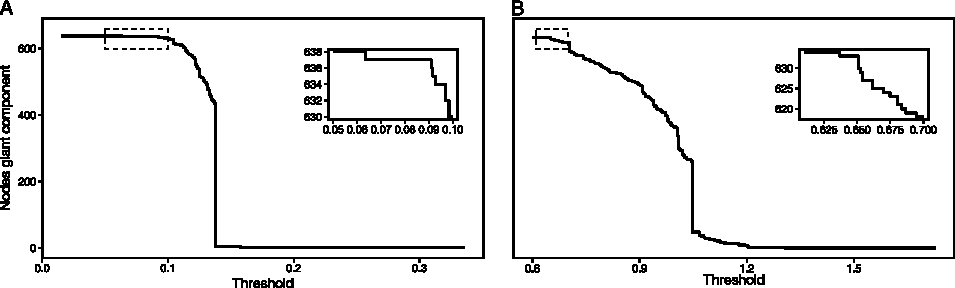
\includegraphics[width=1\linewidth]{images/percolation_analysis_side_by_side.pdf}
\caption{Percolation analysis for two brain networks available from the BrainConnectivityToolbox~\cite{rubinov2010}, available at~\url{https://sites.google.com/site/bctnet/}. (A) is a coactivation network, (B) a resting state network, both with 638 nodes and 18625 edges. The number of nodes in the giant component has a step-wise behaviour with respect to the threshold.}
\label{fig:percolation_analysis_intro}
\end{figure}

The most common choice when comparing networks from different groups, is to adopt a fixed threshold that keeps the same number of edges in the two groups.
This does not take into account the particularities of the analyzed group and datasets.
It is indeed important to stress that the distribution of the weights as well as the density or connectivity of the population are not exploited when using fixed thresholds and the final result does not mirror these information.
To this end, it has been demonstrated, especially in patients groups such as in schizophrenia, that the brain presents weaker functional connectivity than in healthy control persons~\cite{alexander-bloch2010}.

For this reason, percolation analysis should enable data-driven determination of the optimal sparsification threshold that preserves network structure and connectedness while removing potentially spurious correlations.




% The Matlab function that I used to determine the level of threshold is available on \texttt{CommunityAlg} Matlab toolbox at \url{github.com/carlonicolini/communityalg}.
% Functional connectivity networks are typically obtained as similarity matrices of physiological time signals over different brain areas.
% The process of converting similarity matrices into graphs, described in the previous chapters is not obvious.
% In most of the works, a threshold is chosen such that all the edge weights greater than a given value are kept, while other links, indicative of correlations due to possibly noisy components are discarded.

% Sparsification procedures are often applied to remove the weakest edges, which are the most affected by experimental noise, and to reduce the density of the graph, thus making it theoretically and computationally more tractable.
% Indeed, weak links may contain significant structural information~\cite{thomas2011}, and procedures to identify the optimal trade-off are the subject of active investigations~\cite{zahoranszky-kohalmi2016a}.

% As the final network density is of fundamental importance when performing community detection, the clustering outcome depends heavily on it.
% Hence, a completely data-driven thresholding procedure is needed, that helps in transforming a similarity matrix into a network.


\chapter{Modular organization of brain connectivity: the resolution limit}
\label{chap:modularorganization}
\vspace{2em}
%%%%%%%%%%%%%%%%%%%%%%%%%%%%%%%%%%%%%%%%%%%%%%%%%%%%%%%%%%%%%%%%%%%%%
%%%%%%%%%%%%%%%%%%%%%%%% COMMUNITY DETECTION %%%%%%%%%%%%%%%%%%%%%%%%
%\section{Community structure in the brain}
\section{Modularity of brain networks}
A systematic analysis of the structure of neural systems in different organisms points out that modularity is a factor that shapes neural networks from the small nematode worm \emph{Caenorhabditis Elegans} to the most complex human brain~\cite{meunier2010,towlson2013,park2013}. 
Topological network analyses suggest indeed that modular and hierarchical structural networks are particularly well-suited for the functional integration of locally specialized neural operations that underlie cognition~\cite{sporns2004,sporns2004a,bullmore2012,meunier2010,bressler2010}.
In this respect, brain function or cognition can be described as global integration of local integrators~\cite{park2013}.

Among the many advantages of a modular organization of the brain, three are of greatest importance and strictly intertwined: adaptability, robustness and wiring cost economy.
Firstly, from an evolutionary perspective, a modular architecture is highly adaptable to an ever changing environment and variable loads of cognitive demands.
From generation to generation, modules that were already well-fit to the environmental conditions were selected and passed, while others were only slightly rewired through the natural selection mechanisms. This pressure, together with the imperative of a reduced wiring cost have crucial to select an architecture that converged to a construction of tightly connected sub-networks loosely connected to each others~\cite{clune2013}.
Computational studies have shown that a modular organization emerges spontaneously in complex brain networks, promoting flexibility to an ever-changing outside environment~\cite{kashtan2005,kashtan2007} and maximizing bidirectional information exchange between neural populations~\cite{yamaguti2015}.

A second benefit of modularity is robustness as it facilitates evolvability and robust traits like the multiscale modular architecture are often selected by evolution~\cite{kitano2004,betzel2016}.
Indeed, keeping a system compartmentalized can limit the influence of external sources of perturbation, thus bounding the interdependence of biological processes going on in each unit~\cite{kirschner1998}, and promoting greater resilience in the context of continuous genetic and developmental changes.
In addition, swapping and rewiring maladaptive modules is less demanding that restructuring the whole system.
A general problem in the acquisition of new skills is the phenomenon of catastrophic forgetting, by which newly acquired skills come at the expense of others~\cite{french1999}.
In the case of neural networks it has been shown that a modular organization helps to avoid catastrophic forgetting of newly learned skills, whereby new skills are learned by slightly rewiring existing modules, rather than changing the overall organization~\cite{ellefsen2015}.
Local disruptive modification may only affect one module, whereas the others are preserved from the insult~\cite{stam2014}.
In case of externally or internally generated fluctuations, a modular architecture prevents functional disruption of the network leading to the possible death of the organism.

Thirdly, the spatial and metabolic constraints of neuronal wiring are factors that deeply shaped the brain architecture~\cite{bullmore2012,stam2012}. Computational and empirical studies converged on the result that a multiscale organization of modules inside modules is the one that satisfies the constraints imposed by minimization of energetic cost and spatial embedding~\cite{pan2007,bullmore2012,doucet2011,betzel2017,kaiser2006}.
Here, wiring cost must not only be intended as the physical volume of axons and synapses but also be considered in terms of energetic demand for signal transmission, additional processing cost for noise correction over long distance signalling and sustenance of the necessary neuroglia that supports neuronal activities~\cite{bullmore2012}. In terms of wiring cost reduction, modular networks emerge naturally when minimizing the average path length and the total number of links, while maximizing robustness against perturbations in node activity.
By way of example, in the field of robotics, spontaneous structural modularity of neural networks controllers emerge from evolutionary optimization when successful robot behaviour is encoded as fitness function~\cite{bongard2011}.

\bigbreak

Application of resting state fMRI has allowed the identification of various modules in human functional connectivity.
These spatially distinct modes that demonstrate synchronous BOLD fluctuations, consist in strongly correlated, anatomically separated, possibly remote regions of the brain~\cite{biswal1995,raichle2001,fox2005,biswal2012}.
Various methods exist for analyzing resting-state data, including seed-based approaches~\cite{biswal1995,raichle2001}, independent component analysis~\cite{beckmann2005,damoiseaux2006} and graph-based methods~\cite{stam2007,bullmore2009}. They have generally shown that the human brain is functionally organized in a number of interconnected regions with boundaries that reflect specific aspects of cognitive and behavioural aspects~\cite{tomasi2012,alnaes2015,crossley2013a}.
The first analysis method ever used was the seed-based approach~\cite{biswal1995}, which has been applied in numerous studies~\cite{raichle2001}.
This technique is based on the correlation of voxels within selected regions of interest (ROIs), with the average BOLD signal from all other voxels in the brain.
An accurate thresholding is then needed to identify voxels that are significantly correlated with the region of interest.

Another widely used approach is the decomposition of the endogenous BOLD fluctuations by means of Independent Components Analysis, a technique that aims at maximizing statistical independence between time courses of single voxels and that can identify separate spatial modes~\cite{damoiseaux2006,beckmann2005,calhoun2013}.
Yet, ICA with its variants still relies on user experience to discern important components from noise~\cite{lee2013} and despite some notable attempts to identify noise~\cite{thomas2002,tohka2008}, like seed-based approaches, does not yield any information on the hierarchy of modes, nor on their relation.
Moreover, largely overlapping results can be obtained by ICA and seed-based approaches~\cite{rosazza2012}.

The evidence of modules in human functional networks is based on their robustness and consistency within a variety of MRI protocols, different analysis methods, and MRI scanners. 
Differently from structural networks, since functional networks do not measure physical relations with associated metabolic or material cost, they may feature long-distance connections~\cite{dehaene1998,varela2001} and ever changing patterns.
The majority of analysis techniques are concordant in identifying a set of robust functionally linked regions, or \emph{modules} in resting state networks.
These modules, roughly highlighted with coloured ellipses in Figure~\ref{fig:vandenheuvelnetworks} span the primary somatosensory network, the primary visual and extra-striate network, a network consisting of bilateral temporal/insular areas and anterior cingulate cortex regions, left and right lateralized networks consisting of superior parietal and superior frontal regions (often reported as one single network) and the so-called default-mode network spanning precuneus, medial frontal, inferior parietal cortical regions and medial temporal lobe.
\begin{figure}[!htb]
\centering
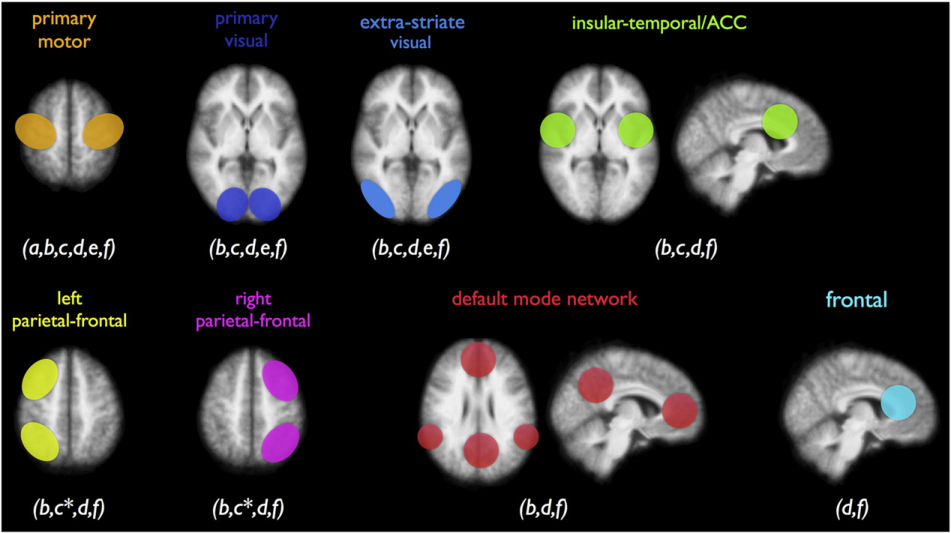
\includegraphics[width=1.0\textwidth]{images/vandenheuvel_networks.pdf}
\caption{Functional modules of the resting state brain, averaged over different studies and protocols, and visualized roughly on a brain template to indicate their anatomical position. Figure taken from~\cite{vandenheuvel2010}.}
\label{fig:vandenheuvelnetworks}
\end{figure}
The Default Mode Network, or DMN, firstly identified by Raichle~\cite{raichle2001} with positron emission tomography and then confirmed by Greicius et al. using fMRI~\cite{greicius2003} is one of the most consistent networks among a variety of studies. It comprises a group of spatially remote brain regions that show higher levels of correlation when the brain is not involved in any particular cognitive or behavioural task.
For this reason, it is hypothesized that there are two opposing concurrent large scale modes, one including the DMN, indicated as ``task-negative'' or ``intrinsic'' system, and the other comprising regions involved in attentional and task evoked activities, dubbed ``task-positive'' or ``extrinsic'' system~\cite{power2011,fox2002,golland2008}.
The Default Mode Network or DMN (Figure~\ref{fig:vandenheuvelnetworks}) is thought to be connected to high-level cognitive functions, given its specific traits of structural links to associative brain regions and that the DMN may support internal mental processing like mind-wandering, abstract thinking and planning of events in the future~\cite{gusnard2001,buckner2008}.
Additionally, evidence has pointed to disruptions in the DMN with people with Alzheimer's disease~\cite{buckner2008}, autism spectrum disorders~\cite{washington2014} and schizophrenia~\cite{garrity2007}.

Apart from the DMN and networks for the primary sensory areas, other networks have different roles, many of which are partly speculative.
Subcortical communities have also been identified with rs-fMRI: an appropriate ICA seeding, makes possible to observe functional modules located at the thalamus and hippocampus~\cite{lee2012}.
Modules in functional brain networks have been explained as the possible basis of a large variety of neural processes.
By way of example, certain functional processes, like colour vision, have been described as anatomically localized~\cite{zeki1998}, while others, like working memory, have been proposed to involve more globally integrated processing systems~\cite{dehaene1998,baddeley2003}.
Interestingly modules of functional brain networks are non-static as recent studies found that they tend to become less and less modular with ageing~\cite{meunier2009a,song2014}.
In all respects, the experimental indication of the modular organization is a powerful and robust marker against which to measure the health of the brain. 
Thus, modularity is not only a biologically plausible feature but it is very likely necessary to maintain the rich repertoire of cognitive tasks that our brain engages in every day of our life.

Modeling of resting state networks by means of graph-theory provides a compelling alternative to seed-based and ICA approaches.
Within this framework ROI are nodes of a network, connected by edges of weight proportional to the strength of correlation between ROIs.
Graph-theory offers a wide amount of measures to characterize functional connectivity networks and in particular a wealth of methods to identify communities, subsets of nodes which are more strongly correlated between each other, than with external nodes~\cite{bullmore2009,stam2014,sporns2016}.

Interestingly, the size distribution of the functional modules has never been analyzed in details, especially when graph-theoretical methods were applied.
This is the case of one of the most fortunate and widely adopted method to identify modules in functional networks, Newman's Modularity~\cite{newman2006}.
Despite its popularity and merits, Newman's approach presents some important limitations.
Already at an early stage, Modularity-based methods were shown to suffer from a resolution limit, as they fail to identify modules that are smaller than a scale that depends on the size of the overall network~\cite{fortunato2007}.
As a consequence, even unambiguously defined modules, like complete sub-graphs or cliques, may be unduly merged into larger communities when they are too small compared to the size of the network.
Subsequent work by various groups has shown that the resolution limit is quite pervasive~\cite{lancichinetti2009,traag2011,squartini2015,lancichinetti2011,kawamoto2015}, and affects, to a different extent, many other methods, including Reichardt and Bornholdt’s~\cite{reichardt2006}, Arenas and Gomez'~\cite{arenas2008}, Ronhovde and Nussinov's~\cite{ronhovde2009}, Rosvall and Bergstrom's (\emph{Infomap})~\cite{rosvall2008,kawamoto2015} and others.

Fixes have been proposed to circumvent the resolution limit, including the introduction of a tunable parameter that enables analysis of the network at an adjustable resolution level~\cite{reichardt2006,ronhovde2010,yeo2011}. However, this requires prior knowledge of the expected size of the communities for the tuning of the resolution parameter. Moreover, it has been shown that an  adjustable resolution parameter may reduce the tendency to merge small clusters, but only at the cost of unduly splitting large clusters~\cite{lancichinetti2011}. Adjustment of the resolution parameter is an attempt to balance these two biases, but multiresolution methods fail to recover community structures comprising heterogeneous distributions of cluster sizes~\cite{lancichinetti2011}. 
However, real-world networks are characterized by the coexistence of clusters of very different sizes, and no single parameter can adapt to the variety of network topologies observed in nature.
Hence, the resolution limit may represent a critical shortcoming for the study of brain networks and is likely to have affected many of the studies reported in the literature.

In the following sections I'm going to illustrate the current graph-theoretical approaches for community detection in networks and to discuss the theory of community detection, highlighting the practical problems of Modularity maximization.



		% A number of other resting-state networks has been identified

		%  Studies have hypothesized that there are
		% 2 large opposing systems in the brain, one including the DMN and
		% the other composed of attentional or task-based systems, such as
		% somatosensory, visual, or attention RSNs. Terms used to refer to
		% these systems include “task-positive” and “task-negative”4,12,13
		% and “intrinsic” and “extrinsic.”14,15
		% Several other RSNs have been identified. The somatosensory
		% network, studied first by Biswal et al,1 includes primary and
		% higher order motor and sensory areas (Fig 1B). The visual network
		% is highly consistent across various studies and spans much of
		% the occipital cortex (Fig 1C).2-6An auditory network consisting of


		% Another popular approach is ICA,2,10 a mathematical technique
		% that maximizes statistical independence among its components.
		% For RS-fMRI data, ICA can be used to spatially identify distinct
		% RSNs. Compared with seed-based methods, ICA has the advantage
		% of requiring few a priori assumptions but does compel the
		% user to manually select the important components and distinguish
		% noise from physiologic signals. Some studies have aimed to
		% automate this process and use ICA as a method for identifying
		% noise within the BOLD signal.33-36 Despite the differences in the 2
		% approaches, Rosazza et al37 showed that the results of seed-based
		% analysis and ICA are significantly similar in a group of healthy
		% subjects.
		% Graph methods provide a distinct alternative to seed-based
		% analyses and ICA.4,38-44 This approach views RSNs as a collection
		% of nodes connected by edges. With RS-fMRI data, ROIs can be
		% represented as nodes, and correlation between the ROIs, as the
		% connectivity of the edges. Connectional characteristics of the
		% graph can then be computed.44 Examples of measures of interest
		% include the average path length, a measure of global connectedness,
		% which is the average length of the shortest connection between
		% all pairs of nodes.44 Another measure of interest is the clustering
		% coefficient, which is related to the connectedness of
		% neighboring nodes and reflects the presence of smaller subgraphs.44
		% Using these techniques, several studies have demonstrated
		% that the brain exhibits a small world topology. Small world
		% topology, which was first described in social networks, allows each
		% node to have a relatively low number of connections while still
		% being connected to all other nodes with a short distance. This is
		% achieved through the existence of hubs, which are critical nodes
		% with large numbers of connections, that allow high levels of local
		% connectivity.39,45 Small world networks have high clustering coefficients
		% implying high levels of local connections (ie, cliques or
		% groups) and an overall short distance between any 2 nodes, or a
		% small average path length.40-42


%%%%%%%%%

% % Unfortunately, until recently most of the studies in animal models were based on anatomical connectivity measured by means of post-mortem inspections.
% % While in the past, histological staining was the most adopted methodology to inspect the wiring of white matter in the animal brain, the last few decades have seen the rising of fluorescence based tract-tracing, that evolved to a level where single axons can be traced with unprecedented precision~\cite{oh2014}.
% % Not only methods to investigate the structural connectivity have greatly evolved, but also new cellular resolution recording systems, like light-sheet microscopy~\cite{ahrens2013}, real time in-vivo two-photon cortical imaging~\cite{dombeck2010,leinweber2014} and spike time series recordings on multielectrode arrays~\cite{shimono2015}.
% % All these techniques take part in the quest to shed light on the relation between functional networks and their underlying anatomical substrate.

% After the discovery of low frequency fluctuations of the BOLD signal of the brain at rest~\cite{biswal1995}, 
% In humans, non-invasive studies of the brain community structure largely reflect the analytical methodologies adopted in animals.
% In both contexts, functional connectivity is suggested to describe the relationship between neuronal activity patterns of anatomically separated regions that reflect the level of information exchange between them.
% The decomposition of the endogenous fluctuations of the BOLD signal at rest by means of independent components analysis (ICA), showed a repertoire of \emph{spatial modes}, clusters of brain regions whose neural activity oscillates synchronously. These patterns of spontaneous coupled oscillations are strongly correlated between anatomically separated, possibly remote regions of the brain~\cite{biswal1995,raichle2001,fox2005,biswal2012}. Additionally, these patterns of functional connections that derive from a modular architecture of the brain, are themselves modular. A submodule (or subnetwork), often called community in graph theory, comprises synchronously active voxels. The enduring and stable synchrony within those voxels is thought to reflect local integration processes



% The evidence of modules in functional brain networks has been explained as the possible basis of a large variety of processes. By way of example, certain functional processes, like color vision, have been described as anatomically localized~\cite{zeki1998}, while others, like working memory, have been proposed to involve more globally integrated processing systems~\cite{dehaene1998,baddeley2003}.
% Interestingly modules of functional brain networks are non-static as recent studies found that they tend to become less and less modular with aging~\cite{meunier2009a,song2014}. 
% In all respects, the experimental evidence of the modular organization is a powerful and robust marker against which to measure the health of the brain. 
% Thus, modularity is not only a biologically plausible feature but it is probably necessary to maintain the rich repertoire of cognitive tasks that our brain engages in every day of our life.

% Despite the biological evidence of modularity in brain networks, the number of modules returned by clustering methods is often chosen in advance, based on the experience of the researcher, even if some complex approaches are available~\cite{still2004}. 

%%%%%%%%%%%%%%%%%%%%%%%%%%%%%%%%%%%%%%%%%%%%%%%%%%%%%%%
%%%%%%%%%%%%%%%%%%%%%%%%%%%%%%%%%%%%%%%%%%%%%%%%%%%%%%%
%%%%%%%%%%%%%%%%%%%%%%%%%%%%%%%%%%%%%%%%%%%%%%%%%%%%%%%

\section{Community detection in networks}
\label{sec:communitydetectioninnetworks}
The process of grouping nodes in a graph to establish their common behavioral properties is a popular technique that goes under the name of \emph{community detection}.
Following the initial work by Hilgetag~\cite{hilgetag2000a} dubbed OSA (Optimal Set Analysis), several graph theoretical methods have been deployed to investigate the modular structure of structural and functional brain networks~\cite{meunier2009,meunier2010,power2011,stam2007,stam2014}.
Typically, these methods rely on the optimization of a fitness function that measures the quality of a network partition against that of an ensemble of randomized networks with similar statistical properties, called the ``null model''.
Optimization of the fitness function of choice is often computationally demanding and scales steeply with increasing network size.
Hence, heuristics are needed to calculate nearly optimal partitions of large networks, like those derived from neuroimaging data, within reasonable computation time~\cite{blondel2008,rosvall2008,raghavan2007}.
As the definition of community is not unambiguously stated, it is therefore, important to have a quantitative way to evaluate the goodness of such clusterings.

A global criterion for the definition of communities in networks can be thought in terms of a fitness function defined over the clustering.
A \emph{quality function} is a function $\mathcal{Q}$ that given a clustering of a graph $\zeta$ returns a scalar number. Usually one identifies ``good'' clusterings with high scores of the quality function and ``bad'' clusterings with low scores. In this sense, it is possible to rank partitions from bad to good, although is important to stress that the definition of good or bad clusterings is an \emph{ill-posed problem} as every quality function puts emphasis on some features and perhaps not on others. 
Here and in the following sections, it must be stressed that the concept of quality function and community detection methods are separate as the first is a way to assess the goodness of a partition while the second relies on the definition of a quality function to design efficient algorithms and heuristics to find such good partitions.

One of the most important properties of a quality function is additivity, i.e. its expression as a sum of terms each pertaining to a single community.
For a generic function of a cluster, or subgraph, $f(\zeta_i)$, an additive quality function specify the goodness of a clustering as the sum of $f$ over the distinct communities as follows:
\begin{equation}\label{eq:additive_quality}
\mathcal{Q} = \sum \limits_{\zeta_c \in \zeta} f(\zeta_c).
\end{equation}
The majority of quality functions are additive, even if this requirement is not strictly required.
In the next section, we explore the properties of some of the most important additive quality functions that emerged from the literature in this decade.

\subsection{Spin glass based quality functions}
The simplest formulation of a quality function is one that puts emphasis on intracluster edges and penalizes intercluster edges.
In this terms, local optima of the quality function should correspond to partitions where the communities emerge as dense areas in the network loosely connected among them.
A framework grounded in statistical mechanics for the definition of suitable quality functions for community detection that meet these requirements has been introduced by Reichardt and Bornholdt (RB)~\cite{reichardt2006}.

In the RB model the problem of community detection is cast in terms of finding the \emph{ground state} of a spin glass, a model describing the behavior of large sets of interacting microscopic magnets.
Actually, the properties of spin glass models are subject of intensive research in the last decades as their applications range from condensed matter and nuclear physics to neural networks. Here we present only their salient application to community detection and refer the reader for the details of the model to more specialized books~\cite{mezard1990}.

A spin glass model is based on the definition of an Hamiltonian, a multi-variable scalar function that describes the total energy of the physical system with the configuration of its internal components.
In our case, the internal components of the system are the nodes. The configuration of the system is then expressed by the community affiliation vector $\boldsymbol\sigma$, meaning that node $i$ stays in the community $\sigma_i$.
The Hamiltonian used by Reichardt and Bornholdt (RB) includes four different contributions. The first two contributions act at intracluster level, positively weighing intracluster edges and negatively weighing intracluster non-edges with coefficients $a_{ij}$ and $b_{ij}$ respectively. The third and fourth contributions work on intercluster edges and non-edges, weighing them with factors $c_{ij}$ and $d_{ij}$. The general form of the RB model is then expressed by the following Hamiltonian:
\begin{align}\label{eq:hamiltonianspinglass}
\mathcal{H}^{\textrm{RB}}(\boldsymbol \sigma) = - \sum_{(i,j)\in V^2} & \left[ a_{ij} A_{ij} - b_{ij}(1-A_{ij}) \right] \delta(\sigma_i,\sigma_j) + \nonumber \\ &  \left[ (c_{ij} A_{ij} - d_{ij}(1-A_{ij}) \right] (1-\delta(\sigma_i,\sigma_j)),
\end{align}
with the convention that lowest energy states correspond to best community assignments.
Rearranging Eq.\ref{eq:hamiltonianspinglass} and collecting the terms independent of the partition into a constant $H_0$, one then gets a simpler expression for $\mathcal{H}^{\textrm{RB}}(\sigma)$:
\begin{equation}\label{eq:rbspinglass}
\mathcal{H}^{\textrm{RB}}(\boldsymbol \sigma) = -H_0 - \sum \limits_{(i,j)\in V^2} \left[ \alpha_{ij} A_{ij} - \beta_{ij} \right] \delta(\sigma_i,\sigma_j),
\end{equation}
where the two parameters $\alpha_{ij}=a_{ij}+b_{ij}+c_{ij}+d_{ij}$ and $\beta_{ij}=b_{ij}+d_{ij}$ depend on the \emph{null model}, i.e. the probability that an edge exists between $i$ and $j$ after random edge rewiring. Hence, a null model provides a mean to compare a specific set of features of a graph, with its randomized version that should specifically lack those features.

% It's possible to express any additive quality function in the form of Eq.~\ref{eq:rbspinglass} as an additive quality function by setting $\alpha_{ij}=1$, $H_0=0$ , as the sum is only over intracluster edges.
Setting $\alpha_{ij}=1$, $H_0=0$ and moving the summation indexes over the communities rather than over the pairs of nodes, one can express the resulting Hamiltonian, as an additive quality function expressed here as $\mathcal{H}^{\textrm{RB}}_{\textrm{reduced}}(\sigma)$, that reads:
\begin{equation}\label{eq:rbspinglass2}
\mathcal{H}^{\textrm{RB}}_{\textrm{reduced}}(\sigma) = -\sum_{(i,j) \in V^2} \left[ A_{ij} - \beta_{ij} \right] \delta(\sigma_i,\sigma_j) = - \sum \limits_{c}^C \left[ m_c - \left< m_c \right> \right].
\end{equation}
where $m_c=\sum_{ij}A_{ij}\delta(\sigma_i,c)\delta(c,\sigma_j)$ represents the number of links inside community labeled by $c$ and $\left <m_c \right >=\sum_{ij}\beta_{ij}\delta(\sigma_i,c)\delta(c,\sigma_j)$ is the expected number of links in community $c$ as prescribed by the null model $\beta_{ij}$\footnote{Here and for the rest of the work, we set $P_{ij}:=\beta_{ij}$ for agreement with more conventional notation of null models}. 
Among the additive quality functions that show up in the form of~\ref{eq:rbspinglass2}, the most important and popular is \emph{Newman-Girvan's Modularity}.

\subsection{Newman-Girvan Modularity}\label{sec:newman_modularity}
Newman-Girvan Modularity (or simply Modularity)~\cite{newman2006}, denoted here and for the rest of the work by $Q^N$, is based on the idea that a network obtained by randomly reshuffling the original graph edges while keeping the same degrees sequence, should not display any community structure. 
An important consequence of such randomization is that any stub in this null model, dubbed ``configuration model'' is equally likely to be connected to any other~\cite{newman2010book}. Thus, in absence of correlations, the probability that two nodes are connected is expressed by:
\begin{equation}\label{eq:configuration_model}
P_{ij} = \frac{k_i k_j}{2m},
\end{equation}
where $k_i$ and $k_j$ are the degrees of node $i$ and $j$. The ``configuration model''  is of great importance in network science as it assigns a higher probability of linking to nodes with high degrees, a feature that is compatible with most real world networks~\cite{newman2010book}.
The motivations of the configuration model are addressed in details in section~\ref{sec:configuration_model}.

In terms of a spin glass model, Modularity measures the deviation from the observed intracluster density with respect to the expected intracluster density specified by the configuration model. Modularity is described in the form of~\ref{eq:rbspinglass2} but normalized by the number of edges in the graph, taking the form described in Eq.~\ref{eq:newmanmodularityspinglass}.
\begin{equation}\label{eq:newmanmodularityspinglass}
Q^N =  \frac{1}{2m} \sum_{ (i,j) \in V^2} \left[ A_{ij} - \frac{k_i k_j}{2m} \right] \delta(\sigma_i,\sigma_j),
\end{equation}
whereby optimal partitions have high values of $Q^N$. As shown in Eq.~\ref{eq:rbspinglass2}, Modularity can be expressed as sum over communities of the difference of two terms:
\begin{equation}\label{eq:newmanmodularity}
Q^N = \sum_{c}^{|C|} \left[ \frac{m_c}{m} - \left( \frac{K_{\textrm{int}}(\mathcal{G}_c)}{2m} \right)^2 \right].
\end{equation}
Modularity takes values in the range $[-0.5,1]$, then a good partition should have $Q^N$ values close to unity, identifying groups with much more internal connections than expected at random. In contrast, a bad partition with $Q^N$ close to zero should identify groups with no more internal connections than we expect at random.
In the next sections we will challenge this idea and show that this observation has led to false statements, as a general phenomenon, dubbed \emph{resolution limit}, heavily affects any quality function based on comparison with global null models.
Specifically, in the case of Newman's Modularity, the resolution limit hampers its ability to detect modules smaller than a scale determined by the size of the graph.

\subsection{The configuration model}\label{sec:configuration_model}
A central property of the configuration model is the probability $P_{ij}$ of the occurrence of an edge between two specified vertices $i$ and $j$.
In absence of correlations, as prescribed by the random reshuffling imposed by the configuration model, the probability that a stub emerging from vertex $i$ is connected by an edge to any of the stubs of vertex $j$ is $k_j/(2m-1)$ as there are $2m-1$ stubs in total.
Therefore the total probability that vertex $i$ and vertex $j$ are connected by an edge is the product of the stub probability times the number of stubs from vertex $i$, namely 
\begin{equation}\label{eq:configuration_model_probability}
P_{ij} = \frac{k_i k_j}{2m-1} \approx \frac{k_i k_j}{2m}.
\end{equation}
Although the configuration model is most frequently applied to \emph{simple graphs} (Figure~\ref{fig:simple_unweighted_graph}), the configuration model implies that the randomization is carried over the space of \emph{loopy multigraphs} (Figure~\ref{fig:loopy_multigraph}).
The rewiring probability considers indeed that the stubs of nodes can be reconnected both to the same source vertex (self-loops) or added to already existing edges (multi-edges).
Consider for example the set of matchings on six stubs that form a triangle graph as illustrated in Figure~\ref{fig:configuration_model_stubs}. The configuration model chooses each distinct edge stubs labeling with equal probability. However, not only the first eight distinct reshuffled labelings are possible under configuration model (Fig.\ref{fig:reshuffle_simple_graphs}) but many other distinct matchings producing non-simple networks as shown in Figure~\ref{fig:reshuffle_loopy_multigraphs}.

In practice, though, the fraction of edges involved in either self-loops or multi-edges is vanishingly small in the large $n$ limit, and thus we may generally ignore them without much impact. 
Hence, the estimate of the probability of rewiring in Eq.~\ref{eq:configuration_model_probability} is only valid in large, sufficiently sparse graphs with a sufficiently bounded degree sequence.
Under these hypotheses the expected number of edges between two vertices in the space of simple graphs is asymptotically the same as the expectation in the space of stub-labeled loopy multigraphs, i.e. the one previously introduced for the definition of Modularity: $\mathbb{E}_s[a_{ij} |k] \approx k_i k_j /(2m)$, where the subscript $s$ denotes the space of simple graphs.

\begin{figure}[htb]\centering
\begin{subfigure}[t]{0.45\textwidth}\centering
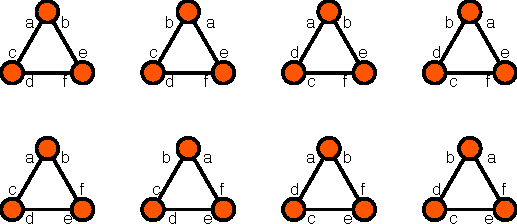
\includegraphics[height=2.4cm]{images/configuration_model_six_stubs.pdf}
\caption{}
\label{fig:reshuffle_simple_graphs}
\end{subfigure}
\begin{subfigure}[t]{0.45\textwidth}\centering
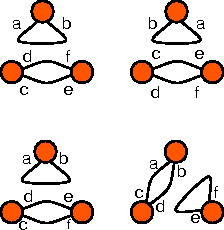
\includegraphics[height=2.4cm]{images/configuration_model_three_stubs.pdf}
\caption{}
\label{fig:reshuffle_loopy_multigraphs}
\end{subfigure}
\caption{Twelve of the ninety different possible rewirings of a triangle graph in the configuration model. In (a) only rewirings leading to simple graphs are considered. In (b) just four rewirings leading to loopy-multigraphs are shown.}
\label{fig:configuration_model_stubs}
\end{figure}
An approach that allows to get the right configuration model depending on the class of graph under exam, relies on the computational simulation of the correct rewiring probability by means of Markov Chain Monte Carlo algorithms, as proposed in~\cite{fosdick2016}.
In the remaining paragraphs, although flawed, we'll use the classic configuration model from Eq.~\ref{eq:configuration_model_probability} to be adherent to most of the brain networks literature, justified also by the vanishing effects of self-loops in large sparse networks. Nonetheless, we will illustrate many of the problems that the noncritical use of Modularity with this null model has introduced.

%%%%%%%%%%%%%%%%%%%%%%%%%%%%%%%%%%%%%%%%%%%%%%%%%%%%%%%%%%%%%%%%%%
%%%%%%%%%%%%%%% OTHER NULL MODELS FOR MODULARITY  %%%%%%%%%%%%%%%%
%%%%%%%%%%%%%%%%%%%%%%%%%%%%%%%%%%%%%%%%%%%%%%%%%%%%%%%%%%%%%%%%%%
\subsection{Other null models for Modularity}
Modularity identifies communities as the subset of nodes whose internal fraction of edges deviates from the null configuration model on the same subset with the term $m_c/m > (K_c/2m)^2$.
Despite measuring deviation from a null model, Modularity does not take into account the statistical evidence associated with this deviation. For this reason, Modularity is not able to separate actual communities from those arising only from statistical fluctuations of the null model. Even worse, Modularity can find high-scoring partitions in fully random graphs~\cite{guimera2004} and in artificially built graphs with no community structure~\cite{kehagias2013}.

The configuration model is not the only possible null-model to use in spin-glass based quality functions. Different authors proposed several variants of Modularity~\cite{ronhovde2010,ronhovde2009,traag2011} with different null models.
The simplest variation of Modularity is the so-called ER Modularity~\cite{traag2015} that instead of the configuration model uses an Erd\H{o}s-Rényi random graph in which every edge appears with the same probability $p_{\textrm{ER}}$. The number of expected edges $\left< m_c \right>$ in a community of size $n_c$ is thus (in the space of simple graphs):
\begin{equation}
\left< m_c \right> = p_{\textrm{ER}}\binom{n_c}{2}.
\end{equation}
and plugging this null model into the RB model of Eq.~\ref{eq:rbspinglass2} we obtain the model:
\begin{equation}\label{eq:ermodularityrb}
\mathcal{H}^{ER} = -\sum \limits_c^C \left[\frac{m_c}{m}  - p_{\textrm{ER}}\binom{n_c}{2} \right].
\end{equation}
As the most similar ER graph of a given graph is the one that matches its density, the probability parameter $p_{\textrm{ER}}$ must be set equal to the original empirical graph density $\rho$. The so-called ER Modularity is derived by plugging the graph density into Eq.\ref{eq:ermodularityrb} and inverting its sign: 
\begin{equation}
Q^{ER} = \sum \limits_c^C \left[\frac{m_c}{m}  - \rho \binom{n_c}{2} \right].
\end{equation}
Under this model, a group of nodes forms a community if its internal density is greater than the graph density $\rho$, on average.
Interestingly, from a machine learning perspective, all spin glass models quantify the discrepancy between observed and expected intramodular fraction of edges by means of a linear loss function. Among all the loss function, the linear is not the only possible and loss functions that take into account the relative size of clusters are possible.


%%%%%%%%%%%%%%%%%%%%%%%%%%%%%%%%%%%%%%%%%%%%%%%%%%%%%
%%%%%%%%%%%%%%% RESOLUTION-LIMIT  %%%%%%%%%%%%%%%%%%%
%%%%%%%%%%%%%%%%%%%%%%%%%%%%%%%%%%%%%%%%%%%%%%%%%%%%%
\section{Resolution limit}\label{sec:resolutionlimit}
Modularity attracted a lot of attention over the years as it became the tool of election to inspect the community structure of networks.
On one side, the wide use of Modularity led many researchers to gain interest in complex networks, with applications in sociology~\cite{li2008tag}, bioinformatics~\cite{saracc2012topology} and ICT~\cite{java2007we,leskovec2007dynamics}, just to mention a few. On the other hand, it offered a fallacious view on the community detection problem.
Indeed, although simple in many sense, Modularity optimization was hiding a problem that heavily limits its use in real world networks.

In 2007, a seminal article by Fortunato and Barthelemy~\cite{fortunato2007} did a thorough analysis of Modularity.
Their work showed the inability of Modularity to correctly identify communities that are smaller than a certain scale, determined by the square root of the total number of edges. They dubbed this general phenomenon \emph{resolution limit}.
To illustrate what is meant by the resolution limit, here we follow the example of Fortunato and Barthelemy, with some obvious notational change.

Let us consider a toy network, $G=(V, E)$ that is composed of three subnetworks, as shown in~\ref{fig:figure_1_barthelemy}A.
The first subnetwork, a subgraph $G_0$ with $n_0$ nodes and $m_0$ edges is connected to two cliques, $G_1$ and $G_2$ by $m_{01}$ and $m_{02}$ links respectively.
The two cliques are also connected by a number of $m_{12}$ links as shown in Figure~\ref{fig:figure_1_barthelemy}.
While $G_1$ and $G_2$, are complete subgraphs and modules by construction, $G_0$ may consist of many communities.
Maximum Modularity partitions then, should identify $G_1$ and $G_2$ as communities, independently from $G_0$.
To be more specific, let the partition where the two cliques are separated be denoted by $A$, with Modularity value $Q_A$.
On the other hand, the partition where the two cliques are merged into a single community is denoted by $B$, with Modularity value $Q_B$.
To ease the calculations, we indicate the number of links $m_{12}$ as functions of $m_1$ and $m_2$, such that $m_{12}=a_{1}$, $m_1=a_2 m_2$, $m_{01}=b_1 m_1$ and $m_{02}=b_2 m_2$ with $a_1,a_2,b_1,b_2 \geq 0$.

As Modularity is a sum over the modules, and the module $G_0$ has the same Modularity $Q_0$ in both partitions, we are interested in studying the difference $\Delta Q = Q_{A} - Q_{B}$. After some simple algebraic manipulations it results:
\begin{equation} \label{eq:resolution_limit_delta}
\Delta Q = \frac{2 m a_1 m_1 - (a_1+b_1+2)(a_2+b_2+2)m_1 m_2}{2m^2}
\end{equation}
Specifically, we want to find the conditions whereby $\Delta Q > 0$, i.e. when the partition $A$ has a higher Modularity than partition $B$. This inequality is verified as long as
\begin{equation}
m_2 < \frac{2m a_1}{(a_1+b_1+2)(a_2+b_2+2)}.
\end{equation}
In the case where $a_1=a_2=0$, there are no links between $G_1$ and $G_2$ and the condition is satisfied. When the two subgraphs are connected ($m_{12} \neq 0$), it happens that at some values of $m_1$ and $m_2$ the partition where the two modules are merged is preferred, i.e. $\Delta Q <0$. This means that when maximizing $Q^N$ on a network, is possible to miss some important structures, if they are too small.
More specifically, if the two modules have the same size and one sets $a_1=a_2=b_1=b_2=1/m$, is easy to verify that Eq.~\ref{eq:resolution_limit_delta} is not satisfied if the number of links in the modules $m_c$, is lower than the square root of the total number of links in the network:
\begin{equation}
m_c < \sqrt{\frac{m}{2}}.
\end{equation}
To make this example more concrete we studied numerically a toy network where the three subgraphs take a precise form.
For the sake of illustration, we have defined $G_1$ and $G_2$ as two identical cliques of $5$ nodes connected to $G_0$ by a single edge ($m_{01}=m_{02}=1$) and to each other by $m_{12}$ edges.
The module $G_0$ was defined as a clique of variable size with a number of edges ranging from 45 to 2775. We then computed the numerical difference $\Delta Q$ and plotted it as a function of the number of edges $m_0$ in the $G_0$ clique.

\begin{figure}[htb!]
\centering
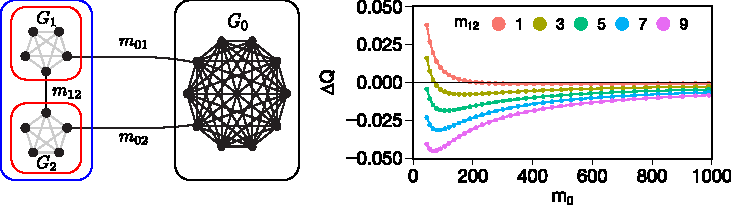
\includegraphics[width=1\textwidth]{images/barthelemy_modularity.pdf}
\caption{Analysis of the onset of the resolution limit for Modularity in a model graph (A) consisting of two cliques, $G_1$ and $G_2$, and a size-varying components $G_0$. The red line indicates the partition $A$, with $G_1$ and $G_2$ as different modules, and the blue line the partition $B$, with $G_1$ and $G_2$ merged into a single module. The graph (B) shows the difference in Modularity for increasing number of edges in $G_0$.}
\label{fig:figure_1_barthelemy}
\end{figure}

The onset of the resolution limit occurs when $\Delta Q$ changes sign and becomes negative for increasing values of $m_0$.
For $m_{12}=1$, i.e. when the two cliques $G_1$ ad $G_2$ were connected by only one edge (red curve), $Q$ showed this sign inversion for $m_0 \approx 200$ (Figure \ref{fig:figure_1_barthelemy}B).
With an increasing number of intercluster edges $m_{12}$, the resolution limit appeared for smaller and smaller values of $m_0$, eventually leading to $\Delta Q$ values that were always negative, i.e. the two cliques $G_1$ and $G_2$ were always merged by Modularity optimization.
An even more striking example of how the resolution limit affects Modularity is when looking at the optimal partition of a synthetic lattice graph, known as ``ring of cliques'', a network made out of identical cliques, connected in a ring-like structure by single links, as shown in Figure~\ref{fig:traag_ring_of_cliques}. In this toy network, the intracommunity density is the highest possible, while the intercommunity density is the lowest as to keep the network connected.
\begin{figure}[htb!]
\centering
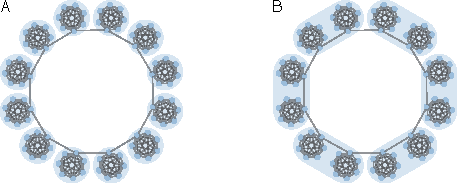
\includegraphics[width=1\textwidth]{images/traag_ring_of_cliques.pdf}
\caption{The ring of cliques toy model. The left panel (A) shows the ground truth partition with maximal intracluster density and minimal intercluster density. The right panel (B) shows the maximum Modularity partition, whereby cliques are coalesced in pairs.}
\label{fig:traag_ring_of_cliques}
\end{figure}
If the number of cliques is large enough (they are more than $\sqrt{m}$), Modularity optimization leads to a partition where the cliques are combined into groups of two or more. This phenomenon can be observed already when considering a ring of 30 cliques made of 5 nodes, when the optimal Modularity partition combines cliques in pairs.
Yet, extending the number of cliques, Modularity may merge cliques into groups of three, fours etc.

\subsection{Resolution parameter}\label{sec:resolution_parameter}
Different authors proposed solutions that try to circumvent the resolution limit: from the introduction of a tunable parameter that enables analysis of the network at an adjustable resolution level~\cite{reichardt2006,ronhovde2010,yeo2011} to an adequate edge re-weighting to decrease its adverse effects~\cite{berry2011}.

In this sense, the most common tuning to the Modularity quality function is the one that takes in consideration a \emph{resolution parameter}.
From the definition of $Q^N$ is evident that is possible to tune the size of the detected modules by multiplication of the configuration null model by a constant factor $\gamma_{N} \in [0,1]$, resulting in a modified modularity $Q^N(\gamma)$:
\begin{equation}
Q^N(\sigma,\gamma) = \sum_c^C \left[ \frac{m_c}{m} - \gamma_{N} \left( \frac{K_c}{2m}\right)^2 \right].
\end{equation}
However, exact specification of $\gamma_{N}$ requires prior knowledge of the expected size of the communities.
Moreover, it has been shown~\cite{lancichinetti2011} that an adjustable resolution parameter may reduce the tendency to merge small clusters, but only at the cost of unduly splitting large clusters. 
Indeed this is due to two opposite coexisting effects: the tendency to merge small subgraphs, which dominates when the resolution is low and the tendency to split large subgraphs, which dominates when the resolution is high.

In benchmark networks with heterogeneous distributions of cluster sizes, the simultaneous elimination of both biases is not possible and multi-resolution modularity is not capable of recovering the planted community structure even in graphs where the ground-truth structure is evident.
Therefore, adjustment of the resolution parameter is an attempt to balance these two biases, but multi-resolution methods fail to recover community structures comprising heterogeneous distributions of cluster sizes~\cite{lancichinetti2011}. 

In another attempt to better tolerate the resolution limit, scholars applied appropriate techniques of edge re-weighting~\cite{berry2011} to enhance communities prior to Modularity maximization.
Although this technique proved able to better tolerate the detrimental effect of the resolution limit, it only shifted the scale of the problem.
After all, real-world networks are characterized by the coexistence of clusters of very different sizes, therefore no single parameter can adapt to the variety of network topologies observed in nature.

%%%%%%%%%%%%%%%%%%%%%%%%%%%%%%%%%%%%%%%%%%%%%%%%%%%%%%%%%%%%%%%%%%%%%%%%%%%%%
%%%%%%%%%%%%%%%%% RESOLUTION-LIMIT FREE QUALITY FUNCTIONS %%%%%%%%%%%%%%%%%%%
%%%%%%%%%%%%%%%%%%%%%%%%%%%%%%%%%%%%%%%%%%%%%%%%%%%%%%%%%%%%%%%%%%%%%%%%%%%%%
\subsection{Resolution-limit free quality functions}\label{sec:resolution_limit_free_quality_functions}
In an attempt to quantitatively characterize the resolution limit, Traag et al.~\cite{traag2011} proposed a rigorous definition of \emph{resolution-limit-free} graph partitioning.

A quality function is resolution-limit-free if, given an optimal partition $\zeta$ of a graph $G$, any module $\zeta_i$ is also optimal for the graph induced by the nodes in $\zeta_i$.
In other words, each community of the optimal partition is not split by optimization of the quality function applied to the subgraph induced by the nodes in the community.
Hence, each community does not depend on the rest of the network and is both locally and globally optimal.
Then, in order to design such resolution-limit-free quality function, Traag took a spin glass model, with a null model specified by constant quantity $\gamma_{\textrm{CPM}}$~\cite{traag2011} and dubbed it \emph{Constant Potts Model}.

The \emph{Constant Potts Model} (CPM) identifies community as subset of nodes whose internal density $\rho_c$ is bigger than the overall graph density multiplied by a factor $\gamma_{\textrm{CPM}}$ that defines the typical scale of the communities. In the framework of Reichardt and Bornholdt, the CPM model has the following Hamiltonian: 
\begin{equation}\label{eq:cpm_hamiltonian}
H(\sigma)^{\textrm{CPM}} = - \sum \limits_{(i,j) \in V^2} \left[ a_{ij} - \rho \gamma_{\textrm{CPM}} \right] \delta(\sigma_i,\sigma_j),
\end{equation}
that once reworked in an additive quality function, results in the form of Eq.~\ref{eq:cpm_ermodel}
\begin{equation}\label{eq:cpm_ermodel}
Q^{\textrm{CPM}} = \sum \limits_c^{|C|} \left[m_c - \gamma_{\textrm{CPM}} n_c^2 \right] 
\end{equation}
In other words, the model tries to maximize the number of internal edges while at the same time keeping relatively small communities. The parameter $\gamma_{\textrm{CPM}}$ balances these two imperatives acting as the inner and outer threshold of edge density.
Hence, in the CPM settings is better to split two communities $r$ and $s$ if $\gamma_{CPM}$ exceeds the inter-community density $m_{r,s}/(2n_r n_s)$.

Unfortunately, the operation of tuning the resolution parameter, both in the CPM model as well as in other similar models, is difficult and no widely accepted method exists, making all the models based on a resolution parameter, scarcely used in practical applications.

%%%%%%%%%%%%%%%%%%%%%%%%%%%%%%%%%%%%%%%%%%%%%%%%%%%%%%%%%%%%%%
%%%%%%%%%%%%%% EFFECTS OF RESOLUTION LIMIT %%%%%%%%%%%%%%%%%%%
%%%%%%%%%%%%%%%%%%%%%%%%%%%%%%%%%%%%%%%%%%%%%%%%%%%%%%%%%%%%%%
\subsection{Effects of resolution limit}
In the context of brain networks, the resolution limit first highlighted by Fortunato and Barthelemy may be particularly critical for the analysis of brain connectivity networks, as it may unduly merge modules that are too small, therefore hampering the ability to highlight regions of functional segregation from the rest. Indeed, there are some functional processes in the brain that are thought to be better represented as anatomically localized like the first stages of sensory processing, while others are seen as more globally integrated processing system, in particular attentional processes~\cite{alnaes2015}.
Hence, we may expect the brain modular structure to comprise communities of heterogeneous dimensions.
Whether the relatively uniform modular structure of brain connectivity, highlighted by Newman's Modularity and other community detection methods in many studies, reflects the true architecture of the brain organization or is the result of the resolution limit is still unclear~\cite{nicolini2016}.
Hierarchical approaches have shown that large modules can be further subdivided, indicating that connectivity networks show structure at different spatial scales~\cite{meunier2009}.
However, these findings do not provide information on the optimal partition of the network, i.e. the optimal cut through the dendrogram representing connectivity at the different scales.

Thus, the resolution limit is a critical shortcoming for the study of brain networks and likely influenced many studies in the literature.
The limitation on the number of detected modules in brain networks is evident in studies where typically four or five communities of the same size are detected in humans, as in Crossley et al.~\cite{crossley2013a}, Meunier et al.~\cite{meunier2009a,meunier2010}, Fair et al.~\cite{fair2009} or also in mouse models~\cite{schwarz2008}.
To this end, an optimization method that does not suffer from the resolution limit would be needed.

It's also very important to stress that comparing the Modularity value $Q^N$ across different networks obtained in different studies, with possibly a different number of nodes or different densities, is an erroneous practice.
As shown by a number of studies~\cite{good2009,kehagias2013,radicchi2010}, even in graphs which do have a natural community structure, high modularity values can be achieved by partitions which do not respect this natural structure.
Hence, the Modularity value is only a numerical indication of the current status of optimization of the detected community structure on a specific graph and should never be confronted across different networks.

%%%%%%%%%%%%%%%%%%%%%%%%%%%%%%%%%%%%%%%%%%%%%
%%%%%%%%%%%%%% DEGENERACY %%%%%%%%%%%%%%%%%%%
%%%%%%%%%%%%%%%%%%%%%%%%%%%%%%%%%%%%%%%%%%%%%
\section{Degeneracy}\label{sec:degeneracy}
The differences in Modularity between optimal and suboptimal partitions can be very small, as observed in Figure~\ref{fig:figure_1_barthelemy}B, where $\Delta Q$ between the two partitions with split or merged cliques, remains close to zero for a large range of $m_0$ especially at $m_{12}=1$.
Indeed, even in the case where it would not be beneficial for Modularity to merge two modules, i.e $\Delta Q <0$, this difference can be made arbitrarily close to zero.

The total number of different partitions in a graph is the Bell number $B_n$~\cite{stanley1997} and it grows faster than exponentially in $n$, therefore a combinatorially large number of sub-optimal partitions exist around the global optimum. These partitions may be very close in terms of Modularity to the optimum but radically different in terms of similarity.
Thus, counter-intuitively, when the network becomes more modular, the globally optimal partitions becomes harder to find among the growing number of suboptimal but competitive alternatives.

This consideration explains the empirical observation that nearly-optimal solution tend to group into high-modularity plateaus, although they may differ substantially~\cite{good2009}. This phenomenon, dubbed \emph{degeneracy} affects Newman's Modularity and probably many other spin-glass based quality functions.
As a matter of example, the variation in Modularity for merging a pair of adjacent cliques in the ring of cliques graph shown in Figure~\ref{fig:traag_ring_of_cliques}, is given by:
\begin{equation}\label{eq:modularity_difference_ring_clique}
\Delta Q = \frac{1}{r\left(\binom{n_r}{2}+1\right)}-2r^{-2}
\end{equation}
where $r$ is the number of cliques and $n_r$ the number of nodes in each clique.
In the large $r$ limit, the difference in Eq.~\ref{eq:modularity_difference_ring_clique} tends to a small negative value, indicating that a solution where the cliques are merged, may have a Modularity very close to the optimum.
Indeed, already for $r=20$ cliques, $\Delta Q \approx 5\times 10^{-3}$, making all the suboptimal partitions where cliques are merged, very close to the optimal solution.

To make this argument more intuitive, I extrapolated a visually interpretable form of the complex landscape of partitions' Modularity for a ring of cliques network. I sampled the configuration space of the partitions of a ring of clique network through a Montecarlo procedure and annotated the corresponding values of Modularity for every partition as in~\cite{good2009}.
I then built a similarity matrix between all sampled partitions and embedded it into a three-dimensional space maintaining similarity relations between partition following a Curvilinear Components Analysis (CCA).
In the embedded manifold, two partitions are close if they are similar and the z-axis encodes the quality function.
A highly degenerate plateau can be observed in~\ref{fig:degeneracylandscape} whereby different solutions with high values of Modularity lay in the same neighborhood.

\begin{figure}[htb!]
\centering
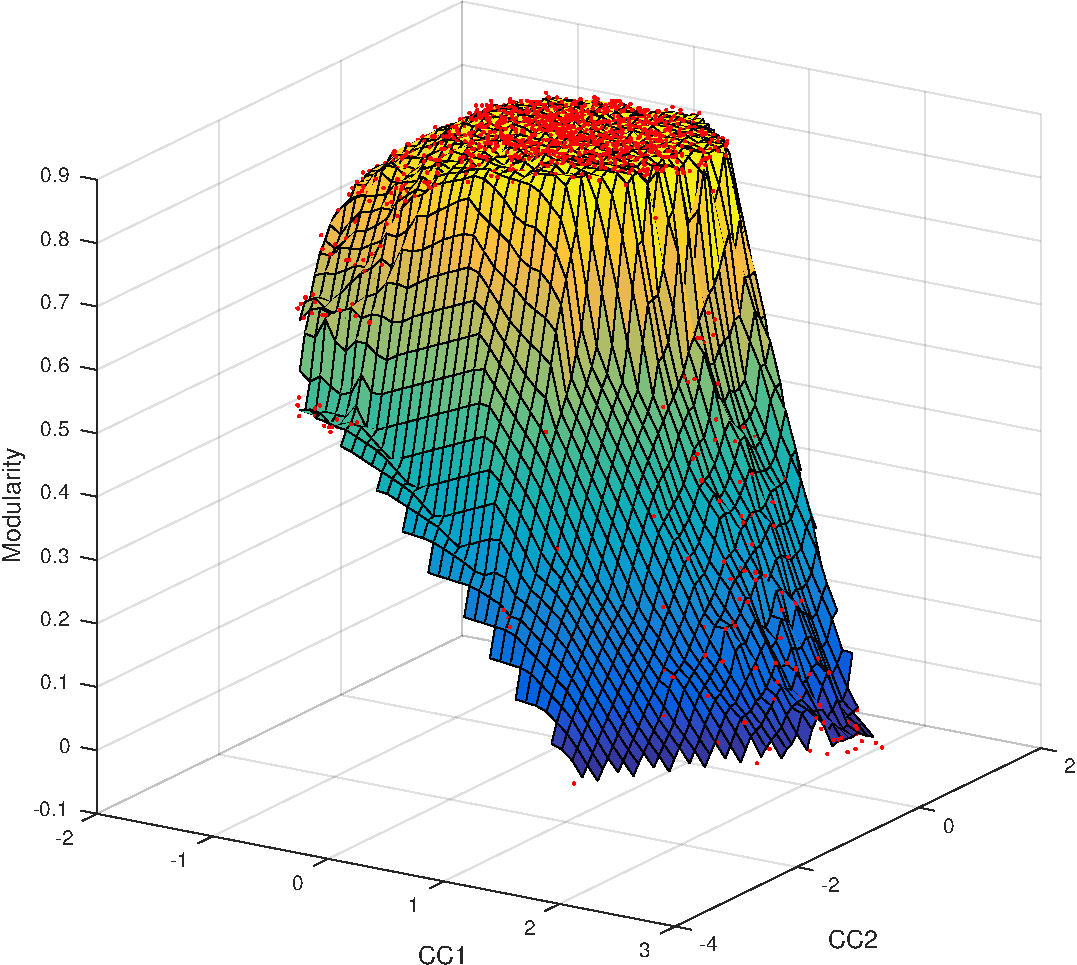
\includegraphics[width=0.75\textwidth]{images/degeneracy_modularity.pdf}
\caption{Degeneracy landscape for Newman's Modularity in a ring of cliques with $r=24$ cliques of $n_r=5$ nodes. The axes CC1 and CC2 are complicated functions of the original partition space computed as to maintain the distance relation between points and their scale is unimportant.}
\label{fig:degeneracylandscape}
\end{figure}

\textcolor{red}{Any quality function suffering from degeneracy of solutions should display an embedded landscape with a plateau of optimal partitions, like the one shown in Figure~\ref{fig:degeneracylandscape}, while in the case of the existence of a distinct global optimum, a sharper peak should be exhibited.
We'll see that recasting the problem of community detection in terms of probability theory, will help in the definition of a quality function showing convex behaviour and uniqueness of the optimum solution.}\todo{CHECK REPHRASE}

Several approaches have been proposed to mitigate the problems that are apparent in Modularity. These include the use of multiple near-optimal solutions to avoid the pitfalls of degeneracy. Moreover a proper choice of the null model may help overcome the fundamental resolution limit.

The issue of degeneracy affects Newman's Modularity $Q^N$ and other quality functions as well.
In this respect, it's clear that choosing the partition with the highest quality value isn't meaningful and a choice that considers all the good partitions at the plateau may be more desirable. 
An optimal partition of the network can then be expressed as a \emph{median} of the solutions over the optimal plateau.
This approach, known as \emph{consensus clustering}, averages local effects of noise during optimization over a large set of solutions.
Consensus clustering is typically based on a meta-algorithm rather than a proper community detection method.
Indeed, given a community detection method, consensus clustering forms an ensemble of optimal solutions from which an association matrix $\mathcal{A}$ is computed, where edges are proportional to the probability that two nodes are connected in the same community. 
Consensus communities are then obtained iteratively by clustering the thresholded association matrix.
The choice of the threshold that makes the association matrix sparser~\cite{lancichinetti2012} is dictated by the properties of the chosen method of community detection itself.
Typically with a judicious choice of the threshold, consensus clustering converges in a few iterations.
The pseudo-code reported in Algorithm~\ref{alg:consensus_clustering} illustrates all the steps of consensus clustering.

\begin{Algorithm}[htb!]
\begin{codebox}
\Procname{\proc{ConsensusClustering}(a graph $G$, a community detection method)}
\li Apply community detection on $G$ for $n_p$ times, yielding $n_p$ partitions.
\li Compute the consensus (association) matrix $\mathcal{A}$ where $\mathcal{A}_{ij}$ is the probability \\that vertex $i$ and $j$ are assigned in the same community over $n_p$ partitions.
\li Threshold the association matrix $\mathcal{A}$ with a parameter $\tau$.
\li Apply community detection on $\mathcal{A}$ for $n_p$ times to yield $n_p$ partitions.
\li If $\mathcal{A}$ is block diagonal (all partitions are equal) stop, else return to 1.
\end{codebox}
\caption{Pseudocode for the implementation of consensus clustering.}
\label{alg:consensus_clustering}
\end{Algorithm}

Although useful to address the degeneracy issue, this approach still suffers from the resolution limit, as the near-optimal optimal solutions which the consensus partition is made of, are resolution-limited per se.

%%%%%%%%%%%%%%%%%%%%%%%%%%%%%%%%%%%%%%%%%%%%%%%%%%%%%%%%
%%%%%%%%%%%%% MODULARITY OPTIMIZATION %%%%%%%%%%%%%%%%%%
%%%%%%%%%%%%%%%%%%%%%%%%%%%%%%%%%%%%%%%%%%%%%%%%%%%%%%%%
\section{Modularity optimization: the Louvain method}\label{sec:louvain_method}
Optimization of fitness function in the additive form of Eq.~\ref{eq:rbspinglass2} is typically performed using the Louvain method~\cite{blondel2008}, a greedy stochastic agglomerative clustering algorithm that works on hierarchical refinements of the network's partitions. The inspiration for this method of community detection is the optimization of Modularity as the algorithm progresses. In the Louvain method of community detection, first small communities are found by optimizing modularity locally on all nodes, then each small community is grouped into one node and the first step is repeated.

This algorithm has become extremely popular in recent years because it is fast, allowing to analyze huge networks with billions of edges~\cite{lancichinetti2009}.
Due to its intrinsic stochastic nature, the Louvain method returns different near-optimal partitions every run and must be typically run thousands of times in order to identify the best solution.
The optimization method is divided in two phases applied recursively as depicted in Figure~\ref{fig:louvain_method}. The first phase is the optimization phase which looks for a locally optimal partition by considering only individual vertex swaps. As in many other greedy algorithms, the community partition is initialized with a single node per community and as many communities as nodes in the input network. Then, based on the chosen cost function, individual nodes are removed from their current community and swapped to the neighboring community which produces the largest positive gain of the cost function.

\begin{figure}[htb!]
\centering
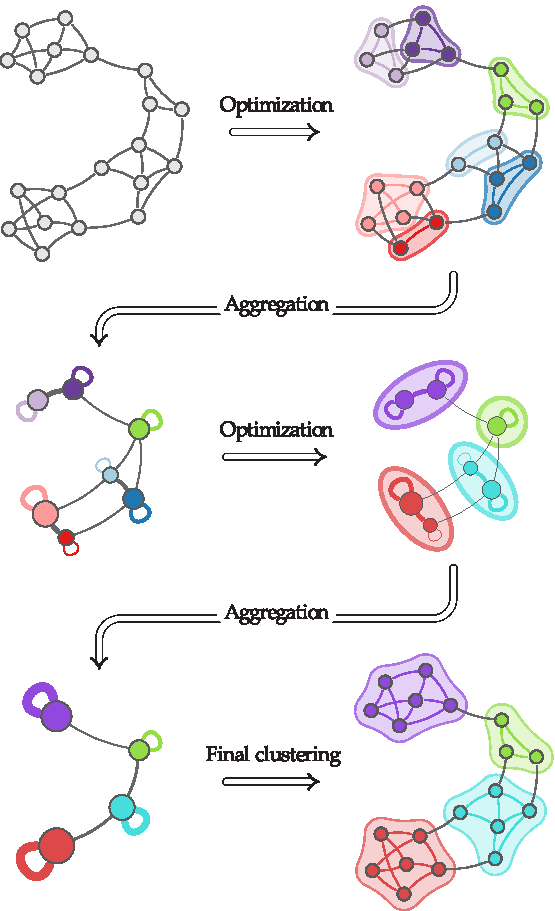
\includegraphics[width=0.6\textwidth]{images/louvain_method.pdf}
\caption{Optimization and aggregation steps with the Louvain method. Figure taken from~\cite{browet2014}.}
\label{fig:louvain_method}
\end{figure}

%%%%%%%%%%%%%%%%%%%%%%%%%%%%%%%%%%%%%%%%%%%%%%%%%%%%%%%%
%%%%%%%%%%%%% SPECTRAL OPTIMIZATION %%%%%%%%%%%%%%%%%%%%
%%%%%%%%%%%%%%%%%%%%%%%%%%%%%%%%%%%%%%%%%%%%%%%%%%%%%%%%
\subsection{Spectral optimization}
Another (and earlier) method to optimize Modularity is the spectral Modularity by Newman. Given the form of Modularity as in Eq.~\ref{eq:newmanmodularityspinglass}, one calls the modularity matrix the quantity $\mathbf{B}=A_{ij} - k_i k_j/2m$. From it, it's possible to obtain an equivalent linear algebra formulation of Modularity that reads:
\begin{equation}\label{eq:newman_spectral}
Q^N = \frac{1}{4m} \mathbf{s}^T \mathbf{B} \mathbf{s}
\end{equation}
where $\mathbf{s}$ is a numerical vector that considers a division of the network in two communities, with values $s_i=+1$ if vertex $i$ belongs to group 1 and $s_i=-1$ if vertex $i$ belongs to group 2. With some manipulations~\cite{newman2006,newman2010book}, the Modularity maximization is turned into an symmetric eigenvalue problem of the form
\begin{equation}
\mathbf{B} \mathbf{s} = \beta \mathbf{s}.
\end{equation}
The group assignment of each node is obtained as the signs of the eigenvector $\mathbf{s}$ corresponding to the greatest eigenvalue $\beta$. Finally, by repeatedly subdividing the network, the optimal Modularity assignment is recovered~\cite{newman2006,newman2010book}.

%%%%%%%%%%%%%%%%%%%%%%%%%%%%%%%%%%%%%%%%%%%%%%%%%%%%%%%%
%%%%%%%%%%%%%%%%%%% CONCLUSIONS %%%%%%%%%%%%%%%%%%%%%%%%
%%%%%%%%%%%%%%%%%%%%%%%%%%%%%%%%%%%%%%%%%%%%%%%%%%%%%%%%
\section{Conclusions}
The modular organization of brain functional connectivity networks has been investigated by a variety of methods and specifically by graph theoretical approaches. The rich repertoire of behavioural and cognitive aspects of everyday life is supported by integration of local processing that is reflected in the functional modules, as identified by a variety of protocols.
Unfortunately Newman's Modularity, the most widely used graph-based method for community detection in FC networks is flawed as it cannot detect modules that are smaller than a certain scale, making impossible to ascertain important details of architectural structure.
The two main drawbacks of Modularity have been introduced namely the resolution limit and its extreme degeneracy, together with analyses that specifically address their origin. In the following chapter I will illustrate how to overcome the limitations imposed by Newman's Modularity with an approach that has its roots in probability theory: Surprise.


\chapter{Beyond the resolution limit in binary networks}\label{chap:beyondresolutionlimitbinarynetworks}
In the last chapter I have introduced the framework of network science used to study brain networks.
I discussed the modular organization of brain networks and the graph theoretical approaches that enabled its study.
I have also shown that graph partitioning methods based on the maximization of global fitness functions, like Newman's Modularity, suffer from a fundamental resolution limit as they fail to detect modules that are smaller than a scale determined by the size of the entire graph.
Furthermore, I explored the effects of this limitation on the study of brain connectivity networks, demonstrating that the resolution limit prevents detection of important details of the brain modular structure, thus hampering the ability to appreciate differences between networks and to assess the topological roles of nodes.

In this chapter I'll show that Surprise, a recently proposed fitness function based on probability theory, does not suffer from these limitations.
I'll introduce Surprise from its theoretical foundations and discuss its properties in details.
Moreover, I'll describe an algorithm for Surprise optimization in binary graphs with an assessment of its performance on benchmark networks.
Surprise maximization in brain co-activation and functional connectivity resting state networks reveals the presence of a rich structure of heterogeneously distributed modules, and differences in networks' partitions that are undetectable by resolution-limited methods.
Moreover, Surprise leads to a more accurate identification of the network's connector hubs, the elements that integrate the brain modules into a cohesive structure.

%%%%%%%%%%%%%%%%%%%%%%%%%%%%%%%%%%%%%%%%%%%%%%%%%%%%%%%%%%%%%%%%%%%%%%%%%%%%%%%%%%%%%%%%%
%%%%%%%%%%%%%% PROBABILISTIC APPROACH TO CLUSTERING IN BINARY NETWORKS %%%%%%%%%%%%%%%%%%
%%%%%%%%%%%%%%%%%%%%%%%%%%%%%%%%%%%%%%%%%%%%%%%%%%%%%%%%%%%%%%%%%%%%%%%%%%%%%%%%%%%%%%%%%
\section{Probabilistic approach to clustering in binary networks}\label{sec:probability_clustering}
The spin-glass based additive quality functions described in the previous chapter, including Newman's Modularity, measure the deviation between the fraction of edges falling within modules and the null model. In any case though, they assess the statistical significance of this deviation.
In other terms, no spin-glass based quality function is telling us the level of statistical confidence at which one should discard the null hypothesis that the observed fraction of edges inside a community is the same as the one expected from a given null model.

To address this question, one should instead compute probabilities, as they are the natural way to measure statistical significance.
Specifically, given a node induced subgraph (a community), one is interested in computing the probability to find another subgraph having more internal edges than the observed one: the lesser the value, the more significant is the community in exam.

More precisely, the problem can be expressed as in the following: given a subgraph, what is the probability of observing another subgraph with a larger number of internal edges drawn from a random graph with a given density?
This question can be answered by the urn model in classical probability theory. The reason is clear if one imagines that each pair of nodes is a marble, which is one color if the nodes are connected by a link and the other color if they are not.
A number of marbles is drawn from an urn without replacement and the probability of observing a given number of marbles of one specific color is calculated by means of the hypergeometric law.
When applied to clustering, the problem corresponds to the calculation of the probability to observe a fixed number of internal edges in a randomly drawn set of nodes defining a community.
For example, suppose that one draws a subgraph with $n_c$ nodes, $p_c$ pairs of nodes and $m_c$ edges from a graph with $n$ nodes, $p$ pairs of nodes and $m$ edges (see Section for the notation~\ref{sec:clustering}).
As indicated by the urn model, the probability to observe exactly $m_c$ internal edges is given by:
\begin{equation}\label{eq:subgraph_probability}
\Pr[i=m_c] = \frac{\binom{m}{i}\binom{p-m}{p_c-i} }{\binom{p}{p_c}} = \frac{\binom{p_c}{i} \binom{p-p_c}{m-i}}{\binom{p}{m}}
\end{equation}
where the last equality is because of the Vandermonde identity~\cite{feller1968}.
The probability in Eq.~\ref{eq:subgraph_probability} is simply understood in terms of urn model as there are $\binom{p_c}{i}$ ways of choosing exactly $i$ black marbles from a population of $p_c$ black marbles, $\binom{p-p_c}{m-i}$ ways of choosing $(m-i)$ white marbles from a population of $(p-p_c)$ white marbles and a total possible number of combinations of $m$ marbles taken from a population of $p$ of them. Figure~\ref{fig:subgraphconditionalprobability} shows an example where the probability of randomly picking the subgraph $\mathcal{G}$ from the graph $G$ is computed by means of the urn model.
\begin{figure}[htb]
\centering
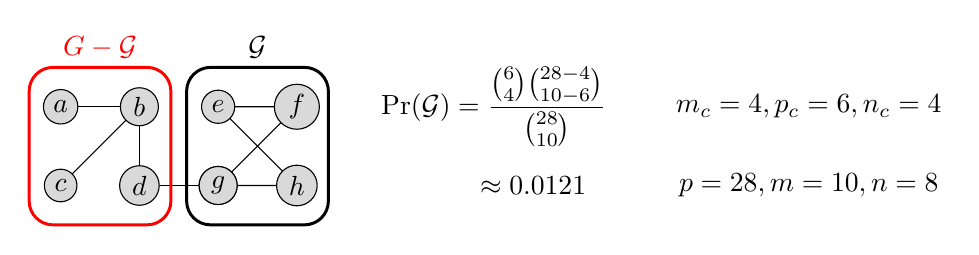
\begin{tikzpicture}
%\draw[help lines,step=1] (-4,-4) grid (8,4);
\draw [rectangle, black, draw, rounded corners=2ex,line width=0.25ex] (1.6,-0.5) rectangle (3.4,1.5);

\draw (1,0) -- (3,0);
\draw (2,1) -- (3,1) -- (2,0) -- (3,0) -- cycle;
\node [fill=gray!30, radius=1ex, draw, circle, inner sep=2pt] at (2,1) {$e$};
\node [fill=gray!30, radius=1ex, draw, circle, inner sep=2pt] at (3,1) {$f$};
\node [fill=gray!30, radius=1ex, draw, circle, inner sep=2pt] at (2,0) {$g$};
\node [fill=gray!30, radius=1ex, draw, circle, inner sep=2pt] at (2,0) {$g$};
\node [fill=gray!30, radius=1ex, draw, circle, inner sep=2pt] at (3,0) {$h$};
\draw (0,1) -- (1,1);
\draw (1,1) -- (1,0);
\draw (1,0) -- (1,1);
\draw (1,1) -- (0,0);
\node [fill=gray!30, radius=1ex, draw, circle, inner sep=2pt] at (0,1) {$a$};
\node [fill=gray!30, radius=1ex, draw, circle, inner sep=2pt] at (1,1) {$b$};
\node [fill=gray!30, radius=1ex, draw, circle, inner sep=2pt] at (0,0) {$c$};
\node [fill=gray!30, radius=1ex, draw, circle, inner sep=2pt] at (1,0) {$d$};
\node at (2.5,1.75) {$\mathcal{G}$};
\node at (0.5,1.75) {{\color{red}$G-\mathcal{G}$}};
\draw [rectangle, red, draw, rounded corners=2ex,line width=0.25ex] (-0.4,-0.5) rectangle (1.4,1.5);
\node [] at (5.5,1) {$\Pr(\mathcal{G}) = \dfrac{\binom{6}{4} \binom{28-4}{10-6}}{\binom{28}{10}}$};
\node [] at (6.0,0) {$\approx 0.0121$};

\node [] at (9.5,1) {$m_c=4,p_c=6,n_c=4$};
\node [] at (9.5,0) {$p=28,m=10,n=8$};
\end{tikzpicture}
\caption{Probability for the subgraph $\mathcal{G}=(\mathcal{V},\mathcal{E})$ where $\mathcal{V}=\{e,f,g,h\}$ and $\mathcal{E}=\{(e,f),(f,g),(g,h),(e,h)\}$ to be randomly drawn from the graph $G$.}
\label{fig:subgraphconditionalprobability}
\end{figure}
As the probability of observing $i$ or more internal edges, is given by the sum of the probabilities of observing exactly $i$,$i+1$,$i+2$ etc. internal edges, summing on $i$ yields the probability of getting \emph{at least} $m_c$ white marbles:
\begin{equation}\label{eq:subgraph_probability_marginalized}
\Pr[ m_c \geq i ] = \sum\limits_{i=m_c}^{m} \frac{\binom{p_c}{i} \binom{p-p_c}{m-i}}{\binom{p}{m}}
\end{equation}

In this last equation we are considering the probability of randomly drawing a subgraph with $m_c$ or more internal edges over the set of all random subgraphs with $n$ nodes and exactly $m$ edges as in the $G_{nm}$ model described in section~\ref{sec:models_random_graph}. Indeed, the denominator $\binom{p}{m}$ in Equation~\ref{eq:subgraph_probability_marginalized} represent the possible number of graphs with $p$ pairs of nodes and $m$ edges. 

%%%%%%%%%%%%%%%%%%%%%%%%%%%%%%%%%%%%%%%%%%
%%%%%%%%%%%%%% SURPRISE %%%%%%%%%%%%%%%%%%
%%%%%%%%%%%%%%%%%%%%%%%%%%%%%%%%%%%%%%%%%%
\section{Surprise}
The intuition captured by Eq.~\ref{eq:subgraph_probability_marginalized} is very close to a quality function dubbed \emph{Surprise}, firstly introduced in a seminal paper by Aldecoa and Marin~\cite{aldecoa2011}.
Yet, to the best of my knowledge, this clearer theoretical motivation did not appear in any other works.
If one considers as the random subgraph that is drawn from the $G_{n,m}$ set, a subgraph with at least $m_\zeta=\sum_c m_c$ internal edges and $p_\zeta=\sum_c p_c$ pairs of edges, then this subgraph represents a whole clustering.
In this case, the definition given in Eq.~\ref{eq:subgraph_probability_marginalized} and the definition given in~\cite{aldecoa2011} are perfectly corresponding.
Indeed, for a partition $\zeta$, the probability that a subgraph $\mathcal{G}$ randomly drawn from the set $G_{nm}$ has at least $m_\zeta$ intracluster edges and $p_\zeta$ intracluster pairs is modeled after the inverse cumulative hypergeometric distribution, exactly as in~\ref{eq:subgraph_probability_marginalized}.
Here and in the rest of the work, the quality function \emph{Surprise} is therefore expressed by the following definition:
\begin{equation}\label{eq:surprise}
S(\zeta) := \sum_{i = m_\zeta}^m \dfrac{\binom{p_\zeta}{i} \binom{p-p_\zeta}{m-i} }{\binom{p}{m}}
\end{equation}

Surprise computes the probability to (surprisingly) observe at least as many internal edges as within the proposed partition in a uniform random graph.
As mentioned, model in Eq.~\ref{eq:surprise} corresponds to an urn model without reinsertion, where $S$ is the probability of extracting at least $m_\zeta$ white balls out of $m$ trials from an urn containing $p_\zeta$ white balls and $p-p_\zeta$ black balls.
Intuitively, the lower $S(\zeta)$, the better the clustering. Optimal partitions with respect to $S$ are those with the highest number of intracluster edges and the smallest number of intracluster pairs. 

Differently from Modularity, $S(\zeta)=1$ both for the partition where every node is in a separated community ($|\zeta|=n$,$p_\zeta=0$,$m_\zeta=0$) and for the partition that entails all nodes into a single group ($|\zeta|=1$,$p_\zeta=p$,$m_\zeta=m$) as is evident from its formulation in terms of urn model.
Indeed, as Newman's Modularity is zero when $|\zeta|=1$, and different from zero in the case $|\zeta|=n$.
In terms of Surprise both the extreme partitions are instead equally uninformative and assigned to $S=1$ (or equivalently $\hat{S}=0$).
Indeed, for the case of a single community comprising all nodes, the probability of observing a number of intracluster edges greater or equal than the number of edges is one. On the other hand, if the partitioning has zero intracluster edges as for the case of $n$ separate communities, the probability to observe more than zero intracluster edges is still one.

It should be noted that, due to numerical precision problems in the evaluation of large binomial coefficients, $\hat{S}(\zeta) := -\log_{10}S(\zeta)$ is often taken as measure of quality of the partition, which is totally equivalent with respect to optimum solutions, where higher values correspond to better clustering.
Different authors~\cite{arnauVMarsS2005,fleck2014} refer to $S$ as Surprise, whereas others~\cite{aldecoa2011,aldecoa2013} use $\hat{S}$. Hereafter I stick to the notation of~\cite{fleck2014} where Surprise is indicated as $S$ defined in Eq.~\ref{eq:surprise} and indicate $\hat{S}$ where needed.

%%%%%%%%%%%%%%%%%%%%%%%%%%%%%%%%%%%%%%%%%%%%%%%%%%%%%%%%%%%%%%
%%%%%%%%%%%%% STATISTICAL TEST INTERPRETATION %%%%%%%%%%%%%%%%
%%%%%%%%%%%%%%%%%%%%%%%%%%%%%%%%%%%%%%%%%%%%%%%%%%%%%%%%%%%%%%
\subsection{Statistical test interpretation}
\label{sec:surprisefishertest}
Surprise considers the problem of community detection as the one of making the intracluster density as further as possible from the global density in statistical terms.
In this sense, it's worth noting that $S$ is \emph{p}-value of a one-tailed Fisher exact-test where one is asking how confidently should reject the null hypothesis $H_0$ that the intracluster density is the same as the graph density.
It turns indeed out that this problem has an equivalent description in statistics, where one seeks to maximize the \emph{odds-ratio} of the $2 \times 2$ contingency table defined in Table~\ref{tab:contingency_table}.

The Fisher exact test implemented by Surprise is, as its name states, exact as long as the contingency table keeps the row and column totals fixed, and it can therefore be used regardless of the sample characteristics.
A simpler $\chi^2$ statistic can be used when the elements of the contingency table are large enough, although only an approximation of the \emph{p}-value can be obtained.
In this case it's possible to tackle the problem of computation of $S$ by means of odds-ratio.
Precisely, the \emph{normalized log odds-ratio} is computed as: 
\begin{equation}
\log(\textrm{OR}) = \log\left( \frac{m_\zeta(p-m-p_\zeta+m_\zeta)}{(m-m_\zeta)(p_\zeta-m_\zeta)} \right ),
\end{equation}
and in the asymptotic case, Surprise is equal to the probability:
\begin{equation}\label{eq:prob_or_se}
\Pr\left(z < -\frac{|\log\textrm{OR})|}{SE} \right)
\end{equation}
where $z$ is a random variable with standard normal distribution $z \approx \mathcal{N}(0,1)$ and $SE$ is the standard error of the odds-ratio, approximately computed as 
\begin{equation}
SE=\sqrt{\frac{1}{m_\zeta} + \frac{1}{(p_\zeta-m_\zeta)} + \frac{1}{(m-m_\zeta)} + \frac{1}{(p - m - p_\zeta + m_\zeta)}}.
\end{equation}
Although not interesting in the case of binary graphs, Equation~\ref{eq:prob_or_se} is telling us that in developing a version of Surprise that will keep into account weighted graphs, we should in some way rely on its asymptotic distribution.

\begin{table}[htb!]
\centering
\begin{tabular}{|c|c|c|c|}
\hline
 & Drawn & Not drawn & \textbf{Total}\\
\hline
Intracluster & $m_\zeta$ & $p_\zeta-m_\zeta$ & $p_\zeta$\\
\hline
Intercluster & $m-m_\zeta$ & $p-m-p_\zeta+m_\zeta$ & $p-p_\zeta$ \\
\hline
\textbf{Total} & $m$ & $p-m$ & $p$ \\
\hline
\end{tabular}
\caption{Contingency table for the urn model.}
\label{tab:contingency_table}
\end{table}

%%%%%%%%%%%%%%%%%%%%%%%%%%%%%%%%%%%%%%%%%%%%%%%%%%%%%%%%%%%%%%%%%%%%%%%%%%%%%%%%%%%%
%%%%%%%%%%%%%%%%%%%%%%%%%%%% GENERAL PROPERTIES OF SURPRISE %%%%%%%%%%%%%%%%%%%%%%%%
%%%%%%%%%%%%%%%%%%%%%%%%%%%%%%%%%%%%%%%%%%%%%%%%%%%%%%%%%%%%%%%%%%%%%%%%%%%%%%%%%%%%
\subsection{General properties of Surprise}
As noted by~\cite{fleck2014}, for a given graph, $m$ and $p$ are fixed so $S(\zeta)$ is depending only on the number of intracluster edges $m_\zeta$ and intracluster pairs $p_\zeta$, namely $S:=S(m_\zeta,p_\zeta)$.
In establishing the domain of validity of $(m,p,m_\zeta,p_\zeta)$ the urn model is of help. A valid clustering $\zeta$ of mutually disjoint communities automatically satisfies intuitive but important requirements:
\begin{obs}
It's impossible to draw more white balls than the white balls contained in the urn, therefore $p_\zeta \geq m_\zeta$.
\end{obs}
\begin{obs}
It's impossible to have more white balls than total number of drawn balls, therefore $m\geq m_\zeta$.
\end{obs}
\begin{obs}
It's impossible to draw more black balls than the black balls contained in the urn, therefore $p-p_\zeta \geq m-m_\zeta$.
\end{obs}
All valid clusterings are enclosed inside the domain $\mathcal{L}$ defined as from these last three observation:
\begin{equation}
\mathcal{L} := \{ ( m_\zeta,p_\zeta) \; | m_\zeta > 0 \land p_\zeta \geq m_\zeta \land m \geq m_\zeta \land p-m > p_\zeta - m_\zeta \}
\end{equation}
The urn models gives other three important properties, indicating that Surprise is a convex function inside the domain of validity of its variables. Specifically as shown in~\cite{fleck2014} three inequalities apply for Surprise and for the urn model in general.
\begin{props}\label{prop:prop1}
\label{list:surprise_properties} It's less probable to draw at least $m_\zeta+1$ than $m_\zeta$ white balls if the urn contains the same number of $p_\zeta$ white balls, therefore $S(m_\zeta+1,p_\zeta) < S(m_\zeta,p_\zeta)$.
\end{props}
\begin{props}\label{prop:prop2}
It's less probable to draw at least $m_\zeta$ white balls if the urn has one white balls less, therefore $S(m_\zeta,p_\zeta-1) < S(m_\zeta,p_\zeta)$.
\end{props}
\begin{props}\label{prop:prop3}
It's less probable to draw at least $m_\zeta+1$ white balls if the urn has $p_\zeta+1$ white balls, than drawing at least $m_\zeta$ white balls if the urn has $p_\zeta$ white balls, therefore $S(m_\zeta+1,p_\zeta+1) < S(m_\zeta,p_\zeta)$.
\end{props}
The scheme in Figure~\ref{fig:surprisebehaviour} shows the order relation between the elements of the three aforementioned inequalities.
\begin{figure}[htb]
\centering
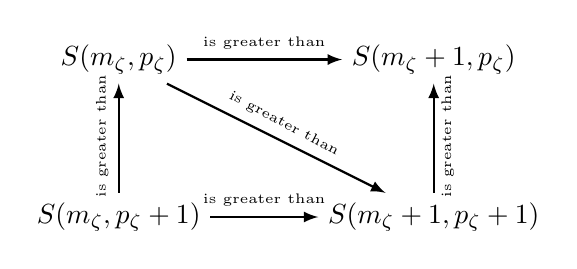
\begin{tikzpicture}
  \node[] (S00) at (0,0) {$S(m_\zeta,p_\zeta)$};
  \node[] (S10) at (4,0) {$S(m_\zeta+1,p_\zeta)$};
  \node[] (S01) at (0,-2) {$S(m_\zeta,p_\zeta+1)$};
  \node[] (S11) at (4,-2) {$S(m_\zeta+1,p_\zeta+1)$};
  \draw[->,thick,>=latex] (S00) -- node[anchor=south] {\tiny{is greater than}} (S10);
  \draw[->,thick,>=latex] (S01) -- node[anchor=south] {\tiny{is greater than}} (S11);
  \draw[->,thick,>=latex] (S11) -- node[anchor=west,xshift=5,yshift=-25,rotate=90] {\tiny{is greater than}} (S10);
  \draw[->, thick,>=latex] (S00) -- node[anchor=south,rotate=-28] {\tiny{is greater than}} (S11);
  \draw[->,thick,>=latex] (S01) -- node[anchor=west,xshift=-6,yshift=-25,rotate=90] {\tiny{is greater than}} (S00);
\end{tikzpicture}
\caption{Behaviour of the landscape of Surprise $S$.}
\label{fig:surprisebehaviour}
\end{figure}

A fourth inequality $S(m_\zeta,p_\zeta+1)>S(m_\zeta+1,p_\zeta)$ is implicit by looking at the behaviour of $S(\zeta)$ for a given graph. 
The scheme in Figure~\ref{fig:surprisebehaviour} allows to rank the values of Surprise in relation to changes in $m_\zeta$ and $p_\zeta$.
It's to easy verify that $S$ satisfies the following strict order relation:
\begin{equation}\label{eq:surpriseorderrelation}
S(m_\zeta+1,p_\zeta)<S(m_\zeta+1,p_\zeta+1)<S(m_\zeta,p_\zeta)<S(m_\zeta,p_\zeta+1).
\end{equation}
This property led me to the observation that Surprise $S$ is a monotonically decreasing function (increasing $\hat{S}$) of $m_\zeta$ and monotonically increasing function (decreasing $\hat{S}$) of $p_\zeta$ in the convex interval $\mathcal{L}$.
Moreover, from Figure~\ref{fig:surprisebehaviour} follows that optimal solutions with respect to $S$ are Pareto-optimal with respect to maximizing $m_\zeta$ and minimizing $p_\zeta$.
In other words, a partition that is optimum with respect to Surprise is such that no further increment in $m_\zeta$ leads to a decrement in $p_\zeta$ that has higher $\hat{S}$.
The Pareto optimality of optimum Surprise partitions, implies that a perturbation of $\delta m_\zeta, \delta p_\zeta$ leads to a change in Surprise such that it monotonically decreases if and only if $\delta m_\zeta > \delta p_\zeta$, precisely:
\begin{equation}\label{eq:resolution_limit_condition}
S(m_\zeta + \delta_{m_\zeta}, p_\zeta + \delta_{p_\zeta}) < S(m_\zeta,p_\zeta) \iff \delta_{m_\zeta} \geq \delta_{p_\zeta}.
\end{equation}

%% \begin{figure}[htb!]
%% \centering
%% \begin{tikzpicture}[scale=0.8, every node/.style={scale=0.8}]
%% \def \S {1};
%% \def \W {11};
%% \def \H {7};
%% \node[anchor=south west, inner sep=0mm] at (0,0) { 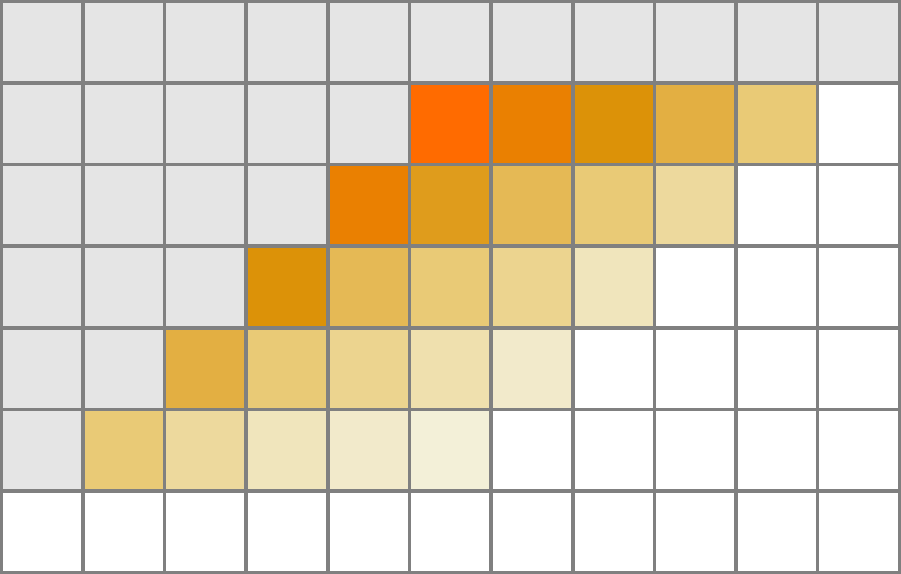
\includegraphics[width=\W cm]{images/plot_surprise_pareto.pdf}};
%% \node[anchor=south] at (\W /2,\H +0.25) {$\hat{S}=-\log_{10}(S(m_\zeta,p_\zeta$, $m=10$,$p=15$))};
%% %\draw[help lines,xstep=1.0,ystep=1.0] (0,0) grid (\W,\H);
%% \foreach \x in {1,...,\W } {\node [anchor=north] at (\x-0.5,0) {$\x$}; }
%% \node[anchor=north] at (\W/2,-0.5){$p_\zeta$};
%% \foreach \y in {1,...,\H} {\node [anchor=east] at (0 ,\y-0.5) {$\y$}; }
%% \node[anchor=east] at (-0.5,\H/2){$m_\zeta$};
%% %\node[rectangle,fill=black!10,draw=black,rounded corners=0.1cm] at (\W+1.5,\H-0.5) {$m_{\zeta},p_\zeta \not \subset \mathcal{L}$};
%% \end{tikzpicture}
%% \caption{Pareto optimality of Surprise (here $\hat{S}$ is represented) on a trivial graph with $n=6$ nodes and $m=7$ edges. No increment in $m_\zeta$ leads to a decrement in $p_\zeta$ that has higher $\hat{S}$. Here Surprise is optimal for $m_\zeta=6,p_\zeta=6$.}
%% \label{fig:pareto_optimality_surprise}
%% \end{figure}
%% \todo[inline]{CONTROLLARE FIGURA PROBABILMENTE SBAGLIATA PERCHE MZETA>M!!!}

The result in Eq.\ref{eq:resolution_limit_condition} is of great help in designing optimization algorithms as every move that increase the intracluster edges more than intracluster pairs is good, while moves that increase intracluster pairs more than intracluster edges must be ignored, therefore sparing time for the computation of Surprise. Additionally, Eq.~\ref{eq:resolution_limit_condition} is useful when analyzing the onset of the resolution limit for different models.
In the next sections I will show to what extent Surprise is affected by the resolution limit for Surprise, to show with convincing theoretical arguments that $S$ is nearly resolution-limit-free in Traag's sense~\cite{traag2015}.

%%%%%%%%%%%%%%%%%%%%%%%%%%%%%%%%%%%%%%%%%%%%%%%%%%%%%%%%%%%%%%
%%%%%%%%%%%% RESOLUTION LIMIT AND SURPRISE %%%%%%%%%%%%%%%%%%%
%%%%%%%%%%%%%%%%%%%%%%%%%%%%%%%%%%%%%%%%%%%%%%%%%%%%%%%%%%%%%%
\section{Resolution limit and Surprise}
Unfortunately, the resolution limit is an intrinsic feature of many quality functions, and there appears to be a ``narrow scope to resolution-limit-free methods''~\cite{traag2015}.
Surprise has been shown to outperform other network partitioning methods in the detection of small features within large graphs, but the extent to which it suffered from the resolution limit was unknown~\cite{aldecoa2011,aldecoa2013}, until our work~\cite{nicolini2016}.

Aldecoa~\cite{aldecoa2011}, pointed out that while Modularity-based methods define a community as a region with an unexpectedly high density of links with respect to the global characteristics of the network, Surprise weights the number of actual intracluster edges against the maximum number of links given the nodes in the clusters.
Hence, Surprise is able to discriminate local subnetworks whose internal density is close to that of a clique independently of their size.

In order to assess the extent to which Surprise is affected by the resolution limit, I directly compared Newman's Modularity and Surprise in the example of Fortunato and Barthelemy illustrated in the previous chapter in Figure~\ref{fig:figure_1_barthelemy}. Already for $m_{12} = 1$, i.e. when the two cliques $G_1$ and $G_2$ were connected by only one edge, $Q^N$ showed sign inversion for $m_0 \approx 200$, meaning that it was beneficial for Modularity to merge two cliques.
In this same example, Surprise never merges cliques, as shown in Figure~\ref{fig:barthelemy_surprise}.

\begin{figure}[htb!]
\centering
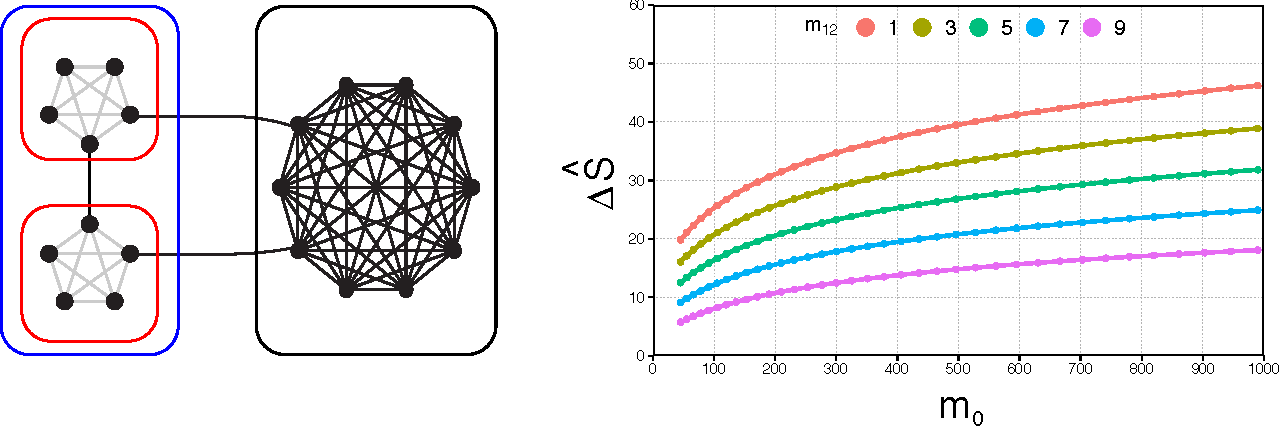
\includegraphics[width=1.0\textwidth]{images/barthelemy_surprise.pdf}
\caption{Difference in $\hat{S}$ between the partition where the two cliques are separated (red) and the partition where the two cliques are merged (blue), as in the benchmark network of Fortunato and Barthelemy. As the quantity $\Delta \hat{S}$ is always positive, Surprise is never going to merge cliques, independently from other global parameters. Adapted from Nicolini and Bifone~\cite{nicolini2016}.}
\label{fig:barthelemy_surprise}
\end{figure}

Figure~\ref{fig:barthelemy_surprise} shows that Surprise does not suffer from the resolution limit at least in this specific case.
Indeed, $\Delta \hat{S}$ is always positive and grows monotonically with increasing $m_0$. 
Hence, the two cliques $G_1$ and $G_2$ are always resolved by Surprise as separate communities independently of the network size, and also in the presence of some ``fuzziness'', i.e. when $m_{12}>1$ and the two cliques are connected by more than one edge.
In order to assess whether this behavior reflects a general property of Surprise, or is incidental to this particular example, I have also studied a generalization of Fortunato and Barthelemy's model.

A consequence of the definition of a resolution limit free quality function in Traag's sense, is that such method will never depend on the size of the network to merge cliques in a graph comprising $r$ cliques of $n_r$ nodes connected in a ring structure as in Figure~\ref{fig:traag_ring_of_cliques} (often called the ``ring of cliques'' model).
This observation prompted me to explore the behavior of $\hat{S}$ in the ring of cliques model graph, as an extension of Fortunato and Barthelemy's model.
Interestingly, given its two-variables formulation, Surprise optimization can be seen as a multiobjective optimization problem where one seeks to minimize the intracluster pairs while maximizing the number of intracluster edges.
With increasing graph size, the computational problem of calculating $\hat{S}$ for every possible partition becomes rapidly intractable (maximization of $S$ is NP hard)~\cite{fleck2014}.
However, as explained before and pointed out by Fleck et al.~\cite{fleck2014}, the Surprise optimal clustering must be Pareto optimal with respect to minimizing $p_\zeta$ and maximizing $m_\zeta$, i.e. any further improvement in one of the two variables must occur at the expense of the other.

In this sense, the problem of Surprise optimization is shown to be equivalent to a linear program~\cite{fleck2014}, where one seeks to minimize $p_\zeta$ while keeping $m_\zeta$ equal to a constant $h$ from $1$ to $m$, choosing then among the resulting $m$ clusterings, the one that maximizes $\hat{S}$.
Hence, to delineate the Pareto frontier in the $(m_\zeta,p_\zeta)$ space, we need to solve $m$ integer linear programs (ILP) in the form:
\begin{align}\label{eq:surprise_ilp}
\textrm{minimize} \sum_{\{i,j\} \in \binom{V}{2}} \mathcal{X}_{ij} \nonumber \\
\textrm{s.t.} \quad \mathcal{X}_{ij} \in \{0,1 \} \nonumber \\
\quad \mathcal{X}_{ik} + \mathcal{X}_{ki} - \mathcal{X}_{ij} \leq 1 \nonumber \\
\sum_{\{i,j\} \in E} \mathcal{X}_{ij}=h \nonumber
\end{align}
where $\mathcal{X}_{ij}$, equivalent to $\delta(\sigma_i, \sigma_j)$, are a set of $\binom{n}{2}$ binary variables corresponding to vertex pairs, with the interpretation that $\mathcal{X}_{ij}=1$ if vertex $i$ and vertex $j$ are in the same community. The alternative objective function $\sum_{ij}\mathcal{X}_{ij}$ measures the number of intracluster pairs $p_\zeta$, while the number of intracluster edges $m_\zeta=\sum_{ij \in E} \mathcal{X}_{ij}$ was set equal to a fixed $h \in [0,m]$. The remaining constraints are necessary in order to ensure transitivity, i.e. if nodes $i$ and $j$ are in the same community, nodes $i$ and $k$ are in the same community, then nodes $j$ and $k$ share the same community too. 
Figure~\ref{fig:ring_cliques_pareto} shows the Pareto frontier for a ring of cliques where I independently varied the number of cliques $r$ and the number of nodes $n$ in every clique\footnote{Linear programs were solved using the Python interfaces of Gurobi 5.7.3 on Linux (Gurobi Optimizer Version 5.7, Gurobi Optimization, Inc., Houston, Texas, United States).}.
As $\hat{S}$ reaches its minimum (zero) both in the case where all nodes are separated communities ($p_\zeta=0$) or when a single community entails all nodes ($p_\zeta=p$), Figure~\ref{fig:ring_cliques_surprise} shows monotonically increasing Surprise along the frontier with increasing $p_\zeta$ up to the Surprise optimum, indicated by black circles in the Pareto front of Figure~\ref{fig:ring_cliques_pareto}, whereas the corresponding partition identified each clique as a separate community.
Importantly, in the range of parameters I have investigated, Surprise optimization never merged cliques in the ring of cliques, independently of the size of the graph, and behaved as a Traag's resolution-limit free method.

\begin{figure}[htb!]
\centering
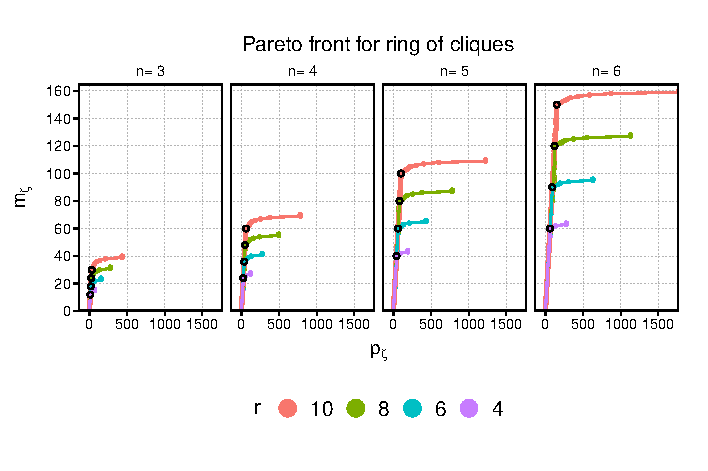
\includegraphics[width=0.8\textwidth]{images/ring_cliques_pareto.pdf}
\caption{Pareto front for a ring of cliques graph. Optimal solutions with respect to Surprise are indicated as small black dots. Adapted from Nicolini and Bifone~\cite{nicolini2016}.}
\label{fig:ring_cliques_pareto}
\end{figure}
\begin{figure}[htb!]
\centering
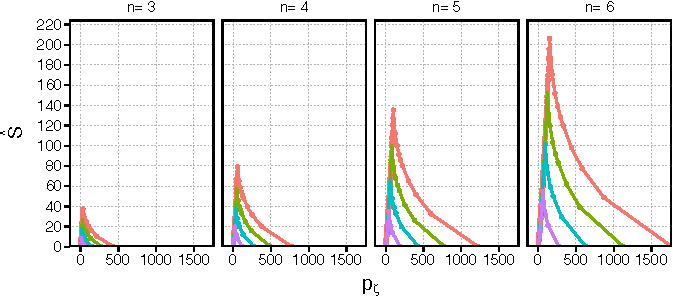
\includegraphics[width=0.8\textwidth]{images/ring_cliques_surprise.pdf}
\caption{Surprise $\hat{S}$ for a ring of cliques graph at different levels of $p_\zeta$ for corresponding solutions at fixed $m_\zeta$. The peak of $\hat{S} $is always reached at $p_\zeta$ when the modules entail single cliques separately. Adapted from Nicolini and Bifone~\cite{nicolini2016}.}
\label{fig:ring_cliques_surprise}
\end{figure}
While it is likely that this property is quite general and can be extended to every ring of cliques, an analytical demonstration is hampered by the non-additivity of the Surprise function.
Nonetheless, the size of the graphs explored numerically is quite typical of brain-connectivity networks and I felt encouraged to apply Surprise maximization to the study of the community structure of the brain.

%%%%%%%%%%%%%%%%%%%%%%%%%%%%%%%%%%%%%%%%%%%%%%%%%%%%%%%%%%%%%%%%%%%%%%%%%%%%%%%%%%%%
%%%%%%%%%%%%%%%%%%%%%%% DEGENERACY OF SURPRISE  %%%%%%%%%%%%%%%%%%%%%%%%%%%%%%%%%%%%
%%%%%%%%%%%%%%%%%%%%%%%%%%%%%%%%%%%%%%%%%%%%%%%%%%%%%%%%%%%%%%%%%%%%%%%%%%%%%%%%%%%%
\section{Degeneracy of Surprise}\label{sec:degeneracy_surprise}
Interestingly, the maximum value of Surprise for given $(m_\zeta,p_\zeta)$ is sharply peaked and very different from other partitions, indicating that at least in this case Surprise shows no degeneracy of optimal solutions, as instead shown for Modularity in Section~\ref{sec:degeneracy}.
This observation led us to investigate to what extent Surprise is affected by the degeneracy problem.
We repeated the procedure indicated in section~\ref{sec:degeneracy}, where I embedded the complex landscape of partitions in a three dimensional space in order to show whether optimal Surprise solutions group in a large plateau of high Surprise values or not. The global optimum is a sharply distinct partition, sitting on top of the embedded manifold, as illustrated in Figure~\ref{fig:degeneracy_surprise}.
\todo{mettere conclusioni degeneracy}
\begin{figure}[ht]
\centering
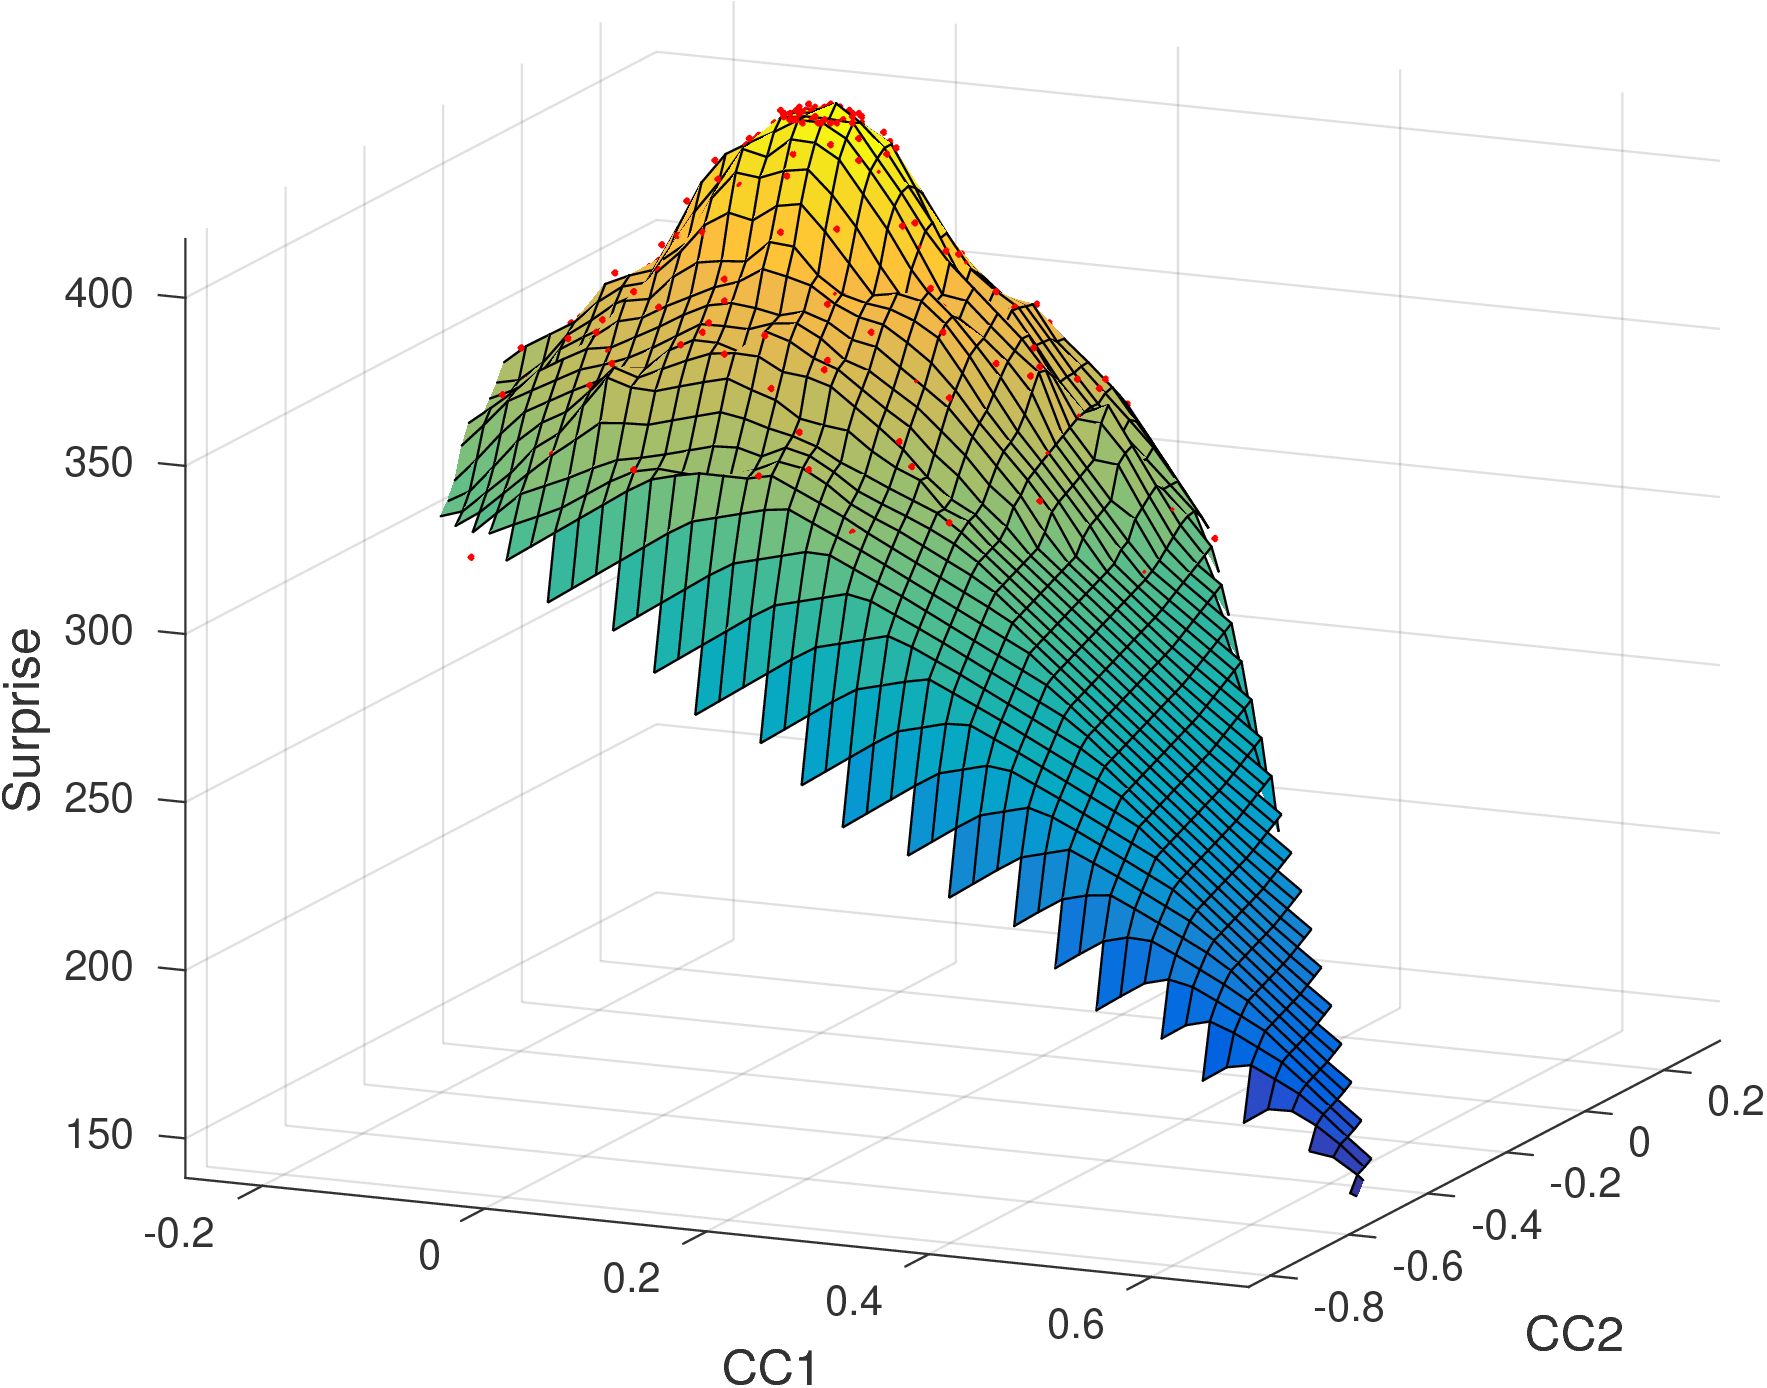
\includegraphics[height=0.4\textwidth]{images/degeneracy_surprise_n_5_c_24.png}\hfill
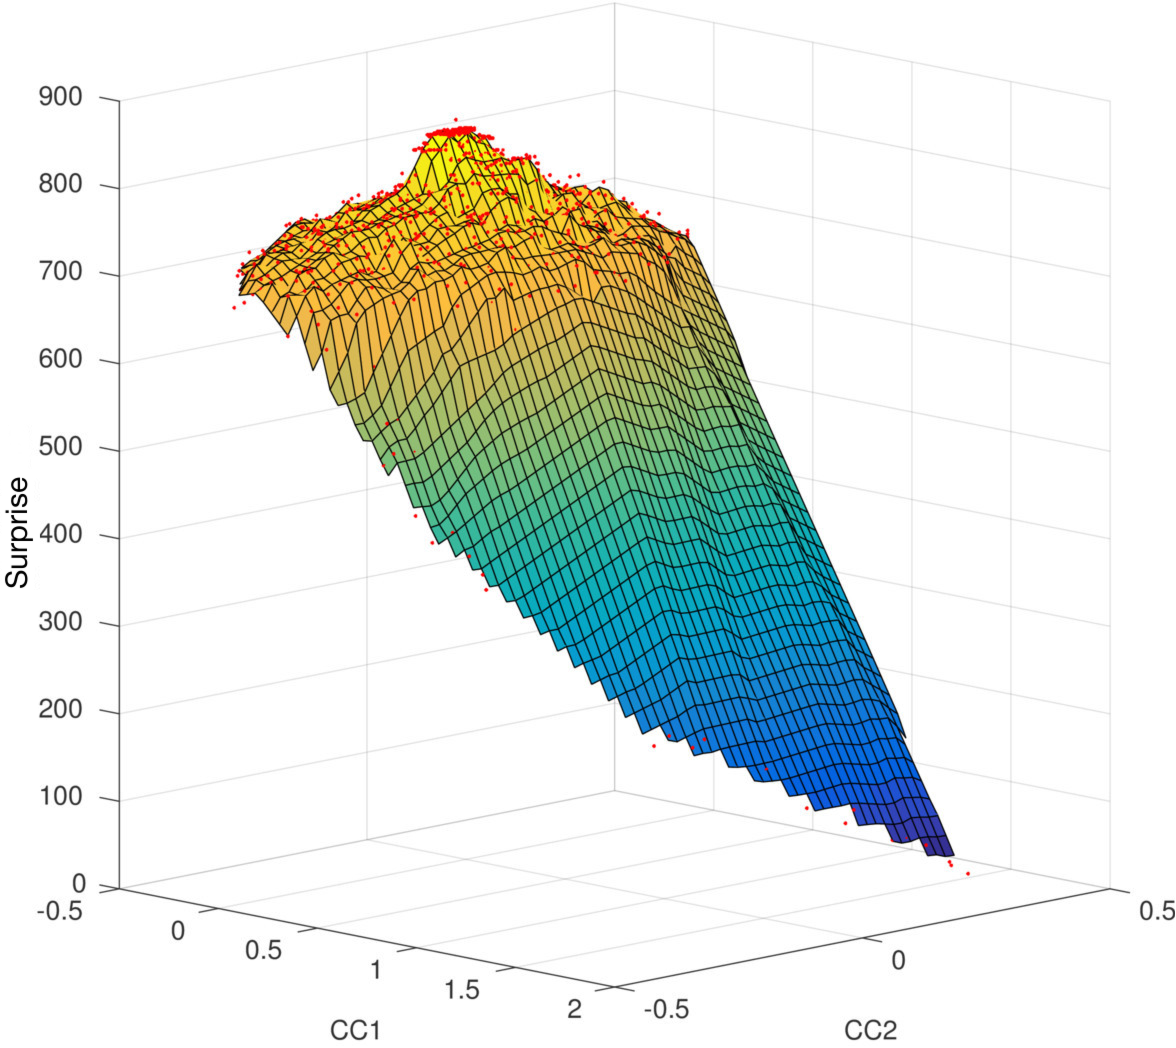
\includegraphics[height=0.4\textwidth]{images/degeneracy_surprise_n6_c30.png}
\caption{Degeneracy of Surprise landscape in a small (left) and large (right) ring of cliques graph. No plateaus exist, indicating the uniqueness of the global maximum that emerges from the other local optima.}
\label{fig:degeneracy_surprise}
\end{figure}

%%%%%%%%%%%%%%%%%%%%%%%%%%%%%%%%%%%%%%%%%%%%%%%%%%%%%%%%%%%%
%%%%%%%%%%%% MAXIMIZATION OF SURPRISE: FAGSO %%%%%%%%%%%%%%%
%%%%%%%%%%%%%%%%%%%%%%%%%%%%%%%%%%%%%%%%%%%%%%%%%%%%%%%%%%%%
\section{Maximization of Surprise: FAGSO}\label{sec:max_surprise_fagso}

Community detection is a NP-hard problem, and heuristics have to be developed for the optimization of quality functions for relatively large networks. In their original paper, Aldecoa et al.~\cite{aldecoa2011} applied metaheuristics, involving the evaluation of Surprise for partitions resulting from seven different community detection methods, each of those maximizing different quality functions.
Here, I describe direct maximization of Surprise by exploiting FAGSO~\cite{jiang2014} (Fast AGlomerative Surprise Optimization), an agglomerative optimization algorithm that builds on a variation of the Kruskal algorithm for minimum spanning tree~\cite{leiserson2001}.
The detailed pseudocode of this algorithm is reported in Algorithm~\ref{alg:fagso} and illustrated step by step on an example network in Figure~\ref{fig:fagso_working}.

The first step of FAGSO consists in ranking the edges in the graph in decreasing order by the Jaccard index of the neighbors of their two endpoints nodes.
An union-find data structure is used to hold the community structure throughout the computation.
At the beginning, each community consists only of one vertex.
Then, starting from the edge with the highest Jaccard index at the top of the list, the endpoints are attributed to the same community by disjoint-set union if this operation leads to a strictly better Surprise and if they do not belong already in the same community.
This step is repeated for all edges and the final community structure is returned in the disjoint-set.
FAGSO finds partitions with high Surprise and it is deterministic, unless two edges with the same Jaccard index are found. In this case, ties are broken at random. 
The implementation of FAGSO in \texttt{C++}, \texttt{Python} and \texttt{GNU Octave} is freely available at \url{https://github.com/carlonicolini/fagso}.
\begin{Algorithm}[htb!]
%%%% FAGSO %%%%
\begin{small}
\begin{codebox}
\Procname{$\proc{Fagso}(G)$}
\li $S\gets 0$ \Comment \emph{Initialize Surprise to $0$}
\li $D \gets \emptyset$ \Comment \emph{Initialize disjoint set forest}
\li \For each vertex $v$ in $V[G]$
\li \Do \proc{Make-Set}(v)
\End
\li $E' \gets \proc{Sort-Jaccard}(E)$ \Comment \emph{Sort edges in decreasing order by Jaccard index}
\li \For each edge$(u,v) \in E'$, \Comment \emph{Taken in decreasing order by Jaccard index}
\li \Do \If $\proc{Find-Set}(u) \neq \proc{Find-Set}(v)$
\li \Then \If $\proc{Surprise}(G,D \cup \{ (u,v)\} ) > S$
\li $D \gets D \cup  \{(u,v)\}$
\li $\proc{Union(u,v)}$ \Comment\emph{Merge the communities $u$ and $v$ belong}
\li $S=\proc{Surprise}(G,D)$ \Comment \emph{Update current Surprise}
\End
\End
\li
\Return $D$
\end{codebox}

%%%% MAKE-SET %%%%
\begin{codebox}
\Procname{$\proc{Make-Set}(x)$}
\li $p[x] \gets x$
\li $rank[x] \gets 0$
\end{codebox}
%%%% LINK %%%%
\begin{codebox}
\Procname{$\proc{Link}(x,y)$}
\li \If $rank[x]>rank[y]$
\li \Then $p[y]\gets x$
\li \Else $p[x]\gets y$
\li \If $rank[x] = rank[y]$
\li \Then $rank[y] \gets rank[y]+1$
\End
\End
\end{codebox}
%%%% UNION %%%%
\begin{codebox}
\Procname{$\proc{Union}(x,y)$}
\li \proc{Link}(\proc{Find-Set}$(x)$,\proc{Find-Set}$(y)$)
\end{codebox}
%%%% FIND-SET %%%%
\begin{codebox}
\Procname{$\proc{Find-Set}(x)$}
\li \If $x\neq p[x]$
\li \Then $p[x] \gets \proc{Find-Set}(p[x])$
\End
\li\Return $p[x]$
\end{codebox}
%%%% SURPRISE %%%%
\begin{codebox}
\Procname{$\proc{Surprise}(G,D)$}
\li $m_{\xi} \gets 0$ \Comment \emph{Number of intracluster edges}
\li $p_{\xi} \gets 0$ \Comment \emph{Number of intracluster pairs of vertices}
\li $m \gets |E[G]|$ \Comment \emph{Number of edges}
\li $p \gets \binom{\left| V[G]\right|}{2}$ \Comment \emph{Number of pairs of vertices}
\li \For each $g$ in $\proc{Connected-Components-Subgraphs}(D,G)$
\li \Do $m_{\xi} \gets m_{\xi} + \left|E[g]\right|$
\li $p_{\xi} \gets p_{\xi} + \binom{\left| V[g]\right|}{2}$
\End
\li \Return $-\log_{10}\left( \sum \limits_{i=m_\zeta}^m \dfrac{\binom{p_\xi}{i}\binom{p-p_{\xi}}{m-i}}{\binom{p}{m}} \right)$
\end{codebox}
%%%% MST PRIM %%%%
% \begin{codebox}
% \Procname{\proc{MST-Prim}$(G,w,r)$}
% \li \For each $u \in V[G]$
% \li \Do $key[u]\gets \infty$
% \li $\pi[u] \gets $ NIL \End
% \li $key[r] \gets 0$
% \li $Q \gets V[G]$
% \li \While $Q \neq \emptyset$ 
% \li \Do $u\gets \proc{Extract-Min}(Q)$
% \li \For each $v \in Adj[u]$ 
% \li \Do \If $v\in Q$ and $w(u,v) < key[v]$
% \li \Then $\pi[v]\gets u$
% \li $key[v]\gets w(u,v)$
% \End
% \End
% \End
% \End
% \End
% \end{codebox}
\end{small}
\caption{Pseudocode of FAGSO, with description of the implementation of union-find data structure.}
\label{alg:fagso}
\end{Algorithm}
\begin{figure}[htb!]
\centering
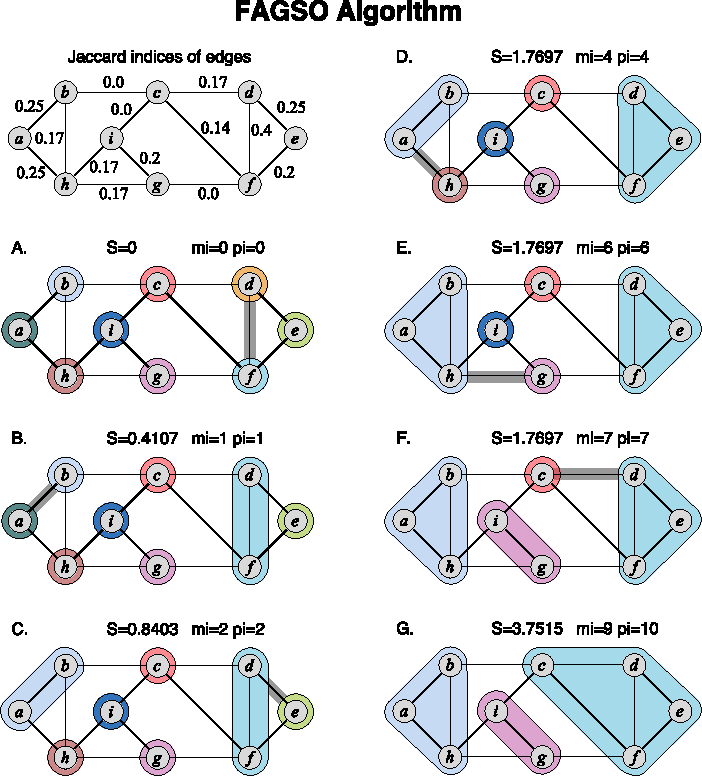
\includegraphics[width=0.8\textwidth]{images/fagso.pdf}
\caption{FAGSO algorithm steps illustrated. Firstly, Jaccard indices are computed. In box A., every node is associated to a separate community and FAGSO evaluates whether to merge nodes $d$ and $f$ in the same community as the edge they form has the highest Jaccard index. Since this merge results in an increased value of Surprise, $d$ and $f$ are merged in box B. then FAGSO proceeds to evaluate the merges of nodes $a$ and $b$ as their Jaccard index is the second greatest. FAGSO merges the two nodes in a second community and proceeds updating the Surprise value and analyzing the subsequent merges in boxes D to F, until no moves are available and FAGSO terminates with the community structure in box G.}
\label{fig:fagso_working}
\end{figure}

%%%%%%%%%%%%%%%%%%%%%%%%%%%%%%%%%%%%%%%%%%%%%%%%%%%%%%%%%%%%%%%%%%%%%%%%%%%%%%%%%%%%%%%%%%%%%%%%%%%%%
%%%%%%%%%%%%%% SURPRISE OPTIMIZATION ON FUNCTIONAL CONNECTIVITY NETWORKS %%%%%%%%%%%%%%%%%%%%%%%%%%%%
%%%%%%%%%%%%%%%%%%%%%%%%%%%%%%%%%%%%%%%%%%%%%%%%%%%%%%%%%%%%%%%%%%%%%%%%%%%%%%%%%%%%%%%%%%%%%%%%%%%%%
\section{Surprise optimization on functional connectivity networks}
\label{sec:surprise_optimization_fc_networks}
We assessed the performance of Surprise maximization by means of FAGSO in the detection of the community structure of two benchmark brain networks. All coordinate data and functional metadata were taken from the BrainMap database~\cite{fox2002,laird2005}, processed by Crossley et al.~\cite{crossley2013a} and made available to the scientific community as reference networks through the public Brain Connectivity Toolbox~\cite{rubinov2010}. I used BrainNetViewer as a tool for the visualization of the communities on brain templates~\cite{xia2013}.

%%%%%%%%%%%%%%%%%%%%%%%%%%%%%%%%%%%%%%%%%%%%%%%%%%%%%%%%%%%%%%%%%%
%%%%%%%%%%%%%% HUMAN RESTING STATE DATASET %%%%%%%%%%%%%%%%%%%%%%%
%%%%%%%%%%%%%%%%%%%%%%%%%%%%%%%%%%%%%%%%%%%%%%%%%%%%%%%%%%%%%%%%%%
\subsection{Human resting state dataset}\label{sec:restingstatedataset}
The first network represents the coactivation of brain regions as obtained from a meta-analysis of 1641 task-related fMRI or PET studies~\cite{crossley2013a}.
Meta-analyses have been useful in estimating the frequency with which two brain regions are consistently activated across different tasks and are an indication of the behavior of the brain during activity.
Jaccard similarity, i.e. the number of studies activating both regions divided by the number of studies activating either one of them, was used as index to evaluate strength of the coactivation of 638 parcellated brain regions. More details on the construction of the network are available in~\cite{crossley2013a}.

The second network that I considered is a resting state functional connectivity network obtained from correlations between time series of fMRI signals, from a group study of 27 healthy subjects. In short, fMRI data were acquired from 27 healthy volunteers at 3T. Gradient echo-planar imaging data were collected for 5 min with 2s TR and 13 and 31 ms echo-times. Thirty six interleaved 3mm slices with in-plane resolution of $3.5\times 3.5$ mm were acquired. 
Time series were extracted from 638 brain regions defined by a template~\cite{crossley2013a}, corrected for motion and band-passed (0.01–0.1Hz).
Functional connectivity was defined in terms of pairwise Pearson correlations at a subject's level.
A group-level functional connectivity matrix was calculated by averaging individuals' matrices after Fisher-transform\footnote{A mathematical transformation needed to correctly compute averages of correlation coefficients. Fisher transformation of a correlation coefficient $-1 \leq r \leq 1$ is computed as $\tanh(r)$ and ranges from $-\infty$ to $+\infty$.}, and thresholded to retain 18625 edges, as described in Crossley et al.~\cite{crossley2013a}.
Ethical statements are present in the original references by the groups who performed the experiments. 
The resting state network was built using the same set of 638 regions and thresholded to have the same number of edges as in the coactivation study.
Both networks have been previously studied using Modularity-based algorithms and node-classification methods~\cite{crossley2013a}.

Due to its definition in terms of binomial coefficients, Surprise can be computed for integer values of its parameters.
We have therefore binarized the two adjacency matrices retaining an equal number of edges for both networks.
While the binarization process discards information contained in the edge weights, a judicious choice of threshold can ensure robust decomposition of the network~\cite{meunier2010,he2009}.
We have checked this statement by percolation analysis, a natural and non-arbitrary method to derive binary graphs from continuous adjacency matrices (see section~\ref{sec:percolation_analysis}).
Specifically, I have studied the size of the largest connected component of the coactivation and resting state networks removing iteratively the smallest weight edges.

This analysis, shown in Figure~\ref{fig:figure_8_percolation_analysis}, revealed the presence of percolation-like transitions, whereby the largest component of the network drops in jumps with increasing binarization threshold. For the coactivation and the resting state networks I found that the thresholds adopted by~\cite{crossley2013a} of 0.015576 and 0.600, respectively, are above the first jump in the size of the largest connected components and maintain network connectedness while ensuring that the networks are sufficiently sparse and possess the same number of edges. Hence, I adopted these thresholds for network's binarization. Analysis of the structures of networks obtained by a range of thresholds around these values showed stable solutions, with Normalized Mutual Information close between partitions close to 1, and a stable number of communities (Figures~\ref{fig:figure_9_rs_threshold_study} and \ref{fig:figure_10_rs_threshold_study}).

\begin{figure}[htb!]
\centering
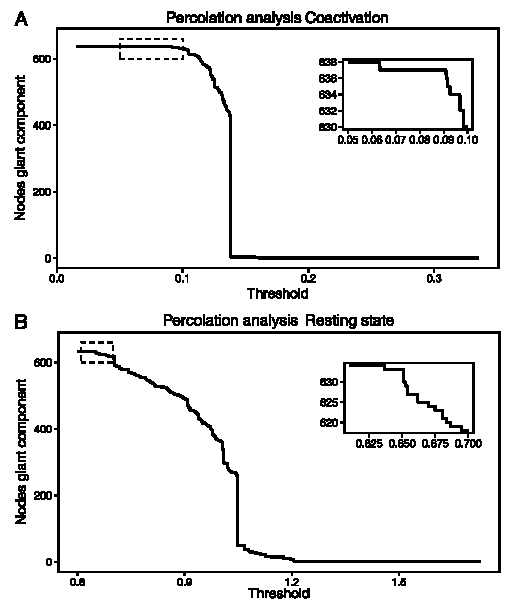
\includegraphics[width=0.7\linewidth]{images/figure_8_percolation_analysis_compressed.pdf}
\caption{Percolation analysis for the coactivation matrix (A) and resting state matrix (B).}
\label{fig:figure_8_percolation_analysis}
\end{figure}

\begin{figure}[htb!]
\centering
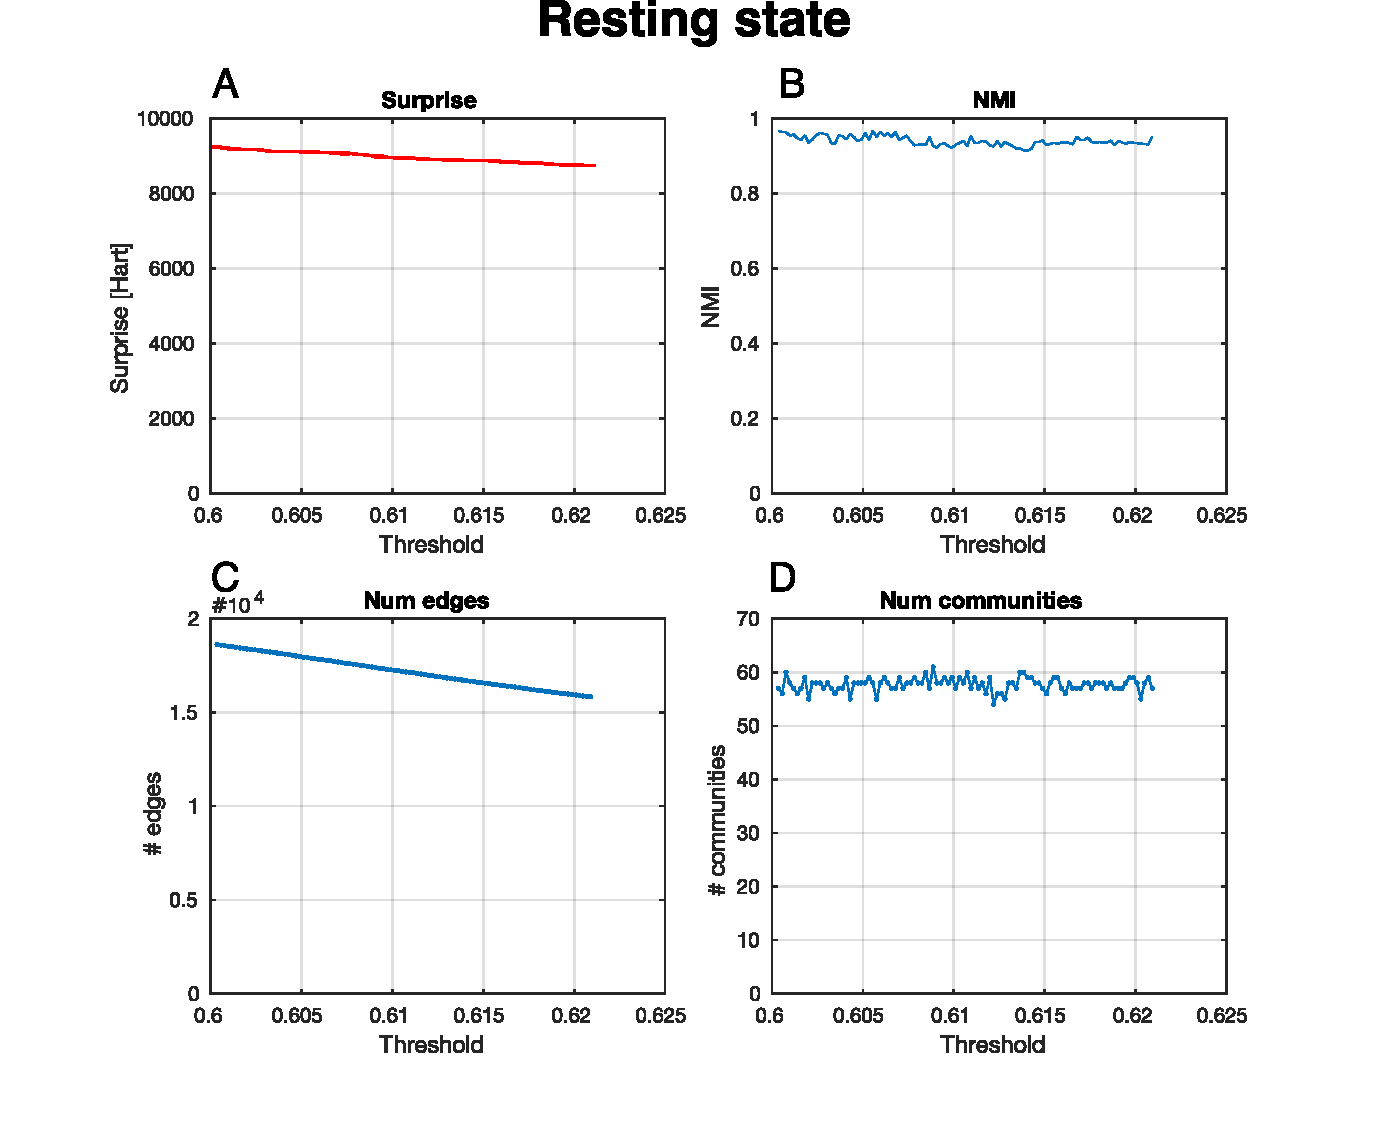
\includegraphics[width=0.7\linewidth]{images/resting_state_study_threshold.pdf}
\caption{Different Resting State networks were generated varying the binarization threshold in a range that changed the number of edges up to the 15th quantile of the edge weight distribution. This corresponds to threshold ranges of 0.015-0.03 for the co-activation network, and 0.60-0.62 for the resting state network. The resulting networks were partitioned by Surprise maximization. The value of Surprise, the Normalized Mutual Information between the resulting optimal partitions, the number of edges and the number of communities are reported in panel A, B, C and D, respectively.}
\label{fig:figure_9_rs_threshold_study}
\end{figure}

\begin{figure}[htb!]
\centering
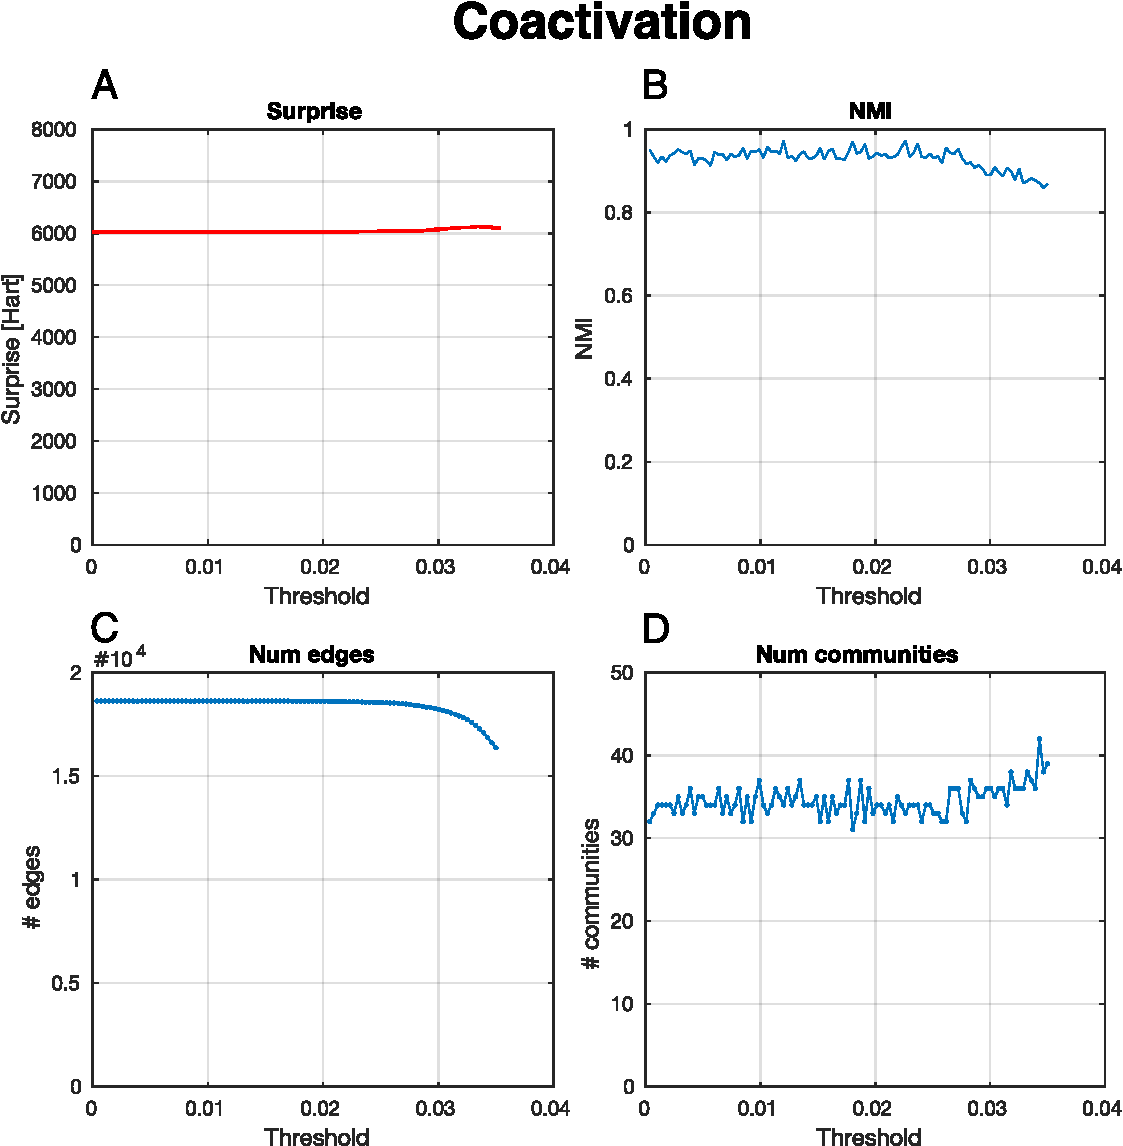
\includegraphics[width=0.7\linewidth]{images/coactivation_study_threshold.pdf}
\caption{Different coactivation networks were generated varying the binarization threshold in a range that changed the number of edges up to the 15th quantile of the edge weight distribution. This corresponds to threshold ranges of 0.015-0.03 for the co-activation network, and 0.60-62 for the resting state network. The resulting networks were partitioned by Surprise maximization. The value of Surprise, the Normalized Mutual Information between the resulting optimal partitions, the number of edges and the number of communities are reported in panel A, B, C and D, respectively.}
\label{fig:figure_10_rs_threshold_study}
\end{figure}

%%%%%%%%%%%%%%%%%%%%%%%%%%%%%%%%%%%%%%%%%%%%%%%%%%%%%%%%%%%%%%%%%%
%%%%%%%%%%%%%% COMMUNITY DETECTION RESULTS BY FAGSO %%%%%%%%%%%%%%%%%%%%%%%%%%%%%
%%%%%%%%%%%%%%%%%%%%%%%%%%%%%%%%%%%%%%%%%%%%%%%%%%%%%%%%%%%%%%%%%%
\subsection{Community detection results by FAGSO}
Figure \ref{fig:figure_3_communities_rs_coact_mod_surp} shows a direct comparison of the partitions obtained by Modularity and by Surprise maximization for the coactivation and resting state networks. The four panels display the adjacency matrices of the two networks, with their vertices rearranged by their module membership.

\begin{figure}[htb!]
\centering
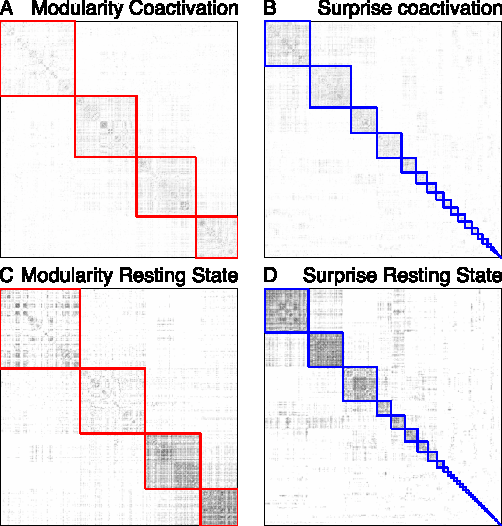
\includegraphics[width=1\linewidth]{images/figure_3_communities_rs_coact_mod_surp.pdf}
\caption{Modular structure of the coactivation and resting state networks under Modularity and Surprise maximization. The node indexes have been reordered by membership to highlight the modules, which are demarcated by a red line, for Modularity, or a blue line, for Surprise. Modularity maximization identifies only four, large modules, consistent with previous analysis of these data-sets. Surprise reveals a much finer and complex modular structure.}
\label{fig:figure_3_communities_rs_coact_mod_surp}
\end{figure}

By Newman’s decomposition, the resting state and coactivation brain networks present a modular structure with four large modules that have been anatomically labeled as occipital, central, frontoparietal and Default Mode networks~\cite{crossley2013a} (demarcated by a red line in Figure \ref{fig:figure_3_communities_rs_coact_mod_surp}). These partitions are highly similar (Rand Index 0.78), despite the different neurofunctional bases of the two networks~\cite{smith2009} and comprise modules that are relatively uniform in terms of number of nodes and number of edges within each module.

The partitions obtained by Surprise maximization for the two networks are shown in Figure \ref{fig:figure_3_communities_rs_coact_mod_surp}B, \ref{fig:figure_3_communities_rs_coact_mod_surp}D. Surprise found 51 communities, $\hat{S}=8969.24$, for the resting state network, and 28 communities, $\hat{S}=5725.65$ for the coactivation network.
These modules are delimited by blue lines that show the wide distribution in size of the components, ranging from communities with 119 nodes and 4586 edges down to singletons.
The size distributions of the modules are different for the two networks, with a more rapid drop and a fatter tail in the coactivation network compared with the resting state network.

The complete list of communities, with anatomical labels and stereotaxic coordinates for all nodes~\cite{laird2010,lancaster2007,tzourio2002}, as well as the density and number of nodes of each community found by Modularity and Surprise optimization, are reported in tabular form in the appendix (Tables~\ref{tab:densities_tables_mod_coact},~\ref{tab:densities_tables_modularity_rs},~\ref{tab:densities_tables_surprise_coact},~\ref{tab:densities_tables_surprise_rs}).

Analysis by Surprise suggests that the modular structure of resting state functional connectivity brain networks comprises modules of very different sizes, in sharp contrast with previous studies that have used resolution-limited functions like Newman's Modularity (see~\cite{meunier2010} for a review).
To emphasize this point, I have also partitioned the coactivation and resting state networks using Infomap~\cite{rosvall2008} and a multiscale version of Modularity with an adjustable resolution parameter~\cite{reichardt2006} provided by the Brain Connectivity Toolbox~\cite{rubinov2010}.
Interestingly, increasing the resolution parameter results in a larger number of smaller communities that are however characterized by a relatively homogeneous size distribution, a result of the intrinsic scale built into these methods (Figure~\ref{fig:figure_11_gamma_1_75_rs_coact}).
Additionally, I have made a quantitative comparison between the partitions obtained by Surprise, Infomap and the Reichardt and Bornholdt's method~\cite{reichardt2006} by calculating the Normalized Mutual Information between the resulting community structures (Tables~\ref{tab:coact_nmi_fagso}~\ref{tab:rs_nmi_fagso}). Despite the fact that these methods retrieve a few more modules that Newman's Modularity, they fail to capture the heterogeneous distribution of clusters revealed by Surprise. 

In order to assess the significance in neurofunctional terms of the finer partitions obtained by Surprise, I show the node distribution as an overlay of the MNI brain atlas template for the 10 largest modules of the resting state network in Figure \ref{fig:figure_4_resting_state_communities}. The communities highlighted by Surprise show a correspondence with some well-known functional networks previously identified by multivariate analysis (e.g. Independent Component Analysis) of functional MRI data~\cite{raichle2001,salvador2005,damoiseaux2006,deluca2006}, and with well-defined, segregated anatomical or functional districts.

\begin{figure}[htb!]
\centering
\includegraphics[width=1\linewidth]{images/figure_4_resting_state_communities.pdf}
\caption{The ten largest modules found by Surprise in the resting state network overlaid on an MRI brain template. The module indexes are ordered by decreasing size. The modules are named after corresponding functional networks previously identified by multivariate analysis of resting state fMRI data.}
\label{fig:figure_4_resting_state_communities}
\end{figure}

\begin{figure}[htb!]
\centering
\includegraphics[width=1\linewidth]{images/figure_5_communities_comparison.pdf}
\caption{Comparison of selected modules in the partition obtained by Surprise in the resting state and coactivation networks. The indexes are inversely ranked according to the size of the modules in their respective networks.}
\label{fig:figure_5_communities_comparison}
\end{figure}

\begin{figure}[htb!]
\centering
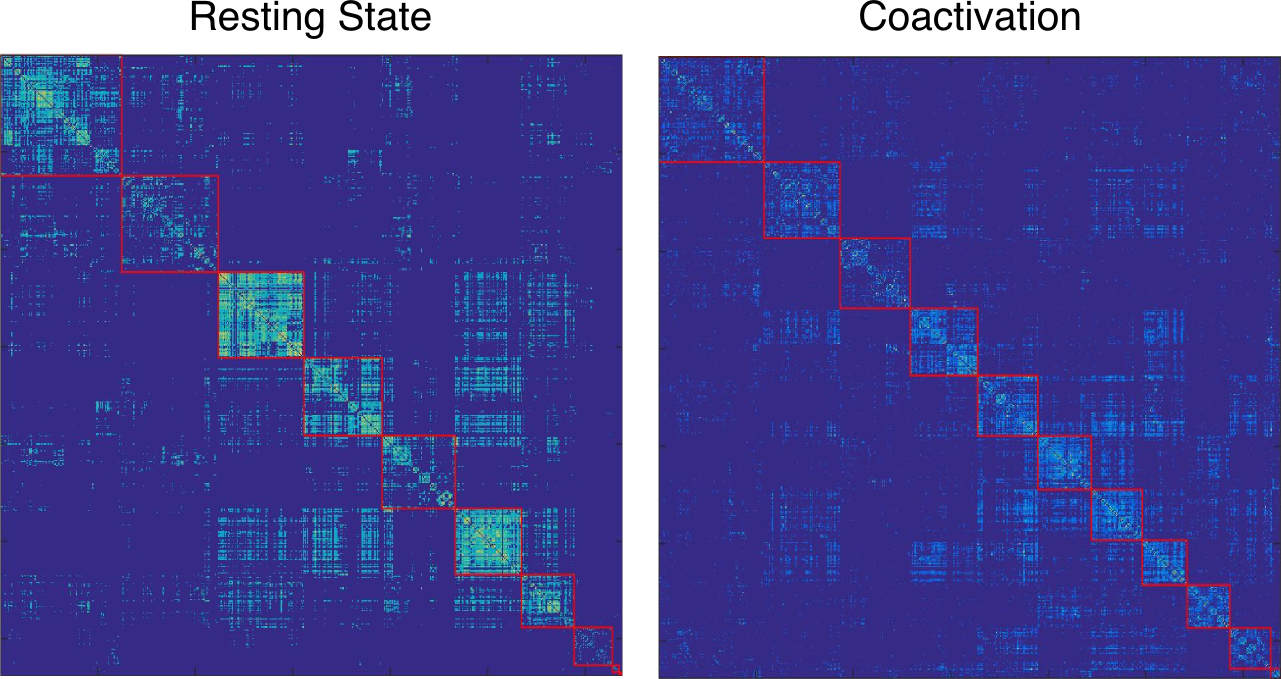
\includegraphics[width=1\linewidth]{images/coact_rs_gamma_1_75.png}
\caption{Partitions obtained with multiresolution Modularity (Reichardt and Bornholdt method) for a value of the resolution parameter $\gamma=1.75$ for the coactivation and resting state networks. Increasing the resolution parameter improves detection of smaller modules, but breaks up larger ones, thus resulting in relatively homogeneous size distributions.}
\label{fig:figure_11_gamma_1_75_rs_coact}
\end{figure}

\begin{table}
\centering
\begin{tabular}{ccccc}
& & \textbf{Coactivation} & \\
\hline 
\textbf{NMI} &Modularity & Surprise & Infomap & RB $\gamma=1.75$ \\
\hline
Modularity 			& \textbf{1.00} & 0.61 & 0.56 & 0.61 \\
Surprise 			& 0.61 & \textbf{1.00} & 0.54 & 0.62 \\
Infomap 			& 0.56 & 0.54 & \textbf{1.00} & 0.59 \\
RB $\gamma=1.75$ 	& 0.59 & 0.61 & 0.59 & \textbf{1.00} \\ \hline 
\end{tabular}
\caption{Normalized Mutual Information between partitions of the coactivation network with Newman's Modularity, Infomap, Reichardt and Bornholdt and Surprise.
We used the Fagso algorithm for Surprise maximization, the \texttt{igraph} implementation of Infomap, the Brain Connectivity Toolbox implementation for RB (\texttt{community\_louvain.m} function) and \texttt{modularity\_und.m} for Modularity.
For each method the best solution over 100 repetitions was used to calculate NMI.}
\end{table}

\begin{table}
\centering
\begin{tabular}{ccccc}
& & \textbf{Resting State} & \\
\hline 
\textbf{NMI} &Modularity & Surprise & Infomap & RB $\gamma=1.75$ \\
\hline
Modularity & \textbf{1.00} & 0.52 &  0.70 & 0.66 \\
Surprise & 0.52 & \textbf{1.00} & 0.53 & 0.58 \\
Infomap & 0.70 & 0.53 & \textbf{1.00} & 0.68 \\
RB $\gamma=1.75$ & 0.66 & 0.58 & 0.68 & \textbf{1.00} \\ \hline 
\end{tabular}
\caption{Normalized Mutual Information between partitions of the Resting state network with Newman's Modularity, Infomap, Reichardt and Bornholdt and Surprise.
We used the Fagso algorithm for Surprise maximization, the \texttt{igraph} implementation of Infomap, the Brain Connectivity Toolbox implementation for RB (\texttt{community\_louvain.m} function) and \texttt{modularity\_und.m} for Modularity.
For each method the best solution over 100 repetitions was used to calculate NMI.}
\end{table}

\begin{table}
\centering
\begin{tabular}{lccccc}
& &\textbf{Coactivation}	&	&	&\\
\hline
&\textbf{NMI}&	Surprise &	Infomap&	RB $\gamma=1.75$\\ \hline
\textbf{RS} &Surprise& 0.59&0.40&0.52\\
	&Infomap & 0.54&0.44&0.51\\
	&RB $\gamma=1.75$ &0.59&0.41&0.53\\ \hline 
\end{tabular}
\caption{Normalized Mutual Information between Resting State (RS) and Coactivation (Coact) partitions. Infomap and RB methods are repeated 100 times and partitions with the highest quality are used. NMIs are approximated to second significant digit.}
\end{table}

The largest communities of the resting state network correspond to the primary sensorimotor cortex~\cite{biswal1995}, primary visual and extra-striate visual network, fronto-parietal lateralized networks~\cite{smith2009} as well as the so-called default mode network (DMN)~\cite{raichle2001,fransson2006}.
The attentional frontoparietal networks (FPAN)~\cite{beckmann2005} were detected as two separate, lateralized subnetworks, in agreement with~\cite{deluca2006} although other studies have identified a single, bilateral FPAN~\cite{markett2014}.

Smaller networks, like the executive control and auditory networks~\cite{salvador2005,vandenheuvel2010} were also resolved by Surprise, as well as subcortical structures, like the hippocampal and thalamic formations~\cite{roy2009,chen2013}. Interestingly, the thalamic nuclei appear as one tight community, despite the fact that they are structurally unconnected, in keeping with the idea that functional connectivity does not necessarily require the presence of strong structural links.

The more accurate partition afforded by Surprise may enable identification of differences in the modular structures of networks that cannot be appreciated with a resolution limited method. By way of example, I have compared the partitions of the resting state and coactivation networks (Figure \ref{fig:figure_5_communities_comparison}). Indeed, these networks are of a different nature, the former representing intrasubject baseline fluctuations in the brain's resting state, and the latter the responses to a variety of different tasks across subjects. However, Newman's Modularity finds similar partitions for these two networks, with 4 large modules each.

Conversely, under Surprise maximization, the partition of the resting state network shows many more small communities comprising less than 5 nodes (32 in total) compared with the coactivation one (only 11). Moreover, certain communities of the resting state network appeared to be split into smaller modules in the coactivation matrix. 
By way of example, the cuneus and the lingual and pericalcarine gyri were part of the occipital visual module in the resting state, but not in the coactivation network, where they formed a separate community (first row of Figure \ref{fig:figure_5_communities_comparison}).
Similarly, the precuneus and medial parts of the postcentral gyrus were identified as an independent community in the coactivation network, while they were part of the broad somatosensory network in the resting state connectivity graph~\cite{rubinov2011} (second row of Figure \ref{fig:figure_5_communities_comparison}).
Interestingly, the Broca area, indicated as Module 11 in Figure \ref{fig:figure_5_communities_comparison}, was separated from the auditory network in the coactivation network, and identified as a small, but anatomically and functionally distinct, community.
Conversely, other communities were split in the resting state but not in the coactivation network. The executive and attentional control networks were merged into a large community in the coactivation network, while they were separated under resting state conditions, including a subdivision of the left and right fronto-parietal networks (third row of Figure \ref{fig:figure_5_communities_comparison}).

While the resting state and coactivation networks appeared to possess virtually identical modular structures under Newman's analysis, they showed functionally and anatomically relevant differences when analyzed by Surprise maximization, with a Normalized Mutual Information between the partitions of the two networks of 0.5922. Indeed, Modularity tends to assign small communities to larger structures even when they correspond to tightly-knit modules, thus concealing differences in the graphs' modular structures that involve aggregation or disaggregation of smaller clusters. It is conceivable that the detrimental effects arising from the resolution limit may have affected previous studies comparing different populations~\cite{meunier2010}.
Surprise may offer a sharper tool to detect alterations of brain connectivity induced, for example, by psychiatric or neurological conditions, thus enabling the exploration of novel markers of brain disease.

%%%%%%%%%%%%%%%%%%%%%%%%%%%%%%%%%%%%%%%%%%%%%%%%%%%%%%%%%%%%%%%%%%%%%%%%%%%%%%
%%%%%%%%%%%%%%%%%%%%%%% HUBS CLASSIFICATION %%%%%%%%%%%%%%%%%%%%%%%%%%%%%%%%%%
%%%%%%%%%%%%%%%%%%%%%%%%%%%%%%%%%%%%%%%%%%%%%%%%%%%%%%%%%%%%%%%%%%%%%%%%%%%%%%
\subsection{Hubs classification}
Besides the exploration of functional and anatomical segregation, understanding the modular structure of brain networks is critical for the interpretation and classification of the roles played by the nodes within the network structure~\cite{sporns2007}. Highly connected nodes, or hub nodes, are particularly important for their topological centrality, and function as integrators. Hubs that primarily connect to nodes within the same module are dubbed ``provincial hubs'', and nodes that connect different modules are referred to as ``connector hubs''. The former are thought to be responsible for the formation and stability of the modules, while the latter ensure integration of the activity of the different modules. Obviously, interpretation of the hub's role relies on the correct identification of the optimal network partition, and may be strongly affected by the resolution limit.

Here, I have performed a hub's role analysis for the resting state and coactivation networks under Modularity and Surprise maximization.
To this end, I have adopted Guimera' and Amaral classification scheme~\cite{guimera2005}, whereby nodes are classified by their within-community degree $z$ (a measure of how well-connected a node is to other nodes in the same community) and their participation coefficient $P$, a parameter that is $0$ for nodes with purely intra-module connections and $1$ for nodes whose links project primarily to other modules. 

Figures \ref{fig:figure_6_ga_rs_coact}A and \ref{fig:figure_6_ga_rs_coact}B show the different positioning of high-degree nodes in the Guimera' and Amaral plot for the coactivation and resting state networks partitioned using Newman’s approach and Surprise maximization. In this scheme, provincial hubs are high-degree nodes that score high $z$ and low $P$ values (\emph{R5} region); conversely, connector hubs are characterized by larger $P$ values (regions on the right-hand side of the plot).

\begin{figure}[ht!]
\centering
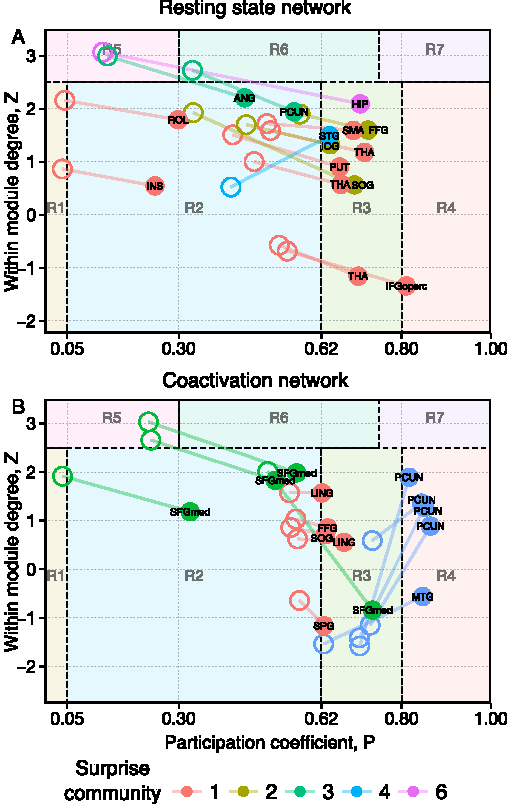
\includegraphics[width=0.5\linewidth]{images/figure_6_ga_rs_coact.pdf}
\caption{Classification of representative nodes according to their intra- and intermodule connections for the resting state (A) and coactivation (B) networks. Empty circles and full circles indicate the position of each node in the Guimera' and Amaral’s plot after partition by Modularity or Surprise, respectively. An overall increase in the participation coefficient, a measure of the intermodule connectivity, is observed for the Surprise partition relative to the Modularity partition. To avoid cluttering of the graph, I only reported those nodes with a degree higher than the average within a Standard Deviation, and whose classification is different in the two partitions. The abbreviations of the brain regions corresponding to the nodes are reported in the appendix, Table~\ref{tab:abbreviations}.}
\label{fig:figure_6_ga_rs_coact}
\end{figure}

A finer partition in smaller communities may be expected to determine an overall increase in participation coefficient and decrease in within-community degree. However, the heterogeneous partitions obtained by Surprise maximization resulted in non-trivial changes in the Guimera' and Amaral classification. By way of example, I discuss in greater detail two regions whose roles are very different in the two partitions, to highlight the effects of the resolution limit.

Nodes that belong in the hippocampal formation show a large within-module coefficient, and appear as provincial hubs (region R5 of Figure \ref{fig:figure_6_ga_rs_coact}) under Modularity optimization. However, their participation coefficient increases 6-fold in the partition by Surprise, which reveals a role as connectors for these nodes, with widespread projections to many other modules across the brain, including the module 3, 6, 8, 5, 2, corresponding to the DMN, the amygdala and parahippocampal formation, the temporal inferior gyrus, the cuneus and lingual gyrus, and the visual cortex, respectively.
This finding is in agreement with the idea that the hippocampus acts as ``network convergence zone'', as it receives polysensory input from distributed association areas in the neocortex~\cite{misic2014}.

Interestingly, the right shift in the Guimera-Amaral plot is less pronounced for the nodes in the posterior part of the hippocampus (Figure \ref{fig:figure_7_ga_coact_hippocampus}). A differential classification of the anterior and posterior hippocampus is consistent with the hypothesis of a functional differentiation of this structure~\cite{moser1998}, with the posterior hippocampus mostly involved in memory and cognition, and the anterior hippocampus playing a role in the processing of stress, emotion and affect~\cite{fanselow2010}. Moreover, studies in animal models have shown differential organization of the efferent connections of the hippocampal formation~\cite{swanson1977}, consistent with different functions for the anterior and posterior hippocampus.

\begin{figure}[htb!]
\centering
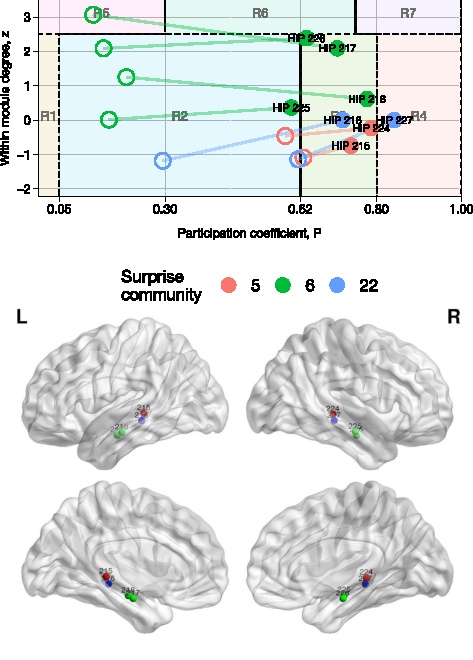
\includegraphics[width=0.5\linewidth]{images/figure_7_hippocampus.pdf}
\caption{Top panel: classification of all the hippocampal nodes according to the Guimera' and Amaral's scheme for the coactivation network. Empty circles and full circles indicate the position of each node after partition by Modularity or Surprise, respectively. Bottom panel: anatomical positions of the nodes in the hippocampal formation, colored by Surprise community membership. The increase in participation coefficient upon partition by Surprise is more pronounced for nodes in the anterior part of hippocampus, with an antero-posterior gradient.}
\label{fig:figure_7_ga_coact_hippocampus}
\end{figure}

Similar rightward shifts for nodes and hubs were observed in the resting state network, and reported in Figure \ref{fig:figure_6_ga_rs_coact}.
However, increases in participation coefficients are by no means the only differences in the classification of nodes obtained by Surprise maximization. A prominent example is the precuneus (PC) (Figure \ref{fig:figure_6_ga_rs_coact}B, blue dots) that shows a high participation coefficient in both partitions by Modularity and Surprise, but a much higher within-module degree under Surprise maximization.

Indeed, the nodes comprised in the precuneus intrinsically possess high inter-cluster connectivity, but are distributed among the four modules found by Modularity. In the partition by Surprise they are grouped together, and this precuneal module as a whole plays a connector's role integrating different communities (Figure \ref{fig:figure_8_ga_rs_precuneus}), a hypothesis that is consistent with the precuneus supporting a wide spectrum of highly integrated tasks, from visuo-spatial imagery to episodic memory retrieval and self-processing operations~\cite{cavanna2006}.

In summary, partition by Surprise maximization results in very different distributions of participation coefficients and within-module degree compared to Modularity. These differences are not uniform across nodes, and arise from the limited ability of Modularity to identify small modules. Finer partition by Surprise reveals very different roles for some key brain areas, and suggests that a systematic reanalysis of the topological roles of brain nodes and hubs may be in order.

\begin{figure}[htb!]
\centering
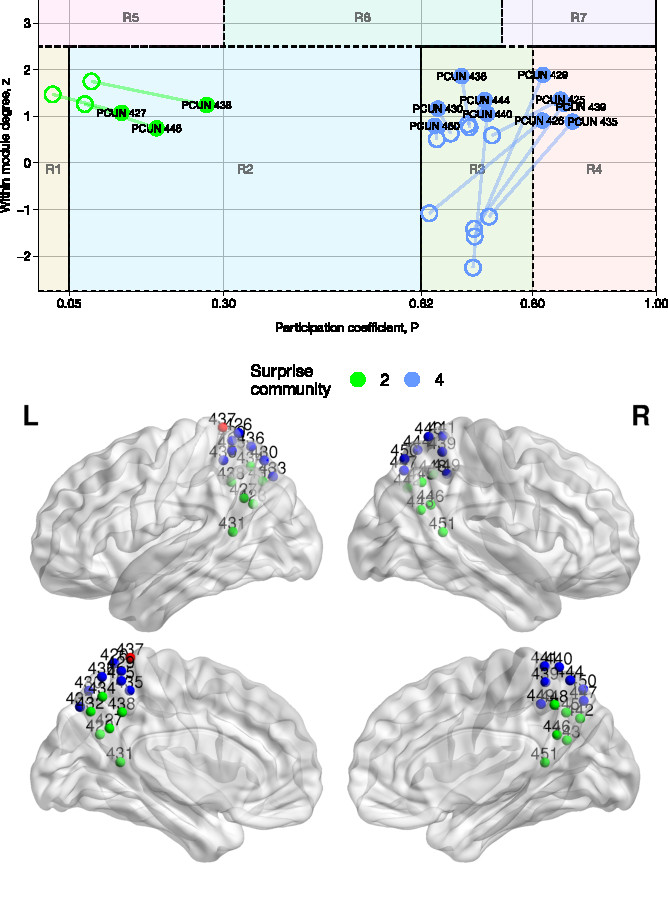
\includegraphics[width=0.5\linewidth]{images/figure_8_precuneus.pdf}
\caption{Top panel: classification of the precuneal nodes according to the Guimera' and Amaral's scheme for the resting state network. Empty circles and full circles indicate the position of each node after partition by Modularity or Surprise, respectively. Bottom panel: anatomical positions of the nodes in the precuneus, colored by Surprise community membership. The nodes in the dorsal part of the precuneus exhibit a sharp increase in within-module degree.}
\label{fig:figure_8_ga_rs_precuneus}
\end{figure}


%%%%%%%%%%%%%%%%%%%%%%%%%%%%%%%%%%%%%%%%%%%%%%%%%%%%%%%%%%%%%%%%%%%%%%%%
%%%%%%%%%%%%%% LIMITATIONS OF BINARY SURPRISE %%%%%%%%%%%%%%%%%%%%%%%%%%
%%%%%%%%%%%%%%%%%%%%%%%%%%%%%%%%%%%%%%%%%%%%%%%%%%%%%%%%%%%%%%%%%%%%%%%%
\section{Limitations of binary Surprise}
A potential limitation of Surprise is related to its definition in terms of discrete probability distributions. This makes Surprise suited for the study of binarized networks. While the topological backbones of the networks I have investigated appear quite robust against removal of lowest-weight edges and binarization, as shown by our percolation and stability analyses (Figures~\ref{fig:figure_8_percolation_analysis},~\ref{fig:figure_9_rs_threshold_study},~\ref{fig:figure_10_rs_threshold_study}), the application of its weighted counterpart, Asymptotical Surprise, will help overcome the need of binarization.

The superior resolution afforded by Surprise may make it more vulnerable than other methods to noise and experimental errors. Indeed, occasional misassignment of nodes due to noise-induced changes in edge distribution are likely to affect small modules, comprising only a few nodes, more than large ones. Hence, experimental uncertainty also limits resolution, and a resolution-limit-free method would not necessarily improve the quality of the partition in a scenario dominated by noise. 

To ascertain whether this is the case for the co-activation and resting state networks investigated here, I have simulated the effects of experimental errors by injecting noise into the distributions of weights prior to the binarization procedure, thus introducing variability in the connectivity structure of the resulting binary networks.
We set levels of noise sufficient to perturb up to 10\% of the edges of the final binary network. Using this procedure, for each level of noise I generated ten different graphs, and applied the Surprise Maximization algorithm to each of them. 

The ten different graphs were generated by adding noise to the off-diagonal elements of the adjacency matrix prior to the binarization procedure. The amplitude of noise was chosen to randomly perturb 10\% of the edges after binarization. Surprise maximization was applied to the resulting graphs. In the left panel of Figure~\ref{fig:figure_9_nmi}, I reported the Normalized Mutual Information (NMI) between the optimal partitions of each of the ten perturbed networks and that of the original resting state network.
The number of communities retrieved by FAGSO in each of the perturbed networks is reported in the right panel of Figure~\ref{fig:figure_9_nmi}. The graphs show that the partitions of the ``noisy'' graphs are consistent and similar to those of the unperturbed network, with NMI scores close to 1 and almost constant numbers of communities.
These results demonstrate that Surprise maximization can retrieve the network's community structure even in the presence of substantial noise in the data.
We found that the partitions of these graphs were highly consistent with those of the original networks (Figure~\ref{fig:figure_9_nmi}).

\begin{figure}[ht]
\centering
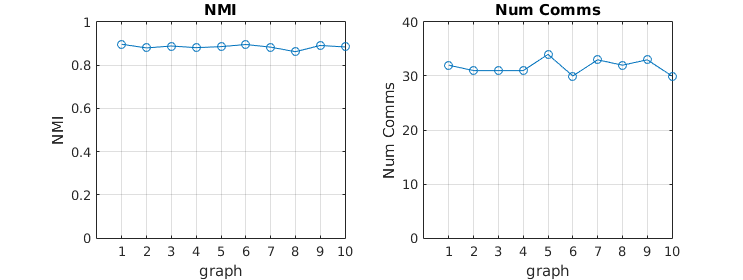
\includegraphics[width=1\linewidth]{images/figure_9_nmi.png}
\caption{Assessment of the effects of experimental error on the community structure of the resting state network.}
\label{fig:figure_9_nmi}
\end{figure}

We should also stress that there is no constraint in the FAGSO algorithm imposing inter-hemispherical symmetry of the partition.
Nevertheless, I observed homotopic correspondence in the community structure, and a close resemblance with established neurofunctional circuits as in Figure~\ref{fig:figure_4_resting_state_communities} and~\ref{fig:figure_5_communities_comparison}. Taken together, simulations of the effects of noise and qualitative considerations on the neurofunctional significance of the modules identified by Surprise corroborate the idea that experimental error is not the predominant factor in the networks investigated.

A final and important point I should highlight is that Surprise maximization, in the implementation I have used here, does not allow for overlapping communities. Other methods have been applied to investigate this aspect in brain networks~\cite{palla2005,ahn2010}. However, a recent comparative analysis of graph partitioning algorithms on a variety of benchmark networks~\cite{lancichinetti2009} has shown that these methods are also prone to merging overlapping communities, with relatively modest performance in recovering heterogeneous cluster distributions planted in model networks.
Despite these potential limitations, the resolution-limit-free behavior of Surprise makes it an excellent tool to explore and to overcome the effects of the resolution limit in the modular structure of brain connectivity networks.


%%%%%%%%%%%%%%%%%%%%%%%%%%%%%%%%%%%%%%%%%%%%%
%%%%%%%%%%%%%% CONCLUSIONS %%%%%%%%%%%%%%%%%%
%%%%%%%%%%%%%%%%%%%%%%%%%%%%%%%%%%%%%%%%%%%%%
\section{Conclusions}
In conclusion, I have shown that Surprise, a recently proposed fitness function for graph partitioning, behaves like a resolution-limit-free function.
I have applied Surprise maximization to study the modular structures of two different brain networks.
Surprise maximization resulted in partitions comprising communities of widely distributed sizes, consistent with the idea that small and large modules coexist in brain networks.
Moreover, the finer partition afforded by Surprise made it possible to appreciate differences in the modular structures of diverse brain networks that were undetected by resolution limited methods like Newman's Modularity.
Finally, the use of Surprise revealed the deleterious effects of the resolution limit in the classification of nodal roles.
Altogether, these results indicate that the resolution limit may have substantially affected many of the analyses of brain connectivity networks reported in the literature, and call for a revisitation of some of the conclusions and models that have relied on Modularity maximization or similarly resolution-limited algorithms.
Surprise appears as a promising alternative method that appeals to the intuition that tightly-knit clusters of nodes represent legitimate structural
or functional modules independently of their size.

\chapter{Beyond the resolution limit in weighted networks}\label{chap:beyondresolutionlimitweightednetworks}
Brain networks are intrinsically weighted with weights reflecting a continuous distribution of connectivity strengths between different regions.
A fundamental limitation of Surprise lies in its definition in terms of discrete probability and binomial coefficients that make it applicable only to binary networks, i.e. graphs with edge values $1$ or $0$.
For this reason Surprise requires binarization of brain connectivity networks, a process that may discard potentially important information contained in the edge weights distribution. 
Moreover, different binarization procedures may lead to different network representations for the same connectivity dataset.
This represents a substantial drawback of the binary Surprise approach.

Hence, an extension of Surprise to weighted networks would be highly desirable, and would provide a new and important tool to study the modular organization of brain connectivity beyond the resolution limit.
The results obtained from binary Surprise optimization on real functional connectivity networks, encouraged me to extend the Surprise optimization approach to weighted networks.

Capitalizing on recent developments in the field of statistical physics of complex networks~\cite{traag2015}, here I show that Surprise can be extended to weighted networks. This recently introduced approach dubbed Asymptotical Surprise, provides a new and important tool to study the modular organization of brain connectivity beyond the resolution limit.
Furthermore, I'll present a new algorithm for the optimization of Asymptotical Surprise in the study of the modular structure of weighted networks.

% Since there is no ground-truth structure for brain functional connectivity networks, I have assessed the performance of this novel approach on synthetic networks with a planted modular structure, and compared it to some of the leading graph partitioning methods, namely Louvain method for Newman's Modularity (see section~\ref{sec:louvain_method}) and Infomap.
Importantly, I will demonstrate this new approach in networks derived from synthetic data that mimic different structures, levels of noise and variability, such as those observed in functional connectivity experimental data.
Indeed, improved resolution afforded by Asymptotical Surprise may imply increased vulnerability to spurious modules resulting from noisy correlations.
It is therefore important to assess the benefits of increased resolution against the limitations arising from intrinsic data variability. 

Finally, I'll apply Asymptotical Surprise to weighted functional connectivity networks from resting state fMRI data, revealing a heterogeneous, multiscale community structure.
I'll show that the finer modular subdivision of resting state functional connectivity networks obtained by Asymptotical Surprise leads to substantial differences in the identification of connector hubs compared to other community detection methods.

\section{Asymptotical Surprise}
In developing a quality function inspired to the principle of Surprise that works for weighted networks, it's convenient to consider the asymptotical expansion of the hypergeometric distribution. Hereafter I'll stick to the derivation obtained by Traag~\cite{traag2015}.
One can introduce $q=m_\zeta/m$ and $\left<q \right>=p_\zeta/p$ as the observed and expected fraction of intracluster edges. By only taking into account the dominant term of the sum in Eq.~\ref{eq:surprise} (the one with $i=m_\zeta$), after some manipulations one gets an approximate expression for the logarithmic Surprise\footnote{If not specified, starting from here we use natural base logarithms.}:
\begin{equation}\label{eq:surprise_dominant}
\log(S) \approx \log \left( \frac{\binom{\left<q\right> p}{m_\zeta} \binom{(1-\left<q\right>)p}{m(1-q)}}{\binom{p}{m}} \right)
\end{equation}
which corresponds to the probability of observing exactly $m_\zeta$ internal links, given the clustering $\zeta$.
As the denominator in Eq.\ref{eq:surprise_dominant} is independent of the partition, it can be discarded, and, thanks to the Stirling approximation of the binomial coefficients, which reads 
\begin{equation}
\log \binom{n}{k} \approx k \log \left( \frac{n}{k} \right)
\end{equation}
one can write the dominant term~\ref{eq:surprise_dominant} as:
\begin{equation}
\log(S) = - \log \left(\frac{m}{p}\right)^{-m} \left[ \left(\frac{\left< q\right>}{q}\right)^q \left(\frac{1-\left< q\right>}{1-q}\right)^{1-q} \right]^{m}
\end{equation}
The term $(m/p)^{-m}$ is independent of the partition so it can be discarded.
Hence, the asymptotic expansion of Surprise reads:
\begin{equation}
\log(S) = -m \left[ q \log \frac{\left<q\right>}{q} + (1-q)\log \frac{1-\left<q\right>}{1-q} \right]
\end{equation}
Interestingly, this last equation corresponds to the binary Kullback-Leibler divergence $m D_{KL}(q \| \left< q \right>)$, which is interpretable as the distance between the two probability distributions $q$ and $\left<q\right>$.
More precisely, as the information lost (in nats since we are using natural base logarithms) when one encodes the distribution $q$ with the distribution $\left< q\right>$.
Thus, in the limit of large networks, Surprise $\hat{S}$ can be approximated by a binomial distribution.
This observation led to definition of Asymptotical Surprise $\mathcal{S}_a$~\cite{traag2015}:
\begin{equation}\label{eq:asymptoticalsurprise}
\mathcal{S}_a = m D_{\textrm{KL}}\left( q \| \left< q \right> \right)
\end{equation}
where the binary Kullback-Leibler divergence~\cite{kullback1951} is $$D_{\textrm{KL}}(x\|| y) = x \log \left(\frac{x}{y} \right) + (1-x)\log \left (\frac{1-x}{1-y} \right).$$

In the framework of information theory~\cite{cover2006}, Asymptotical Surprise represents the Kullback-Leibler divergence between the observed and expected fraction of intra-cluster edges; it encodes the information lost when the prior distribution $\left <q \right >$ is used to approximate the posterior distribution $q$. Kullback-Leibler divergence is a quasi-distance on probability distributions as it is always non-negative, non-symmetric and zero only when $q=\left< q \right>$, exactly like binary Surprise.

Asymptotical Surprise has a simpler formulation than binary Surprise as there are no binomial coefficients to evaluate and it has been shown to be resolution-limit-free in the limit of large networks~\cite{traag2015}. As a side effect of its definition in terms of information-theoretic quantity, Asymptotical Surprise transparently allows the extension of Surprise to weighted networks, when the intracluster density now consider edge weights.
This powerful property made Asymptotical Surprise suited for community detection in weighted networks and in particular to brain functional connectivity networks, thus avoiding the need of binarization procedures prior to the community detection, as shown in~\cite{nicolini2017}.

Given its information-theoretic formulation, Asymptotical Surprise cleary features \emph{convexity}, a property that is more difficult to assess for binary Surprise. Optimization of convex functions is typically simpler due to some regularities featured by such functions and the availability of practical algorithms. Furthermore a convex function warranties a landscape with a global optimum and no degeneracy, a property that is extremely important for community detection.

Yet, numerical evalaution of Asymptotical Surprise is much faster than binary Surprise, furthermore it approximates very well Surprise already for networks with more than 50 nodes, as shown in Figure~\ref{fig:asymptotical_surprise_comparison}.

\begin{figure}[!htb]
\centering
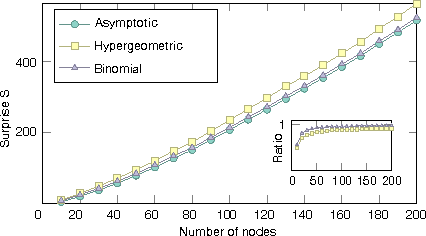
\includegraphics[width=1\textwidth]{images/asymptotical_surprise_comparison.pdf}
\caption{Approximation of binary Surprise with a binomial formulation and the Asymptotical formulation based on the Kullback-Leibler divergence. In the inset, the approximation ratio of binomial and Asymptotical Surprise to hypergeometric Surprise tends to 1 for graphs larger than 50 nodes. Adapted from~\cite{traag2015}.}
\label{fig:asymptotical_surprise_comparison}
\end{figure}

%%%%%%%%%%%%%%%%%%%%%%%%%%%%%%%%%%%%%%%%%%%%%%%%%%%%%%%%%%%
%%%%%%%%%%%%%%%%%%%%%%%%%% PACO %%%%%%%%%%%%%%%%%%%%%%%%%%%
%%%%%%%%%%%%%%%%%%%%%%%%%%%%%%%%%%%%%%%%%%%%%%%%%%%%%%%%%%%
\section{Maximization of Asymptotical Surprise: PACO}
Finding the optimal partition of a graph is an NP-hard problem~\cite{fortunato2010} and practical implementations of community detection rely on heuristic approaches that enable finding nearly-optimal solutions in a reasonable computation time.

Here I introduce a powerful and general method for the optimization of Asymptotical Surprise dubbed PACO (PArtitioning Cost Optimization).
PACO is a non-deterministic agglomerative algorithm based on FAGSO (described in chapter~\ref{sec:max_surprise_fagso}) and, like the Louvain method, has an element of randomness that enables a more efficient exploration of the partition landscape.

The operating principle of PACO is based on the triadic closure property, i.e. the fact that in real-world networks nodes with many common neighbors are more likely to be neighbors.
This transitive neighborhood property underlies the formation of communities of nodes~\cite{bianconi2014,eustace2015}.
In principle, any measure of structural similarity between nodes could guide a community detection heuristic toward the optimal partition.
Specifically, PACO uses the Jaccard index~\cite{jaccard1901}, a measure of the fraction of overlap between the neighbors in common between nodes, as the guiding principle for the agglomeration of similar nodes in the same community.

In the first phase of PACO, the Jaccard metric is evaluated for every edge. More formally, for an edge $e=(u,v)$ the Jaccard index is computed as $J(e)=\frac{|\Gamma(u) \cap \Gamma(v)|}{|\Gamma(u) \cup \Gamma(v)|}$ where $\Gamma(u)$ and $\Gamma(v)$ are the neighboring nodes of $u$ and $v$ respectively.

The agglomerative process starts with an initial partition where every vertex represents a community on its own.
This partition has $n$ communities and no intra-cluster edges.
The edges of the graph are then ranked in decreasing order by their Jaccard index and iteratively, for every edge in the sorted list, endpoint nodes are merged only if they belong to different communities.
In this case one of the two endpoints, selected by chance, is assigned to the other's endpoint community and the increment of Surprise is computed: if it is positive, the partition is updated together with the new value of Surprise (or Asymptotical Surprise), otherwise the algorithm proceeds to the next edge. 

Figure~\ref{algo:paco} describes the details of the PACO algorithm for Surprise and Asymptotical Surprise Optimization.
The function \textsc{Paco} takes as input a graph G and returns the nodes community membership vector C. Line 1 initializes the value of Surprise to 0. Line 2 assign to each node in the graph its community. Line 3 creates a list of edges E' sorted in decreasing order by their Jaccard coefficient. Line 4 iterates on every edge e=(u,v) and at line 6 checks if the endpoints they share the same community. Line 8 copies the membership vector to a temporary vector C'. Lines 9-13 choose randomly at chance if to put node u in the community of v or viceversa. Line 14 computes the new value of Surprise S' from the just updated community membership C. The function \textsc{ComputeSurprise} returns the value of Surprise for graph G and partition C. Lines 15 to 18 checks if the new value of Surprise S' is greater than the previously stored value S and update Surprise and the membership vector, otherwise continue to the next edge. Line 19 returns the final community membership assignment.

%%%% PACO %%%%
\begin{Algorithm}[htb!]
\begin{codebox}
\Procname{$\proc{Paco}(G)$}
\li $S\gets 0$ \Comment \emph{Initialize Surprise to $0$}
\li $C \gets (1,\ldots,|V|)$  \Comment \emph{Initialize membership vector}

% \End
\li $E' \gets \proc{Sort-Jaccard}(E)$ \Comment \emph{Sort edges in decreasing order by Jaccard index}

\li \For each edge $(u,v)$ in $E'$
\li \Do \li \If $C[u] \neq C[v]$ \Comment \emph{try to move nodes only if in different communities}
\li \Then
\li $C' \gets C$ \Comment \emph{Create a temporary membership vector}
\li \If \proc{UnifRand(0,1)} $< 0.5$ 
\li \Then 
\li $C'[v] \gets C[u]$
\li	\Else
\li $C'[u] \gets C[v]$ \End
\li $S' =$ \proc{ComputeSurprise($G$,$C'$)}
\li \Do \If $S'>S$
\li \Then
\li $C \gets C'$ \Comment \emph{update membership}
\li $S' \gets S$ \Comment \emph{update Surprise}
\End
\End \End \End
\li \Return $C$
\end{codebox}
\caption{Pseudocode of the PACO algorithm.}
\label{algo:paco}
\end{Algorithm}

%%%%%%%%% DEGENERACY %%%%%%%%%%
\subsection{Degeneracy of Asymptotical Surprise}\label{sec:degeneracy_asymptotical_surprise}
Degeneracy of nearly-optimal solutions, whereby similar values of the fitness function around its maximum correspond to substantially different partitions, has been observed for Newman's Modularity~\cite{good2009}.
A consensus approach has been suggested in~\cite{lancichinetti2012} as a means to mitigate the degeneracy problem, yielding a stable ``average'' solution over a large set of partitions.
In order to ascertain whether Asymptotical Surprise suffers from a similar shortcoming I have performed degeneracy analysis by following~\cite{good2009}.
In short, I sampled partitions from a benchmark network consisting in 24 cliques of five nodes, connected by a single link to form a connected ring-like structure.
I then sampled the configuration space of partitions during iterative steps of PACO optimization starting from many different random partitions and annotating the corresponding values of Asymptotical Surprise for each temporary partition.
I embedded the similarity matrix between all sampled partitions into a three-dimensional space maintaining similarity relations between partition with a Curvilinear Components Analysis (CCA)~\cite{good2009}.
In the embedded manifold, two partitions are close if they are similar and the z-axis encodes the quality function.
Whereas a large plateau of solutions with similar values of maximum Modularity is observed as in Figure~\ref{fig:degeneracylandscape}A, consistent with~\cite{good2009}, Asymptotical Surprise displays a much sharper peak corresponding to the optimal solution, as shown in Figure~\ref{fig:degeneracy_asymptotical_surprise}.

Having assessed the non-degenerate landscape of solutions for Asymptotical Surprise encouraged and justified me to select the optimal partition as the one with the highest value of Asymptotical Surprise, thus avoiding the need of consensus-based approaches for the identification of the best candidate solution.\todo{frase strana sistemare.}
\begin{figure}[!htb]
\centering
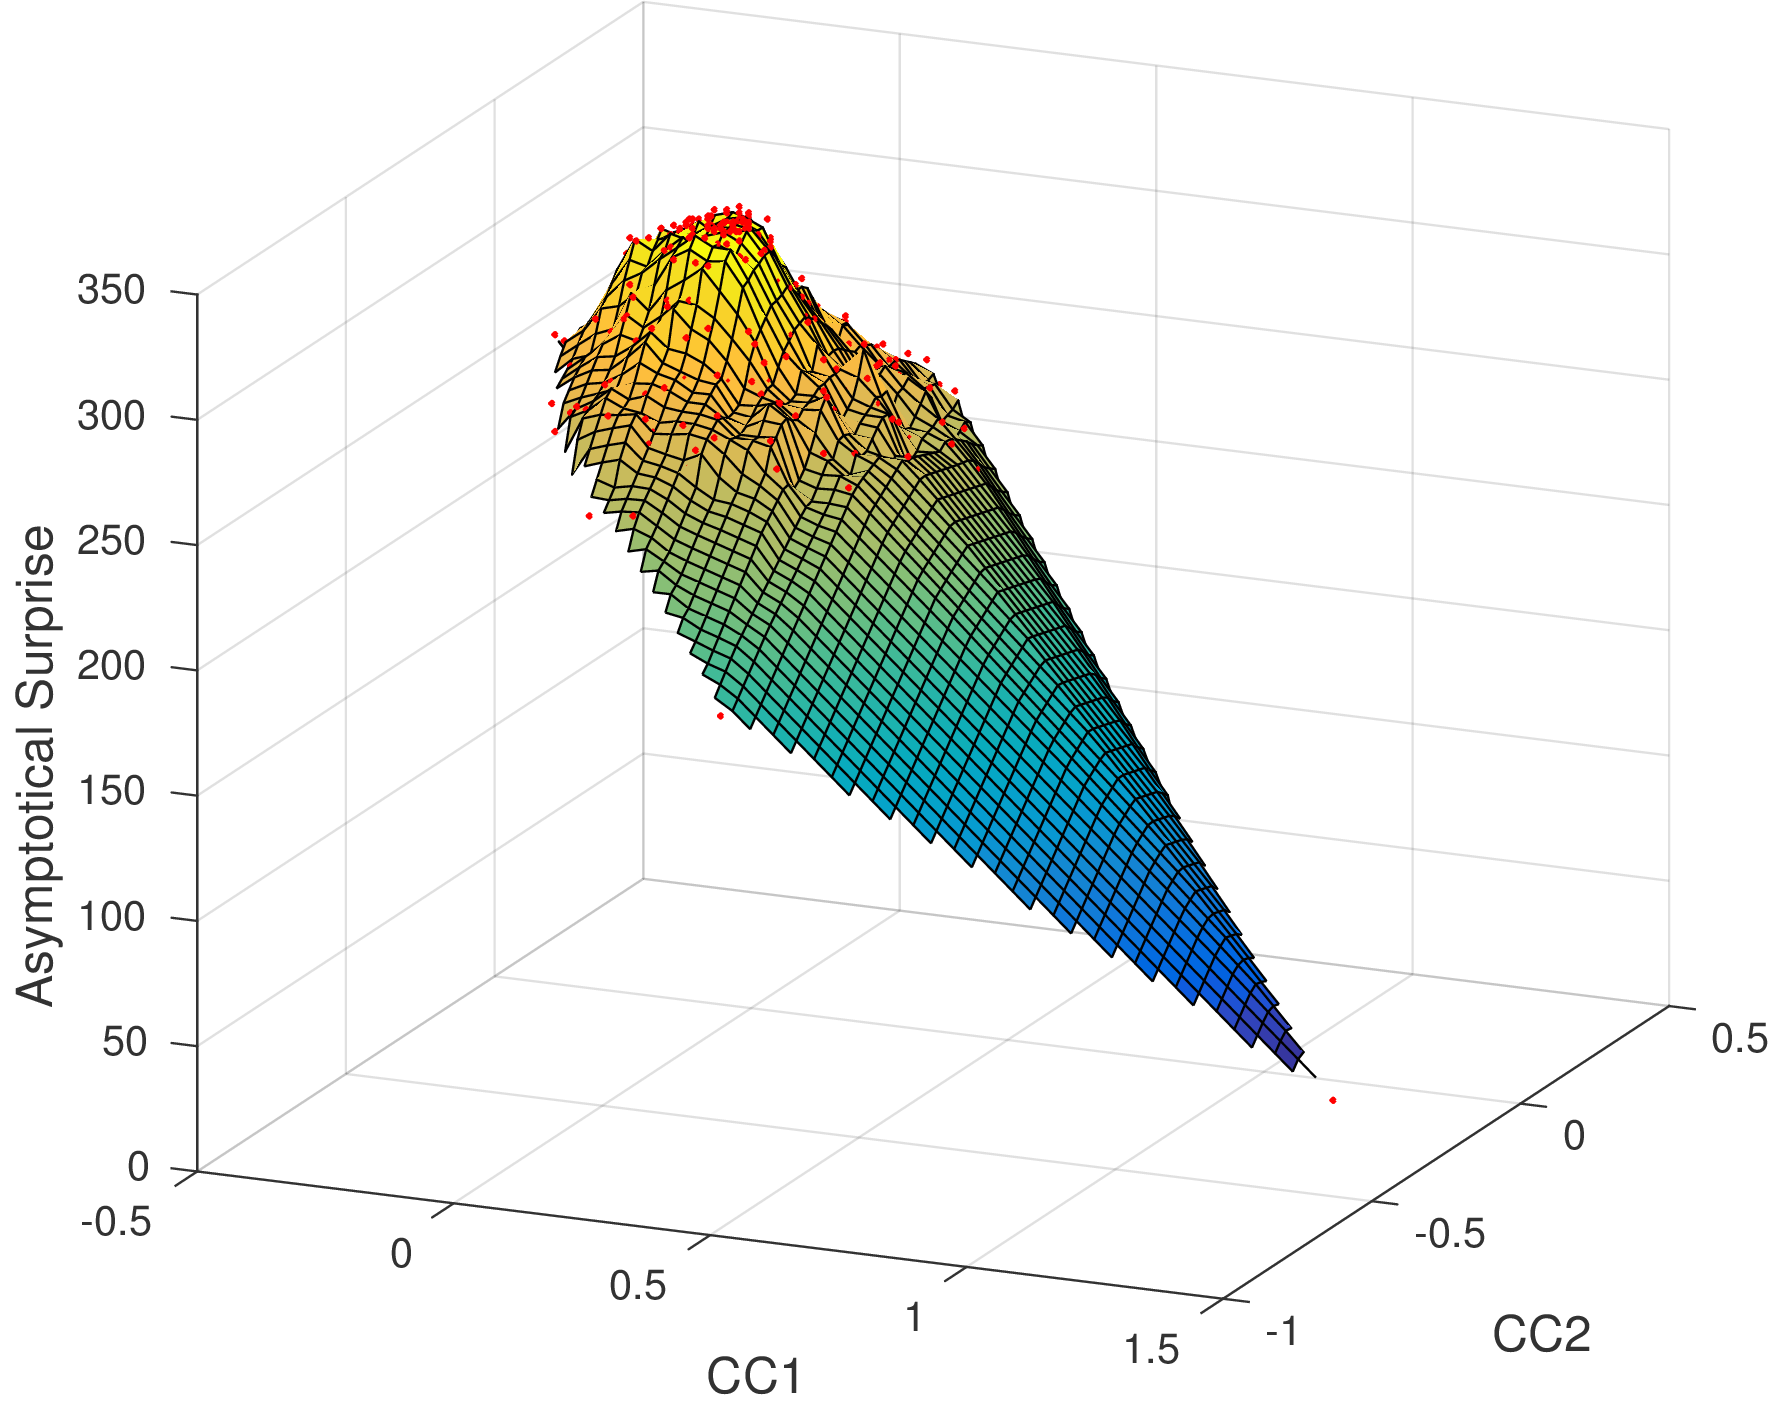
\includegraphics[width=1.0\textwidth]{images/filtered_asymp_surp_ring_cliques_5_24_200.png}
\caption{Degeneracy landscape of Asymptotical Surprise on a ring of clique model with 24 cliques of 5 nodes.}
\label{fig:degeneracy_asymptotical_surprise}
\end{figure}

%%%%%%%%%%%%%%%%%%%%%%%%%%%%%%%%%%%%%%%%%%%%%%%%%%%%%%%%%%
%%%%%%%%%%%%% RUNNING TIME ANALYSIS OF PACO %%%%%%%%%%%%%%
%%%%%%%%%%%%%%%%%%%%%%%%%%%%%%%%%%%%%%%%%%%%%%%%%%%%%%%%%%
\subsection{Running time analysis of PACO}
I applied PACO on a full-resolution voxelwise connectivity matrix with 51,653 nodes and almost 2 million edges.
PACO took 14 minutes for a single repetition on a server with Intel Xeon E5-2643@ 3.40 Ghz CPU and 256 GB ram.
I estimated that 2000 repetitions of PACO would take approximately 2.5 weeks on this server.
I've also tried to run PACO on a standard office PC with 16 GB memory and an Intel Core i7: it took almost 40 minutes.
It's important to notice that the running time of PACO is mainly determined by the computation of Jaccard indexes in the initial step.
The running time for this computation is in the order of $O(nd^2)$ where $n$ is the number of nodes and $d$ is the average degree of nodes.
On a desktop workstation with a 2.5 GHz CPU, PACO runs in some tenths of seconds on a single repetition for a graph of around 600 nodes with a density close to 10\%, typical of brain networks.
A small benchmark of PACO running times on a desktop workstation is shown in Figure~\ref{fig:paco_benchmark}, where we found optimal Surprise partitions of a LFR network with the parameters described in the text but increasing number of nodes.

\begin{figure}[!htb]
\centering
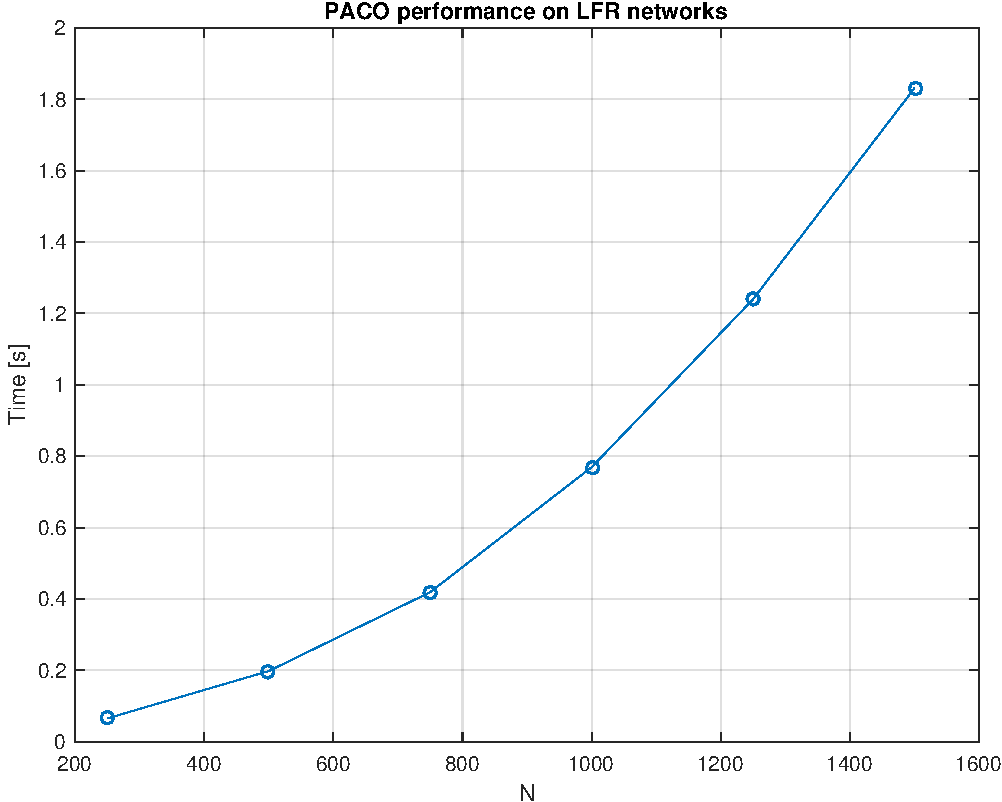
\includegraphics[width=0.5\textwidth]{images/paco_benchmark.pdf}
\caption{Performance of PACO on a LFR network with parameters}
\label{fig:paco_benchmark}
\end{figure}

%%%%%%%%%%%%%%%%%%%%%%%%%%%%%%%%%%%%%%%%%%%%%%%%%%%%%%%%%%
%%%%%%%%%%%%% PACO REPRODUCIBILITY %%%%%%%%%%%%%%%%%%%%%%%
%%%%%%%%%%%%%%%%%%%%%%%%%%%%%%%%%%%%%%%%%%%%%%%%%%%%%%%%%%
\subsection{Reproducibility of PACO optimal solutions}
In order to get a better idea of how fast the PACO method converges to a maximum, I have plotted in Figure~\ref{fig:paco_variability} the optimal value of Asymptotical Surprise over the 10000 runs for one instance of the LFR network, and for the resting state data-set presented in the section~\ref{sec:restingstatedataset}.
From these graphs, it appears that 2000 runs may be sufficient to reach stable community detection for the experimental data-set.
A near-optimum value is reached earlier for the LFR network, but it should be noted that I have taken an instance of the synthetic network with no-noise added.

\noindent\begin{figure}[!htb]
\centering
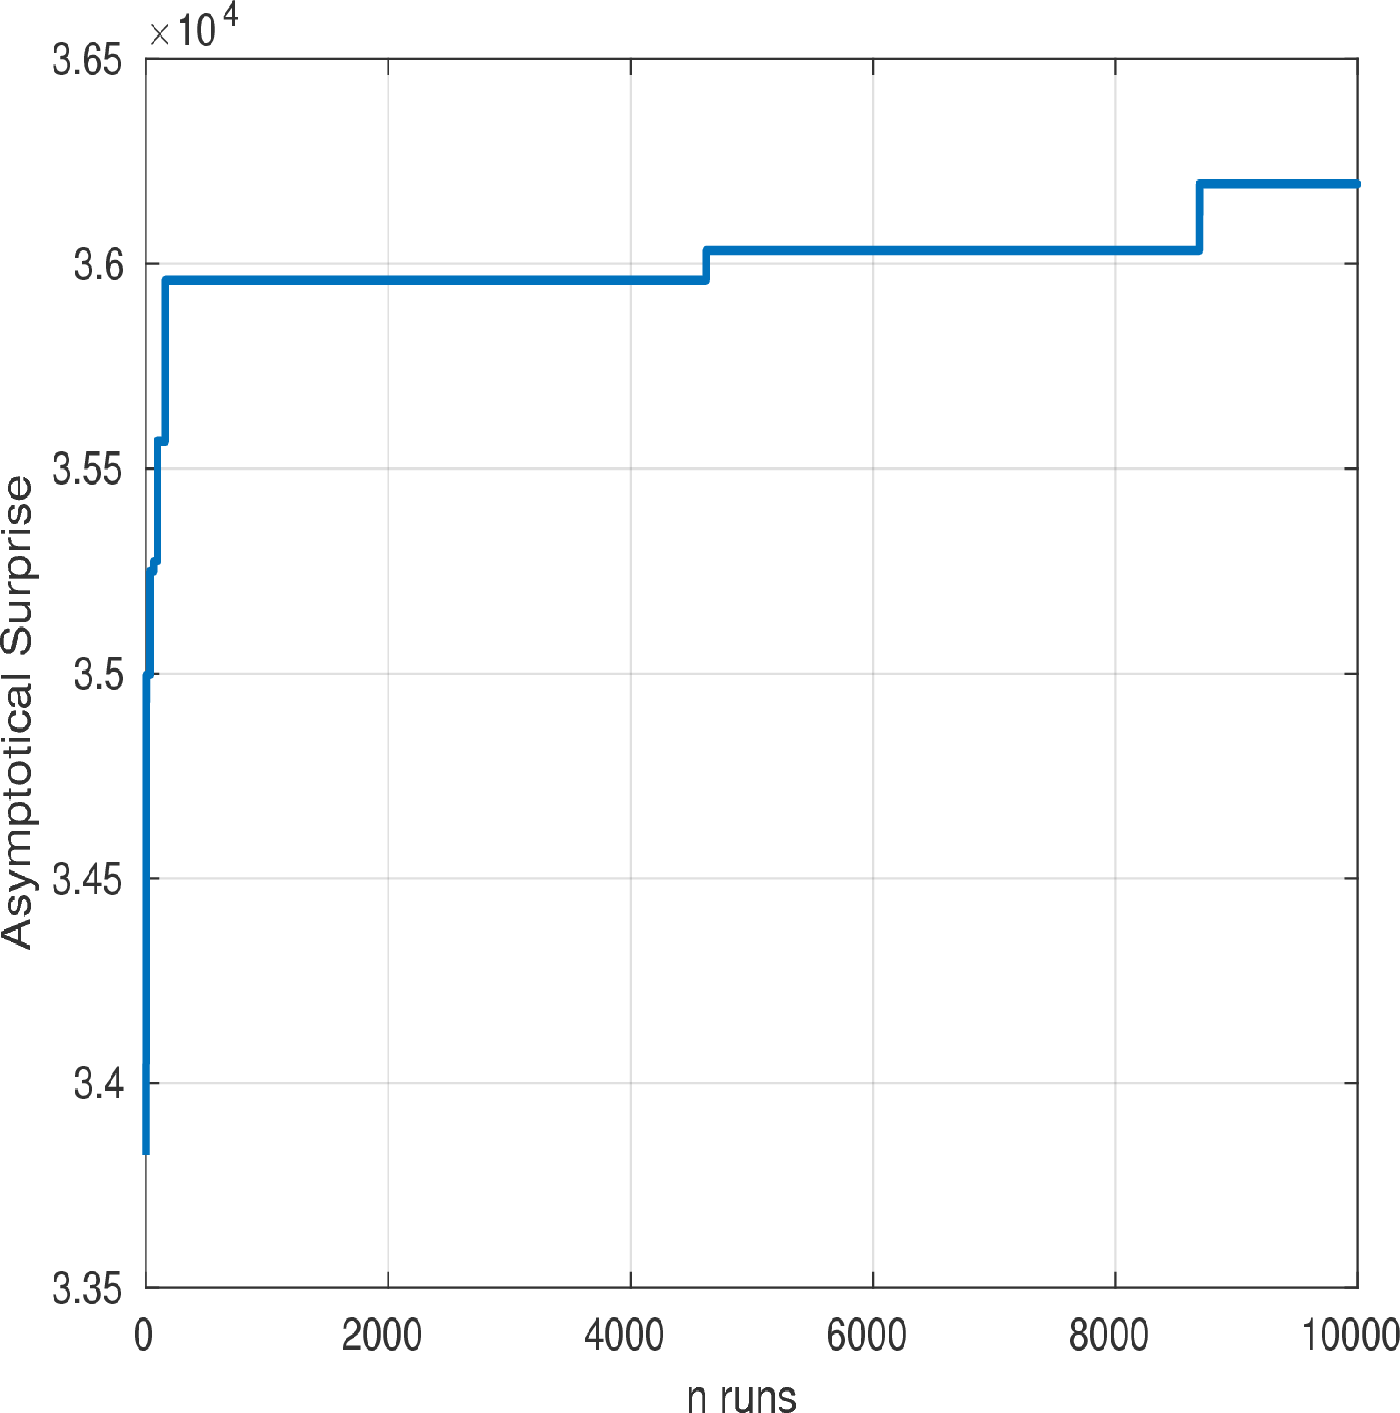
\includegraphics[width=0.45\textwidth]{images/paco_variability_nreps_lfr.png}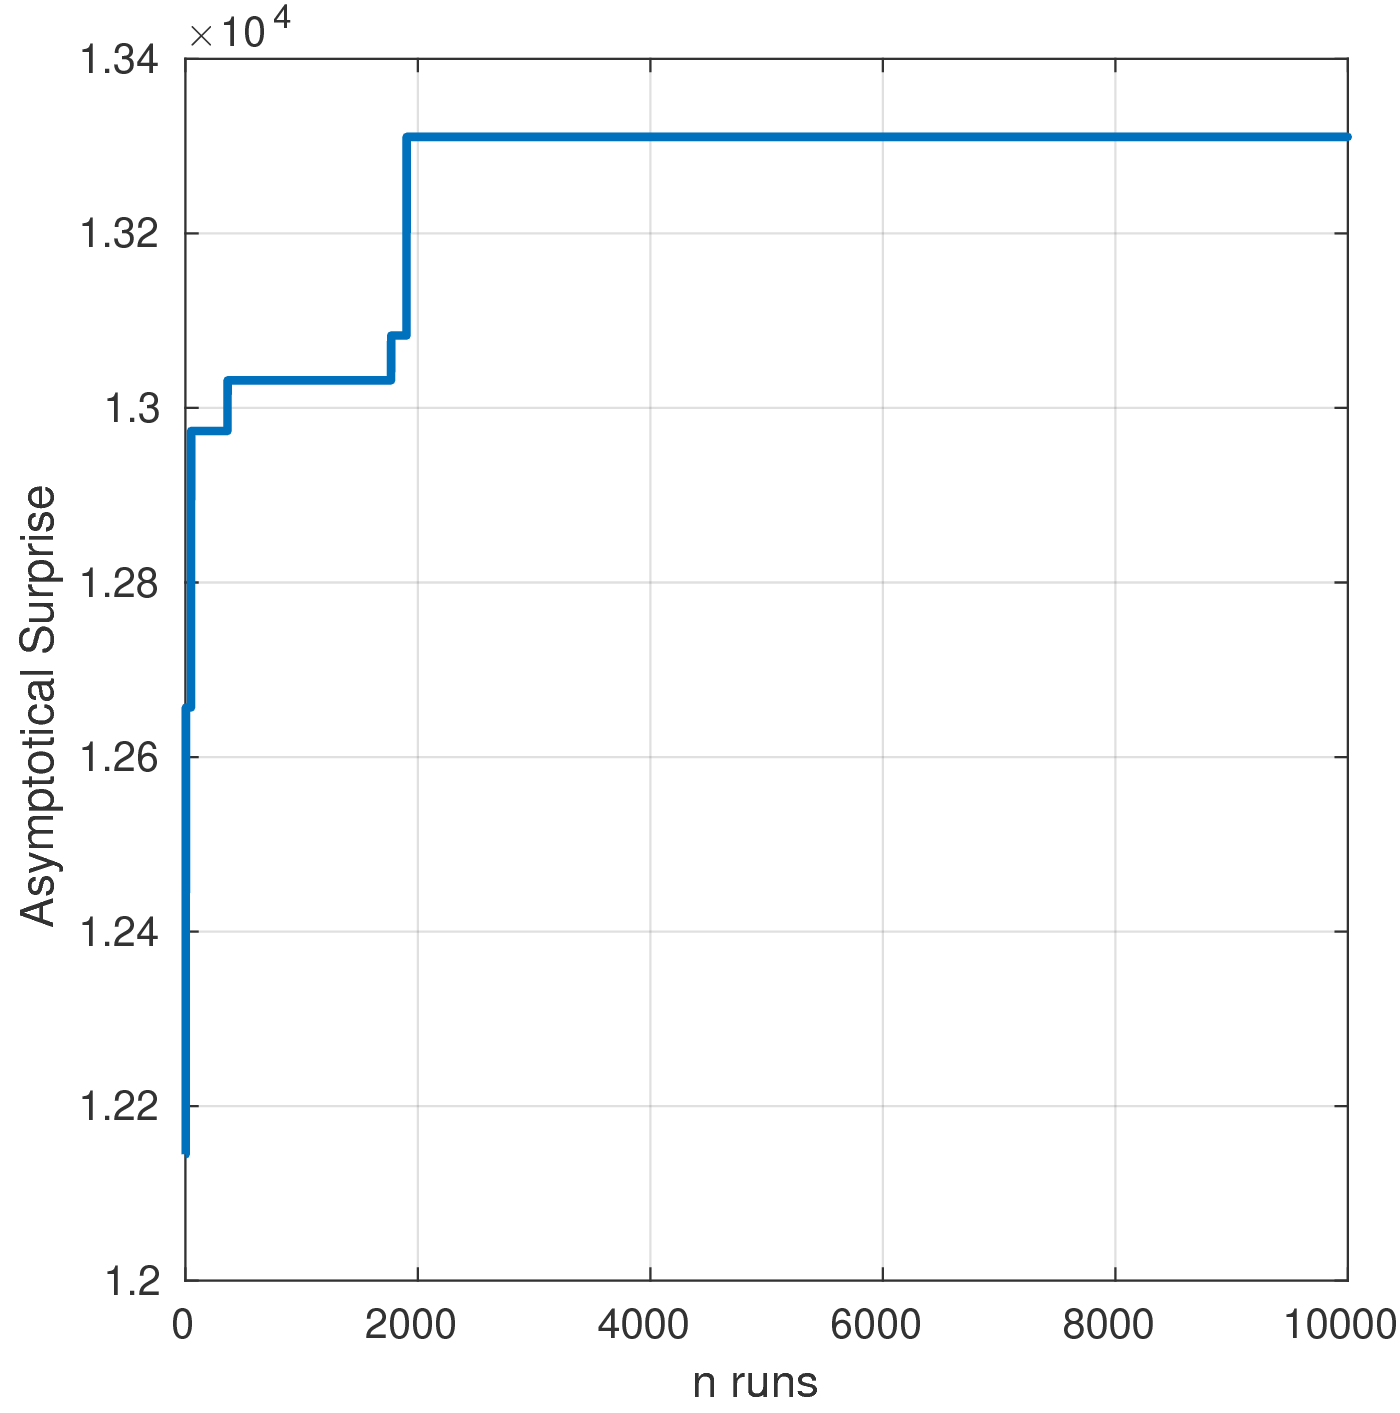
\includegraphics[width=0.45\textwidth]{images/paco_variability_nreps_bullmore.png}
\caption{Maximum value of Asymptotical Surprise with respect to number of repetitions on a LFR networks (left panel) and on a resting state network as in~\cite{crossley2013a}.}
\label{fig:paco_variability}
\end{figure}


%%%%%%%%%%%%%%%%%%%%%%%%%%%%%%%%%%%%%%%%%%%%%%%%%%%%%%%%%%
%%%%%%%%%%%%%%%%%%% BENCHMARKING PACO %%%%%%%%%%%%%%%%%%%%
%%%%%%%%%%%%%%%%%%%%%%%%%%%%%%%%%%%%%%%%%%%%%%%%%%%%%%%%%%
\subsection{Benchmarking PACO}
Among the two most important parameters in the LFR benchmark are the topological and weights mixing coefficients. 
The topological mixing coefficient $\mu_t$ is the average ratio of intra-cluster neighbors divided by the number of inter-cluster neighbors, as defined in~\cite{lancichinetti2008}.
The weights mixing coefficient is defined as the average ratio of node intra-cluster strength and inter-cluster strength, as defined in~\cite{lancichinetti2009a}.
I explored the effects of these parameters on the ability of PACO to retrieve the planted structure in the network.
I set $\mu_t=\mu_w$, as setting $\mu_w$ greater than $\mu_t$ would introduce inconsistency in the relative number and weight of the edges, with intermodule edges carrying the largest weights.

I analyzed the performance of Newman's Modularity, Infomap and PACO on LFR networks where I varied the topological and weights mixing coefficients.
In Figure~\ref{fig:avgmutmuw} the performance of the three methods is comparable in terms of NMI, with a faster decay of NMI for InfoMap and Newman compared to PACO for large $\mu_t$.

\begin{figure}[!htb]
\centering
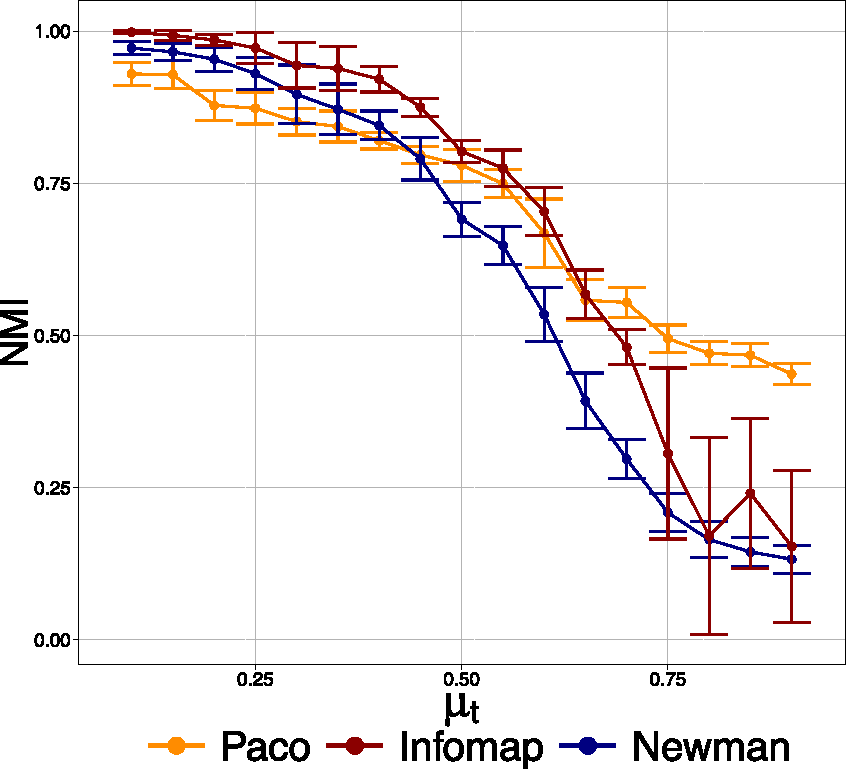
\includegraphics[width=0.65\textwidth]{images/avg_nmi_allmethods_lfr_errorbars.pdf}
\caption{NMI of the retrieved vs planted partition of an LFR network as a function of $\mu_t=\mu_w$ for the three community detection methods.}
\label{fig:avgmutmuw}
\end{figure}

%%%%%%%%%%%%%%%%%%%%%%%%%%%%%%%%%%%%%%%%%%%%%%%%%%%%%%%
%%%%%%%%%% SYNTHETIC BENCHMARK NETWORKS %%%%%%%%%%%%%%%
%%%%%%%%%%%%%%%%%%%%%%%%%%%%%%%%%%%%%%%%%%%%%%%%%%%%%%%
\section{Synthetic benchmark networks}
One important finding in~\cite{nicolini2016} is that brain networks are organized in modules with heterogeneous size distributions.
I implemented this property in our two types of benchmark networks.
For the first test, I generated a ring of cliques with $300$ nodes, and sizes of the cliques sampled from a power-law with exponent $\tau_c=2$, minimum and maximum clique size respectively $\min_c=5$, $\max_c=50$.
For each subject of the sample, I synthesized $150$ time-points for each node using the \texttt{neuRosim R} package~\cite{neurosim2011}.
I set the baseline value of all the time series to $100$~\cite{welvaert2013}.

Finally, I correlated the original synthetic time series $\mathbf{X}$ by multiplication with the matrix $\mathbf{L}$, obtained the correlated time series $\mathbf{Y}$ and added Rician noise~\cite{Gudbjartsson1995} to $\mathbf{Y}$ independently for each area.
The simulated data $\mathbf{Y}$ did not include slow drift components, simulated physiological noise, nor spatial noise.
The average SNR is defined as $\textsc{SNR}=\bar{S}/\sigma_N$ where $\bar{S}$ is the average magnitude of the signal and $\sigma_N$ is the standard deviation of the noise~\cite{kruger2011}.

In order to be more exhaustive and extend the validity of results, I repeated the same procedure on weighted LFR networks with $N=600$ nodes, sampling nodes degree from a power-law with exponent $\tau_d=2$, average degree $\left<k\right>=12$ and maximum degree $\max_k=50$.
I set the topological and weights mixing coefficients, i.e. the average fraction of intra-cluster and inter-cluster degree and strengths, to $\mu_t=0.1$ and $\mu_w=0.1$, respectively.
Planted community sizes ranged from $5$ to $50$ nodes and were sampled from a power law with exponent $\tau_c=1$.

Group-level correlation matrices were computed by Fisher-transforming and averaging individual instances of the above matrices.
Sparsification was obtained by removing edges with weights below the most stringent threshold that maintained the network connectedness, a procedure known as percolation analysis~\cite{gallos2012,bardella2016a,alexander-bloch2010}.
This approach measures the size of the largest connected component of the network upon iterative removal of the weakest edges and enables data-driven determination of the optimal sparsification threshold that preserves network structure and connectedness while removing potentially spurious correlations.

The community structure of the resulting weighted sparsified matrices was detected by Asymptotical Surprise optimized with PACO and compared against two widely used methods, Infomap~\cite{rosvall2008} and Newman's Modularity~\cite{blondel2008,newman2006}, that are affected by the resolution limit, albeit to different extents.
In Newman's Modularity, the size of the smallest detectable cluster is of the order of the square root of the number of edges in the entire network~\cite{fortunato2007}, while Infomap has a limit that depends on the overall number of inter-cluster edges~\cite{kawamoto2015}.
Here I used the Louvain implementation available in the Brain Connectivity toolbox~\cite{rubinov2010} and the Infomap implementation available in the \texttt{igraph-0.7.1} package~\cite{igraph2006}.

For all methods, including PACO, I launched $10,000$ independent runs, and picked the membership corresponding to the partition with the best value of the fitness function, the maximum for Modularity and Asymptotical Surprise, the minimum for Infomap.
As discussed in the previous chapter, sections~\ref{sec:degeneracy},~\ref{sec:degeneracy_surprise},~\ref{sec:degeneracy_asymptotical_surprise}, degeneracy of nearly-optimal solutions does not appear to severely affect Surprise or Asymptotical Surprise, and a consensus approach is not deemed necessary for these functions.
This analysis supports the choice of selecting the solution with the highest value of the fitness function.

%%%%%%%%%%%%%%%%%%%%%%%%%%%%%%%%%%%%%%%%%%%%%%%%%%%%%%%
%%%%%%%%%%%% MEASURES OF PARTITION QUALITY %%%%%%%%%%%%
%%%%%%%%%%%%%%%%%%%%%%%%%%%%%%%%%%%%%%%%%%%%%%%%%%%%%%%
\subsection{Measures of partition quality}
For each method, we analyzed the level of agreement of the detected community structure against the planted one in terms of Normalized Mutual Information (NMI)~\cite{danon2005}.
Additionally, we used two different coefficients of similarity between partitions: Sensitivity and Specificity. 

To this end, we quantified the confusion matrix $\mathbf{C}$ between the detected and planted modules. Each element $C_{ij}$ is the number of nodes in the planted community $i$ that appear in the detected community $j$.
For each planted community we scored as true positives (TP) the nodes correctly identified as belonging to the ground-truth community, and as false positives (FP) the nodes wrongly assigned to a community; similarly false negatives (FN) were nodes wrongly classified in different communities and true negatives (TN) the nodes correctly classified as out of the community.
Sensitivity, defined as $TP/(TP+FN)$, decreases with increasing number of False Negatives. Specificity instead is defined as $TN/(TN+FP)$ and decreases when many nodes are wrongly assigned in the same community.

%%%%%%%%%%%%%%%%%%%%%%%%%%%%%%%%%%%%%%%%%%%%%%%%%%%%%%%
%%%%%%%%  PACO BENCHMARK ON SYNTHETIC NETWORKS %%%%%%%%
%%%%%%%%%%%%%%%%%%%%%%%%%%%%%%%%%%%%%%%%%%%%%%%%%%%%%%%
\section{PACO benchmark on synthetic networks}
I compared the quality of the partitions of the synthetic benchmark networks obtained by Asymptotical Surprise with those of Infomap~\cite{rosvall2008} and Newman's Modularity~\cite{newman2006,blondel2008}. Figure~\ref{fig:nmisensitivityspecificityringclique} shows Normalized Mutual Information, Sensitivity and Specificity of the three methods applied to the ring of cliques for different sample sizes and SNRs; no-noise condition is represented as ``Inf''.
This model network was constructed to test the ability of the three methods to retrieve heterogeneous community structures under various noise conditions.

As expected, all methods showed better performance with increasing SNR and number of subjects, as noise and intersubject variability introduce spurious edges that hinder the ability to retrieve the planted structure.
Partitions obtained with Newman's modularity showed the lowest NMI with respect to the planted partition under all conditions.
Sensitivity of Newman's modularity did not exceed $0.75$ even for high SNRs and a large number of subjects, a consequence of its stronger resolution limit.
For this network, Infomap performed substantially better in terms of NMI against the planted partition, with a Sensitivity that was superior to that of Modularity across the spectrum of conditions.

Asymptotical Surprise showed highest NMI and Sensitivity across conditions, consistent with its resolution-limit-free behavior. It proved superior in terms of NMI and Sensitivity in the low SNR regimes, and in the presence of relatively large intersubject variability as mimicked by the generation of different instances of the ring of cliques.
Specificity of Asymptotical Surprise was not inferior to the other methods under all conditions, thus ruling out increased vulnerability to False Positives, at least in this particular model network.
\begin{figure}[!htb]
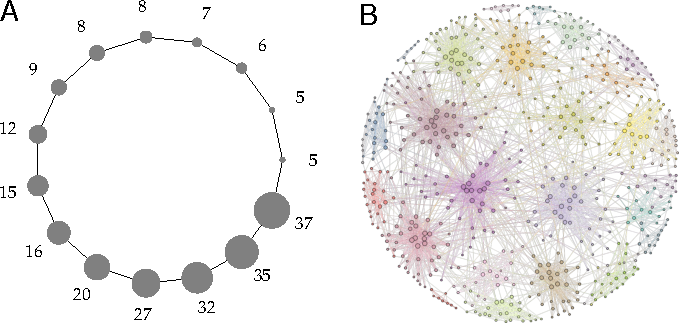
\includegraphics[width=1\textwidth]{images/pacopaperfigure1.pdf}
\caption{The two benchmark networks used in this study, laid out. (A) is a power-law ring of cliques, where cliques present different sizes sampled from a power-law distribution;
(B) is the layout of an LFR network with parameters $N=600$, $\left< k \right>=12$, $\max_k=50$, $\mu_t=0.1$, $\mu_w=0.1$, $\min_c=5$, $\max_c=50$.
The layout of (B) was generated with the graph-tool library~\cite{peixoto_graph_tool_2014}.}
\label{fig:lfrringclique}
\end{figure}
\begin{figure}[!htb]
\includegraphics[width=\textwidth]{images/pacopaperfigure4.pdf}
\caption{NMI, Sensitivity and Specificity of the three community detection algorithms applied to a power-law ring of clique network. SNR indicates Signal to Noise Ratio, and Inf the situation with a network structure unperturbed by noise. Number of Subjects indicates the different number of instances used to generate the group level network.}
\label{fig:nmisensitivityspecificityringclique}
\end{figure}
Comparable results were obtained for the LFR network (Figure~\ref{fig:nmisensitivityspecificitylfr}), a model graph that replicates the distribution of nodal degree observed in many real-world networks, including those representing brain functional connectivity.
All three methods showed similar values of NMI for high SNR and a large number of subjects, with a plateau reaching maximum Sensitivity with a group sample bigger than $20$ and SNR above $30$.
Sensitivity was only slightly worse for Modularity, but it should be noted that for the LFR network the size distribution of the planted modules was narrower than for the ring of cliques (Figure~\ref{fig:lfrringclique}), thus making the resolution limit less evident.
\begin{figure}[!htb]
\includegraphics[width=\textwidth]{images/pacopaperfigure5.pdf}
\caption{NMI, Sensitivity and Specificity of the three community detection algorithms applied to Lancichinetti-Fortunato-Radicchi (LFR) networks. SNR indicates Signal to Noise Ratio, and Inf the situation with a network structure unperturbed by noise. Number of Subjects indicates the different number of instances used to generate the group level network.}
\label{fig:nmisensitivityspecificitylfr}
\end{figure}
In the lower SNR regime, Asymptotical Surprise presented the best performance in terms of NMI and Sensitivity, with a slower decay for decreasing SNR. 
Specificity was almost equivalent across the three methods, with a quick convergence to the maximum value of 1 for high SNR and good performance (around $0.97$) for low SNR.
Asymptotical Surprise presented a faster decay with decreasing SNR.
However, it should be noticed that the scale of Specificity has a very narrow range ($0.97$-$1.00$), and the differences between the three methods were relatively small.

Consensus analysis applied to Newman's Modularity to assess the potential effects of the degeneracy of nearly optimal solutions did not show substantial differences in the comparison with the other methods.
Notably, Infomap showed a large variability in Accuracy for lower SNRs and number of subjects.
Under closer examination, however, it appeared that the increased variance for Infomap was due to occasional runs in which the algorithm only retrieved one or two large modules.
This is a known problem with Infomap and other algorithms based on random walks that depends on the need to parametrize the teleportation step in order to make the dynamics ergodic~\cite{lambiotte2012}.

For the sake of completeness, we also computed Accuracy and Matthew Correlation Coefficient for the same model networks.
As shown in Figure~\ref{fig:accmcc_cliques}, Accuracy of Newman's Modularity is lower for small SNRs and number of subjects and in any case it does not reach 100\% of true positives classification even in the no-noise condition. Infomap accuracy is high for SNR greater than 20, largely independent on the number of subjects. The large variance of Infomap for low SNRs is due to the merging of all nodes in a single large community in a few runs, as discussed in the main text. Asymptotical Surprise, behaves well in terms of Accuracy and has the least variability across all methods, plateauing at 100\% for SNRs greater than 20 and more than 40 subjects.
In terms of MCC, Figure~\ref{fig:accmcc_cliques} shows that Asymptotical Surprise behaves comparably or better than Infomap.
Newman's modularity is the least performer, due to its resolution limit, and never reaches maximum MCC. Interestingly, Asymptotical Surprise slightly outperforms Infomap in terms of MCC in the single subject case in the no-noise condition.
The comparison of the three methos is similar in the case of the LFR benchmark, as shown in Figure~\ref{fig:accmcclfr}.
\begin{figure}[!htb]
\centering
\includegraphics[width=\textwidth]{images/figure3_supplementary.pdf}
\caption{Accuracy and Matthew correlation coefficient on the modified ring of clique benchmark.}
\label{fig:accmcc_cliques}
\end{figure}
\begin{figure}[!htb]
\centering
\includegraphics[width=\textwidth]{images/figure4_supplementary.pdf}
\caption{Accuracy and Matthew correlation coefficient on the LFR benchmark.}
\label{fig:accmcclfr}
\end{figure}

Altogether, the picture that emerges from the analysis of Accuracy and MCC is entirely consistent with the results shown in this section.

%%%%%%%%%%%%%%%%%%%%%%%%%%%%%%%%%%%%%%%%%%%%%%%%%%%%%%%%%%%%%%%%%%%%%%%%%%%
%%%%%%%%% ASYMPTOTICAL SURPRISE ON RESTING STATE DATASET %%%%%%%%%%%%%%%%%
%%%%%%%%%%%%%%%%%%%%%%%%%%%%%%%%%%%%%%%%%%%%%%%%%%%%%%%%%%%%%%%%%%%%%%%%%%%
\section{Asymptotical Surprise on resting state dataset}
Figure~\ref{fig:partitioncomparison} shows a comparison between the modular structure of the resting state fMRI dataset obtained with Newman's Modularity, Infomap and Asymptotical Surprise.
For each method, I had $10,000$ independent runs and picked the partition with the best value of the respective fitness functions ($Q=0.4967$, $\mathcal{L}=8.5173$, $S_a=5925.3$, for Modularity, Infomap and Asymptotical Surprise, respectively).
The three methods showed significantly different partitions (relative NMIs in Table 1), with a number of detected communities of 10, 19 and 47 for Modularity, Infomap and Asymptotical Surprise, respectively.
Interestingly, Modularity detected a relatively uniform size distribution, consistent with the intrinsic scale built into the fitness function.
Infomap showed a wider distribution of module sizes, with number of nodes ranging between 156 and 3, while Surprise showed the largest spread, and included communities as small as single nodes (singletons).
\begin{figure}[!htb]
\includegraphics[width=\textwidth]{images/pacopaperfigure6.pdf}
\caption{Adjacency matrix of the resting state functional connectivity network. The node indices have been reordered by module membership in each graph, and the red lines highlight the community structures obtained by A) Louvain-Newman's Modularity ($Q=0.4967$); B) Infomap ($L=8.5173$); C) Asymptotical Surprise ($S_a=5925.28$).}
\label{fig:partitioncomparison}
\end{figure}

Figure~\ref{fig:cervellini4x4} shows the 16 largest modules detected by Asymptotical Surprise, ranked by number of nodes comprised in each community. 
The first and largest module (Figure~\ref{fig:cervellini4x4}A) includes the pre- and post-central gyri, part of the supramarginal gyrus and supplementary motor area.
The second community (Figure~\ref{fig:cervellini4x4}B) consists largely of nodes belonging to the occipital lobe: the visual areas and the surrounding calcarine sulcus, the lingual and fusiform gyrus.
The third module (Figure~\ref{fig:cervellini4x4}C) reflects the Default Mode Network, spanning the temporo-parietal cortex, the medial prefrontal cortex and the posterior cingulate/precuneus.
The nodes involved in the executive frontal functions form the fourth largest community.
Interestingly, nodes in the communities D, E, G are the major players that take part in the so-called fronto parietal attentional network~\cite{markett2014}.
The auditory network, comprising temporal areas, was detected as a distinct community (Figure~\ref{fig:cervellini4x4}F).
Deeper structures emerge as separate modules in Figure~\ref{fig:cervellini4x4}H, with subcortical areas including the basal ganglia, i.e. putamen, globum pallidum, caudate nucleus and the whole thalamus.
The hippocampus and the parahippocampal gyrus were identified as separate communities (O and P).
Additional, smaller substructures are shown in the third and fourth row of Figure~\ref{fig:cervellini4x4}, including the Supplementary Motor Area (Figure~\ref{fig:cervellini4x4}J) and the orbital (Figure~\ref{fig:cervellini4x4}M) and orbitofrontal (Figure~\ref{fig:cervellini4x4}I) modules, containing nodes from Brodmann area 47.

\begin{figure}[!htb]
\includegraphics[width=\textwidth]{images/pacopaperfigure7.pdf}
\caption{Sixteen largest modules found by Asymptotical Surprise Maximization in the resting state network overlaid on an MRI brain template. The modules are ranked by decreasing size, and named after corresponding functional networks previously identified by multivariate analysis of resting state fMRI data, or by the comprised anatomical districts.}
\label{fig:cervellini4x4}
\end{figure}
\begin{figure}[htb]
\centering
\includegraphics[width=1\textwidth]{images/figure_cervellini_Louvain_Q_0_49674.png}
\caption{First largest 8 modules of the optimal partition as found by Newman's Modularity, with a value of the Modularity $Q=0.4967$. Module 9 is not shown as it consists of a single node.}
\label{fig:newmancervellini}
\end{figure}
\begin{figure}[htb]
\centering
\includegraphics[width=1\textwidth]{images/figure_cervellini_infomap_L_8_5173.png}
\caption{First largest 16 modules of the optimal partition as found by Infomap, with a value of the description length $L=8.5173$.}
\label{fig:infomapcervellini}
\end{figure}

Newman's Modularity retrieved four large, relatively uniform communities, corresponding to the Default Mode Network, the central network, occipital and frontoparietal networks.
This is in keeping with previous studies using Modularity optimization by spectral decomposition~\cite{crossley2013a}, and consistent with the strong resolution limit that affects this method.
Additionally, a few smaller modules were found by Louvain optimization of Newman's Modularity, corresponding to the basal ganglia, the hippocampal/parahippocampal formation and two asymmetrically distributed subcortical clusters.

Infomap identified 19 communities of various sizes, also shown in Figures~\ref{fig:infomapcervellini} and \ref{fig:infomapcervellini}.
The largest modules showed a close correspondence with those identified by Asymptotical Surprise, albeit with some notable differences.
By way of example, the largest component includes the motor-sensory and auditory modules, identified as separate communities by Asymptotical Surprise.
The Default Mode Network retrieved by Infomap includes parts of the temporal cortices that are not normally associated with the DMN.
Similarly, hippocampus and the parahippocampal modules were merged by Infomap, and resolved as individual modules by Asymptotical Surprise.
Other modules, including the visual, associative and executive networks (C, E and F in Figure~\ref{fig:infomapcervellini}, respectively) were qualitatively very similar to those identified by Asymptotical Surprise.

Altogether, the picture that emerges is consistent with the idea that the resolution limit is more severe in Newman's Modularity than in Infomap, and that Asymptotical Surprise presents the best resolving power among the three methods in a real-world network with finite SNR and variability as the resting state functional connectivity network used for this study.

\subsection{Hub classification}
Maps of the anatomical distribution of the participation coefficient and within module degree show substantial differences between the three community detection methods (Figure~\ref{fig:hubclassification}), resulting in discrepancies in the identification of the connector hubs for the same functional connectivity network.

Figure~\ref{fig:hubclassification_threshold} shows the nodes with simultaneously high values of participation coefficient and within module degree (connector hubs, according to the Guimera and Amaral's classification).
All three methods pinpoint connector hubs in the superior, superior medial and middle frontal areas, as well as in the supplementary motor area.
However, substantial differences are observed for other hub regions. The partition of Asymptotical Surprise localizes connector hubs in the Temporal Middle and Frontal Middle gyri, as well as in the Rectus, Middle Cingulate Cortex, Lingual gyrus and in the Precuneus.

Community detection by InfoMap results in the identification of hubs that are partially consistent with either of the two other methods, in keeping with the idea that its resolution limit is less severe than for Newman's Modularity.
Altogether, these findings indicate that node role classification is method-dependent, and may be affected by the resolution limit.

\begin{figure}[!htb]
\includegraphics[width=\textwidth]{images/pacopaperfigure8.pdf}
\caption{Anatomical distributions of the participation coefficient and within-module degree z-score for the resting state functional connectivity network partitioned by the three community detection methods.}
\label{fig:hubclassification}
\end{figure}
\begin{figure}[!htb]
\includegraphics[width=0.6\textwidth]{images/pacopaperfigure9.pdf}
\caption{Nodes presenting simultaneously large values of the participation coefficient and within-module degree (larger than 0.6 and 1.5, respectively) for the three community detection methods. These nodes are thought to represent the connector hubs responsible for the integration of the networks's modules.
}
\label{fig:hubclassification_threshold}
\end{figure}

%%%%%%%%%%%%%%%%%%%%%%%%%%%%%%%%%%%%%%%%%%%%%%%%%%%%%%%%%%%%%%%%%%%%%%%%%%%%%%
%%%%%%%%%%%%% VALIDATION OF ASYMPTOTICAL SURPRISE IN MODEL NETWORKS %%%%%%%%%%
%%%%%%%%%%%%%%%%%%%%%%%%%%%%%%%%%%%%%%%%%%%%%%%%%%%%%%%%%%%%%%%%%%%%%%%%%%%%%%
\subsection{Validation of Asymptotical Surprise in model networks}
The performance of Asymptotical Surprise optimization by PACO was assessed in model graphs with a built-in community structure, and compared with two established community detection methods. We have chosen two synthetic benchmark networks, the ring of cliques and the LFR network.

The ring of cliques presents a clear-cut modular structure by construct, with modules corresponding to complete subgraphs of variable sizes sampled from a power-law distribution. 
This toy network proved useful to assess the effects of the resolution limit in the presence of a wide distribution of cluster sizes. The effects of this limit were particularly apparent for Newman's Modularity (Figure~\ref{fig:nmisensitivityspecificityringclique}), that showed poor Sensitivity even for noiseless rings of cliques, plateauing at a value of $0.75$.
This is consistent with the findings of~\cite{fortunato2007}, that showed that for Modularity the resolution limit is set by the square root of the total number of edges in the graph.
For Infomap, this limit is less severe and is determined by the number of inter-cluster edges~\cite{kawamoto2015}. Accordingly, the effects of the resolution limit were not apparent in this model network, where modules are sparingly connected by single edges.
Asymptotical Surprise presented the best performance, consistent with the idea that this cost function is quasi-resolution limit free~\cite{traag2015}.

However, real brain networks are characterized by heterogeneous distributions of node degree, with fat tails and power-law decays~\cite{bullmore2009}. Such heterogeneity is critical, as it determines some of the remarkable features of brain connectivity networks, including resilience to random failure and rich-clubness~\cite{vandenheuvel2011,vandenheuvel2013a}. To provide a more realistic benchmark, we used the Lancichinetti-Fortunato-Radicchi algorithm~\cite{lancichinetti2008}, that makes it possible to generate networks with realistic and tunable power law degree distribution and community sizes.

For LFR networks, the difference in performance in the low-noise regime was more nuanced for the three methods compared in this study, possibly a result of a fuzzier community structure of the LFR network compared to the ring of cliques, and of the narrower distribution of cluster sizes. However, the picture appears different when noise and intersubject variability were injected into the network structure.

Noise and other sources of variability in the data can significantly affect the structure of the resulting network representation.
Noisy fMRI time-courses, for example, may introduce spurious correlations in brain functional connectivity networks.
This problem may be particularly relevant for methods endowed with high resolution, like Asymptotical Surprise, that may be more vulnerable to False Positives generated by the mis-assignment of peripheral nodes, particularly in small clusters. Hence, the resolving power of community detection methods should be gauged against Specificity, which may be affected by noise in the distribution of edges that define the network's structure.
However, to the best of our knowledge, this aspect has never been considered in the existing literature assessing the performance of community detection algorithms as applied to the study of brain connectivity.

To this end, we have devised methods to inject noise, with amplitude and spectral distribution that mimic those of experimental noise, into networks with a well defined planted structure. Moreover, we have generated different instances for each network, corresponding to different subjects in a group, to account for intersubject variability that occurs in typical neuroimaging studies. 

Unsurprisingly, for all methods and networks, detection of the planted structure improved with decreasing levels of noise, and with increasing number of subjects in the study.
However, Asymptotical Surprise appeared to provide a superior performance in terms of NMI and Sensitivity to the planted structure for lower SNRs in both types of networks, while its Specificity was in line with that of resolution-limited methods like Newman's and Infomap (Figures \ref{fig:nmisensitivityspecificityringclique},\ref{fig:nmisensitivityspecificitylfr}).
This rules out the idea that the higher sensitivity to small clusters of Asymptotical Surprise may be detrimental in noisy networks, making it more vulnerable to small, spurious modules.

\subsection{Asymptotical Surprise optimization on resting state networks}
Application of Asymptotical Surprise maximization to a group-level, resting state functional connectivity network from the brains of $27$ healthy subjects revealed a heterogeneous distribution of modules, with large and small modules coexisting in the optimal partition.
This is in keeping with previous findings with binary Surprise~\cite{nicolini2016}.
These modules closely reflect functional networks reported in many studies using Independent Component Analysis or other multivariate methods, including the sensorimotor, visual, default mode, executive, and attentional networks.
Moreover, anatomically defined subcortical structures, like the hippocampus and parahippocampal formations emerged as independent moduli.

While this is entirely consistent with our understanding of the neurofunctional and anatomical organization of the human brain, the accuracy of Asymptotical Surprise in identifying these networks is notable.
Indeed, Surprise, like other graph-based community detection methods, divides networks into disjoint clusters of nodes on the basis of topological criteria.
While a correspondence between topological modularity and functional networks identified by, e.g. Independent Component Analysis, may be expected, it is not a given, for they are defined on different principles. Indeed, multivariate methods like ICA separate components on the basis of the statistical independence of the time-courses, and do not convey information regarding the mutual relationship between modules nor about their topological organization.

Previous studies applying resolution-limited methods like Newman's Modularity to the same dataset hereby analyzed~\cite{crossley2013a} found a few, large modules encompassing large-scale networks, but failed to identify finer, neurofunctionally plausible substructures like those shown in the present study. Infomap, on the other hand, proved sensitive to heterogeneously distributed clusters, thus implying that this method does not have an intrinsic scale, like Modularity and variations thereof based on the introduction of a resolution parameter. 
However, Asymptotical Surprise appears to provide superior performance in identifying small subnetworks, particularly in the presence of noise, thus suggesting that this method may represent a new standard for community detection in brain networks. It should also be noted that no symmetry constraint was imposed, and the symmetrical bilateral distribution of nodes in the retrieved modules arises entirely from Asymptotical Surprise optimization. 

Hierarchical clustering methods have been extensively applied to investigate the structure of brain connectivity networks, showing smaller and smaller clusters as the modules are iteratively subdivided~\cite{meunier2010}. Maximization of Asymptotical Surprise reflects the optimal cut through the dendrogram representing connectivity at these different levels of subdivision, and provides information on the optimal partition of the network. Hence, the heterogeneous distribution of cluster sizes retrieved by Asymptotical Surprise suggests that multiple scales of structure exist at the same level of the dendrogram.

Finally, abnormal functional connectivity has been observed in a number of neurological and psychiatric diseases, but the coarse resolution of methods like Newman's Modularity~\cite{fornito2015} may have not detected differences in the modular organization of networks in patients compared to healthy controls. The improved resolution and sensitivity to multiscale structure afforded by Asymptotical Surprise may provide a powerful means to assess the brain functional architecture in disease states, thus contributing a potential imaging-based marker and a key to interpret the functional effects of aberrant connectivity.
\subsection{Hub classification}
The presence of heterogeneously distributed modules in functional connectivity networks may have important consequences for our understanding of the brain functional organization. By way of example, it has been shown that highly connected nodes, or hubs, are critically important in brain connectivity networks, and may play different roles depending on their position and connectivity distribution within and between modules~\cite{bullmore2009}. Hubs that primarily connect to nodes within the same community are dubbed “provincial hubs”, and are thought to be responsible for the definition and stability of the modules. Conversely, hubs that connect different modules are referred to as “connector hubs” and ensure integration of the activity of the network. The classification of hubs strongly depends on the modular structure that is considered, and inaccurate partitioning due to the resolution limit can lead to the wrong interpretation of their role in the interplay between segregation and integration of brain function~\cite{bullmore2009}. The present study suggests that this may have been the case in previous studies, in which resolution limited methods characterized by an intrinsic scale have been used, and provides a solution that may enable more accurate classification of hubs and nodes.

The connector hubs identified by our three methods (Asymptotical Surprise, InfoMap and Newman) present some substantial differences, consistent with the idea that hub classification depends on community structure. These differences are particularly interesting in the light of the important role that connector hubs are thought to play in integrating information flow through the brain, and their putative role in brain disease \cite{crossley2014,stam2014}. By way of example, the Precuneus and the Cingulate Cortex are highlighted by Asymptotical Surprise, but not by Newman's Modularity, as connector hubs. These are two key elements of the Default Mode Network that have been consistently identified as vulnerable regions in neurological diseases~\cite{vandenheuvel2013a,buckner2009}. 
Community detection by resolution limited free methods should enable more accurate classification of hub nodes, and improve our understanding of their role in brain disease. 

%%%%%%%%%%%%%%%%%%%%%%%%%%%%%%%%%%%%%%%%%%%%%%%%%%%%%%%%
%%%%%%% LIMITATIONS OF ASYMPTOTICAL SURPRISE %%%%%%%%%%%
%%%%%%%%%%%%%%%%%%%%%%%%%%%%%%%%%%%%%%%%%%%%%%%%%%%%%%%%
\subsection{Limitations of Asymptotical Surprise}
Some caution should be taken in the interpretation of the graphs in Figures \ref{fig:nmisensitivityspecificityringclique} and \ref{fig:nmisensitivityspecificitylfr}.
Indeed, the SNRs of the synthetic networks we have generated reflect noise with features, like a Rician distribution, that mimic some, but not all aspects of the variability of experimental data.
By way of example, the brain parcellation scheme applied to define the nodes, and the heterogeneity of voxels within these parcels, may play a role that is difficult to model in toy networks~\cite{fornito2010}.
Hence, the simulated Sensitivity and Specificity as a function of SNR and number of subjects should not be taken as absolute values to be used in the power and sample size estimation in real experimental designs.
Nevertheless, these simulations provide useful information on the dependence of these parameters on noise levels, and a rigorous means to assess the relative merits of different community detection methods.

Finally, we should note that the maximum value of Asymptotical Surprise calculated with PACO is an index of quality of the entire partition, and not of individual modules.
Hence, individual modules may not all have the same strength of internal cohesiveness relative to their connection with other modules.
We have found hints of this phenomenon in the comparison of nearly-optimal partitions obtained in the $10,000$ runs of PACO that we have performed to find the optimal community structure for this network.
The overall community structure appeared to be robust, with most modules persistently emerging in every nearly-optimal partition, but in some cases we observed pairs of modules splitting or merging in otherwise similar solutions. Most notably, this was observed for the thalamus that in some instances was merged with the basal cluster and in others, featured as a separate module.
This phenomenon may be less critical for methods like Newman's Modularity that have an intrinsic scale and retrieve uniformly distributed modules.

%%%%%%%%%%%%%%%%%%%%%%%%%%%%%%%%%%%%%%%%%%%%%%%%%%%%%%%%
%%%%%%%%%%%%%%%%%% CONCLUSIONS %%%%%%%%%%%%%%%%%%%%%%%%%
%%%%%%%%%%%%%%%%%%%%%%%%%%%%%%%%%%%%%%%%%%%%%%%%%%%%%%%%
\section{Conclusions}
We have extended the use of Surprise, a resolution-limit-free fitness function for the study of the modular structure of complex networks, to weighted brain functional connectivity networks. Specifically, we have developed a novel method, dubbed PACO, for the optimization of Asymptotical Surprise, a weighted counterpart of Surprise in the limit of large networks. We have applied PACO optimization of Asymptotical Surprise in synthetic networks to evaluate the relative merits of this novel approach against Newman's Modularity and Infomap, two of the leading methods used for community detection in brain connectivity networks. Specifically, we have implemented a process to inject noise into networks endowed with a ground-truth modular structure to assess the trade-off between improved resolution afforded by Asymptotical Surprise and potential sensitivity to spurious correlations introduced by variability in the data. Asymptotical Surprise optimization proved superior to existing methods in terms of Sensitivity and accuracy in detection of the planted structure as measured by Normalized Mutual Information, while showing comparable Specificity. We have also applied our approach to the partitioning of functional connectivity networks from resting state fMRI experiments. Direct comparison with other methods clearly demonstrated improved capability to identify neurofunctionally plausible and anatomically well-defined substructures otherwise concealed by the resolution limit. Asymptotical Surprise revealed a complex modular structure of resting state connectivity, with communities of widely different sizes reflecting distributed functional networks alongside with small, anatomically or functionally defined modules. This evidence corroborates the idea that the resolution limit may have negatively affected current models of the brain modular organization and the identification of the hubs responsible for integration of functional modules. 
The application of methods like Asymptotical Surprise provides a novel, powerful approach to study the modular structure of brain connectivity beyond this limit.


\chapter{Beyond the resolution limit in the diseased brain}
Since the work of pioneers of neuropsychology, it has been observed that many neurological and psychiatric disorders can be described as dysconnectivity syndromes~\cite{catani2005}.
The emergence of symptoms or functional impairment in these disorders can be related to the damage or abnormal integration of spatially distributed brain regions that would normally constitute a large-scale network subserving function.
Abnormal patterns of brain functional connectivity have been consistently observed in patients affected by Schizophrenia (SZ) using functional MRI and other neuroimaging methods.
Graph theoretical approaches have been applied to study defective interactions and modular organization in networks of distributed brain areas, perhaps a result of dysfunctional conscious integration in SZ.

As shown in the previous chapters, current graph analysis methods suffer from a fundamental resolution limit, as they fail to detect modules that are smaller than a scale determined by the entire connectivity network.

In this chapter, a first application of Asymptotical Surprise optimization is demonstrated for the study of the modular organization of resting state functional connectivity networks in a large cohort of SZ patients, and in matched healthy controls.
These preliminary results have been obtained with the collaboratiom of my colleague Cécile Bordier at the Center for Neuroscience and Cognitive Systems of ``Istituto Italiano di Tecnologia'' in Rovereto (Italy).

Application of the methodological advances introduced in this work showed a substantial fragmentation and reorganization involving primary sensory, auditory and visual areas in SZ patients. Conversely, frontal and prefrontal areas related with higher cognitive functions appeared to be less affected, with changes involving mostly language-processing regions.
These findings, not yet published, support the hypothesis that cognitive deficits in SZ may be driven by impairments in basic perceptual processes that localize to primary sensory brain regions.


%%%%%%%%%%%%%%%%%%%%%%%%%%%%%%%%%%%%%%%%%%%%%%%%%%%%%%%%%%%%%%%%%%%%%%%%%%%%%%
%%%%%%%%%%%%%% FUNCTIONAL CONNECTIVITY IN SCHIZOPHRENIA %%%%%%%%%%%%%%%%%%%%%%
%%%%%%%%%%%%%%%%%%%%%%%%%%%%%%%%%%%%%%%%%%%%%%%%%%%%%%%%%%%%%%%%%%%%%%%%%%%%%%
\section{Functional connectivity in schizophrenia}
Schizophrenia has been associated with aberrant functional connectivity as measured by neuroimaging methods in a number of studies~\cite{friston1995,bullmore1998,liang2006,liu2008,calhoun2009,alexander-bloch2010,alexander-bloch2012,alexander-bloch2013}.
This growing evidence is in keeping with the disconnectivity hypothesis of Schizophrenia that posits that the core dysfunction of this disease may correspond to weakening of the functional interactions between specialized brain areas~\cite{ellison-wright2009,fornito2009,kubicki2005}, resulting in defective integration of activity in distributed networks and in cognitive disintegration~\cite{tononi2000}.
Indeed, psychotic symptoms akin to those of schizophrenia, including hallucinations and delusions, are also observed in certain neurological disorders that involve disruption of corticocortical and corticosubcortical connections~\cite{hyde1992}.
Understanding the nature of connectivity alterations in SZ patients and their effects on brain functional integration may provide important insights into the etiology of this devastating disease, as well as potential diagnostic or prognostic markers.

To this end, graph theoretical approaches have been proposed as a powerful framework to assess topological features of functional connectivity networks~\cite{bassett2006,bullmore2009,kaiser2011,stam2007}.
Several alterations in graph-related metrics of resting state connectivity have been identified in schizophrenia patients, including reduction in global network efficiency~\cite{liu2008,bullmore2009,bassett2008}, small worldness~\cite{liu2008,anderson2013,yu2011} and rich-club organization of high-connectivity nodes~\cite{vandenheuvel2013}.

Several studies have assessed the modular structure of resting state functional connectivity networks derived from functional MRI in Schizophrenia patients compared to healthy controls~\cite{liu2008,alexander-bloch2010,lerman-sinkoff2016}.
Disrupted modular organization and reduction in Modularity, a measure of segregation of functional modules within the network, was found in Childhood Onset Schizophrenia~\cite{alexander-bloch2010}.
Reduced Modularity was associated with a proportional increase in inter-cluster edges and decrease in intra-cluster edges~\cite{alexander-bloch2012}.
Lerman-Sinkoff et al.~\cite{lerman-sinkoff2016} reported similar community structures in adult schizophrenia patients and healthy subjects under stringent control of potential sources of imaging artifacts, with small but significant alterations of node community membership in specific networks.
Yu et al.~\cite{yu2012} found reduced overall connectivity strength and a larger number of communities in the patients' group (6 in SZ subjects vs 5 in healthy controls).

These pioneering investigations provide important indications that the modular organization of functional connectivity networks may be altered in patients affected by schizophrenia.
However, graph theory as applied to the study of brain networks is still in its infancy, and several methodological and conceptual issues that are still open may have affected early studies.

In the previous chapters I have shown that the resolution limit severely hampered the ability to resolve the modular organization of human brain connectivity networks, and to capture their complex community structure.
This pervasive limit is likely to have biased previous studies in clinical populations, and may have prevented detection of differences in the organization of functional connectivity in patients and controls at a finer scale.
Indeed, even though previous studies in SZ populations systematically report substantial reduction in functional connectivity strength and modularity compared to healthy controls, differences in the number, size and boundaries of functional modules appear to be inconsistent across studies and dependent on the specific clustering approach that was adopted.

The deleterious effects of the resolution limit propagate to the evaluation of important topological parameters that depend on the network's community structure.
These include within-module-degree and participation coefficient, parameters that enable the identification of highly-connected nodes, or hubs, responsible for the integration and efficient exchange of information between modules~\cite{bullmore2009}.

\section{Asymptotical Surprise optimization on schizophrenic patients}
Here, capitalizing on these important methodological advances discussed in the previous chapters, we applied Asymptotical Surprise to resolve and compare the modular structures of resting state functional connectivity networks in two cohorts of 78 schizophrenia subjects and 91 controls.

In contrast with previous studies, we have found profound changes in the resting state brain connectivity structure of schizophrenia patients, with a substantial functional reorganization reflecting both fragmentation and merging of functional modules.
Additionally, we investigated alterations in node-wise participation coefficients and the resulting rearrangement of brain integrative regions in patients.

\subsection{Material and methods}
MRI data were downloaded for 78 people with schizophrenia strict (SCZ) (64 males, 14 females) and 91 healthy controls (CON) (65 males, 26 females) from the open COBRE database \url{http://fcon_1000.projects.nitrc.org/indi/retro/cobre.html}.
Ranging ages going from 18 to 65 years in both groups.
All the subjects in the COBRE were screened and excluded if they had history of neurological disorder, history of mental retardation, history of severe head trauma with more than 5 minute loss of consciousness, history of substance abuse or dependence within the last 12 months.
Ethical statements are contained in the original publication of this dataset.
Images were acquired with a Siemens MIND TRIO 3T scanner equipped for echo-planar imaging (EPI).
Echo-planar imaging was used for resting state fMRI data collection with (Repetition Time) TR=2s, (Echo Time) TE=29ms, matrix size: 64x64, slices=33, voxel size=$3 \times 3 \times 4$ mm$^3$ (for more details see~\cite{cetin2014}).
A total of 150 volumes of functional images were obtained for all the subjects except one (this subject was excluded from the present study).
The data were pre-processed using SPM8 (Wellcome Trust Centre for Neuroimaging, London, UK).
After discarding the four initial volumes, the remaining volumes were slice-timed, head-motion realigned and normalized to the standard MNI EPI template space (voxel-size re-sampled to $3 \times 3 \times 3$ mm$^3$).
Then, for each participant, 638 regional mean time series were computed by averaging the voxel time series within each of the parcellized areas of~\cite{crossley2013a} template. 
Finally, after regressing the movement parameters from each areas signal, we estimated the connectivity matrix by computing pairwise inter-regional correlation for each participation.
In order to have a connectivity matrix by population, we Fisher-transformed individual correlation matrix and average them by group in order to get an adjacency matrix.
In order to determine the optimal modular partitions for the experimental groups beyond the resolution limit, we applied optimization of Asymptotical Surprise by PACO.
Prior to community detection, the group level adjacency matrices were sparsified using a percolation analysis approach to remove weaker edges and reduce the effects of noise, thus maximizing information about the network's modular structure~\cite{nicolini2017,bardella2016a,gallos2012}, as described in section~\ref{sec:percolation_analysis}.
%%%%%%%%%%%%%%%%%%%%%%%%%%%%%%%%%%%%%%%%%%%%%%%%%%%%%%%%%%%%%%%%%%%%%%%%%%%%%
%%%%%%%% MODULAR STRUCTURE OF FUNCTIONAL CONNECTIVITY IN SZ PATIENTS %%%%%%%%
%%%%%%%%%%%%%%%%%%%%%%%%%%%%%%%%%%%%%%%%%%%%%%%%%%%%%%%%%%%%%%%%%%%%%%%%%%%%%
\subsection{Disruption of modular structure in SZ patients}
Figure~\ref{fig:schizo_control_patients} shows the group-level adjacency matrices, with the node indexes rearranged by module membership, for the control and schizophrenia groups.
Disjoint clusters of nodes, or modules, are delineated by red lines.
We found 44 communities in the control group, with module sizes ranging between 141 and 1 nodes.
The optimal partition of the patients' group comprised 39 communities, and showed a less heterogeneous size distribution.
The statistical significance of the difference in community structure was assessed using a recently proposed permutation approach~\cite{alexander-bloch2012}, resulting in a p-value of $p=0.009$ (1000 permutations, FDR corrected).
The smaller number of modules in the schizophrenia group may appear somewhat counterintuitive, in the light of overall weaker functional connectivity strength in this group.
However, while the largest modules appear to break up into smaller modules in patients, the tail of the distribution of community sizes is fatter in the schizophrenia group, thus indicating aggregation and reorganization of smaller modules.
\begin{figure}[!htb]
\centering
\includegraphics[width=\textwidth]{images/schizo/schizo_fig_3.jpg}
\caption{Optimal Asymptotical Surprise partitions for the two populations.}
\label{fig:schizo_control_patients}
\end{figure}

Figure~\ref{fig:schizo_figure5} shows the distribution of functional modules in the two groups overlaid on an anatomical template.
Note that the colors denoting the communities were chosen independently in the two groups to maximize contrast between adjacent modules.
Differences in the modular structures of functional connectivity in the two groups are apparent, and involve complex reorganization of nodal membership across modules.
The main differences in modular organization between the two groups involve the sensorimotor, visual and auditory cortices.
The large central module in the healthy controls' group (dark blue in Figure~\ref{fig:schizo_figure5}A) comprises somatosensory cortices and temporal auditory cortices, consistent with previous findings in healthy volunteers~\cite{javitt2015}.
In schizophrenia patients, this module breaks up into four different clusters of nodes.
Similarly, the controls' large occipital module (light brown in Figure~\ref{fig:schizo_figure5}) is split in the patients' group, with primary visual cortex standing as an independent community together with part of the inferior temporal lobe.
The more dorsal part of the occipital community includes part of the superior parietal lobule in HCs, but not in SZ patients, where the boundary of this community lies in the vicinity of the parieto-occipital fissure.

\begin{figure}
\centering
    \begin{tabular}{c}
    \textbf{\textsf{A. Controls}} \\
	\includegraphics[width=0.75\textwidth]{images/schizo/schizo_fig_5a.jpg} \\
	\textbf{\textsf{B. Patients}} \\
	\includegraphics[width=0.75\textwidth]{images/schizo/schizo_fig_5b.jpg} \\
	\end{tabular}
\caption{Maps representation of the communities for each group: A. Healthy control, B. Schizophrenia patient. Please note that the colors of each community are random even across groups.}
\label{fig:schizo_figure5}
\end{figure}

Substantial fragmentation and reorganization is also observed in the modular structure of the temporal cortex.
In controls, we find well-delineated modules comprising the middle temporal gyrus and the inferior temporal gyrus, while the superior temporal gyrus is part of larger community that includes somatosensory cortices.
In patients, the superior temporal gyrus is separated from the larger somatosensory community, and is split into two modules, anterior and posterior, respectively, that comprise also part of the supramarginal cortex.
The middle temporal gyrus is split rostrocaudally into 4 different communities that include parts of the superior and inferior gyri.
The inferior gyrus is split in ttwo modules, anterior and posterior, respectively.
The anterior module includes part of the middle temporal gyrus, while the posterior one extends to visual cortices. 

Interestingly, the angular gyrus and the supramarginal gyrus appear as separate modules in healthy controls, but in patients these areas are merged into a single community including the temporoparietal junction. 
Finally, between-group differences in frontal lobe organization pertain particularly the language regions, with the Broca area forming an independent community in patients.
The modular structure of other frontal and prefrontal areas is consistent in the two groups.

Figure~\ref{fig:schizo_figure6} shows statistically significant voxelwise differences in participation coefficient, a measure of diversity in intermodular connections of individual nodes.
Nodes characterized by high participation coefficients have many links pointing to different modules, and are thought to play an integrative role. 
Conversely, nodes with most links pointing to other nodes within the same community are dubbed provincial hubs, and contribute to defining functional segregation of their communities.
Significantly larger participation coefficients are observed observed in sensorimotor, visual and auditory areas of SZ patients.
Conversely, lower participation coefficients in patients are observed in frontal and parietal regions, with the most prominent decrease in the temporal primary auditory cortex in the vicinity of the Heschl gyrus.
Substantial differences are also observed in functional connectivity of areas related with language generation and processing.

The anterior part of the Broca area (Brodmann area 45), which receives afferent projections from the PFC, shows a decrease in participation coefficient, while the posterior part (Brodmann area 44), which has more structural connections with sensory cortices and inferior parietal cortices, shows an increase in PC. 

\begin{figure}[t!]
\centering
    \begin{tabular}{c}
    \textbf{\textsf{A. SCZ > CON}} \\
    \includegraphics[width=0.75\textwidth]{images/schizo/Schizo_PatientGreaterParticipation_3views.jpg} \\
    \textbf{\textsf{B. CON > SCZ}} \\
    \includegraphics[width=0.75\textwidth]{images/schizo/Schizo_PatientLessParticipation_3views.jpg}
    \end{tabular}
\caption{Participation coefficient map of the difference between the two populations. a. Nodes with higher participation coefficient in SCZ than for CON; b. Nodes with lower participation coefficient in SCZ than for CON.}
\label{fig:schizo_figure6}
\end{figure}

Network nodes characterized by high degree and high participation coefficient represent the integrative hubs of connectivity networks, and are dubbed ``connector hubs''.
Differences in centrality and connectivity structure between the two populations may result in a different distribution of connector hubs in the brain.
Figure~\ref{fig:schizo_figure7} shows the regions with simultaneously high values of degree and participation coefficient in the SZ and healthy control groups.
Notable differences are observed in the parietal regions, where the superior parietal lobule represents a connector hub in control subjects, but not in patients. Importantly, the Broca area appears as prominent connector hub only in the SZ subjects.

\begin{figure}[t!]
\centering
    \begin{tabular}{c}
    \textbf{\textsf{A. Controls}} \\
    \includegraphics[width=0.75\textwidth]{images/schizo/SchizoControl_Surprise_MaskPat_0-6_Deg_1.jpg} \\
    \textbf{\textsf{B. Patients}} \\
    \includegraphics[width=0.75\textwidth]{images/schizo/SchizoPatient_Surprise_MaskPat_0-6_Deg_1.jpg}
    \end{tabular}
\caption{Maps of connector hubs with a participation coefficient higher than 0.6 and a degree higher than 1 for both populations.}
\label{fig:schizo_figure7}
\end{figure}

To get an idea of the main changes due to the difference of network, we looked at the participation coefficient of the nodes.
This information points out the changes of node role in the different population, i.e. when nodes get important because of its links towards the other communities.
As shown on Figure~\ref{fig:schizo_figure7}, the nodes of the motor cortex of the patient group increase their participation coefficient in the inter-community connection when conversely, the parietal as well as some frontal and temporal nodes reduce the importance of their external links compared to the second groups.

In summary, the modular structure of functional connectivity is substantially reorganized in SZ patients, with prominent differences involving primary sensory and sensorimotor areas, and language related areas. 

% \section{Discussion}
% Alterations in sensory experience and processing have been documented for a long time~\cite{bleuler1911,mcghie1961}, but studies in schizophrenia have traditionally focused on deficits in higher-order processes such as working memory and executive function.
% It has been suggested that bottom-up deficits in cognitive processing may be driven by impairments in basic perceptual processes that localize to primary sensory brain regions~\cite{javitt2009,javitt2009a}.
% The major reorganization of functional connectivity in sensory areas hereby reported is in keeping with the idea that disorders in schizophrenia may occur already at the level of early sensory processing.
% By way of example, dysfunction in auditory sensory processing has been consistently observed in schizophrenia with the auditory mismatch negativity (MMN) test~\cite{javitt2015}, and have been related with altered intrinsic and extrinsic connectivity in the Superior Temporal Gyrus~\cite{garrido2008}, consistent with our observations.
% Moreover, fragmentation of connectivity within the sensorimotor and auditory cortex module is consistent with deficits in sensorimotor gating such as those observed in SZ patients by Pre Pulse Inhibition tests~\cite{braff1990}.

% One hypothesis for this particularity might be proposed observing the node betweenness centrality of the network.
% Indeed, this index represents the fraction of all shortest paths in the network that contain a given node.
% In our case, the Schizophrenia group exhibits an average betweenness centrality of $1787\pm 2636$ when the healthy group is at $1104 \pm 1673$.
% By definition, nodes with high values of betweenness centrality participate in a large number of shortest paths.
% This suggests that the patients are balancing their weaker long distance connectivity by increasing their number of shorter paths.

% At a more fundamental level, a problem exists with the comparison of connectivity networks from different groups of subjects characterized by different connectivity strengths.
% Typically, functional connectivity networks are constructed on the basis of interregional correlations in the BOLD signal for the definition of the graph edges.
% Sparsification procedures are applied to remove the weaker edges, thus reducing the effects of noise and improving detection of the modular structure of connectivity graphs.

% A critical issue is hence the determination of the optimal threshold to cut off (reduce) weaker edges, while maintaining the essential features of the network's structure~\cite{alexander-bloch2010}.
% In most cases, including previous studies in Schizophrenia subjects, thresholds were adjusted to ensure the same density of edges for the group level networks representing patients and controls.
% However, as pointed out by van den Heuvel and Fornito~\cite{vandenheuvel2014}, this approach may be inappropriate when comparing groups with different connectivity strength.
% Indeed, if patients show inherent reduction in connectivity, equalizing the edge density to that of the control group will introduce a higher proportion of spurious correlations, thus resulting in a network with a more random topology~\cite{fornito2012}. To what extent this bias has affected recent cross-sectional studies in schizophrenia remains to be elucidated.

% Moreover, we demonstrate that percolation analysis~\cite{stauffer1994,gallos2012}, a method used in statistical physics to assess the robustness of network structure, provides a means to calculate the optimal threshold that maximizes the information retrieved by Surprise.
% This procedure overcomes the pitfall of imposing constant edge density to networks with different connectivity strengths, and enables rigorous between-group comparisons.

%%%%%%%%%%%%%%%%%%%%%%%%%%%%%%%%%%%%%%%%%%%%%%%%%%%%%%%%%%%%%%%%%%%%%%
%%%%%%%%%%%%%%%%%%%%%%%% PERCOLATION ANALYSIS %%%%%%%%%%%%%%%%%%%%%%%%
%%%%%%%%%%%%%%%%%%%%%%%%%%%%%%%%%%%%%%%%%%%%%%%%%%%%%%%%%%%%%%%%%%%%%%
\section{Conclusions}
In conclusion, we have applied a novel graph theoretical approach, dubbed Asymptotical Surprise, to study the structure of brain functional connectivity networks in a large cohort of Schizophrenia patients.
Global and node-wise connectivity parameters show an overall reduction in connectivity in patients compared to healthy controls, in line with previous studies.
The improved resolution afforded by our method reveals substantial reorganization of the modular structure of functional connectivity in patients, with a fragmentation of visual, auditory and sensorimotor cortices.
This evidence is in keeping with bottom-up theories of schizophrenia that posit that cognitive dysfunction and conscious disintegration observed in SZ may arise from deficits occurring already at early stages of sensory processing.
The reorganization of auditory and language modules, and the merging with multimodal association cortices is interesting in the light of the auditory hallucinations often experienced by SZ patients.
Significant changes were observed in the participation coefficient of sensory, visual, and in primary auditory cortices, including the Heschl gyrus, a region critically implicated in auditory hallucinations.
This evidence indicates that these regions play a different role in the integration of the network of functional connectivity in the patient's brain.
Previous studies using similar, but resolution-limited methods, may have failed to detect the abnormal organization of functional connectivity at the scale reported here due to intrinsic methodological limitations.
The present approach may provide a novel and powerful tool to study alterations in the brain functional organization in other neuropsychiatric conditions that are thought to be associated with aberrant connectivity.

%%%%%%%%%%%%%%%%%%%%%%%%%%%%%%%%%%%%%%%%%%%%%%%%%%%%%%%%%%%%%%%%%%%%%%
%%%%%%%%%%%%%%%%%%%%%%%% PERCOLATION ANALYSIS %%%%%%%%%%%%%%%%%%%%%%%%
%%%%%%%%%%%%%%%%%%%%%%%%%%%%%%%%%%%%%%%%%%%%%%%%%%%%%%%%%%%%%%%%%%%%%%
% \subsection{Percolation Analysis}
% For community detection, procedures are often applied to remove the weaker edges in the network, thus sparsifying the network and reducing the effects of noise. Here, we have used percolation analysis derived from statistical physics \todo{(18, 38, 39)} to identify the optimal cut-off.
% This approach measures the size of the largest connected component of the network upon iterative removal of the weakest edges and enables data-driven determination of the optimal threshold that preserves network structure and connectedness while removing potentially spurious correlations.

% To validate the use of percolation analysis to define the optimal sparsification threshold, we generated synthetic networks based on the Lancichinetti-Fortunato-Radicchi (LFR) algorithm~\cite{lancichinetti2008}.
% LFR networks provide model graphs that replicate the distribution of nodal degree observed in brain functional connectivity networks, and are endowed with a ground-truth modular structure against which the results of community detection algorithms can be assessed.

% The planted modules had sizes sampled from a power-law distribution to mimic the heterogeneous distribution of modules that is observed in functional connectivity networks~\cite{power2011,meunier2010}.
% Optimization of Asymptotical Surprise was applied to detect the community structure of the LFR networks after application of different thresholds.

% The correspondence between the partition detected by Asymptotical Surprise and the ground-truth structure was assessed by calculating the Normalized Mutual Information (NMI), an information-theoretic measure of similarity.
% Moreover, we assessed Sensitivity and Specificity, defined on the basis of true and false positives or negatives in the assignment of node membership.

% The results of this analysis for 5 instances are shown in Figure~\ref{fig:schizo_percolation}.

% The shaded zone represents the average value of the optimal threshold determined by percolation analysis for representative LFR networks with a topological mixing coefficient $\mu_t=0.4$.
% A range of different values of µt was explored, and the results are reported in the Supplementary Information section\todo{SI?}.
% The graphs reveal that the threshold obtained by percolation analysis corresponds to the maximum value of NMI, thus maximizing the correspondence between the retrieved and ground-truth modular structure.
% Moreover, the percolation threshold falls in a range where both Specificity and Sensitivity are at their highest~\cite{zahoranszky-kohalmi2016a}, thus providing the best quality partition.
% Additionally, we have injected different levels of noise in the correlation structure of the LFR matrix to simulate the effects of data variability\todo{SI?}.
% Consistently with the idea that weaker edges are more vulnerable to the effects of data variability, and reduce the ability to recover the planted structure, we found that Asymptotical Surprise performed best with networks sparsified using percolation analysis.

% Alterations of the modular organization of functional connectivity should not be interpreted as a redefinition and remapping of functionally specialized areas, as identified in task-related functional MRI studies.
% Indeed, community detection in resting state functional connectivity networks assesses topology and strength of the interactions between functionally segregated regions.

% \paragraph{Asymptotical Surprise}
% The algorithm that we chose, to determine community structure in our two groups, is named Asymptotical Surprise, a conceptually different fitness function grounded in probability theory. It was maximized with PACO (Partitioning Cost Optimization) algorithm~\cite{nicolini2016,nicolini2017}.

% Our decision was based on the ability of this method, considered as resolution limit free, to reveal complex modular structure of resting state connectivity, with communities of widely different sizes reflecting distributed functional networks alongside with small, functional defined modules. In resume it allows us a more fine and detailed representation of the modular structure of our population.
% The Matlab toolbox to obtain the community structure with Surprise is available at \url{http://forms.iit.it/view.php?id=68447}.

% \paragraph{Percolation analysis}

% Prior to analyzing the network with Asymptotical Surprise, it is common procedure to apply a threshold on the adjacency matrix. 
% The idea is to discard edges with low weight, in order to reduce the effect of noise by sparsifying the matrix. 
% We decide to use a percolation analysis approach. 
% By definition, derived from statistical physics~\cite{stauffer1994,alexander-bloch2010,gallos2012,fornito2016}, the percolation analysis identifies the number of edges that have to be removed before the giant component disappears, i.e. the network break down and co1llapse.

% In order to test this method on graph similar to the brain, we generated connectivity matrix and their ground-truth modular structures based on the idea that brain networks display modules with a heterogeneous size distribution.


% \subsection{Participation coefficient}
% To complete the investigation at the node level, we choose to consider the alteration in the nodes role between the two populations.
% The participation coefficient~\cite{guimera2005} reflects the importance of nodes regarding its inter-modular connections.
% We estimated the index of each node for each subjects.
% Finally, we ran a t-test for each node across group before to correct the obtained p-value by the number of nodes.


% %\listoffigures
% %\listoftables

\bibliography{biblio2}
\bibliographystyle{naturemag}

% \begin{appendices}
% \chapter{Tables and abbreviations}
% \begin{longtable}{ p{.20\textwidth}  p{.80\textwidth} }
%\begin{longtable}{@{}l p{0.2\textwidth} @{}r p{0.8\textwidth} }
{\bfseries Region} & {\bfseries Abbreviation} \cr \hline
ACG &Anterior Cingulate Gyrus\cr  
CAL &Calcarine\cr  
CAU &Caudate\cr  
CUN &Cuneus\cr  
DCG &Median cingulate and paracingulate gyri \cr  
FFG &Fusiform Gyrs\cr  
HES &Heschl Gyrus\cr  
HIP &Hippocampus\cr  
IFGoperc &Inferior Frontal Gyrus, opercular part\cr  
IFGtriang &Inferior Frontal Gyrus, triangular part\cr  
INS &Insula\cr  
IOG &Inferior Occipital Gyrus\cr  
IPL &Inferior Parietal Gyrus\cr  
ITG &Inferior Temporal Gyrus\cr  
LING &Lingual Gyrus\cr  
MFG &Middle Frontal Gyrus\cr  
MOG &Middle Occipital Gyrus\cr  
MTG &Middle Temporal Gyrus\cr  
ORBinf &Inferior Frontal Gyrus, orbital part\cr  
ORBmid &Middle Frontal Gyrus, orbital part\cr  
ORBsup &Superior Frontal Gyrus, orbital part\cr  
ORBsupmed &Superior Frontal Gyrus, medial orbital \cr  
PAL &Globus Pallidum\cr  
PCG &Posterior cingulate Gyrus\cr  
PCL &Paracentra Lobule\cr  
PCUN &Precuneus\cr  
PHG &Parahippocampal Gyrus\cr  
PoCG &Postcentral Gyrus\cr  
PreCG &Precentral Gyrus\cr  
PUT &Putamen\cr  
REC &Rectus\cr  
ROL  &Rolandic Operculum\cr  
SFG &Superior Frontal Gyrus\cr  
SFGmed &Superior Frontal Gyrus, medial part\cr  
SMA &Supplementary Motor Area\cr  
SMG &Supramarginal Gyrus\cr  
SOG &Superior Occipital Gyrus\cr  
SPG &Superior Parietal Gyrus\cr  
STG &Superior Temporal Gyrus\cr  
THA &Thalamus\cr  
TPOmid &Temporal Pole, Middle temporal Gyrus\cr  
TPOsup &Temporal Pole, Superior temporal Gyrus\cr  \hline
%\end{tabular*}
\caption{Abbreviation of brain areas.}
\label{tab:abbreviations}
\end{longtable}

% \begin{table}[ht]
\caption{Modularity Coactivation}
\begin{tabular*}{\hsize}{@{\extracolsep{\fill}}lccr}
Community &  Density &  $|E_c|$ & $|V_c|$  \cr
\hline
0 &  0.122457 & 2486 & 202 \cr
1 &  0.311761 & 4167 & 164 \cr
2 &  0.321541 & 4090 & 160 \cr
3 &  0.342825 & 2131 & 112 \cr
\hline
\end{tabular*}
\label{tab:densities_tables_mod_coact}
\end{table}
\begin{table}[ht]
\caption{Modularity Resting state}
\begin{tabular*}{\hsize}{@{\extracolsep{\fill}}lccr}
Community &  Density &  $|E_c|$ & $|V_c|$  \cr
\hline
0 &  0.154097 & 3545 & 215  \cr
1 &  0.109951 & 1674 & 175  \cr
2 &  0.489336 & 5323 & 148  \cr
3 &  0.671313 & 3323 & 100  \cr
\hline
\end{tabular*}
\label{tab:densities_tables_modularity_rs}
\end{table}
\begin{table}[ht]
\caption{Surprise Coactivation}
\begin{tabular*}{\hsize}{@{\extracolsep{\fill}}lccr}
Community &  Density &  $|E_c|$ & $|V_c|$  \cr
\hline
0 &  0.491261 & 3626 & 122  \cr
1 &  0.482883 & 2948 & 111  \cr
2 &  0.553282 & 1298 & 69  \cr
3 &  0.388811 & 834 & 66  \cr
4 &  0.573077 & 447 & 40  \cr
5 &  0.458128 & 186 & 29  \cr
6 &  0.442029 & 122 & 24 \cr
7 &  0.394737 & 75 & 20 \cr
8 &  0.452632 & 86 & 20 \cr
9 &  0.397661 & 68 & 19 \cr
10 &  0.415205 & 71 & 19 \cr
11 &  0.379085 & 58 & 18 \cr
12 &  0.541667 & 65 & 16 \cr \hline
\end{tabular*}
\label{tab:densities_tables_surprise_coact}
\end{table}
\begin{table}[ht]
\caption{Surprise Resting State}
\begin{tabular*}{\hsize}{@{\extracolsep{\fill}}lccr}
Community &  Density &  $|E_c|$ & $|V_c|$  \cr
\hline
0 &  0.653183 & 4586 & 119 \cr
1 &  0.755375 & 3162 & 92 \cr
2 &  0.543101 & 2224 & 91 \cr
3 &  0.495277 & 367 & 39 \cr
4 &  0.560317 & 353 & 36 \cr
5 &  0.616756 & 346 & 34 \cr
6 &  0.513228 & 194 & 28 \cr
7 &  0.525362 & 145 & 24 \cr
8 &  0.601307 & 92 & 18 \cr
9 &  0.454545 & 30 & 12 \cr
10 &  0.583333 & 21 & 9 \cr
11 &  0.678571 & 19 & 8 \cr
12 &  0.607143 & 17 & 8 \cr \hline
\end{tabular*}
\label{tab:densities_tables_surprise_rs}
\end{table}
%\chapter{Surprise}\label{app:surprise}
%Let $G=(V,E)$ be an unweighted graph and $\mathcal{G}$ a graph drawn uniformly at random from all possible graphs with the same vertex set $V$ and exactly $m$ edges. For a partition $\zeta$, the probability that $\mathcal{G}$ has at least $m_\zeta$ intracluster edges and $p_\zeta$ intracluster pairs is modeled after the inverse cumulative hypergeometric distribution, $\Pr( m_\zeta \leq m)$:
\begin{equation}\label{eq:surprise}
S(\zeta) := \sum_{i = m_\zeta}^m \dfrac{\binom{p_\zeta}{i} \binom{p-p_\zeta}{m-i} }{\binom{p}{m}} = 1- \sum_{i = 0}^{m_\zeta} \dfrac{\binom{p_\zeta}{i} \binom{p-p_\zeta}{m-i} }{\binom{p}{m}}.
\end{equation}

Surprise computes the probability to (surprisingly) observe at least as many internal edges as within the proposed partition in a uniform random graph. Model in Eq. \ref{eq:surprise}  corresponds to an urn model without reinsertion, where $S$ is the probability of extracting at least $m_\zeta$ white balls out of $m$ trials from an urn containing $p_\zeta$ white balls and $p-p_\zeta$ black balls. It's worth noting that $S$ is $p$-value of a one-tailed Fisher exact-test where one is asking how confidently should reject the null hypothesis that the intracluster density is the same as the graph density (see further section~\ref{sec:surprisefishertest}). Intuitively, the lower $S(\zeta)$, the better the clustering. Optimal partitions with respect to $S$ are those with the highest number of intracluster edges and the smallest number of intracluster pairs.

It should be noted that due to numerical precision problems in the evaluation of large binomial coefficients, $\hat{S}(\zeta) := -\log_{10}S(\zeta)$ is often taken as measure of quality of the partition, with higher values corresponding to better clustering. Different authors \cite{arnauVMarsS2005}, \cite{fleck2014} refer to $S$ as Surprise, whereas others \cite{aldecoa2011}, \cite{Aldecoa2013} use $\hat{S}$. Hereafter we stick to the notation of \cite{fleck2014} where Surprise is indicated as $S$ defined in Eq. \ref{eq:surprise}.

As noted by \cite{fleck2014}, for a given graph, $m$ and $p$ are fixed so $S(\zeta)$ depends only on number of intracluster edges $m_\zeta$ and intracluster pairs $p_\zeta$, namely on the clustering $\zeta$. The landscape of this two-variables function can be explored with the help of the urn model. A clustering $\zeta$ must satisfy the following (intuitive but important) properties:
\begin{enumerate}\label{list:urn_model_properties}
\item $0 \leq m_\zeta \leq p_\zeta$\\It's impossible to draw more white balls than the white balls contained in the urn.
\item $m\geq m_\zeta$\\It's impossible to have more white balls than total number of drawn balls.
\item $p-p_\zeta \geq m-m_\zeta$\\It's impossible to draw more black balls than the black balls contained in the urn.
\end{enumerate}
The urn model also helps us to figure out some of the extremely important properties of $S$ that we'll refer in the next sections of this work:
\begin{description}
\item[(i)]\label{list:surprise_properties} It's less probable to have at least $m_\zeta+1$ than $m_\zeta$ white balls drawn if the urn contains the same number of $p_\zeta$ white balls:
$$S(m_\zeta+1,p_\zeta) < S(m_\zeta,p_\zeta).$$
\item[(ii)] It's less probable to have at least $m_\zeta$ white balls drawn if the urn has one white balls less: if $m_\zeta >0$ then $$S(m_\zeta,p_\zeta-1) < S(m_\zeta,p_\zeta).$$
\item[(iii)] It's less probable to have at least $m_\zeta+1$ white balls drawn from an urn with one white balls more than from having at least $m_\zeta$ white balls from an urn with $p_\zeta$ white balls). If $p-p_\zeta> m-m_\zeta$ then $$S(m_\zeta+1,p_\zeta+1) < S(m_\zeta,p_\zeta).$$
\end{description}
The scheme in Figure \ref{fig:surprisebehaviour} explicits the order relation between the elements of the three aforementioned inequalities.
\begin{figure}[htb]
\centering
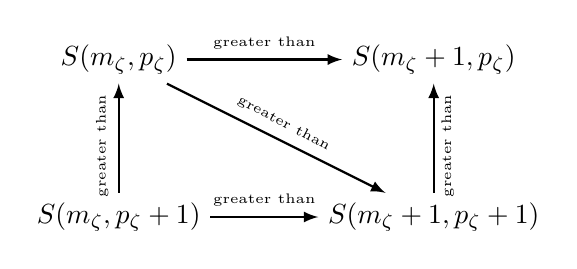
\begin{tikzpicture}
    \node[] (S00) at (0,0) {$S(m_\zeta,p_\zeta)$};
    \node[] (S10) at (4,0) {$S(m_\zeta+1,p_\zeta)$};
    \node[] (S01)  at (0,-2) {$S(m_\zeta,p_\zeta+1)$};
    \node[] (S11)  at (4,-2) {$S(m_\zeta+1,p_\zeta+1)$};
    
    \draw[->,thick,>=latex] (S00) -- node[anchor=south] {\tiny{greater than}} (S10);
    \draw[->,thick,>=latex] (S01) -- node[anchor=south] {\tiny{greater than}} (S11);
    \draw[->,thick,>=latex] (S11) -- node[anchor=west,xshift=5,yshift=-25,rotate=90] {\tiny{greater than}} (S10);

    \draw[->, thick,>=latex] (S00) -- node[anchor=south,rotate=-28] {\tiny{greater than}} (S11);
    \draw[->,thick,>=latex] (S01) -- node[anchor=west,xshift=-6,yshift=-25,rotate=90] {\tiny{greater than}} (S00);
\end{tikzpicture}
\caption{Behaviour of the landscape of Surprise $S$.}
\label{fig:surprisebehaviour}
\end{figure}

A fourth inequality $S(m_\zeta,p_\zeta+1)>S(m_\zeta+1,p_\zeta)$ is implicit by looking at the behaviour of $S(\zeta)$ for a given graph. The scheme in Figure \ref{fig:surprisebehaviour} allows to rank the values of Surprise in relation to changes in $m_\zeta$ and $p_\zeta$, in particular, it's easy to verify that $S$ satisfies the following strict order relation:
\begin{equation}\label{eq:surpriseorderrelation}
S(m_\zeta+1,p_\zeta)<S(m_\zeta+1,p_\zeta+1)<S(m_\zeta,p_\zeta)<S(m_\zeta,p_\zeta+1).
\end{equation}

In the convex interval $\mathcal{L}$ such that:
\begin{equation}
\mathcal{L} := \{ ( m_\zeta,p_\zeta) \; | m_\zeta > 0 \land p_\zeta \geq m_\zeta \land m \geq m_\zeta \land p-m > p_\zeta - m_\zeta \}
\end{equation}
Surprise is a monotonically increasing (decreasing $\hat{S}$) function of $p_\zeta$ and monotonically increasing function of $m_\zeta$ (increasing $\hat{S}$) as shown in Figure~\ref{fig:monotonical_surprise}.


\begin{figure}[htb]
\centering
\begin{tikzpicture}[scale=0.6, every node/.style={scale=0.6}]
\def \S {1};
\def \W {11};
\def \H {7};
\node[anchor=south west, inner sep=0mm] at (0,0) { \includegraphics[width=\W cm]{images/plot_surprise_pareto.pdf}};
\node[anchor=south] at (\W /2,\H +0.25) {$S(m_\zeta,p_\zeta$, $m=5$,$p=15$)};
%\draw[help lines,xstep=1.0,ystep=1.0] (0,0) grid (\W,\H);
\foreach \x in {1,...,\W } {\node [anchor=north] at (\x-0.5,0) {$\x$}; }
\node[anchor=north] at (\W/2,-0.5){$p_\zeta$};
\foreach \y in {1,...,\H} {\node [anchor=east] at (0 ,\y-0.5) {$\y$}; }
\node[anchor=east] at (-0.5,\H/2){$m_\zeta$};
%\node[rectangle,fill=black!10,draw=black,rounded corners=0.1cm] at (\W+1.5,\H-0.5) {$m_{\zeta},p_\zeta \not \subset \mathcal{L}$};
\end{tikzpicture}
\caption{Surprise increases as it gets hotter. The grey area is outside the domain of validity $\mathcal{L}$ while white are $S=0$.}
\label{fig:monotonical_surprise}
\end{figure}

Moreover, from Figure \ref{fig:surprisebehaviour} and Figure ~\ref{fig:monotonical_surprise} follows that an optimal solution with respect to $S$ is pareto-optimal with respect to maximizing $m_\zeta$ and minimizing $p_\zeta$.

With the tools of \ref{eq:surpriseorderrelation} in mind, one can infere how Surprise behaves under a perturbation of $m_\zeta$ and $p_\zeta$ by some amount $(\delta_{m_\zeta},\delta_{p_\zeta})$ and obtain a very useful tool that will help us in the rest of this work:
\begin{equation}\label{eq:resolution_limit_condition}
S(m_\zeta + \delta_{m_\zeta}, p_\zeta + \delta_{p_\zeta}) < S(m_\zeta,p_\zeta) \iff \delta_{m_\zeta} \geq \delta_{p_\zeta}
\end{equation}

The result in Eq.\ref{eq:resolution_limit_condition} is of great help in designing optimization algorithms as every move that increase the intracluster edges more than intracluster pairs is good, while moves that increase intracluster pairs more than intracluster edges must be ignored, therefore sparing time for the computation of Surprise. Additionally, Eq.\ref{eq:resolution_limit_condition} is a useful when analyzing the onset of the resolution limit for different models.
In the next sections we will also cast light on resolution limit for Surprise, to show with convincing theoretical arguments that $S$ is nearly resolution-limit-free in Traag's sense~\cite{traag2015}.

\section{Surprise is a statistic test}\label{sec:surprisefishertest}
It should be noted that \emph{Surprise} is the p-value of the one-tailed Fisher exact test. In particular one can draw the contingency table for the urn model as:

\begin{table}[htb]
\centering
\begin{tabular}{|c|c|c|c|}
\hline
 & Drawn & Not drawn & \textbf{Total}\\
\hline
Intracluster & $m_\zeta$ & $p_\zeta-m_\zeta$ & $p_\zeta$\\
\hline
Intercluster & $m-m_\zeta$ & $p-m-p_\zeta+m_\zeta$ & $p-p_\zeta$ \\
\hline
\textbf{Total} & $m$ & $p-m$ & $p$ \\
\hline
\end{tabular}
\end{table}
The odds-ratio $\textrm{OR} \in (0,\infty)$ of this $2\times 2$ contingency table is
\begin{equation}
\textrm{OR} = \frac{m_\zeta(p-m-p_\zeta+m_\zeta)}{(m-m_\zeta)(p_\zeta-m_\zeta)} 
\end{equation}
In particular minimizing Surprise corresponds to maximizing the odds-ratio $\textrm{OR}$. Very low values of $S$ tells us that we can reject the null hypothesis $H_0 := \textrm{OR} \neq 1$ with high probability.

It can be shown that when the entries of the contingency table are big enough, computing $S$ corresponds to computing the $\chi^2$ statistic and it is also possible to tackle the problem of computation of $S$ by means of odds-ratio.
If one computes the \emph{normalized log odds-ratio}:
\begin{equation}
\log(\textrm{OR}) = \log\left( \frac{m_\zeta(p-m-p_\zeta+m_\zeta)}{(m-m_\zeta)(p_\zeta-m_\zeta)} \right )
\end{equation}
and seeks the probability
\begin{equation}
\Pr\left(z < -\frac{|\log\textrm{OR})|}{SE} \right)
\end{equation}
where $z$ is a random variable with standard normal distribution $z \approx \mathcal{N}(0,1)$.
\section{Marginal Surprise}
The smart reader suddenly notes that the definition of subgraph probability is a natural way to measure the significance of the hypothesis that the particular observed value of subgraph \emph{internal} density is higher than the average graph density.
This concept relates to the degree to which subgraph nodes relates each other rather than to external nodes.

An opposite idea is to see to what level of significance the fraction of links that a subgraph is throwing \emph{outside} is smaller than what expected on the basis of the global graph properties.
In this respect, similarly to what is done for the subgraph probability in Eq.~\ref{eq:surprise} one may want to know what is the probability of observing the intercluster density of the subgraph $\mathcal{G}_c$, specified by

\begin{equation}
\rho_{\textrm{out}}(\mathcal{G}_c)=\frac{m_c^{\textrm{out}}}{n_c(n-n_c)}
\end{equation}

less than or equal to a fixed value in a subgraph drawn randomly from a graph with a given density $\rho=m/p$.
This concept is expressed in probabilistic form in the following equation:
\begin{align}\label{eq:centripetalsignificance}
\Pr[m^{\textrm{out}}_c \leq q ] &= \sum \limits_{i=0}^{q} \frac{\binom{m}{i}\binom{p-m}{n_c(n-n_c)-i)}}{\binom{p}{n_c(n-n_c)}} \nonumber \\ 
& = \sum \limits_{i=0}^{q} \frac{\binom{n_c(n-n_c)}{i}\binom{p-n_c(n-n_c)}{m-i}}{\binom{p}{m}}
\end{align}

But there is a refinement for equation \ref{eq:centripetalsignificance}:
\begin{align}
\Pr[m^{\textrm{out}}_c \leq q | m_c =r] &= \sum \limits_{i=0}^{q} \dfrac{\binom{m-r}{i} \binom{p-p_c - (m-r)}{n_c(n-n_c) - i}}{\binom{p-p_c}{n_c(n-n_c)}} \\
 &=  \sum \limits_{i=0}^{q} \dfrac{\binom{n_c(n-n_c)}{i}\binom{p-p_c-n_c(n-nc)}{m-r-i)}}{\binom{p-p_c}{m-r}}\\
  &=  1- \sum \limits_{i=q}^{m} \dfrac{\binom{n_c(n-n_c)}{i}\binom{p-p_c-(n_c(n-nc))}{m-r-i}}{\binom{p-p_c}{m-r}}
\end{align}

One wants to find a subgraph $\mathcal{G}=(\mathcal{V},\mathcal{E})$ with $|\mathcal{V}|=n_c$ nodes out of a graph with $n$ nodes, partitions the total number of edges in the graph $G$ as the sum of three contributes, $m_c=|\mathcal{E}|$ that is the number of edges of $\mathcal{G}$, the number of edges that $\mathcal{G}$ projects to the rest of the graph, that we call $m^{\textrm{out}}_c$ and the number of edges that have no endpoint in $\mathcal{G}$ that we call $m_{\tilde{c}}$:

\begin{equation}
m = m_c + m^{\textrm{out}}_c + m_{\tilde{c}}
\end{equation}

For fixed $m$, the larger $m_c$ is, the stricter is the upper bound on $m^{\textrm{out}}_c$. Hence a better test of how probable a particular value of $m^{\textrm{out}}_c$ is, would involve computing the probability under the assumption that $m_c$ is fixed as its observed value; that is, a better test would involve computing the conditional probability $\Pr[m^{\textrm{out}}_c \leq q | m_c =r]$.

To compute this probability, it is sufficient to reduce the graph by $p$ pairs of nodes of which $r$ are edges, and then to compute the probability of observing $q$ or fewer edges in a randomly drawn set containing $L(n,N)$ pairs of nodes. This probability is given by the expression:

\begin{align}\label{eq:hyperrefinement}
\Pr[m^{\textrm{out}}_c \leq q | m_c =r] &= \sum \limits_{i=0}^{q} \dfrac{\binom{m-r}{i} \binom{p-p_c - (m-r)}{n_c(n-n_c) - i}}{\binom{p-p_c}{n_c(n-n_c)}} \\
&=  \sum \limits_{i=0}^{q} \dfrac{\binom{n_c(n-n_c)}{i}\binom{(p-p_c)-(n_c(n-nc)))}{(m-r)-i)}}{\binom{(p-p_c)}{m-r}}
\end{align}


Figure \ref{fig:subgraphconditionalprobability} shows the settings of this problem. A random subgraph $\mathcal{G}$ is chosen, consisting in nodes $\{e,f,g,h\}$, the remaining nodes form the subgraph $G-\mathcal{G}$.
\begin{figure}[htb]
\centering
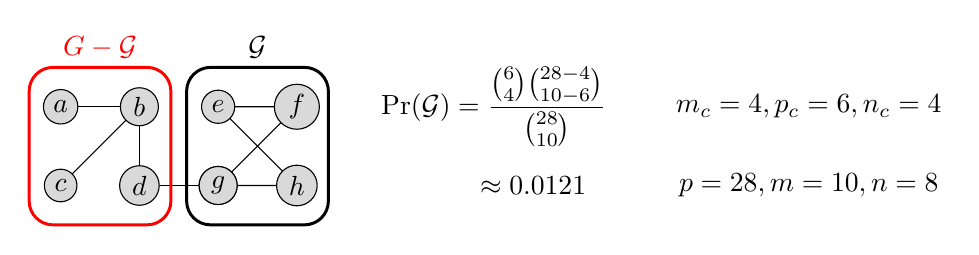
\begin{tikzpicture}
%\draw[help lines,step=1] (-4,-4) grid (8,4);
\draw [rectangle, black, draw, rounded corners=2ex,line width=0.25ex] (1.6,-0.5) rectangle (3.4,1.5);

\draw (1,0) -- (3,0);
\draw (2,1) -- (3,1) -- (2,0) -- (3,0) -- cycle;
\node [fill=gray!30, radius=1ex, draw, circle, inner sep=2pt] at (2,1) {$e$};
\node [fill=gray!30, radius=1ex, draw, circle, inner sep=2pt] at (3,1) {$f$};
\node [fill=gray!30, radius=1ex, draw, circle, inner sep=2pt] at (2,0) {$g$};
\node [fill=gray!30, radius=1ex, draw, circle, inner sep=2pt] at (2,0) {$g$};
\node [fill=gray!30, radius=1ex, draw, circle, inner sep=2pt] at (3,0) {$h$};
\draw (0,1) -- (1,1);
\draw (1,1) -- (1,0);
\draw (1,0) -- (1,1);
\draw (1,1) -- (0,0);
\node [fill=gray!30, radius=1ex, draw, circle, inner sep=2pt] at (0,1) {$a$};
\node [fill=gray!30, radius=1ex, draw, circle, inner sep=2pt] at (1,1) {$b$};
\node [fill=gray!30, radius=1ex, draw, circle, inner sep=2pt] at (0,0) {$c$};
\node [fill=gray!30, radius=1ex, draw, circle, inner sep=2pt] at (1,0) {$d$};
\node at (2.5,1.75) {$\mathcal{G}$};
\node at (0.5,1.75) {{\color{red}$G-\mathcal{G}$}};
\draw [rectangle, red, draw, rounded corners=2ex,line width=0.25ex] (-0.4,-0.5) rectangle (1.4,1.5);
\node [] at (5.5,1) {$\Pr(\mathcal{G}) = \dfrac{\binom{6}{4} \binom{28-4}{10-6}}{\binom{28}{10}}$};
\node [] at (6.0,0) {$\approx 0.0121$};

\node [] at (9.5,1) {$m_c=4,p_c=6,n_c=4$};
\node [] at (9.5,0) {$p=28,m=10,n=8$};
\end{tikzpicture}
\caption{Probability for the subgraph $\mathcal{G}=(\mathcal{V},\mathcal{E})$ where $\mathcal{V}=\{e,f,g,h\}$ and $\mathcal{E}=\{(e,f),(f,g),(g,h),(e,h)\}$ to be randomly drawn from the graph $G$.}
\label{fig:subgraphconditionalprobability}
\end{figure}


This last formula corresponds to an urn model where the number of balls in the urn is $p-p_c$, the number of white balls in the urn is $n_c(n-n_c)$, the number of drawn balls is $m-r$ and the number of white extracted balls in $q$.

The probability of a partition is then the marginal distribution of Eq. \ref{eq:hyperrefinement}, obtained by summing over all values of $r$ from $0$ to $m$.

\begin{equation}
\mathcal{S}_m =  \sum \limits_{r=0}^m \Pr[m^{\textrm{out}}_c \leq q | m_c =r]
\end{equation}

% \end{appendices}

%\printindex
\end{document}
